\clearpage
%%%%%%%%%%%%%%%%%%%%%%%%%%%%%%%%%%%%%

\section{Event selection}
\label{sec:selection}

The event selection is divided in two steps. At first, a set of cuts related to trigger and physics object (muons and photons) selection is applied. High level physics objects at CMS are reconstructed based of the Particle Flow (PF) algorithm \cite{PF_paper_2016}. This selection is called, within this analysis, Group I. 

For the events that pass the Group I selection, another set of cuts is applied, this time focusing on kinematical (phase space) event selection, in order to enhance the signal to background ratio. This later set is called, within this analysis, Group II. After full selection, three exclusive categories are defined, based on the photon's $\eta$ region and its energy spread shape within the ECAL cells (R9).

% It was a deliberated choice to apply on this analysis the same event selection of the $H/Z \rightarrow J/\psi + \gamma$  with 2016 data. Full documentation on this analysis can be found at \cite{CMS_jpsi_analysis}. Since the two analyses are similar, not only in final state, but also on the kind of intermediate meson ($\Upsilon$ or $J/\psi$) and energy scale, this choice was taken in order to keep the compatibility of the two studies. The only difference in the event selection is the dimuon mass window, which was changed to a suitable cut for a $\Upsilon$ selection.  

After the full selection, a background and signal modeling process is applied, based on the invariant mass distributions, which will be explained in the next section.


%%%%%%%%%%%%%%%%%%%%%%%%%%%%%%%%%%%%%%%%%%%%%%%%%%%%%%%%%%%%%%%%%%%%%%%%%%%%%%%%%%%%%%%%%%%%%%%%%%%%%%%%%%%%%%%%%%%%%%%%
%%%%%%%%%%%%%%%%%%%%%%%%%%%%%%%%%%%%%%%%%%%%%%%%%%%%%%%%%%%%%%%%%%%%%%%%%%%%%%%%%%%%%%%%%%%%%%%%%%%%%%%%%%%%%%%%%%%%%%%%
%%%%%%%%%%%%%%%%%%%%%%%%%%%%%%%%%%%%%%%%%%%%%%%%%%%%%%%%%%%%%%%%%%%%%%%%%%%%%%%%%%%%%%%%%%%%%%%%%%%%%%%%%%%%%%%%%%%%%%%%
%%%%%%%%%%%%%%%%%%%%%%%%%%%%%%%%%%%%%%%%%%%%%%%%%%%%%%%%%%%%%%%%%%%%%%%%%%%%%%%%%%%%%%%%%%%%%%%%%%%%%%%%%%%%%%%%%%%%%%%%
%%%%%%%%%%%%%%%%%%%%%%%%%%%%%%%%%%%%%%%%%%%%%%%%%%%%%%%%%%%%%%%%%%%%%%%%%%%%%%%%%%%%%%%%%%%%%%%%%%%%%%%%%%%%%%%%%%%%%%%%
%%%%%%%%%%%%%%%%%%%%%%%%%%%%%%%%%%%%%%%%%%%%%%%%%%%%%%%%%%%%%%%%%%%%%%%%%%%%%%%%%%%%%%%%%%%%%%%%%%%%%%%%%%%%%%%%%%%%%%%%
%%%%%%%%%%%%%%%%%%%%%%%%%%%%%%%%%%%%%%%%%%%%%%%%%%%%%%%%%%%%%%%%%%%%%%%%%%%%%%%%%%%%%%%%%%%%%%%%%%%%%%%%%%%%%%%%%%%%%%%%
%%%%%%%%%%%%%%%%%%%%%%%%%%%%%%%%%%%%%%%%%%%%%%%%%%%%%%%%%%%%%%%%%%%%%%%%%%%%%%%%%%%%%%%%%%%%%%%%%%%%%%%%%%%%%%%%%%%%%%%%
%%%%%%%%%%%%%%%%%%%%%%%%%%%%%%%%%%%%%%%%%%%%%%%%%%%%%%%%%%%%%%%%%%%%%%%%%%%%%%%%%%%%%%%%%%%%%%%%%%%%%%%%%%%%%%%%%%%%%%%%
%%%%%%%%%%%%%%%%%%%%%%%%%%%%%%%%%%%%%%%%%%%%%%%%%%%%%%%%%%%%%%%%%%%%%%%%%%%%%%%%%%%%%%%%%%%%%%%%%%%%%%%%%%%%%%%%%%%%%%%%
%%%%%%%%%%%%%%%%%%%%%%%%%%%%%%%%%%%%%%%%%%%%%%%%%%%%%%%%%%%%%%%%%%%%%%%%%%%%%%%%%%%%%%%%%%%%%%%%%%%%%%%%%%%%%%%%%%%%%%%%
%%%%%%%%%%%%%%%%%%%%%%%%%%%%%%%%%%%%%%%%%%%%%%%%%%%%%%%%%%%%%%%%%%%%%%%%%%%%%%%%%%%%%%%%%%%%%%%%%%%%%%%%%%%%%%%%%%%%%%%%
%%%%%%%%%%%%%%%%%%%%%%%%%%%%%%%%%%%%%%%%%%%%%%%%%%%%%%%%%%%%%%%%%%%%%%%%%%%%%%%%%%%%%%%%%%%%%%%%%%%%%%%%%%%%%%%%%%%%%%%%
%
% _______  ______    _______  __   __  _______    ___  
%|       ||    _ |  |       ||  | |  ||       |  |   | 
%|    ___||   | ||  |   _   ||  | |  ||    _  |  |   | 
%|   | __ |   |_||_ |  | |  ||  |_|  ||   |_| |  |   | 
%|   ||  ||    __  ||  |_|  ||       ||    ___|  |   | 
%|   |_| ||   |  | ||       ||       ||   |      |   | 
%|_______||___|  |_||_______||_______||___|      |___| 
%
%%%%%%%%%%%%%%%%%%%%%%%%%%%%%%%%%%%%%%%%%%%%%%%%%%%%%%%%%%%%%%%%%%%%%%%%%%%%%%%%%%%%%%%%%%%%%%%%%%%%%%%%%%%%%%%%%%%%%%%%
%%%%%%%%%%%%%%%%%%%%%%%%%%%%%%%%%%%%%%%%%%%%%%%%%%%%%%%%%%%%%%%%%%%%%%%%%%%%%%%%%%%%%%%%%%%%%%%%%%%%%%%%%%%%%%%%%%%%%%%%
%%%%%%%%%%%%%%%%%%%%%%%%%%%%%%%%%%%%%%%%%%%%%%%%%%%%%%%%%%%%%%%%%%%%%%%%%%%%%%%%%%%%%%%%%%%%%%%%%%%%%%%%%%%%%%%%%%%%%%%%
%%%%%%%%%%%%%%%%%%%%%%%%%%%%%%%%%%%%%%%%%%%%%%%%%%%%%%%%%%%%%%%%%%%%%%%%%%%%%%%%%%%%%%%%%%%%%%%%%%%%%%%%%%%%%%%%%%%%%%%%
%%%%%%%%%%%%%%%%%%%%%%%%%%%%%%%%%%%%%%%%%%%%%%%%%%%%%%%%%%%%%%%%%%%%%%%%%%%%%%%%%%%%%%%%%%%%%%%%%%%%%%%%%%%%%%%%%%%%%%%%
%%%%%%%%%%%%%%%%%%%%%%%%%%%%%%%%%%%%%%%%%%%%%%%%%%%%%%%%%%%%%%%%%%%%%%%%%%%%%%%%%%%%%%%%%%%%%%%%%%%%%%%%%%%%%%%%%%%%%%%%
%%%%%%%%%%%%%%%%%%%%%%%%%%%%%%%%%%%%%%%%%%%%%%%%%%%%%%%%%%%%%%%%%%%%%%%%%%%%%%%%%%%%%%%%%%%%%%%%%%%%%%%%%%%%%%%%%%%%%%%%
%%%%%%%%%%%%%%%%%%%%%%%%%%%%%%%%%%%%%%%%%%%%%%%%%%%%%%%%%%%%%%%%%%%%%%%%%%%%%%%%%%%%%%%%%%%%%%%%%%%%%%%%%%%%%%%%%%%%%%%%
%%%%%%%%%%%%%%%%%%%%%%%%%%%%%%%%%%%%%%%%%%%%%%%%%%%%%%%%%%%%%%%%%%%%%%%%%%%%%%%%%%%%%%%%%%%%%%%%%%%%%%%%%%%%%%%%%%%%%%%%
%%%%%%%%%%%%%%%%%%%%%%%%%%%%%%%%%%%%%%%%%%%%%%%%%%%%%%%%%%%%%%%%%%%%%%%%%%%%%%%%%%%%%%%%%%%%%%%%%%%%%%%%%%%%%%%%%%%%%%%%
%%%%%%%%%%%%%%%%%%%%%%%%%%%%%%%%%%%%%%%%%%%%%%%%%%%%%%%%%%%%%%%%%%%%%%%%%%%%%%%%%%%%%%%%%%%%%%%%%%%%%%%%%%%%%%%%%%%%%%%%
%%%%%%%%%%%%%%%%%%%%%%%%%%%%%%%%%%%%%%%%%%%%%%%%%%%%%%%%%%%%%%%%%%%%%%%%%%%%%%%%%%%%%%%%%%%%%%%%%%%%%%%%%%%%%%%%%%%%%%%%
%%%%%%%%%%%%%%%%%%%%%%%%%%%%%%%%%%%%%%%%%%%%%%%%%%%%%%%%%%%%%%%%%%%%%%%%%%%%%%%%%%%%%%%%%%%%%%%%%%%%%%%%%%%%%%%%%%%%%%%%
%%%%%%%%%%%%%%%%%%%%%%%%%%%%%%%%%%%%%%%%%%%%%%%%%%%%%%%%%%%%%%%%%%%%%%%%%%%%%%%%%%%%%%%%%%%%%%%%%%%%%%%%%%%%%%%%%%%%%%%%
%%%%%%%%%%%%%%%%%%%%%%%%%%%%%%%%%%%%%%%%%%%%%%%%%%%%%%%%%%%%%%%%%%%%%%%%%%%%%%%%%%%%%%%%%%%%%%%%%%%%%%%%%%%%%%%%%%%%%%%%

\section{Trigger and physics object selection (Group I)}

\subsection{Trigger}
\label{sec:trigger}
% The trigger used to select events, At hardware level (called L1), it is seeded by at least one muon with $p_{T} > 5$ GeV (transverse momentum with respect to the proton beam line)  and a isolated E/$\gamma$ with $p_{T} > 18$ GeV. At software level (HLT), it is activated by at least one muon with $p_{T} > 17$ GeV and a Photon of $p_{T} > 30$ GeV.

In this study, the same trigger requirements are applied to both data and simulated samples. For the first trigger level (L1), events are selected if they present at least one muon with transverse momentum greater than 5 GeV and an isolated~\footnote{The concept of isolation will be detailed later, but in summary, it means a object which has very small activity (above a certain threshold of energy/momentum) around it. In hadron-hadron collider, isolation is a characteristics of hard interactions.} photon or electron with transverse momentum greater than 18 GeV (at L1, there is no differentiation between photons and electrons). At the software level of the trigger system (HLT), the events are required to have at least one muon with transverse momentum greater than 17 GeV and a photon with transverse momentum greater than 30 GeV.

In order to compensate any difference in the trigger performance between simulated and data samples, for every selected MC a proper scale factor is applied, based onthe\PT of the reconstructed muon and photon. These scale factor computed by the ratio between efficiency of the trigger for the Data sample over the efficiency for a MC sample. These efficiencies are calculated with the tag-and-probe method, exploring the resonance of a final state composed by two muon and one photon in the vicinity of the $Z$ boson invariant mass. To this final state, a selection was applied to ensure that the photon comes from a Final State Radiation process, allowing us to use the tag-and-probe method.

Considering the similarity of this analysis with the $H/Z \rightarrow J/\psi + \gamma$ analysis~\cite{papper_jpsi}, not only in term of data samples, but also for triggering and physics object selection, the same scale factors were applied. More details are given in the same paper.

\subsection{Muon Identification}
\label{sec:muon_id}
% After trigger selection, the same muon selection of the $H \rightarrow ZZ^{*} \rightarrow 4l$ is applied \cite{CMS_higgs_zz_4l}. This is the same approach used by the $H/Z \rightarrow J/\psi + \gamma$ analysis. 

Ahead of any selection, a standard CMS "Ghost Cleaning" procedure is applied to all reconstructed muons in order to avoid that a single physical muon is reconstructed as two or more. For this procedure, reconstructed muons sharing 50\% or more segments in the system are arbitrated, in such way, that the ones with lowest quality characteristic is excluded.

After the cleaning, a muon is chosen when it passes a two step identification: the \textbf{Loose ID} and the \textbf{Tight ID}. Below the muon identification procedure is summarized .

% One should keep in mind that the naming conventions for these definitions are exclusive for the $H \rightarrow ZZ^{*} \rightarrow 4l$ and, therefore, to this analysis, not corresponding to the Muon-POG definitions. 

For the Loose ID, each muon is required to:
\begin{itemize}
  \item have transverse momentum greater than 5 GeV, in order to cope with Particle Flow requirements;
  \item be within the muon system acceptance: $|\eta| < 2.4$;
  \item to have a three dimensional impact parameter uncertainty, with respect to the primary vertex, smaller than 4;
  \item to have transverse distance smaller than 0.5 cm ($d_{xy} < 0.5$), with respect to the primary vertex (PV);
  \item to have longitudinal distance smaller than 1.0 cm ($d_{z} < 1$), with respect to the primary vertex (PV).

  % \item reconstructed as \textbf{Global Muon} or \textbf{Tracker Muon};
  % \item muon tracks only in the muon system are rejected;
  % \item muons with \texttt{muonBestTrackType==2} (standalone) are discarded.
\end{itemize}

Muons reconstructed only in the muon system, without a correspondence with the tracker, are rejected. The last three requirements of the Loose ID are imposed in order to suppress muons from in-flight decays.

The primary vertex itself, is determined as the reconstructed vertex with the biggest sum of $p_T^2$ in the event. This sum is performed, considering all the charged PF candidates clustered by the jet finding algorithms~\cite{Cacciari:2008gp,Cacciari:2011ma} and the MET, which is defined as the $p_T$ vector sum of all the charged and neutral PF candidates associated to that vertex. 

For the Tight ID, muons with transverse momentum $p_{T} < 200$ GeV, are required to have been reconstructed with the Particle Flow (PF) algorithm. If they have $p_{T} > 200$ GeV, they should reconstructed with the Particle Flow (PF) algorithm or satisfy the strict tracker requirements (defined in table~\ref{tab:Tracker_High_pT}).

\begin{table}[h]
  \caption{Conditions for a muon to pass the strict tracker requirements.}
    \begin{center}
    \begin{tabular}{l|l}
     % \hline
     \textbf{Requirement}         & \textbf{Technical definition}                 \\
      \hline
      Muon station matching          & Muon is matched to segments           \\
                                     & in at least two stations in the muon system        \\
      \hline                                                          
      Good $\pt$ measurement         & $\frac{\sigma_{\pt}}{\pt} < 0.3$      \\
      \hline
      Vertex compatibility ($x-y$)   & $d_{xy} < 2$~mm                       \\
      \hline
      Vertex compatibility ($z$)     & $d_{z} < 5$~mm                        \\
      \hline
      Pixel hits                     & At least one pixel hit                \\
      \hline
      Tracker hits                   & Hits in at least six tracker layers   \\
      \hline
    \end{tabular}
    
    \label{tab:Tracker_High_pT}
    \end{center}
\end{table}


To mitigate spurious signal in the detector that would mimic a muon, the leading muon (the one with highest $p_T$) is required to be isolated within a cone of radius $\Delta R = \sqrt{\smash[b]{\Delta \eta}^2 + {\Delta \phi}^2}< 0.3$ in the $\eta - \phi$ plane. The isolation is evaluated in terms of ${\cal I}^{\mu} < 0.35$, defined as:


\begin{equation}
\label{eqn:pfiso}
{\cal I}^{\mu} \equiv \Big( \sum \PT^\text{charged} +
                                 \max\left[ 0, \sum \PT^\text{neutral}
                                 +
                                  \sum \PT^{\cPgg}
                                 - \PT^\mathrm{PU}(\mu) \right] \Big)
                                 / \PT^{\mu}.
\end{equation}


The $\sum \PT^\text{charged}$ is the scalar sum of the transverse momenta of charged hadrons originating from the chosen primary vertex of the event. The $\sum \PT^\text{neutral}$ and $\sum \PT^{\cPgg}$ are the scalar sums of the transverse momenta for neutral hadrons and photons, respectively.  Since the isolation variable is particularly sensitive to energy deposits from pileup interactions, a $\PT^\text{PU}(\mu)$ contribution is subtracted, where $\PT^\mathrm{PU}(\PGm) \equiv 0.5 \times \sum_i \PT^{\mathrm{PU}, i}$, where $i$ runs over the momenta of the charged hadron PF candidates not originating from the primary vertex, and the factor of 0.5 corrects for the different fraction of charged and neutral particles in the cone. 


% The last requirement over the selected muons is that the leading muon should be relatively isolated, over the Particle Flow ($\text{RelPFiso}(\Delta R = 0.3) < 0.35$).


% \begin{equation}
% \text{RelPFiso} = \frac{\sum^\text{charged had.} \pt + \max(\sum^\text{neutral had.} \ET 
% + \sum^\text{photon} \ET - \Delta \beta, 0)}{\pt^\text{lepton}}
% \label{eqn:mupfiso}
% \end{equation}

% The $\Delta\beta$, defined as $\Delta\beta = \frac{1}{2} \sum^\text{charged had.}_\text{PU} \pt$ gives an estimate of the pileup contribution.  



One should keep in mind that this muon identification process is the same as the one used by the $H \rightarrow ZZ^{*} \rightarrow 4l$~\cite{higgs_zz_4l_papper}. This was done in order to keep in phase with other Higgs analysis inside the collaboration. After the muon identification, an appropriate scale factor is applied to the MC events based on the leading muon \PT and $\eta$, in order to correct any possible discrepancy between data and simulated samples. The scale factors were taken from the $H \rightarrow ZZ^{*} \rightarrow 4l$ analysis.

In order to cope with trigger requirements, the leading muon should have $\PT > 20$ GeV and the trailing muon $\PT > 4$ GeV.


\subsection{Photon Identification}
\label{sec:photon_id}

For the photon identification and selection, the standard CMS recommendation are followed. The Multivariate (MVA) Photon identification is used with a working point of 90\%, together with a electron veto procedure, to avoid misidentification of electrons as photons. Kinematically, the photons are requested to have transverse energy, with respect to the beam line, $E_{T} > 33$ GeV and reconstructed within the CMS acceptance for photons $|\eta_{SC}| < 2.5$\footnote{SC stands for Super Cluster of the reconstructed photon. It is the set of cell in the Electromagnetic Calorimeter used for the photon observation.}, excluding the Electromagnetic Calorimeter (ECAL) Barrel-Endcap intersections.

The threshold of 33 GeV for the photon transverse energy is driven by the trigger requirements. The selected photon, per event, is the one with highest $E_{T}$.


\subsection{Kinematical distributions}
\label{sec:kin_plots_group_1}

The selection described so far, is called Group I. The plots shown below are related to selected events after this set. 

Figures \ref{fig:pTMuons_ZtoUpsilon_Cat0} to \ref{fig:phiPhoton_ZtoUpsilon_Cat0} present the \PT, $\eta$ and $\phi$ distributions for the leading muon, trailing muon and the photon, for the \Z decaying into $\Upsilon(1S,2S,3S)$ + $\gamma$. 

Figures \ref{fig:pTUpsilon_and_Z_ZtoUpsilon_Cat0} to \ref{fig:phiUpsilon_and_Z_ZtoUpsilon_Cat0} present the \PT, $\eta$ and $\phi$ distributions for reconstructed $\Upsilon(nS)$ ($\mu\mu$ system) and the reconstructed boson ($\mu\mu\gamma$ system).

Figures \ref{fig:deltaR_ZtoUpsilon_Cat0} to \ref{fig:dimuon_mass_ZtoUpsilon_Cat0} present the $\Delta R = \sqrt{\Delta\eta^2 + \Delta\phi^2}$ between the photon and the muons, the $\Delta R$ distributions between reconstructed dimuon ($\mu\mu$) system and the photon, the absolute value of the $\Delta \phi$ between the leading muon and the photon, the ratio for the transverse momentum of the reconstructed Upsilon and the reconstructed Z mass ($p_{T}^{\mu\mu}/M_{\mu\mu\gamma}$), the ratio for the transverse energy of the reconstructed Photon and the reconstructed Z mass ($E_{T}^{\gamma}/M_{\mu\mu\gamma}$) and dimuon mass distribution of the reconstructed $\Upsilon(nS)$.

Figures \ref{fig:pTMuons_HtoUpsilon_Cat0} to \ref{fig:dimuon_mass_HtoUpsilon_Cat0} present the same variables, but for the Higgs decaying into $\Upsilon(1S,2S,3S)$ + $\gamma$ channel.

In all figures, the black dots are data collect by CMS while the blue distribution is related only to the signal Monte-Carlo generated samples. The observed difference between signal MC and Data is accounted to the lack of full background contribution for these histograms. Only Signal MC is being considered. The key point is to compare the shape of the distributions and how much they match before and after the selection.

For any presented plot, \textbf{Data} stands for data collected from real $pp$ collisions by CMS and \textbf{Signal}, stands for the distribution of events from a MC generated sample of signal events, as described in Section~\ref{sec:datasets}.

%CONTROL PLOTS
%%$\pT$ muon distributions for ZtoUpsilon_Cat0
\begin{figure}[!htbp]
\begin{center}
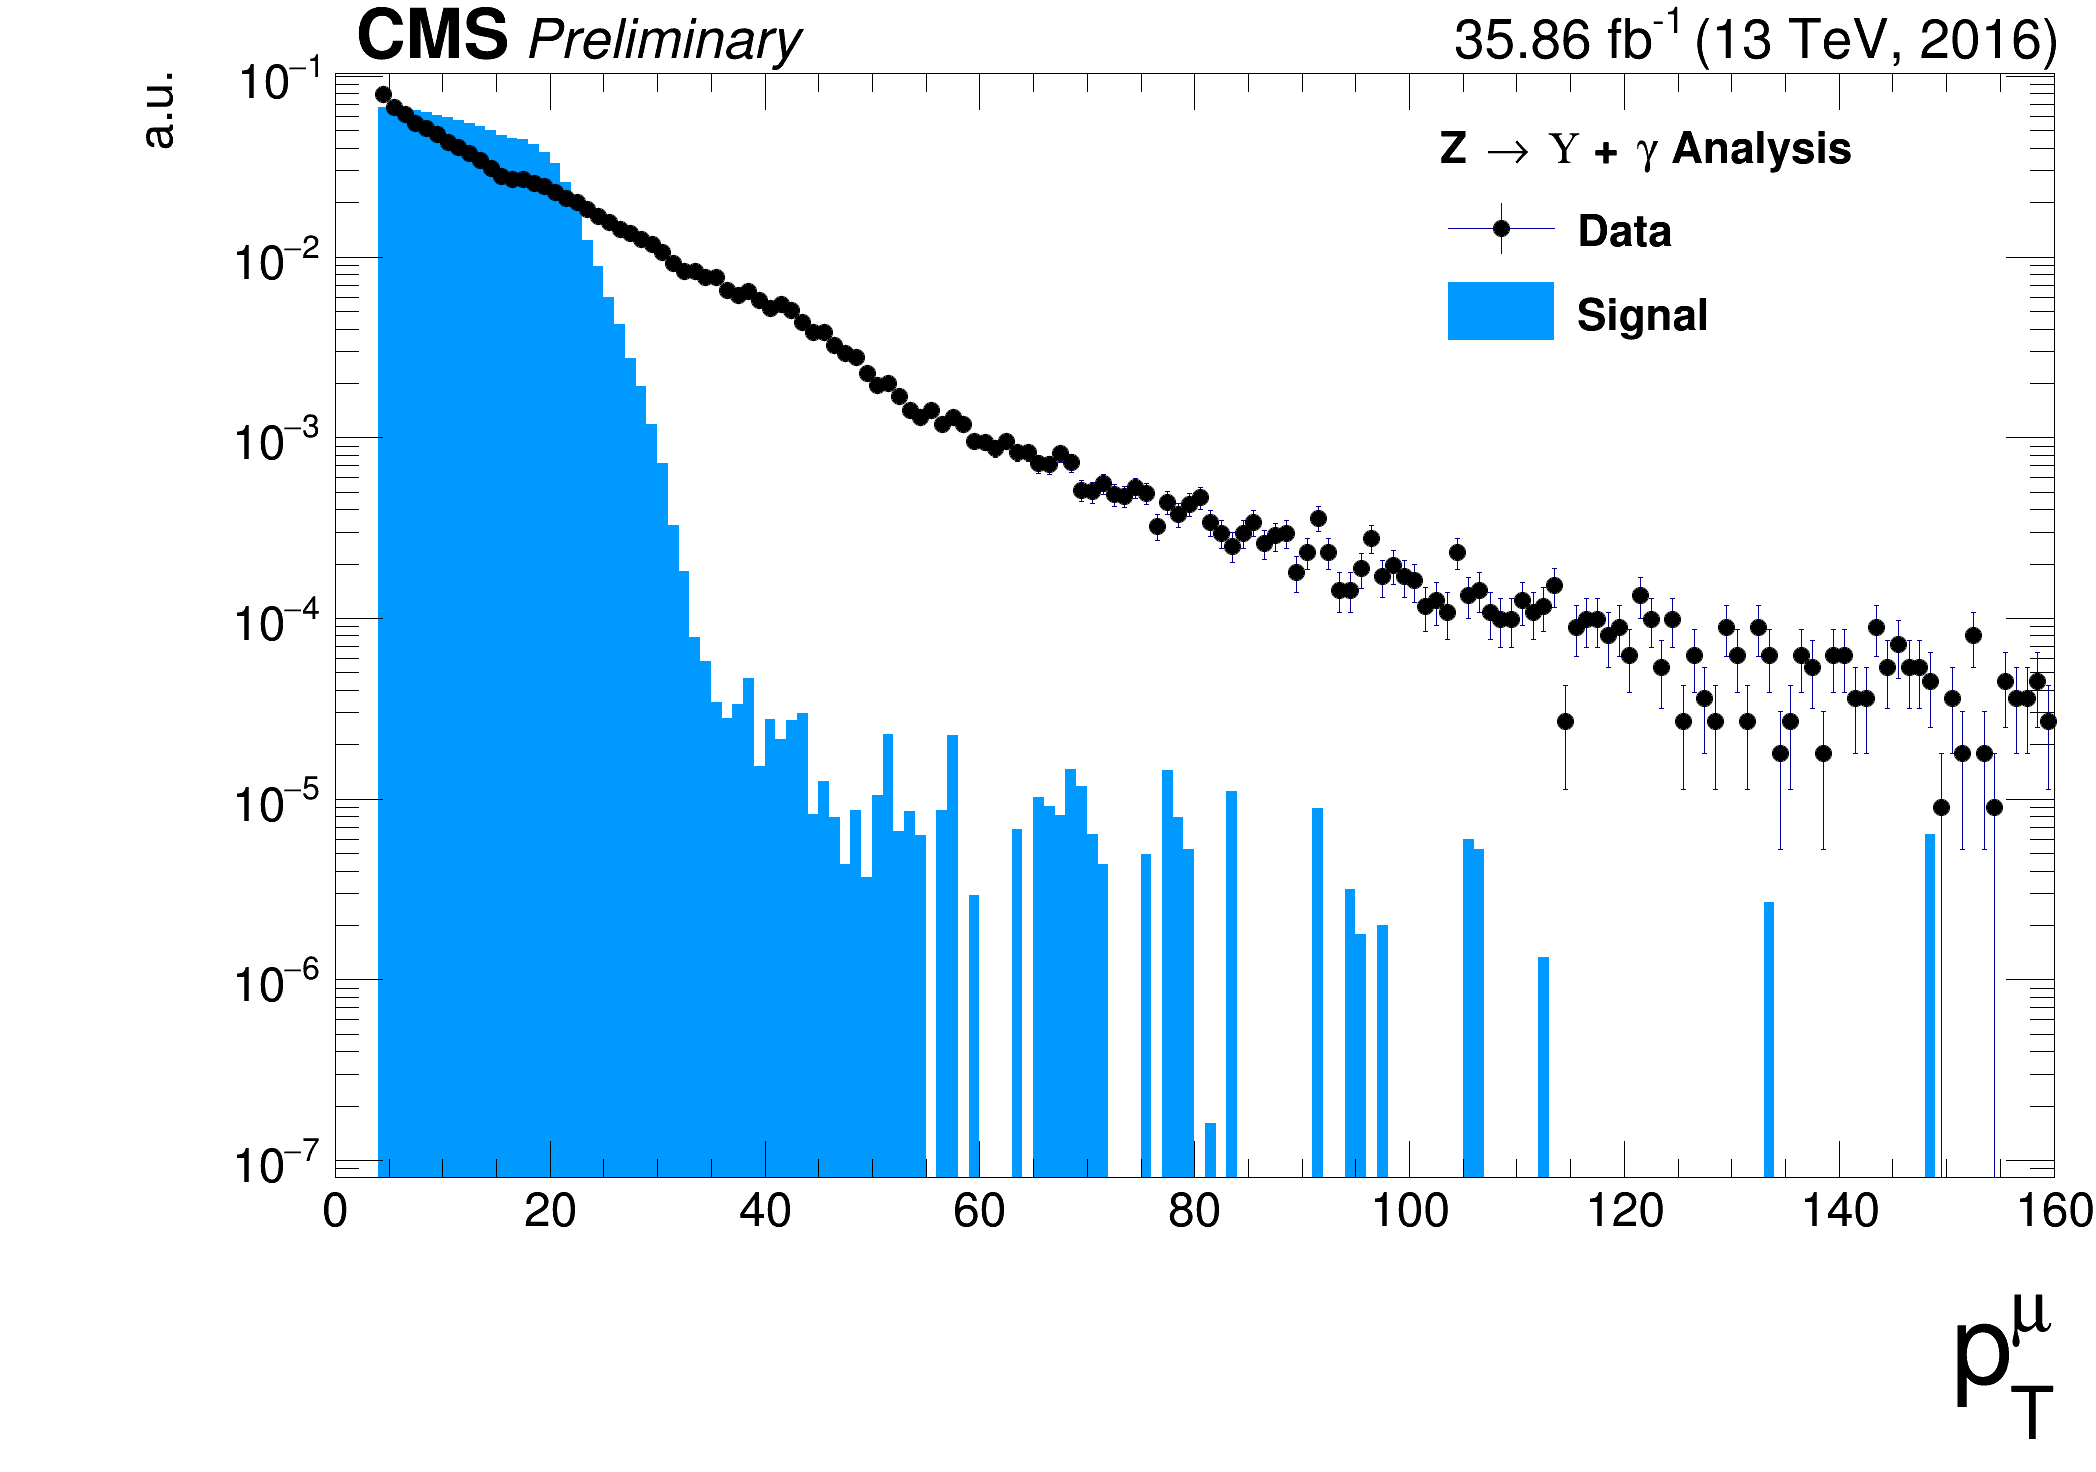
\includegraphics[width=0.45\textwidth]{figures_and_tables/outputPlots/ZtoUpsilon_Cat0_ZZZZZ/au/data_x_mc/noKinCuts/h_noKin_TrailingMu_pt}\hspace*{1.cm}
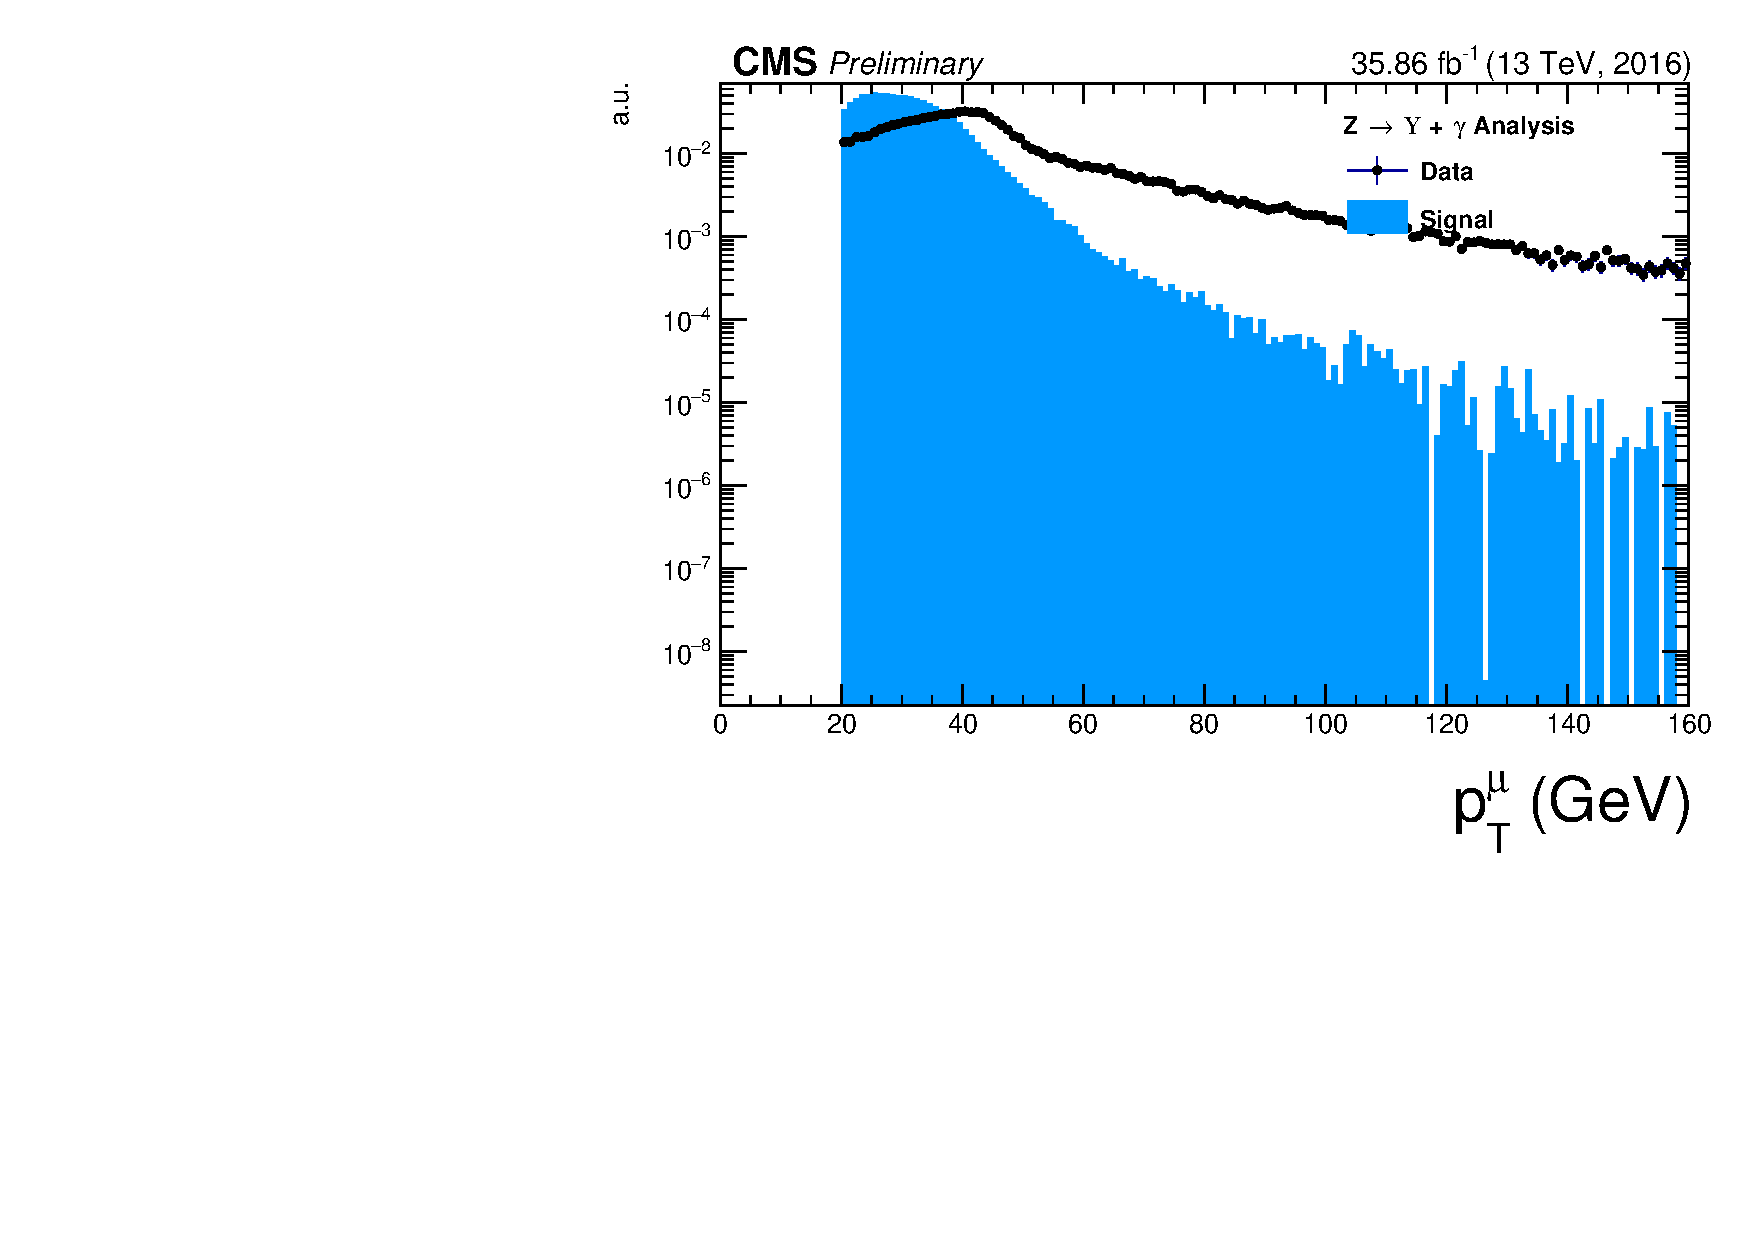
\includegraphics[width=0.45\textwidth]{figures_and_tables/outputPlots/ZtoUpsilon_Cat0_ZZZZZ/au/data_x_mc/noKinCuts/h_noKin_LeadingMu_pt}
\end{center}\vspace*{-.5cm}
\caption{The \PT muon distributions from data and signal events for \Z decaying into $\Upsilon(1S,2S,3S)$ + $\gamma$ after Group I of selection cuts, where on left are presenting the trailing muons and on right are the leading muons. The plots are normalized to the unit of area. The black dots are data collect by CMS while the blue distribution is related only to the signal Monte-Carlo generated samples.}
\label{fig:pTMuons_ZtoUpsilon_Cat0}
\end{figure}


%%%%%%%$\eta$ muon distributions for ZtoUpsilon_Cat0
\begin{figure}[!htbp]
\begin{center}
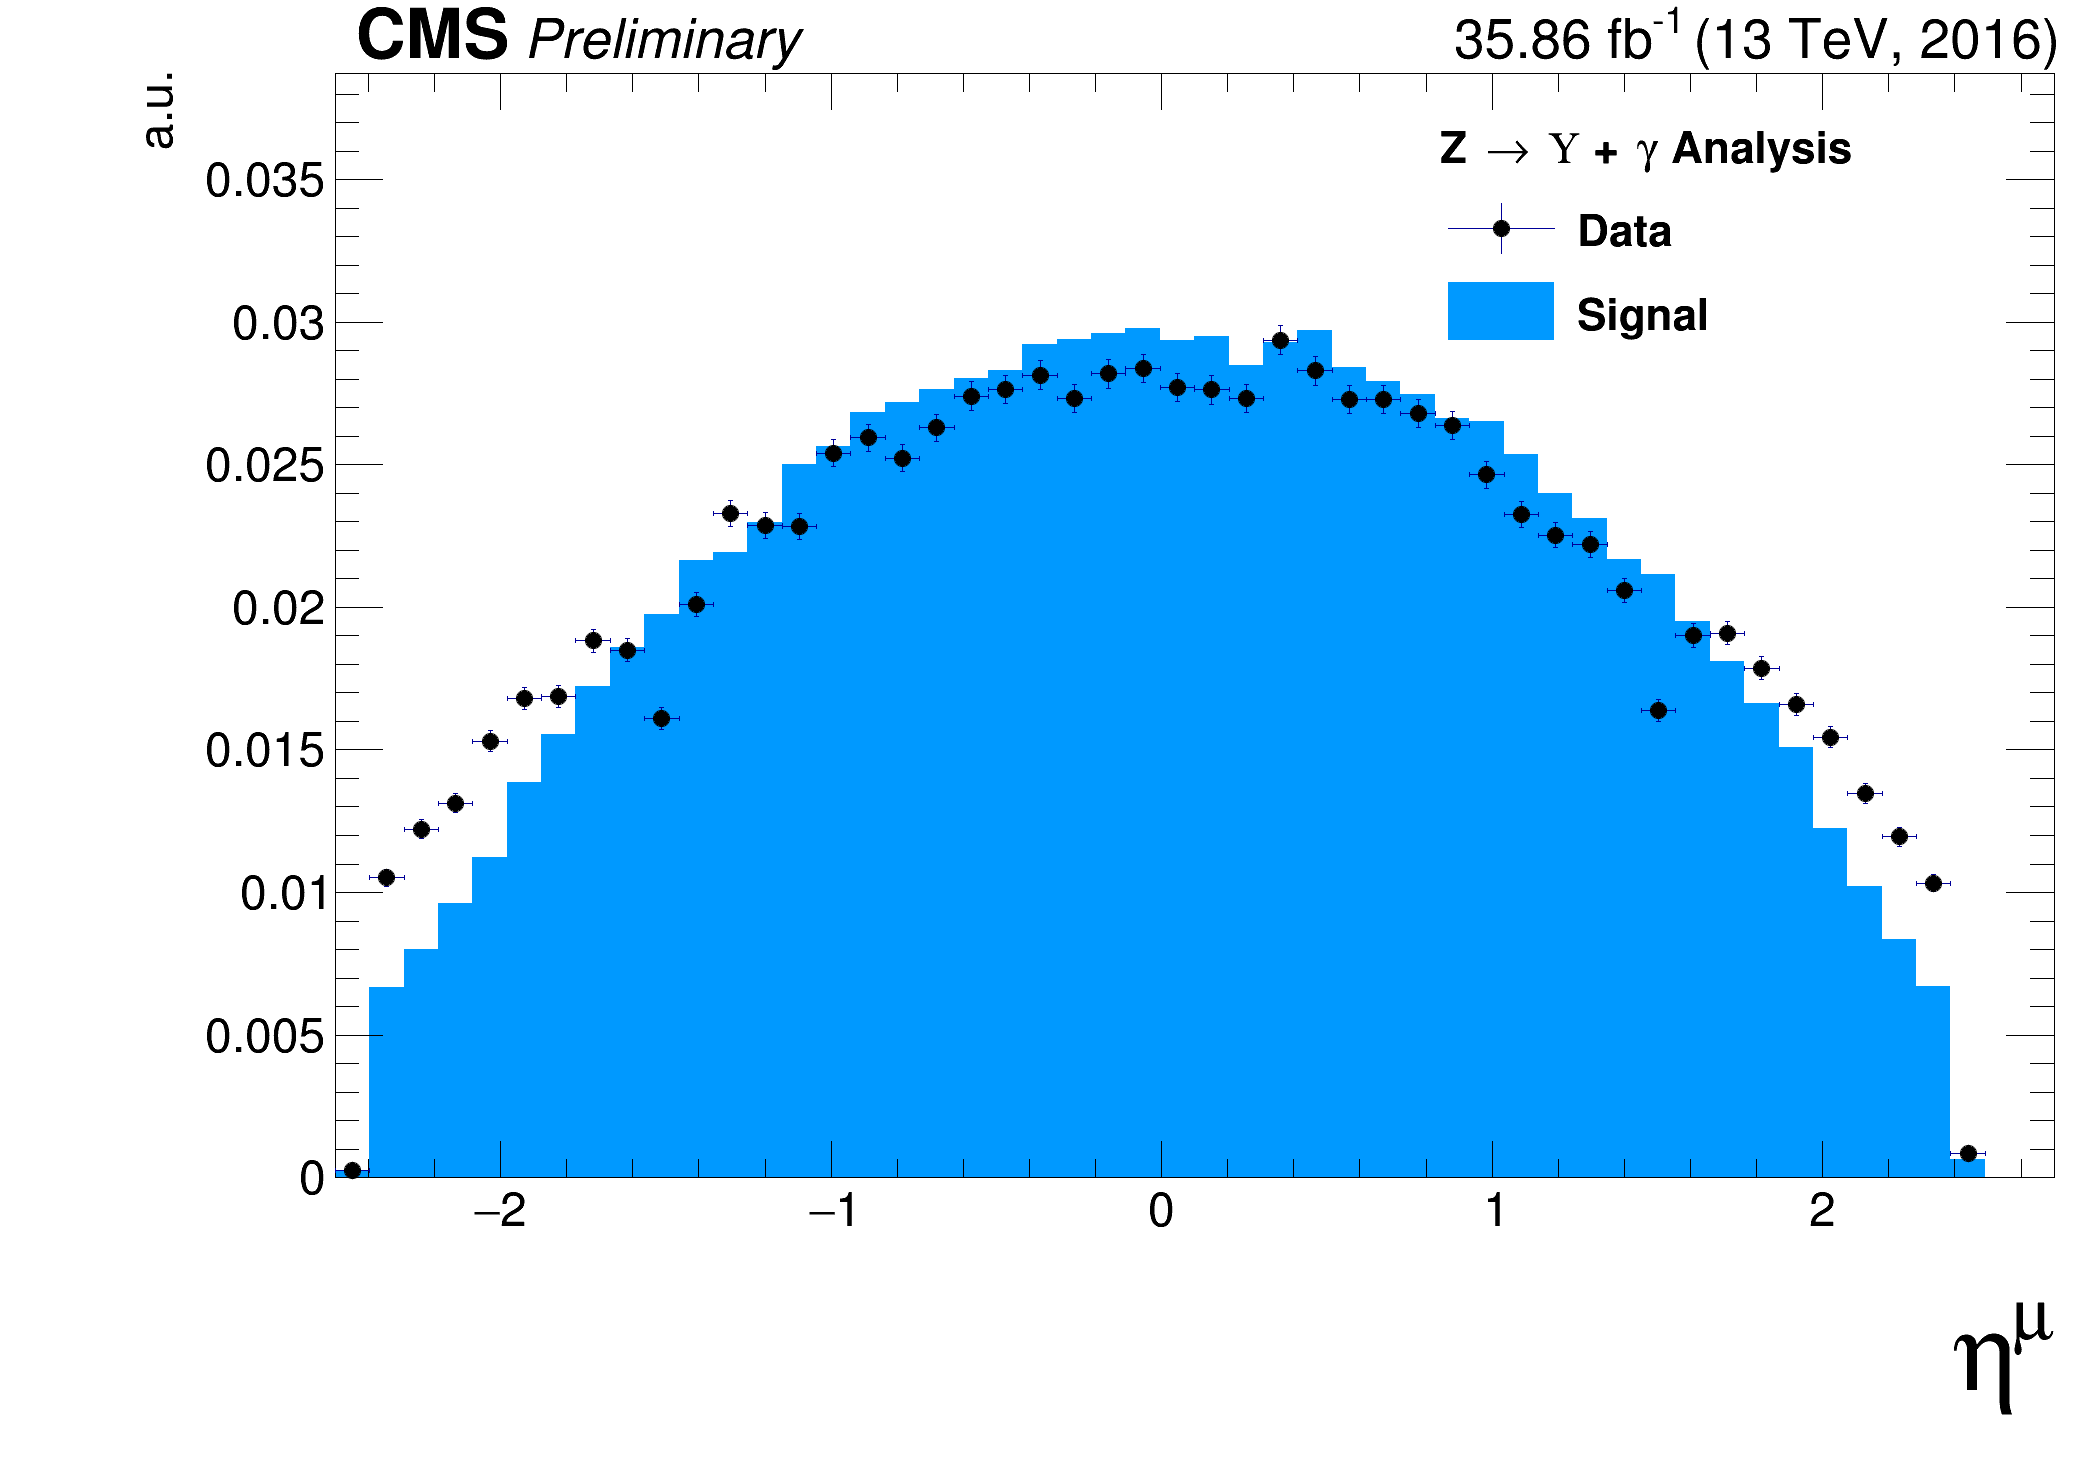
\includegraphics[width=0.45\textwidth]{figures_and_tables/outputPlots/ZtoUpsilon_Cat0_ZZZZZ/au/data_x_mc/noKinCuts/h_noKin_TrailingMu_eta}\hspace*{1.cm}
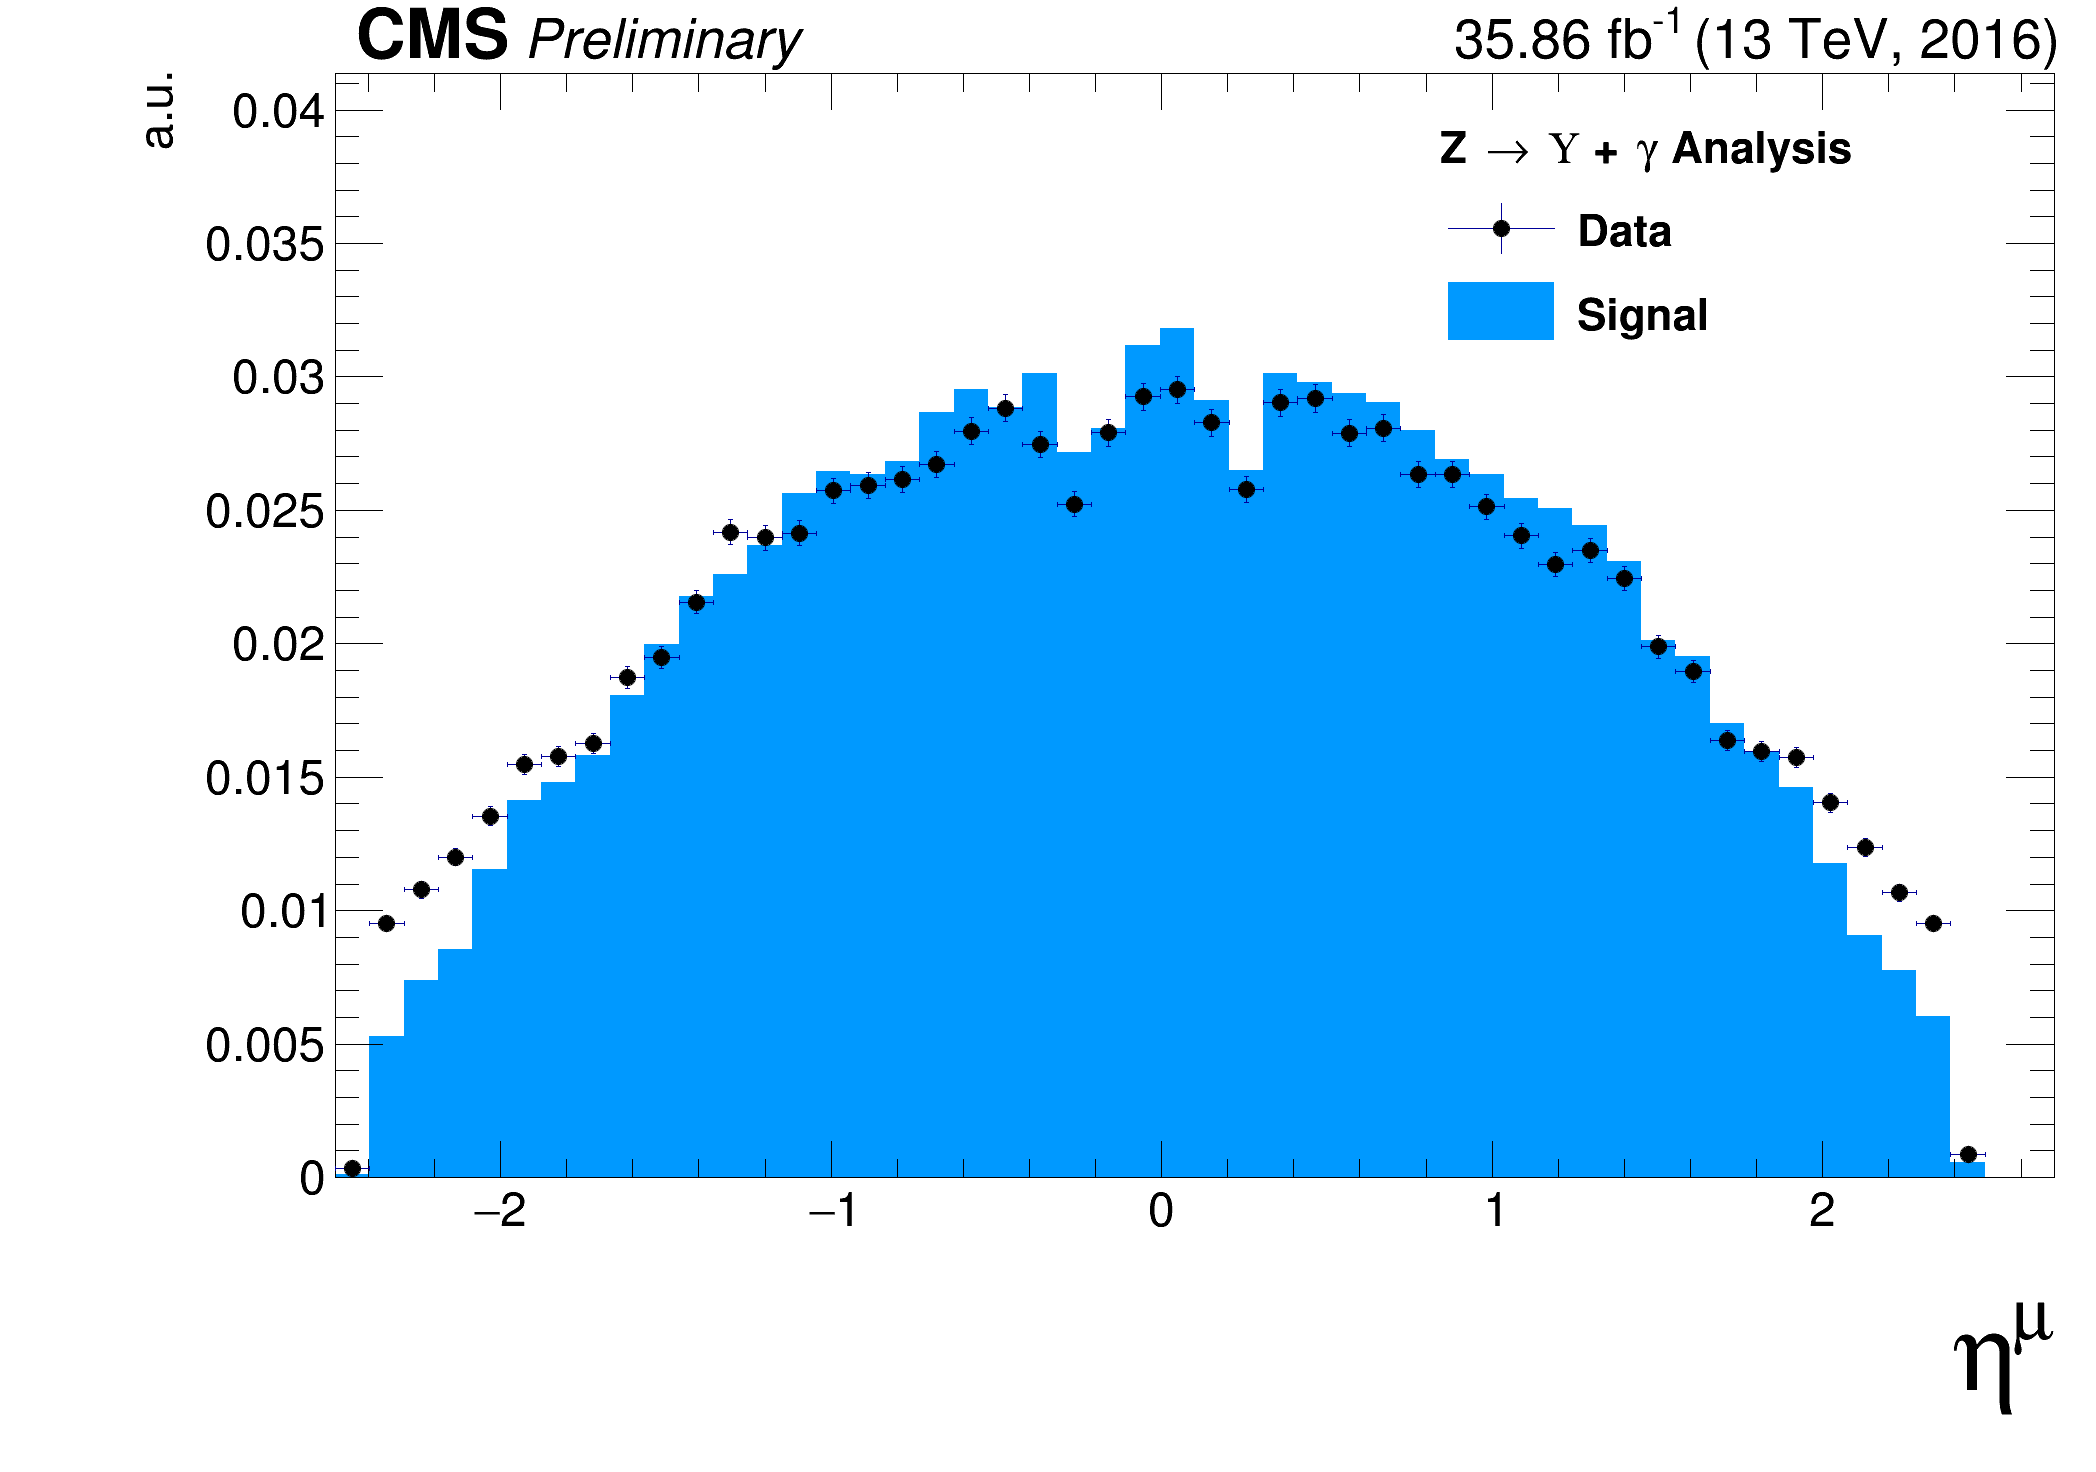
\includegraphics[width=0.45\textwidth]{figures_and_tables/outputPlots/ZtoUpsilon_Cat0_ZZZZZ/au/data_x_mc/noKinCuts/h_noKin_LeadingMu_eta}
\end{center}\vspace*{-.5cm}
\caption{The $\eta$ muon distributions from data and signal events of \Z decaying into $\Upsilon(1S,2S,3S)$ + $\gamma$ after Group I of selection cuts, where on left are presenting the trailing muons and on right are the leading muons. The plots are normalized to the unit of area. The black dots are data collect by CMS while the blue distribution is related only to the signal Monte-Carlo generated samples.}
\label{fig:etaMuons_ZtoUpsilon_Cat0}
\end{figure}

%%%%%%%%% $\phi$ muon distributions for ZtoUpsilon_Cat0
\begin{figure}[!htbp]
\begin{center}
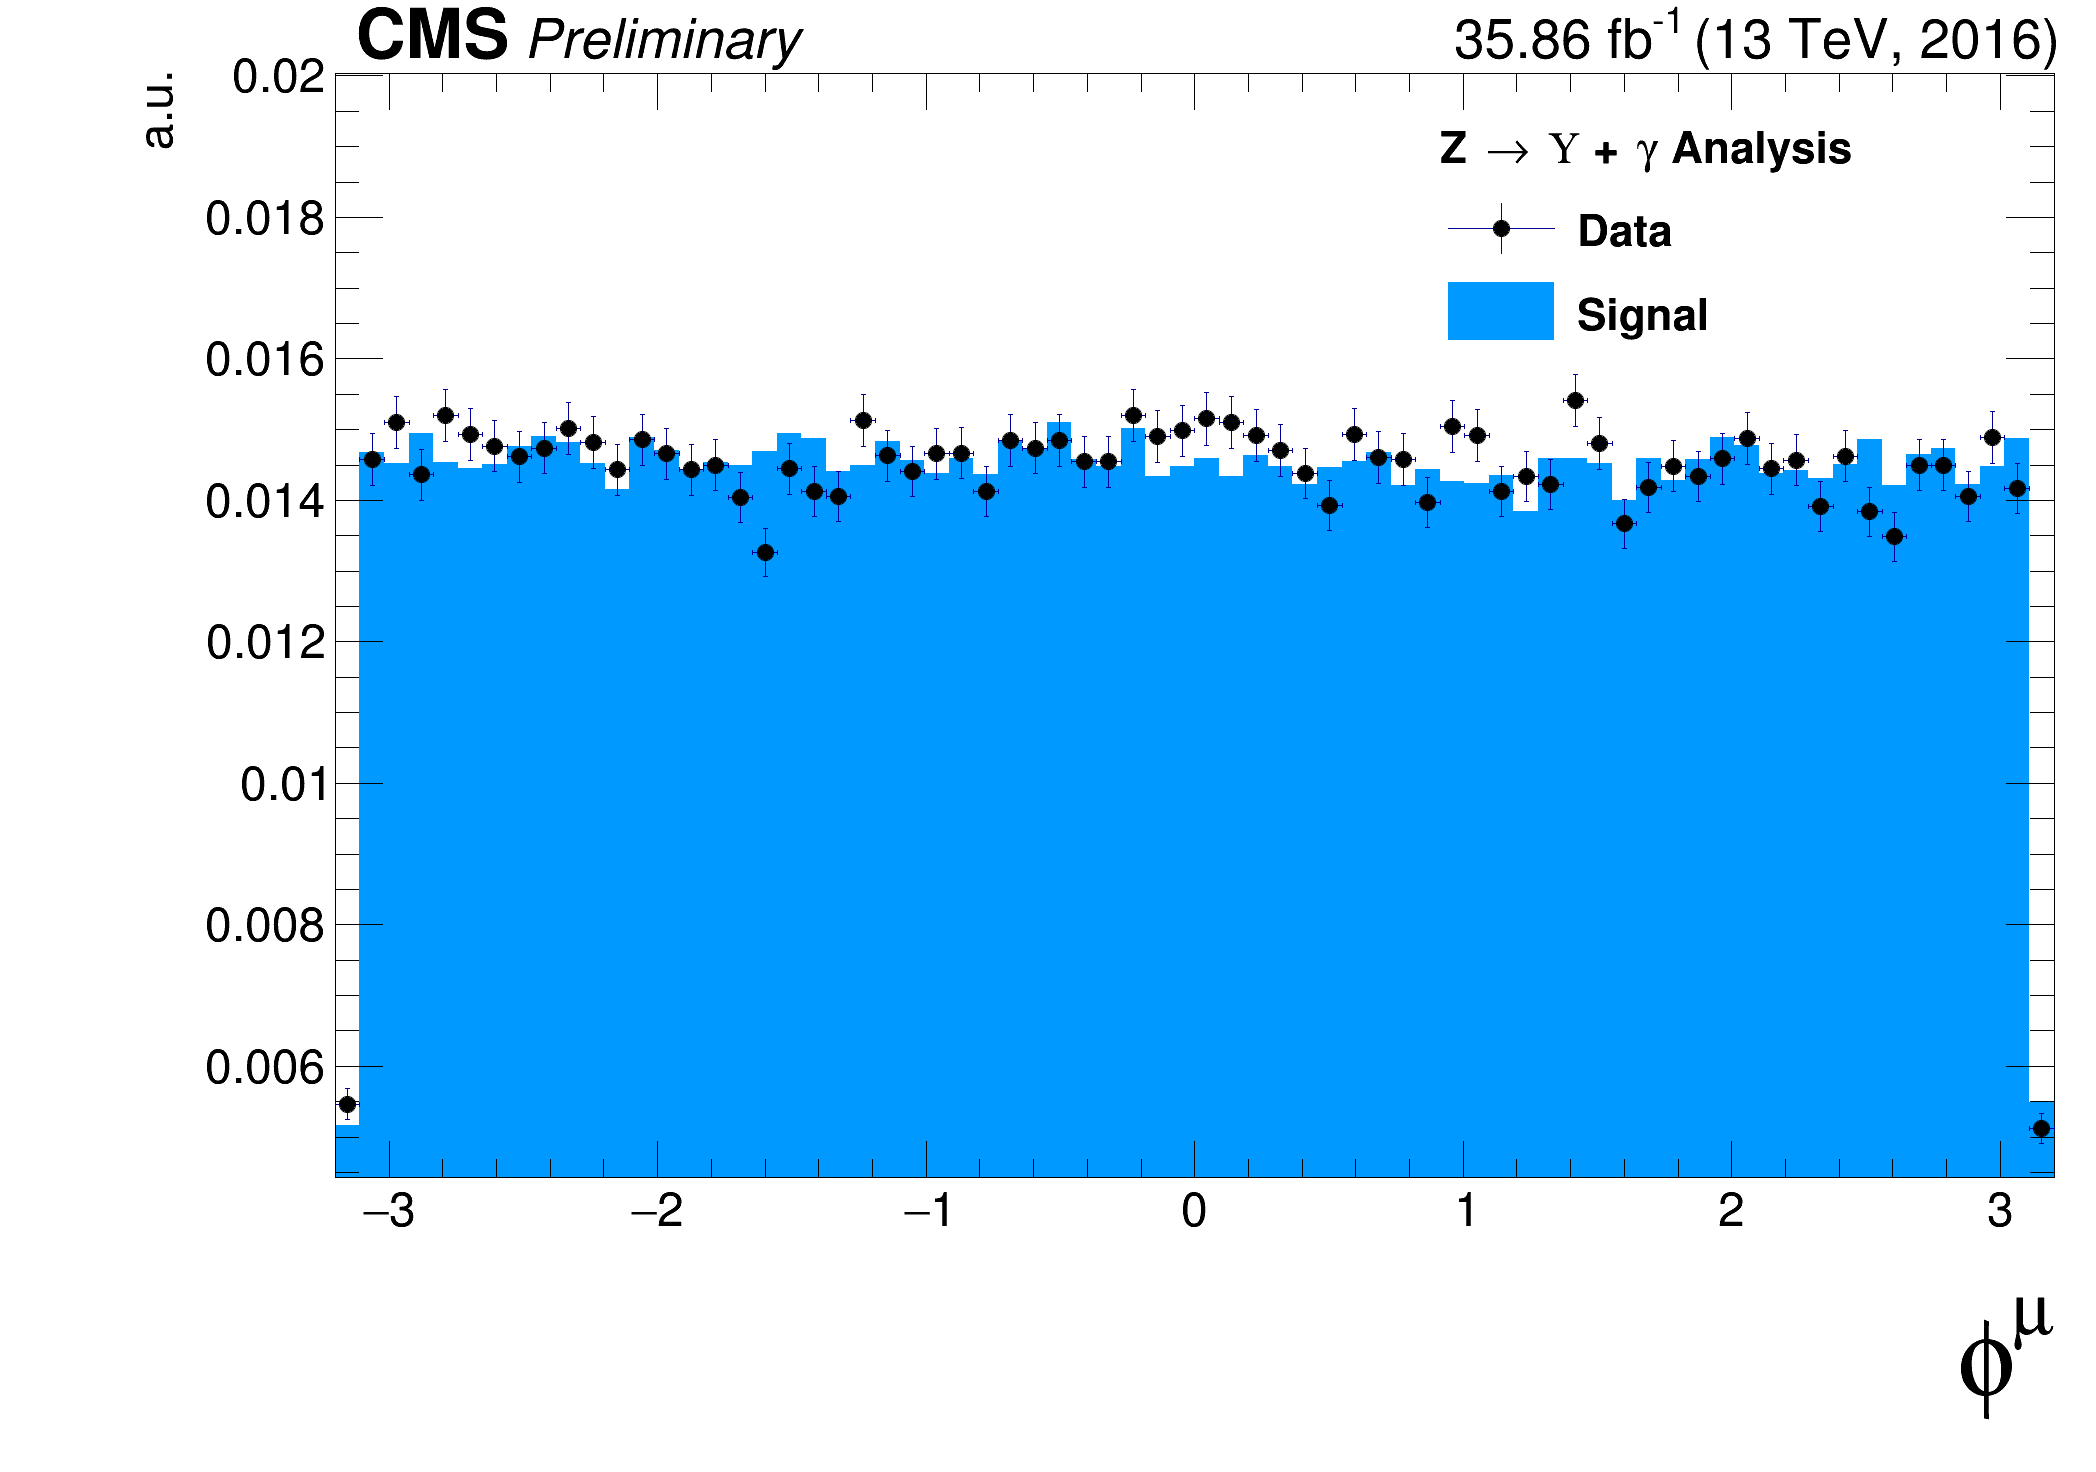
\includegraphics[width=0.45\textwidth]{figures_and_tables/outputPlots/ZtoUpsilon_Cat0_ZZZZZ/au/data_x_mc/noKinCuts/h_noKin_TrailingMu_phi}\hspace*{1.cm}
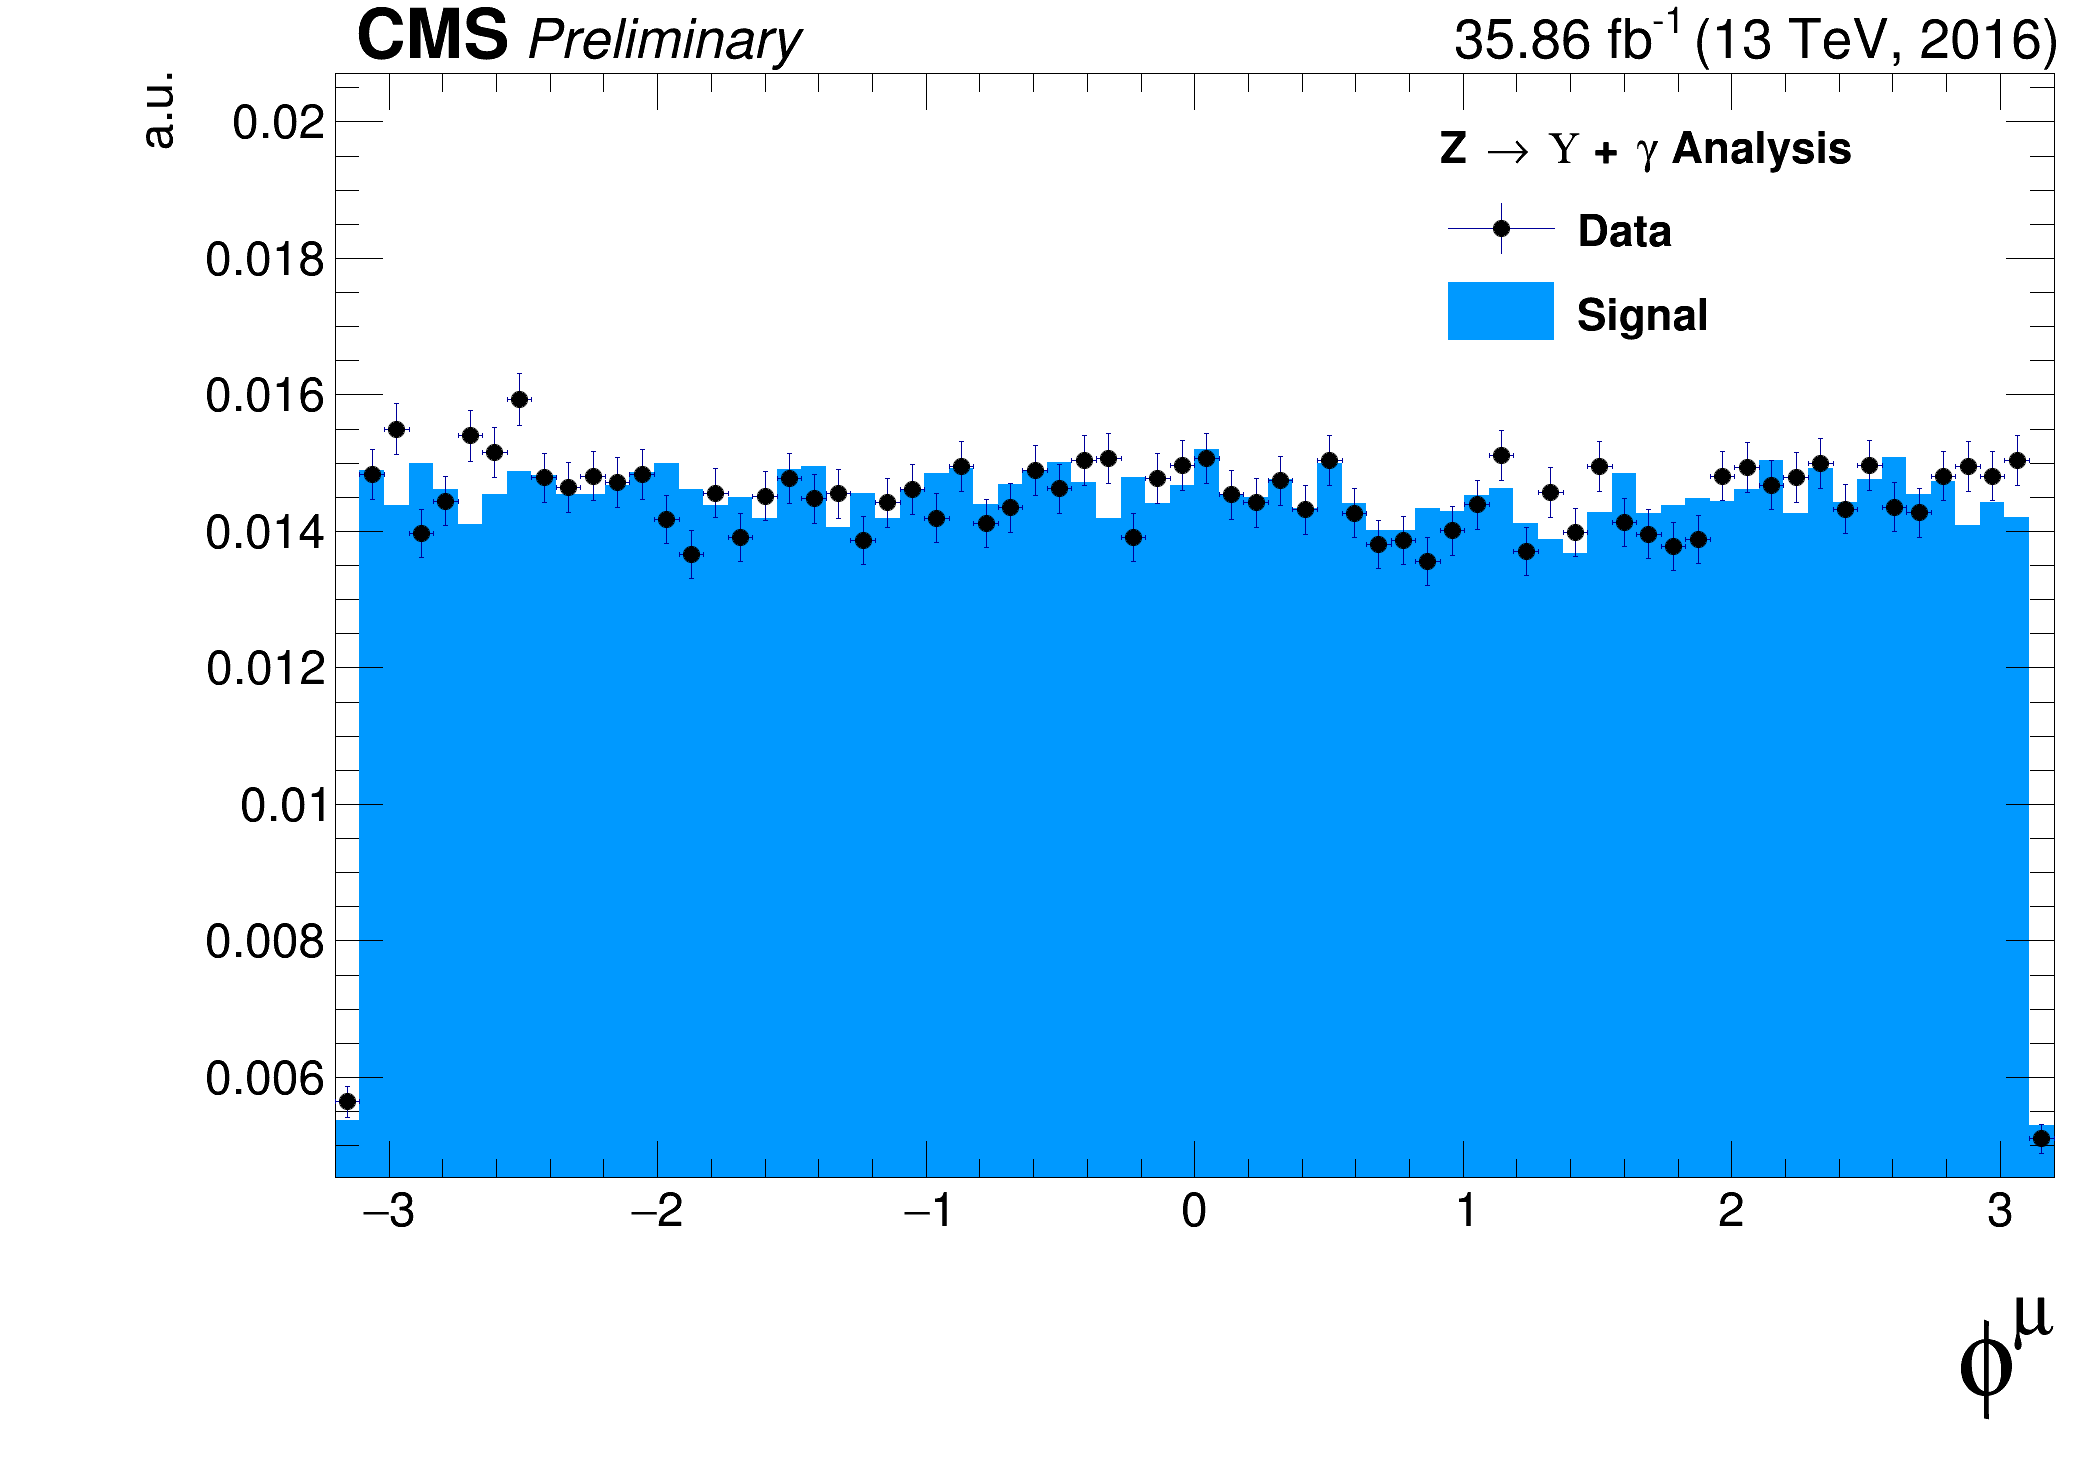
\includegraphics[width=0.45\textwidth]{figures_and_tables/outputPlots/ZtoUpsilon_Cat0_ZZZZZ/au/data_x_mc/noKinCuts/h_noKin_LeadingMu_phi}
\end{center}\vspace*{-.5cm}
\caption{The $\phi$ muon distributions from data and signal events of \Z decaying into $\Upsilon(1S,2S,3S)$ + $\gamma$ after Group I of selection cuts, where on left are presenting the trailing muons and on right are the leading muons. The plots are normalized to the unit of area. The black dots are data collect by CMS while the blue distribution is related only to the signal Monte-Carlo generated samples.}
\label{fig:phiMuons_ZtoUpsilon_Cat0}
\end{figure}

%%%%%%%%%%%%%

%photon
%%$\pT$ Photon distributions for ZtoUpsilon_Cat0
\begin{figure}[!htbp]
\begin{center}
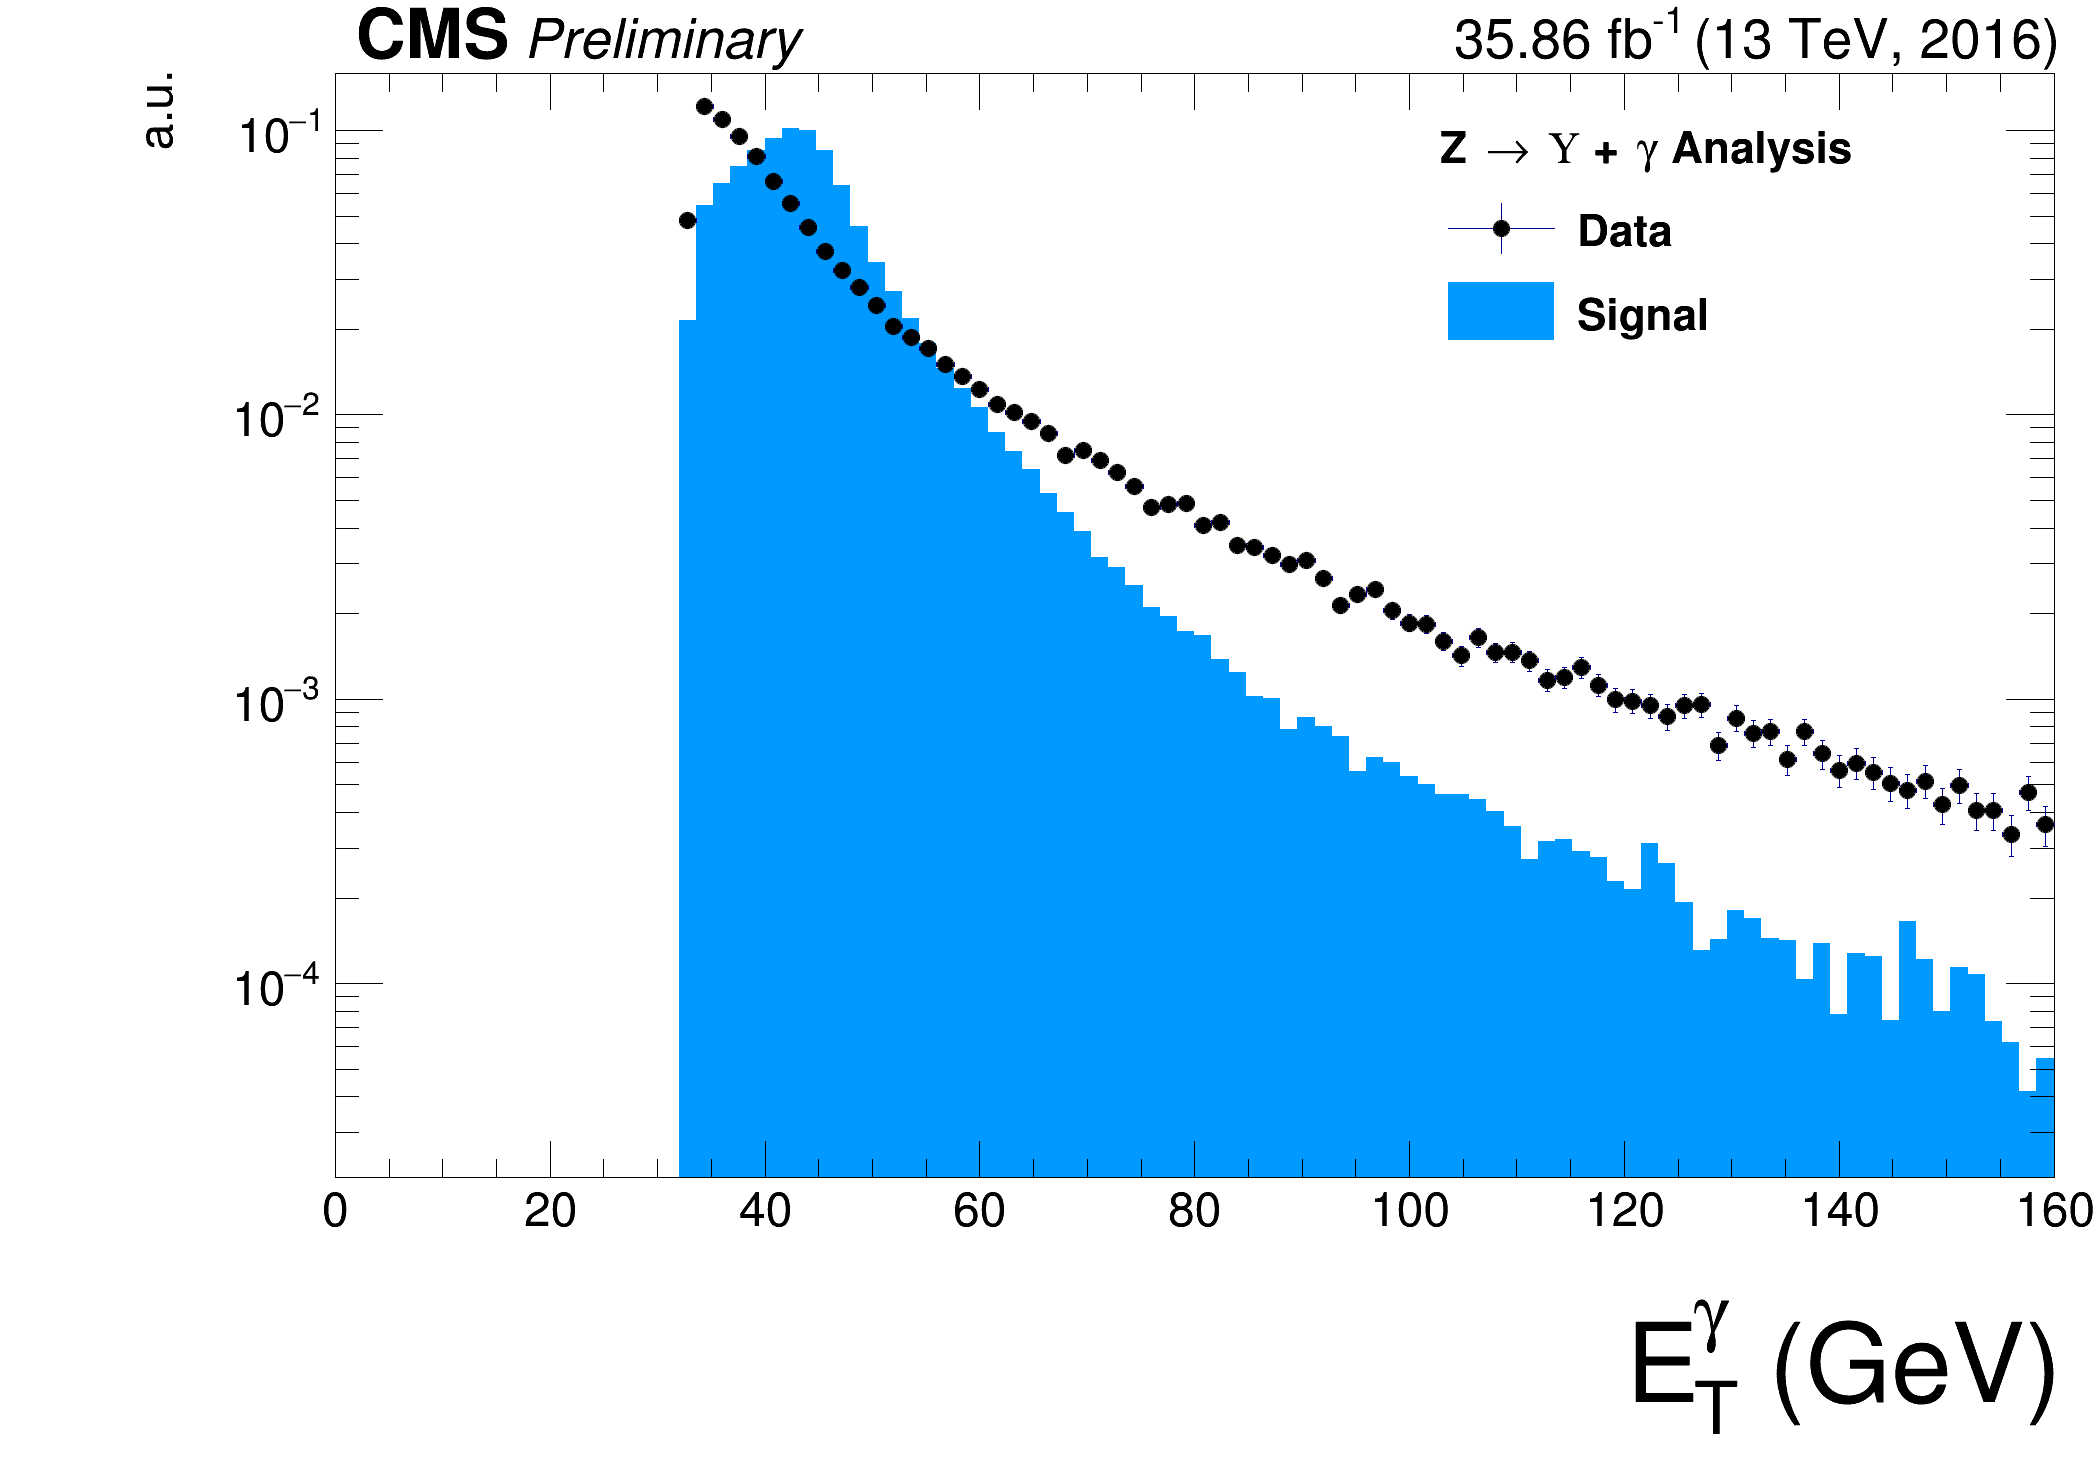
\includegraphics[width=0.45\textwidth]{figures_and_tables/outputPlots/ZtoUpsilon_Cat0_ZZZZZ/au/data_x_mc/noKinCuts/h_noKin_Photon_pt}\hspace*{1.cm}
\end{center}\vspace*{-.5cm}
\caption{The \PT photon distributions from data and signal events for Z decaying into $\Upsilon(1S,2S,3S)$ + $\gamma$ Group I of selection cuts. The plots normalized to the unit of area.}
\label{fig:pTPhoton_ZtoUpsilon_Cat0}
\end{figure}


%%%%%%%$\eta$ Photon distributions for ZtoUpsilon_Cat0
\begin{figure}[!htbp]
\begin{center}
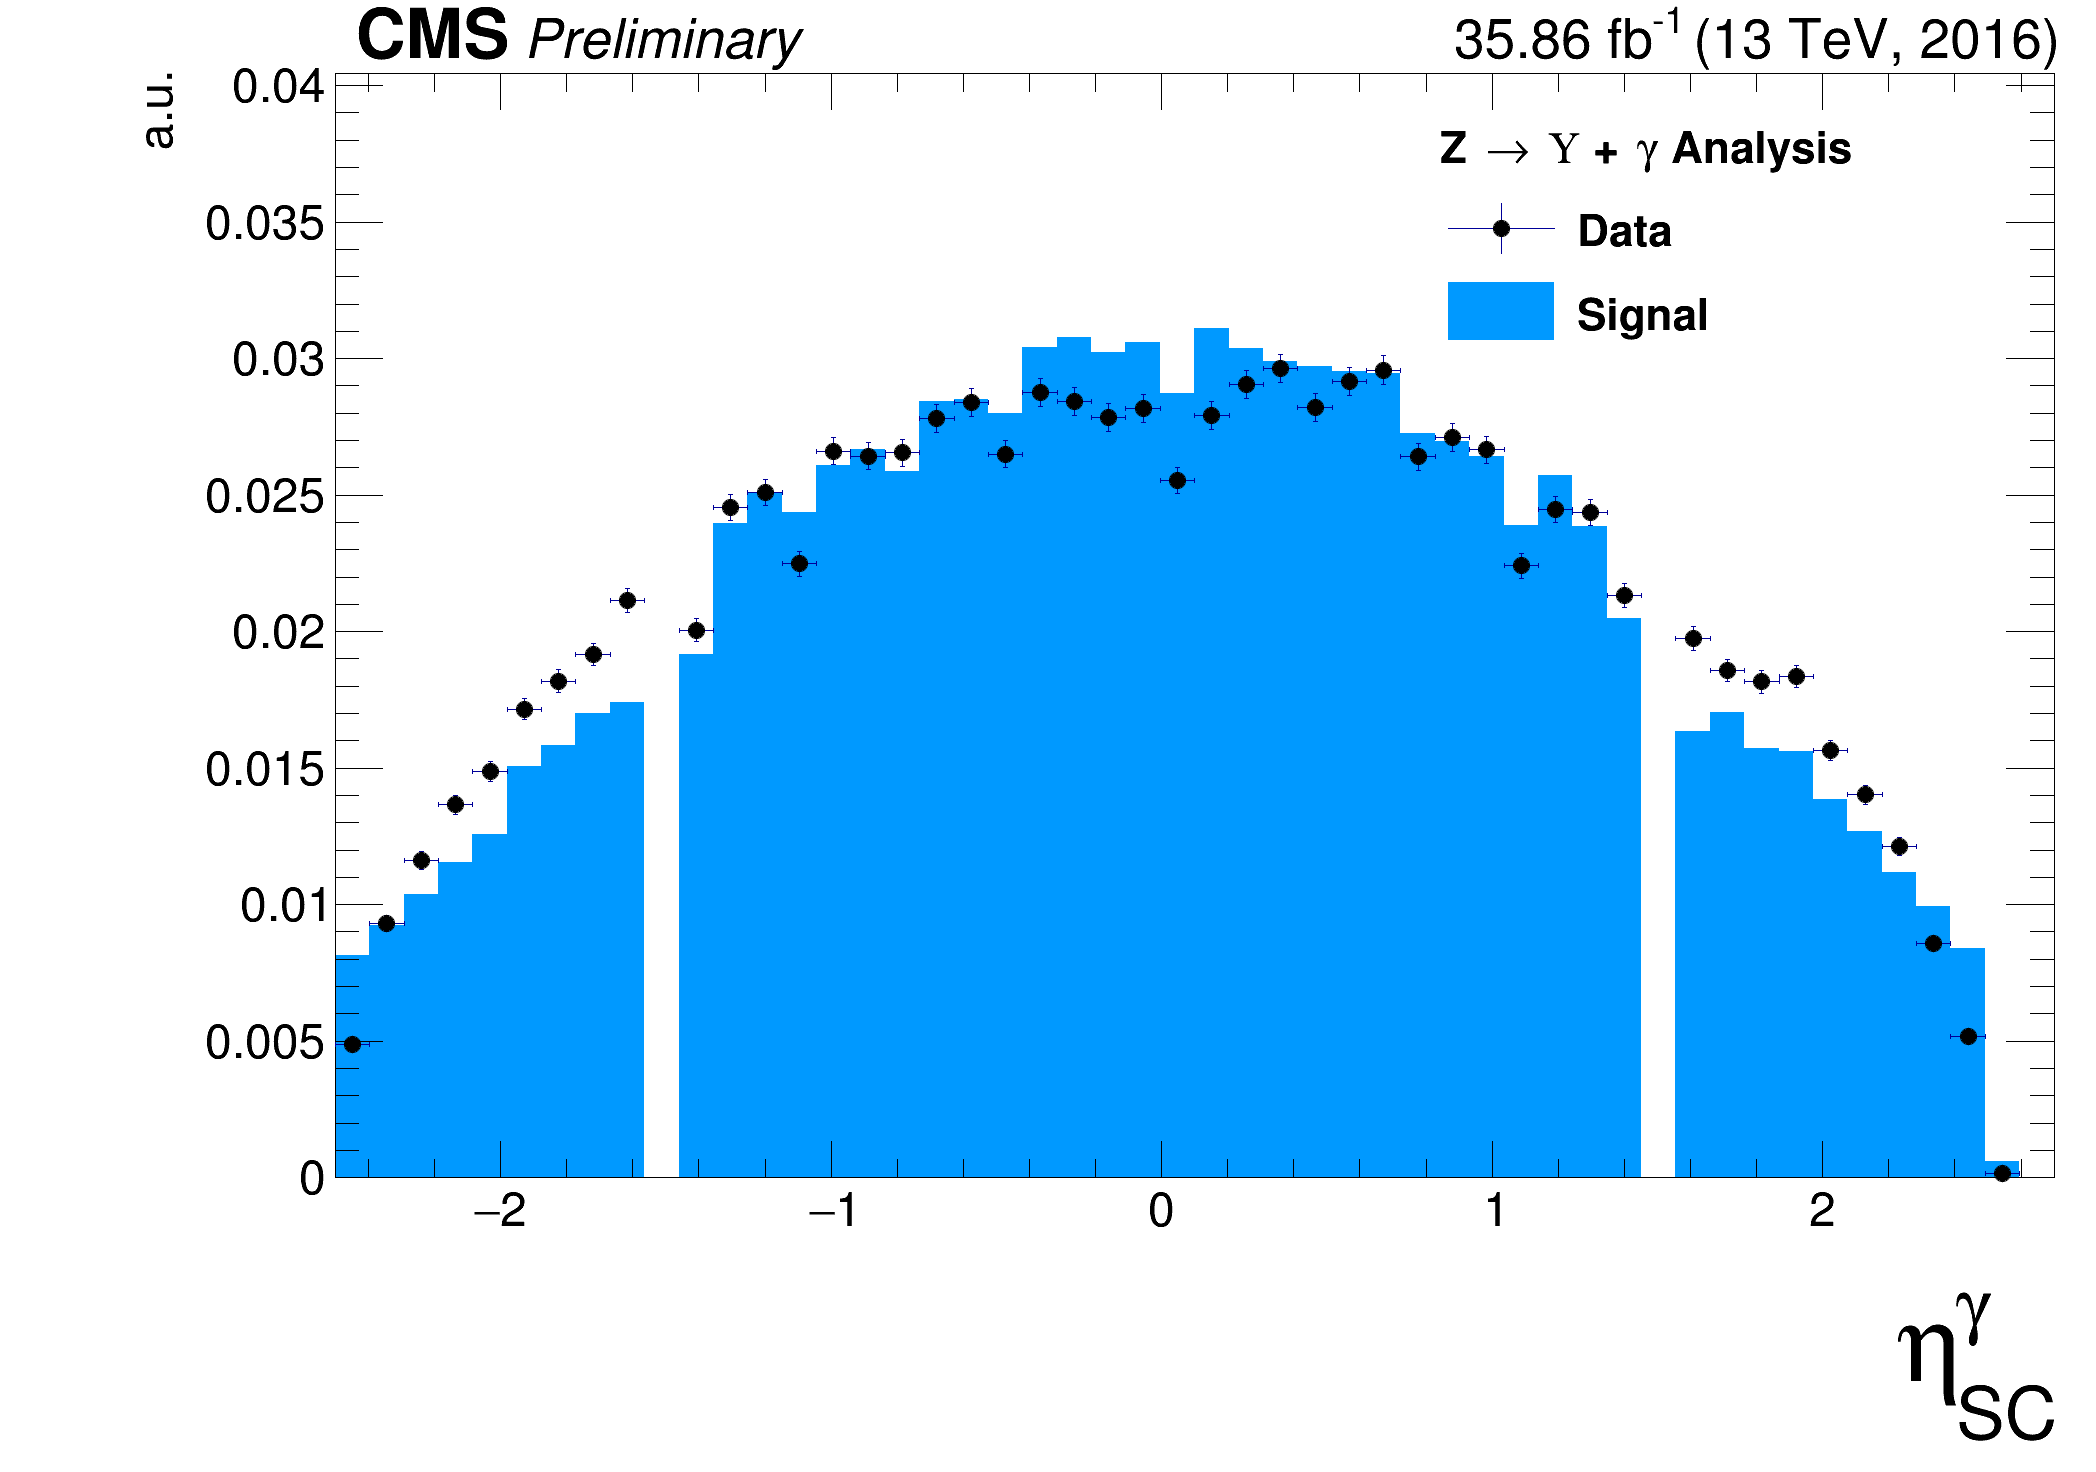
\includegraphics[width=0.45\textwidth]{figures_and_tables/outputPlots/ZtoUpsilon_Cat0_ZZZZZ/au/data_x_mc/noKinCuts/h_noKin_Photon_eta}\hspace*{1.cm}
\end{center}\vspace*{-.5cm}
\caption{The $\eta$ photon distributions from data and signal events of Z decaying into $\Upsilon(1S,2S,3S)$ + $\gamma$ after Group I of selection cuts. The plot is normalized to the unit of area.}
\label{fig:etaPhoton_ZtoUpsilon_Cat0}
\end{figure}

%%%%%%%%% $\phi$ Photon distributions for ZtoUpsilon_Cat0
\begin{figure}[!htbp]
\begin{center}
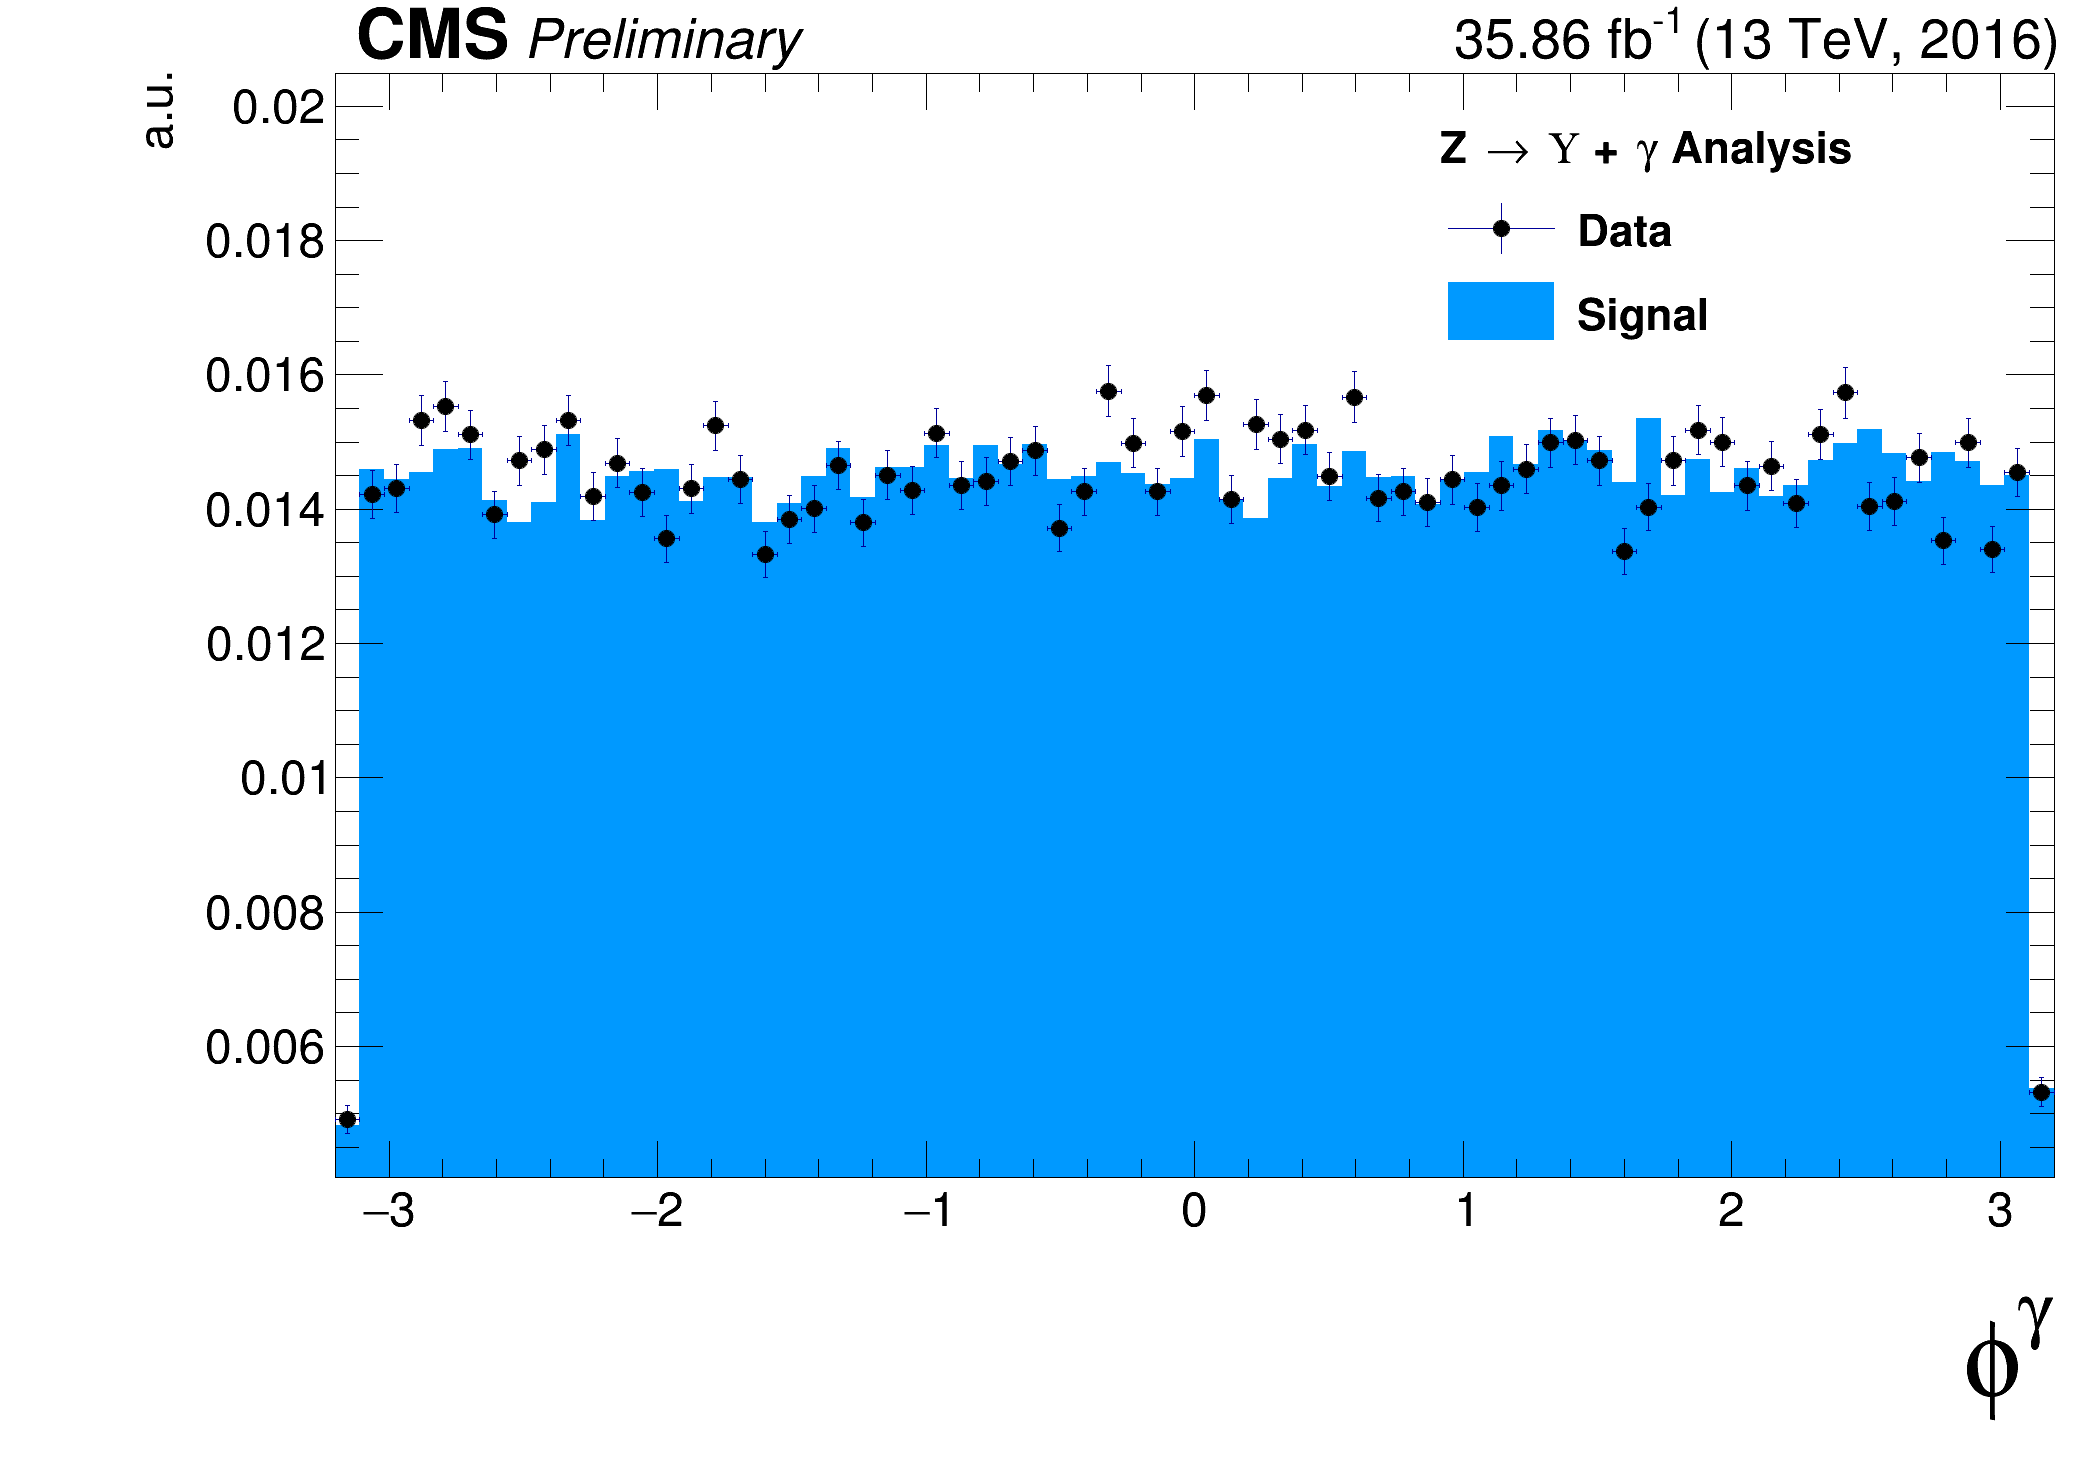
\includegraphics[width=0.45\textwidth]{figures_and_tables/outputPlots/ZtoUpsilon_Cat0_ZZZZZ/au/data_x_mc/noKinCuts/h_noKin_Photon_phi}\hspace*{1.cm}
\end{center}\vspace*{-.5cm}
\caption{The $\phi$ photon distributions from data and signal events of Z decaying into $\Upsilon(1S,2S,3S)$ + $\gamma$ after Group I of selection cuts. The plot is normalized to the unit of area.}
\label{fig:phiPhoton_ZtoUpsilon_Cat0}
\end{figure}

%%%%%%%%%%%%%
% Upsilon and Z boson
%%$\pT$ Upsilon_and_Higgs distributions for ZtoUpsilon_Cat0
\begin{figure}[!htbp]
\begin{center}
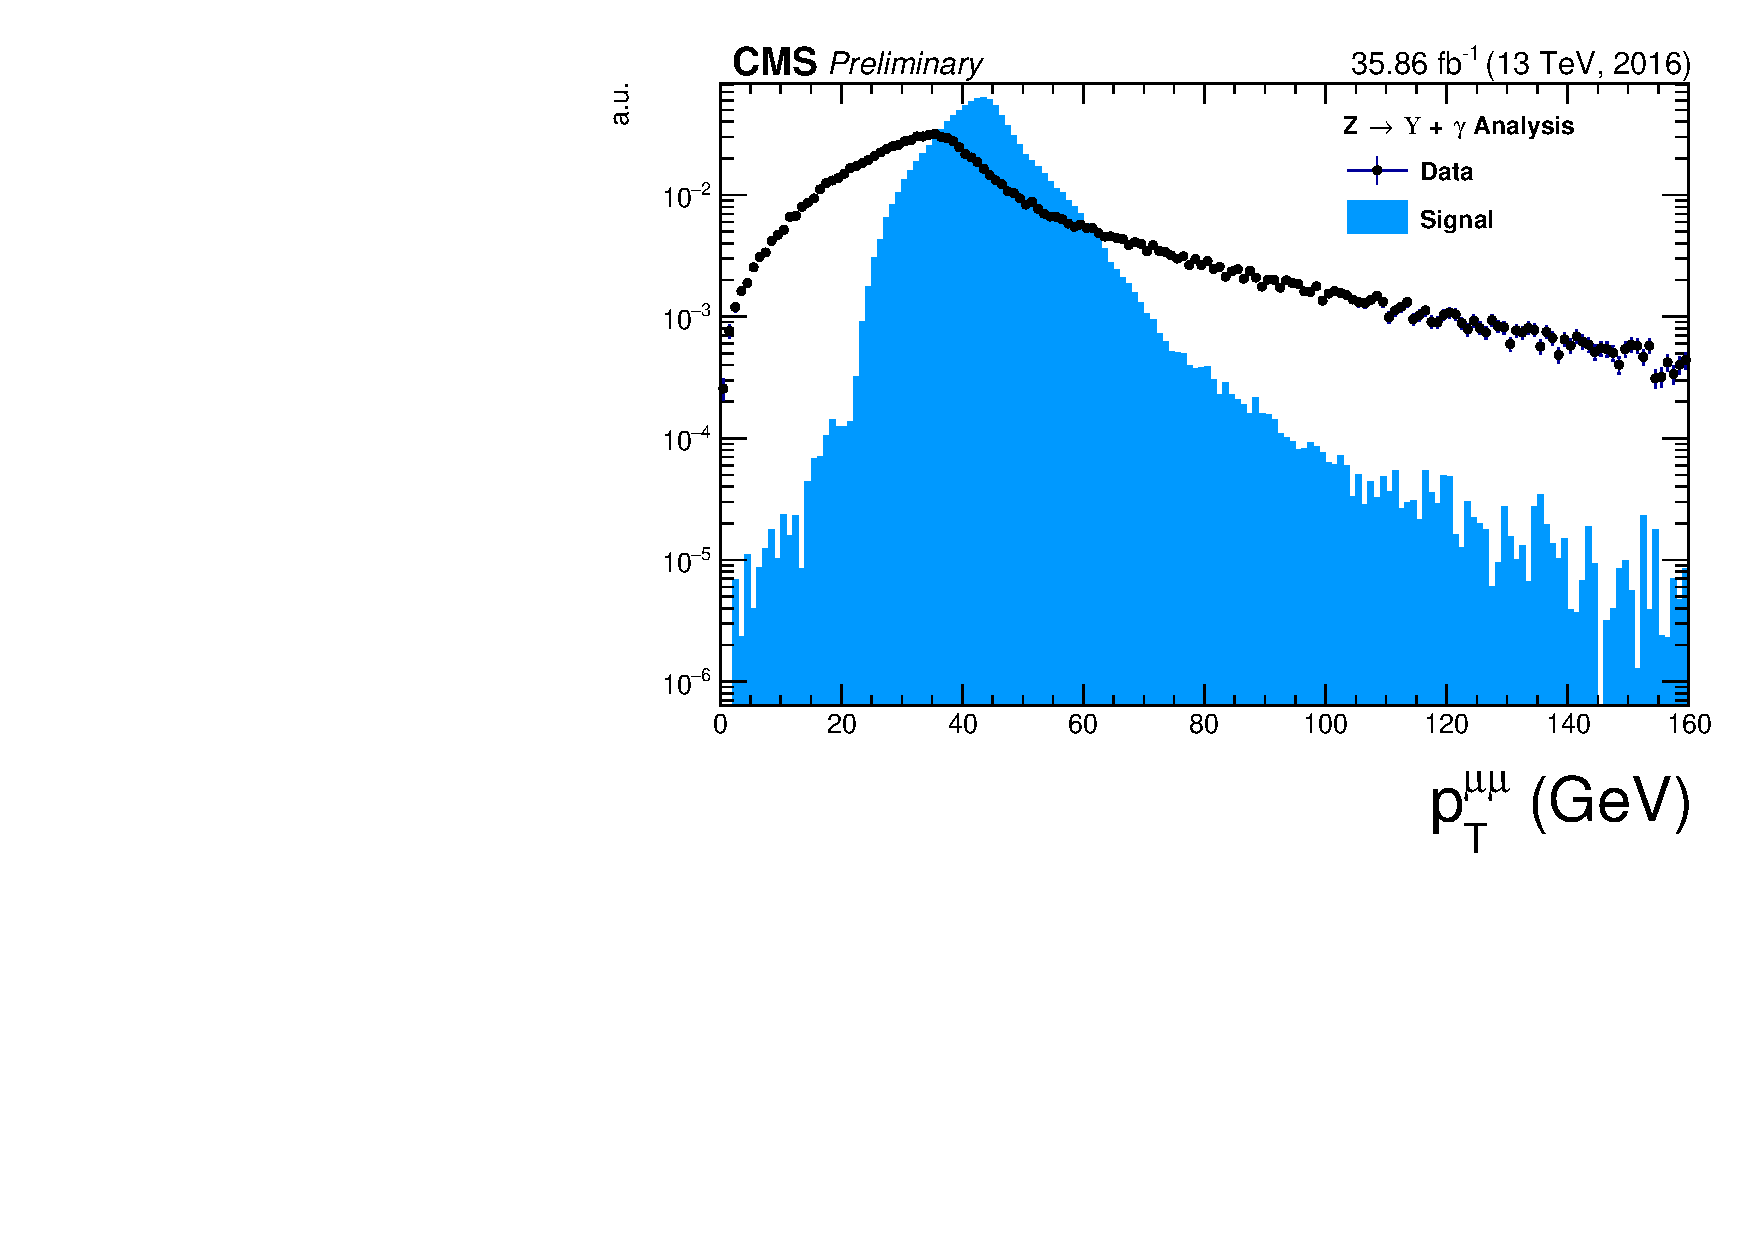
\includegraphics[width=0.45\textwidth]{figures_and_tables/outputPlots/ZtoUpsilon_Cat0_ZZZZZ/au/data_x_mc/noKinCuts/h_noKin_Upsilon_Pt}\hspace*{1.cm}
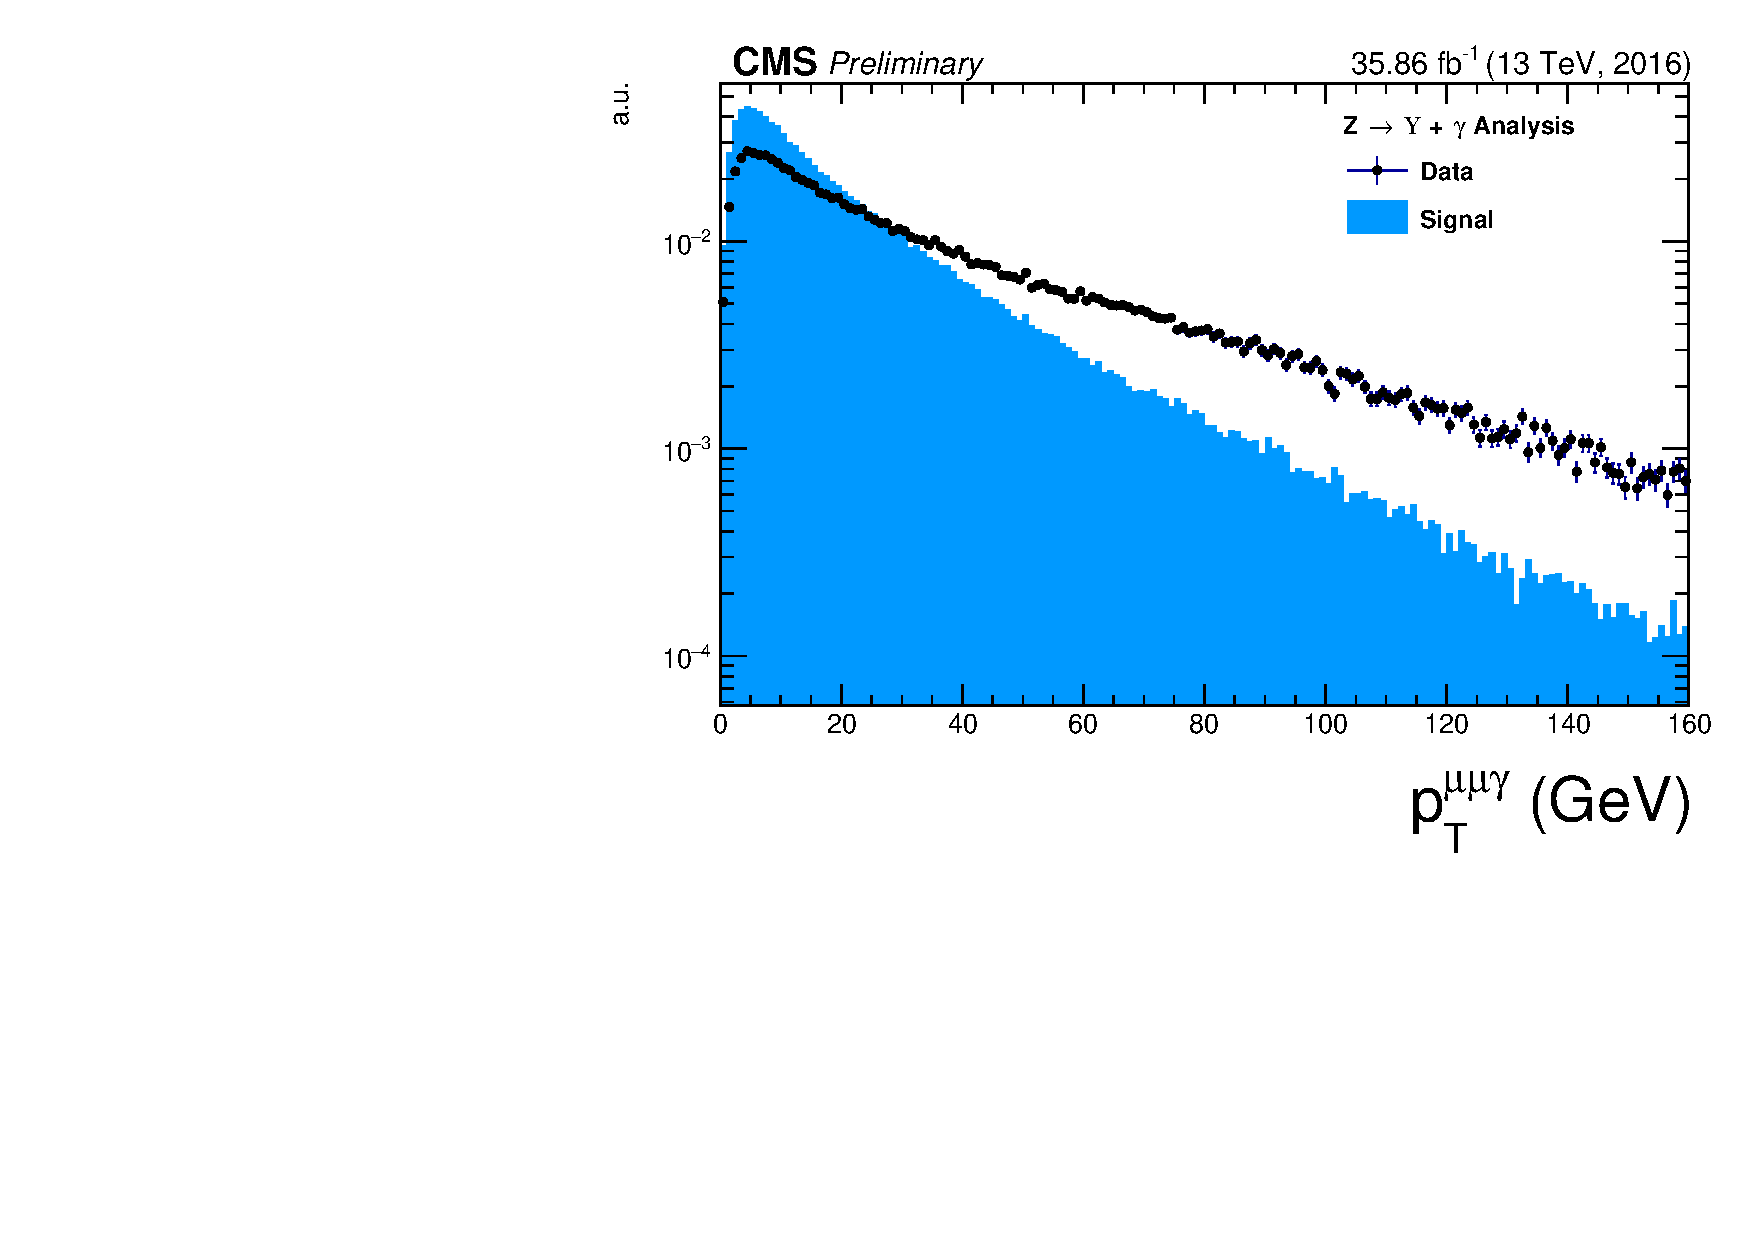
\includegraphics[width=0.45\textwidth]{figures_and_tables/outputPlots/ZtoUpsilon_Cat0_ZZZZZ/au/data_x_mc/noKinCuts/h_noKin_Z_Pt}
\end{center}\vspace*{-.5cm}
\caption{The \PT distributions for the reconstructed $\Upsilon(1S,2S,3S)$ in the left and for Z in the right from data and signal events for Z decaying into $\Upsilon(1S,2S,3S)$ + $\gamma$ after Group I of selection cuts. The plots are normalized to the unit of area. The black dots are data collect by CMS while the blue distribution is related only to the signal Monte-Carlo generated samples.}
\label{fig:pTUpsilon_and_Z_ZtoUpsilon_Cat0}
\end{figure}


%%%%%%%$\eta$ Upsilon_and_Z distributions for ZtoUpsilon_Cat0
\begin{figure}[!htbp]
\begin{center}
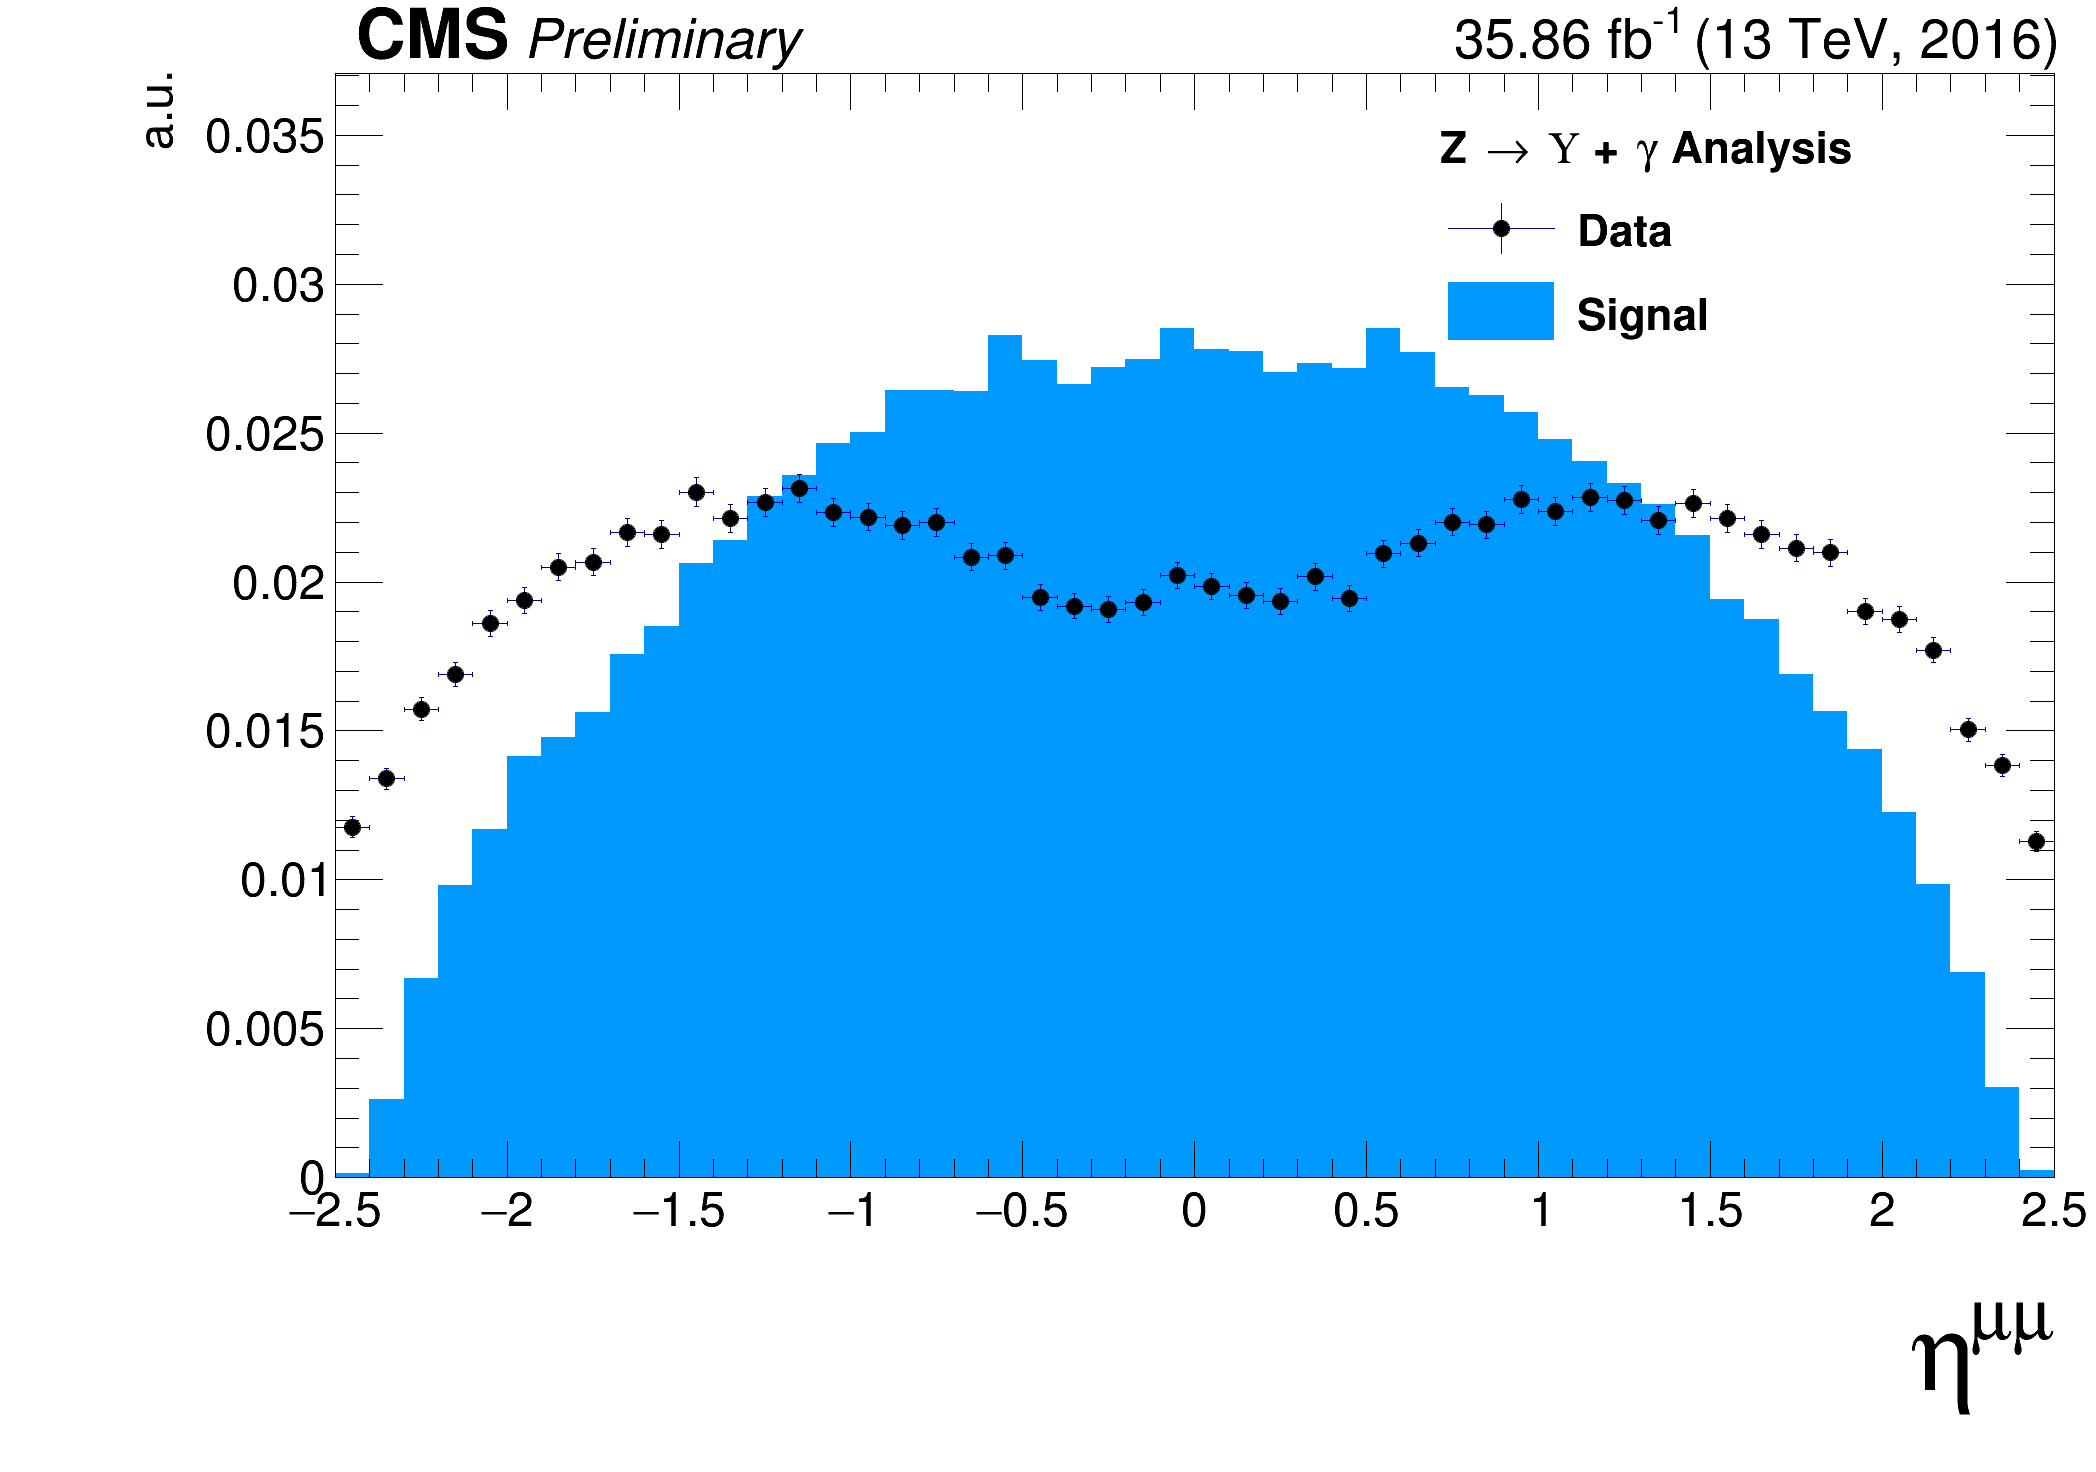
\includegraphics[width=0.45\textwidth]{figures_and_tables/outputPlots/ZtoUpsilon_Cat0_ZZZZZ/au/data_x_mc/noKinCuts/h_noKin_Upsilon_eta}\hspace*{1.cm}
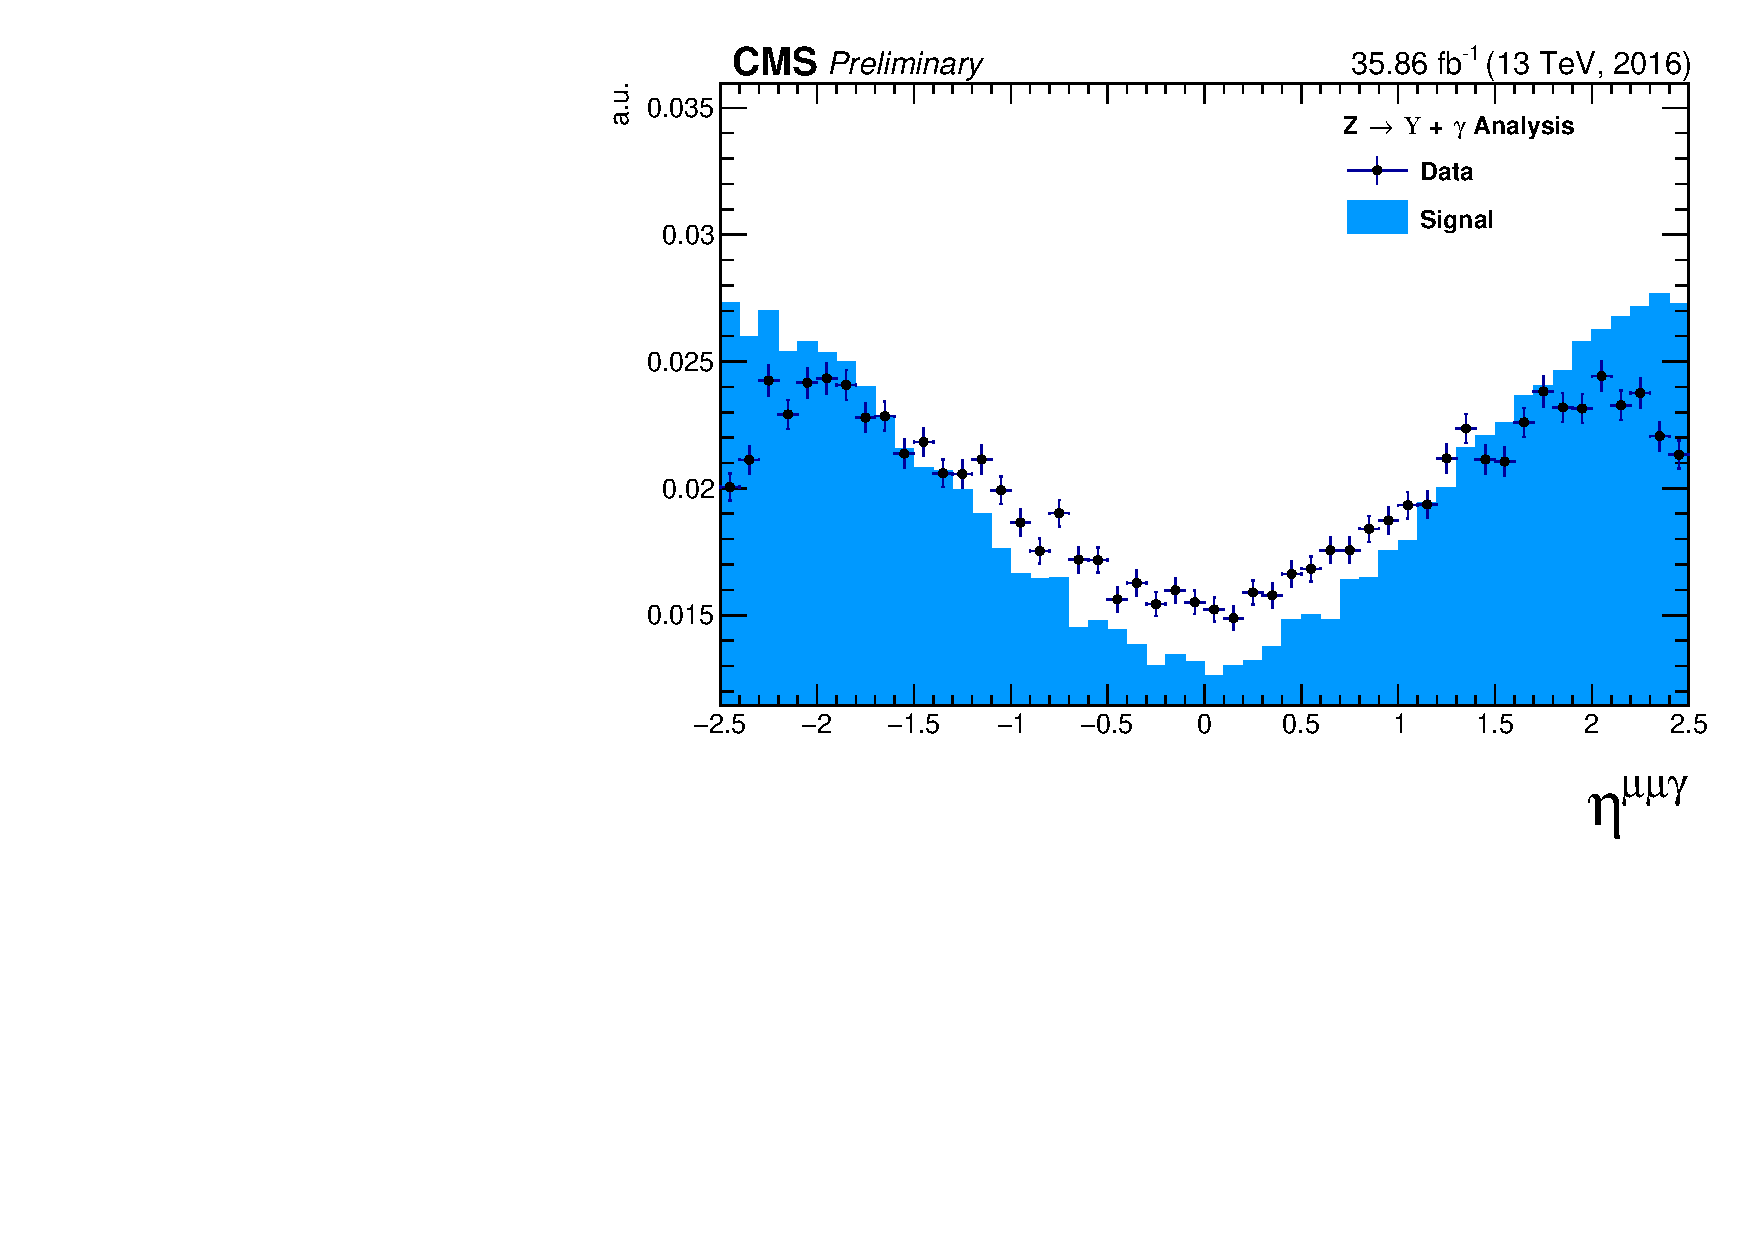
\includegraphics[width=0.45\textwidth]{figures_and_tables/outputPlots/ZtoUpsilon_Cat0_ZZZZZ/au/data_x_mc/noKinCuts/h_noKin_Z_eta}
\end{center}\vspace*{-.5cm}
\caption{The $\eta$ distributions for $\Upsilon(1S,2S,3S)$ in the left and for Z in the right from data and signal events for Z decaying into $\Upsilon(1S,2S,3S)$ + $\gamma$ after Group I of selection cuts. The plots are normalized to the unit of area. The black dots are data collect by CMS while the blue distribution is related only to the signal Monte-Carlo generated samples.}
\label{fig:etaUpsilon_and_Z_ZtoUpsilon_Cat0}
\end{figure}

%%%%%%%%% $\phi$ Upsilon_and_Zdistributions for ZtoUpsilon_Cat0
\begin{figure}[!htbp]
\begin{center}
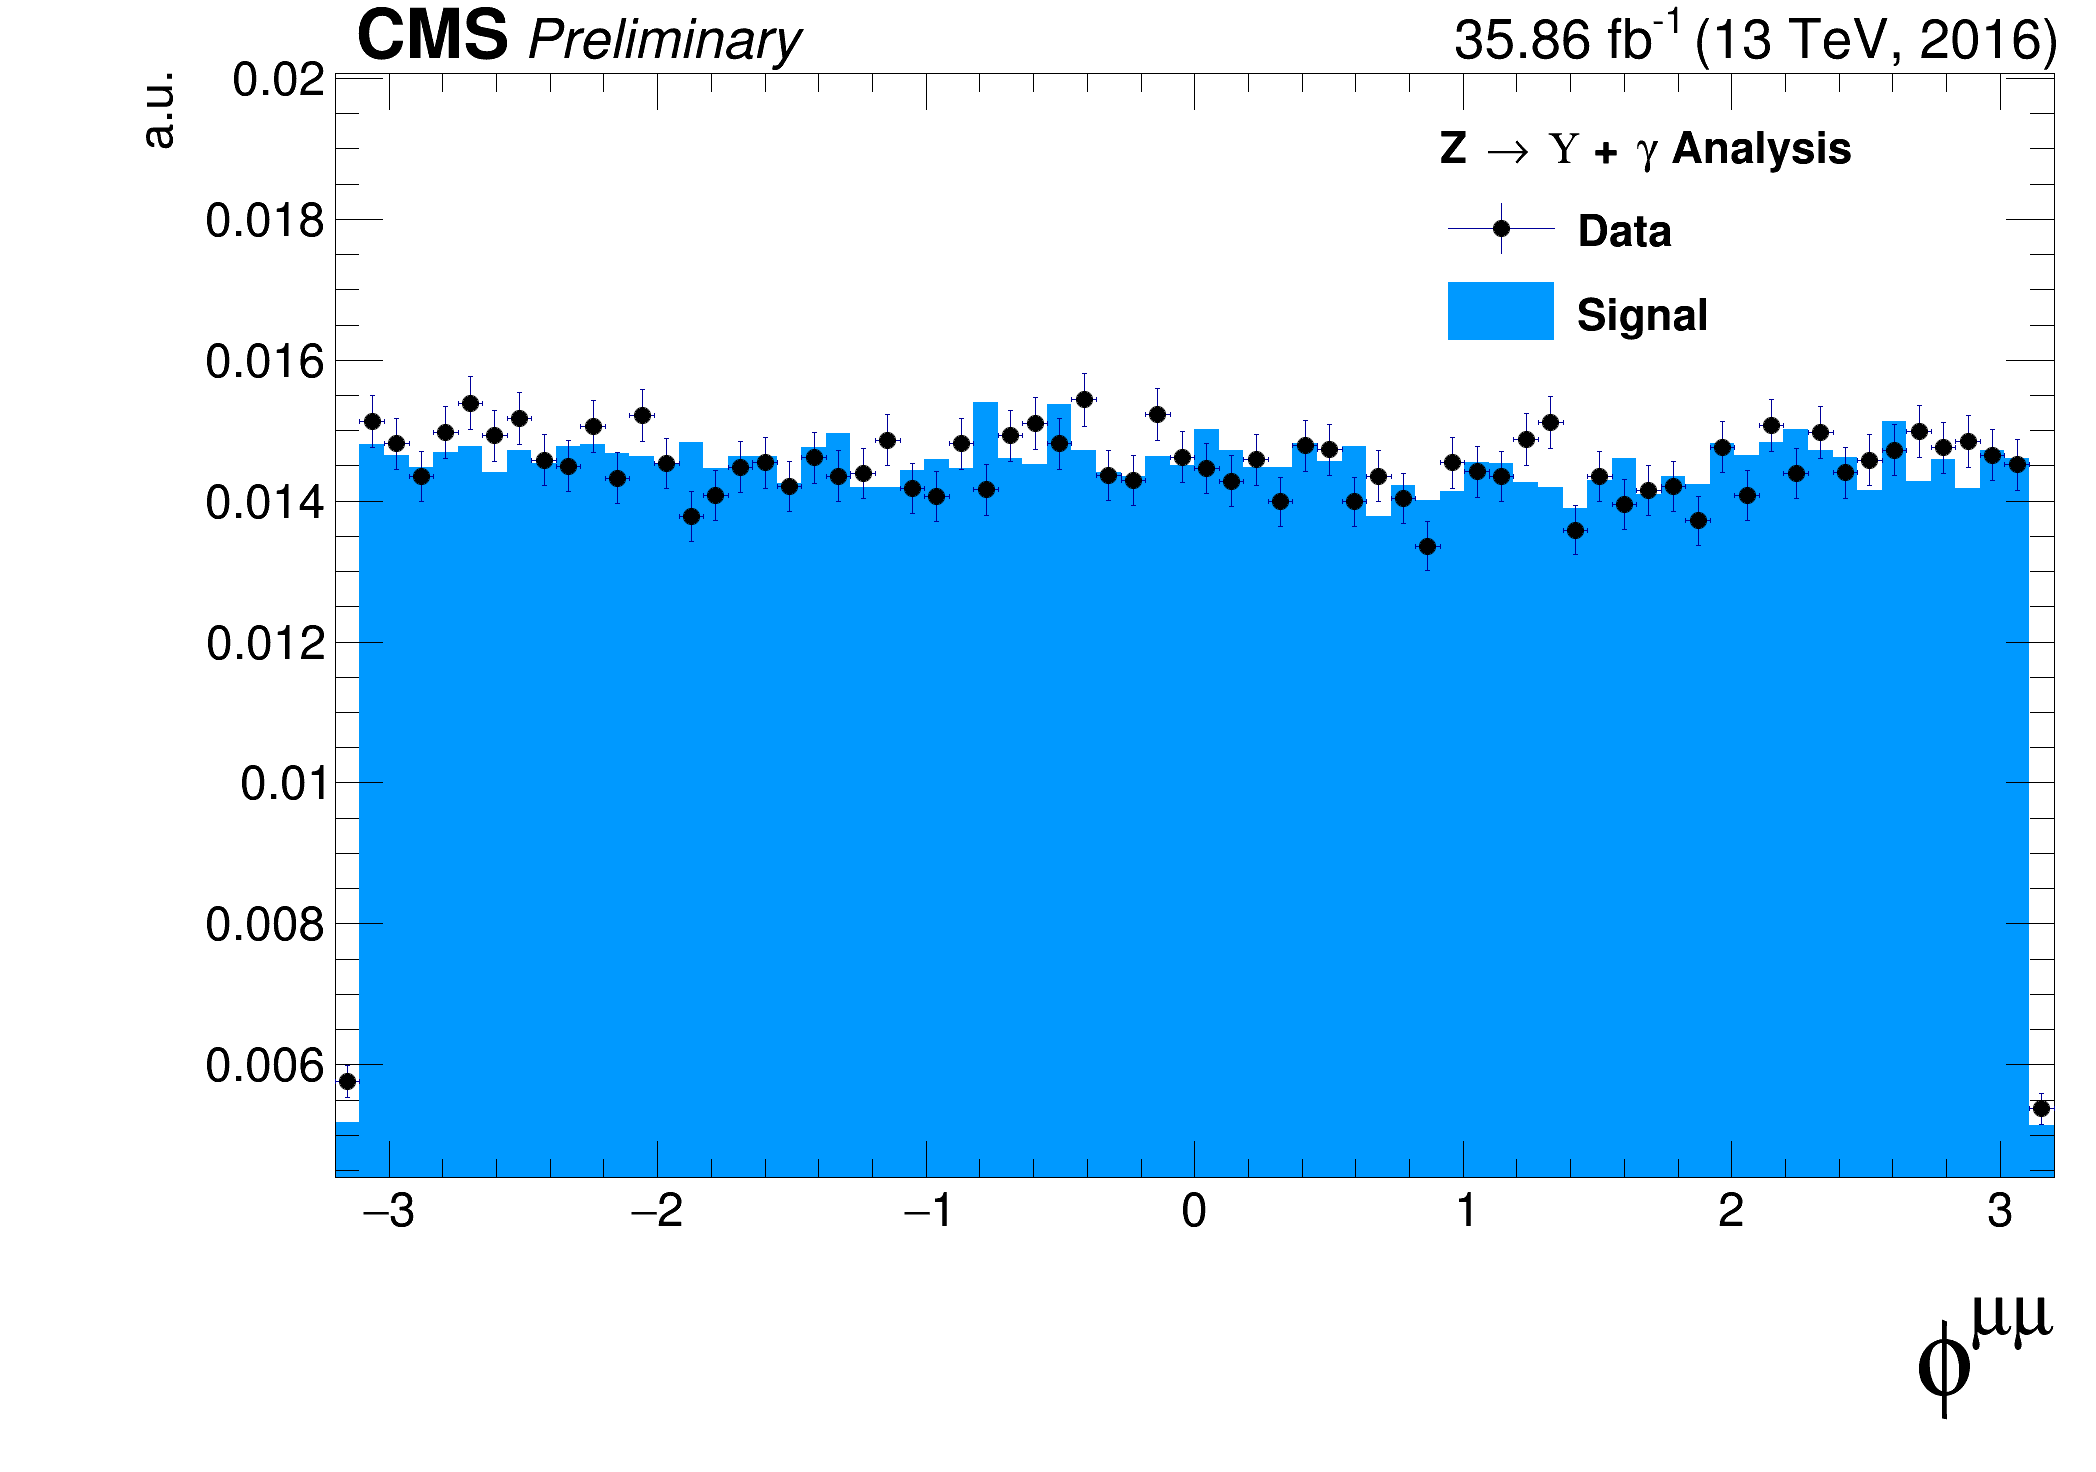
\includegraphics[width=0.45\textwidth]{figures_and_tables/outputPlots/ZtoUpsilon_Cat0_ZZZZZ/au/data_x_mc/noKinCuts/h_noKin_Upsilon_phi}\hspace*{1.cm}
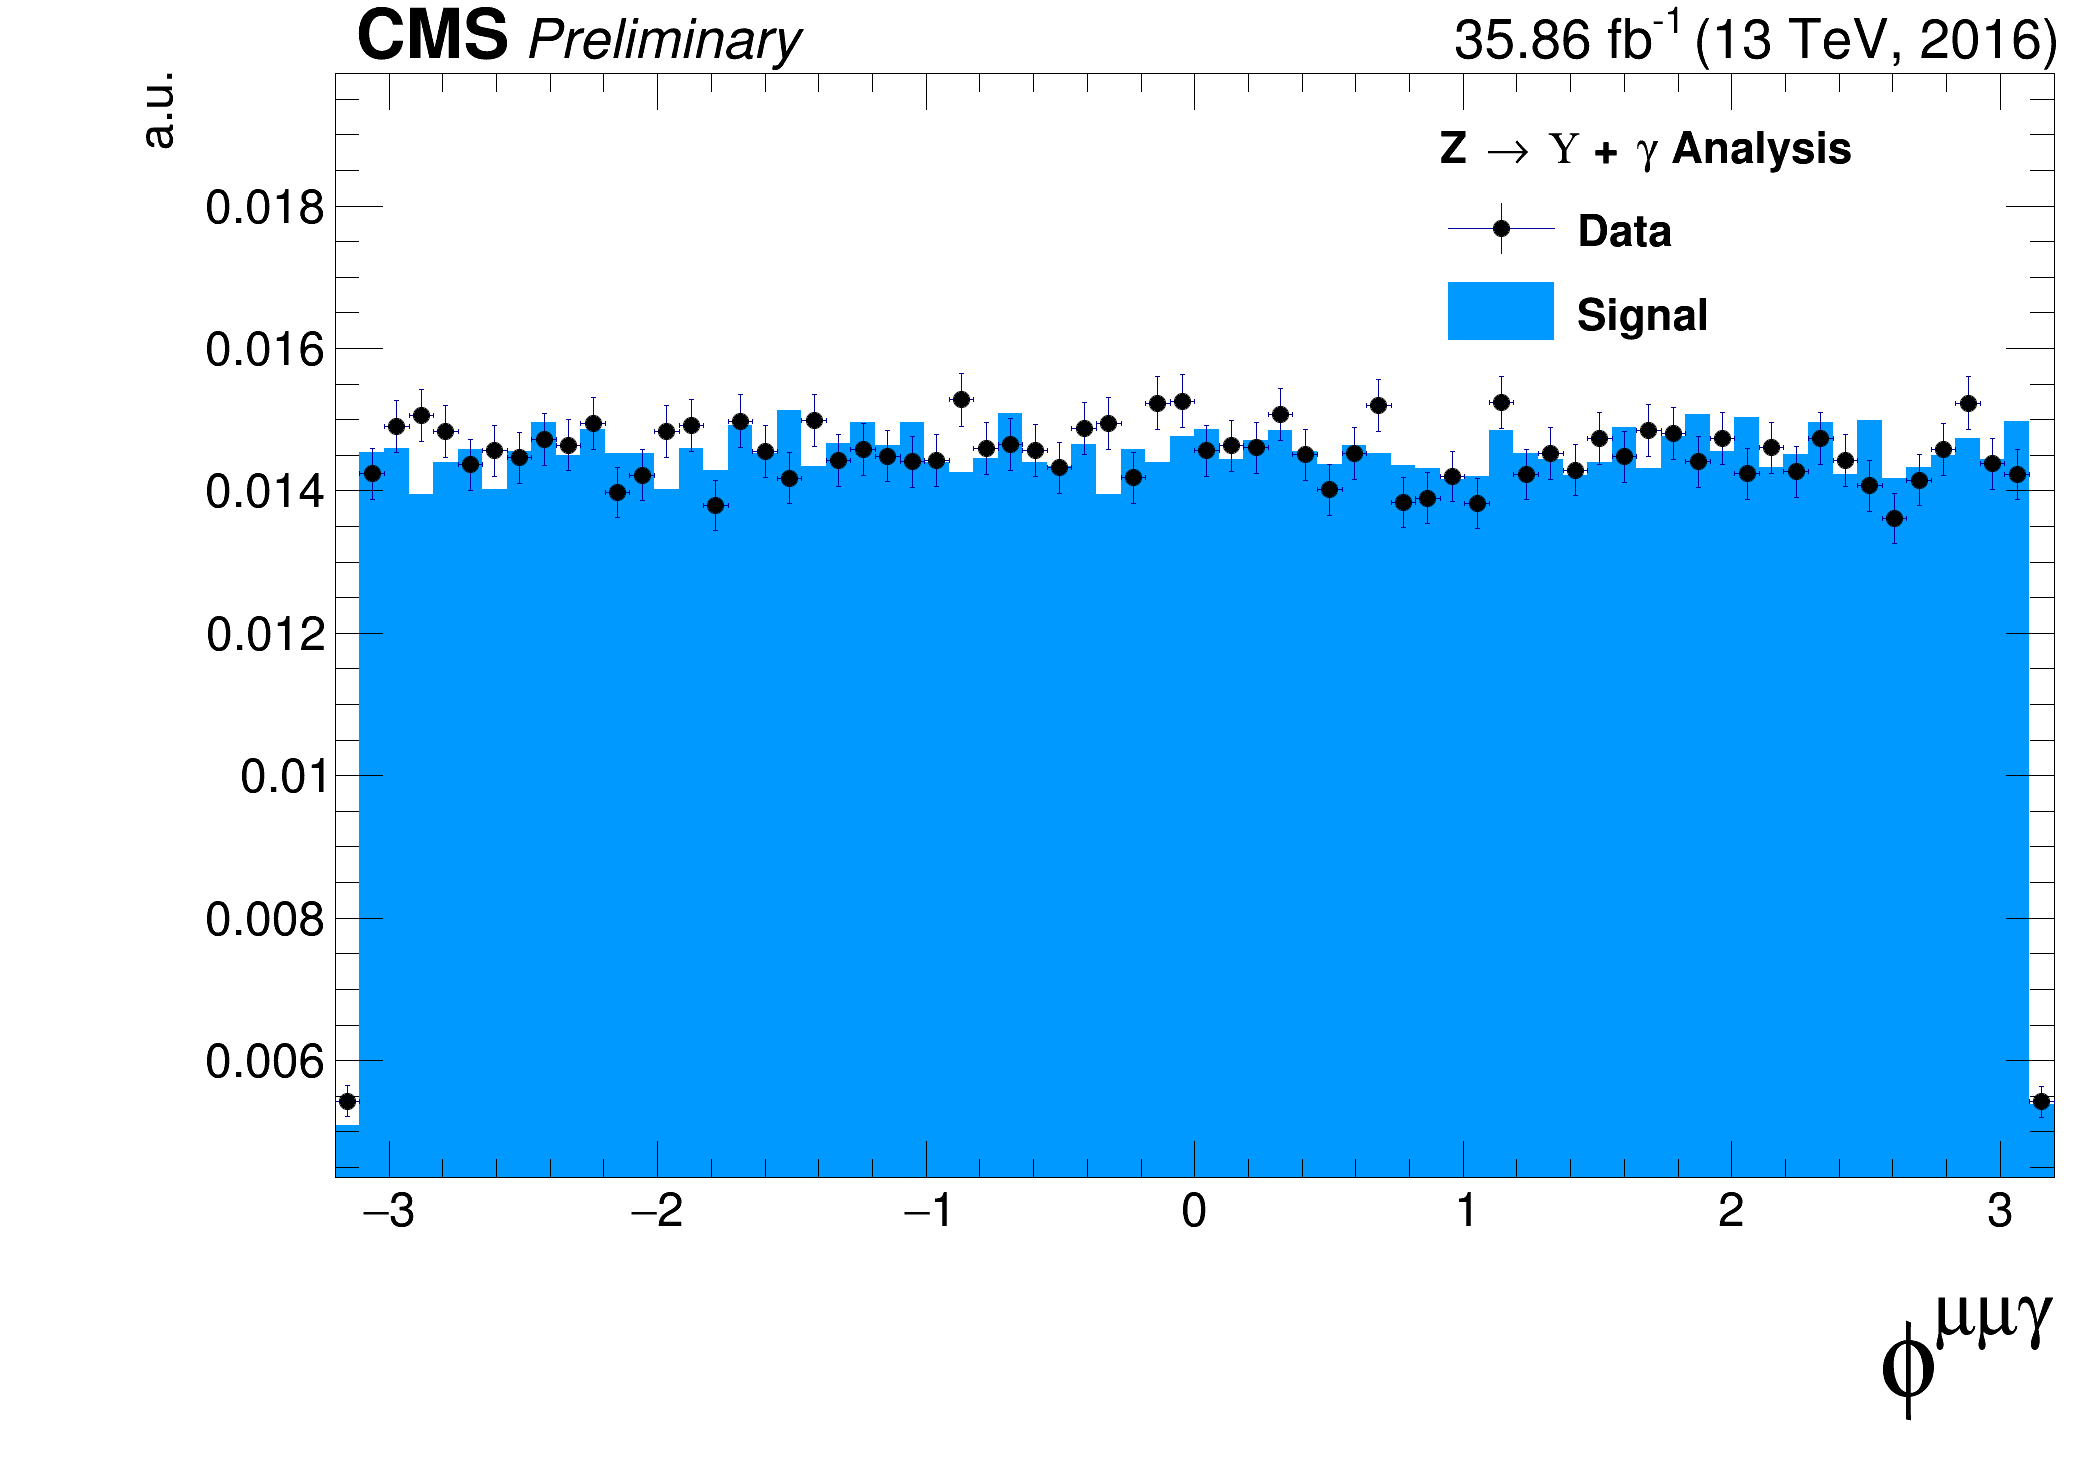
\includegraphics[width=0.45\textwidth]{figures_and_tables/outputPlots/ZtoUpsilon_Cat0_ZZZZZ/au/data_x_mc/noKinCuts/h_noKin_Z_phi}
\end{center}\vspace*{-.5cm}
\caption{The $\phi$ distributions for $\Upsilon(1S,2S,3S)$ in the left and for Z in the right from data and signal events for Z decaying into $\Upsilon(1S,2S,3S)$ + $\gamma$ after Group I of selection cuts. The plots are normalized to the unit of area. The black dots are data collect by CMS while the blue distribution is related only to the signal Monte-Carlo generated samples.}
\label{fig:phiUpsilon_and_Z_ZtoUpsilon_Cat0}
\end{figure}

%%%%%%%%%%%%

%%%%%%%%%%%%%
% kin cuts
%% delta R -  mu x photon distributions for ZtoUpsilon_Cat0
\begin{figure}[!htbp]
\begin{center}
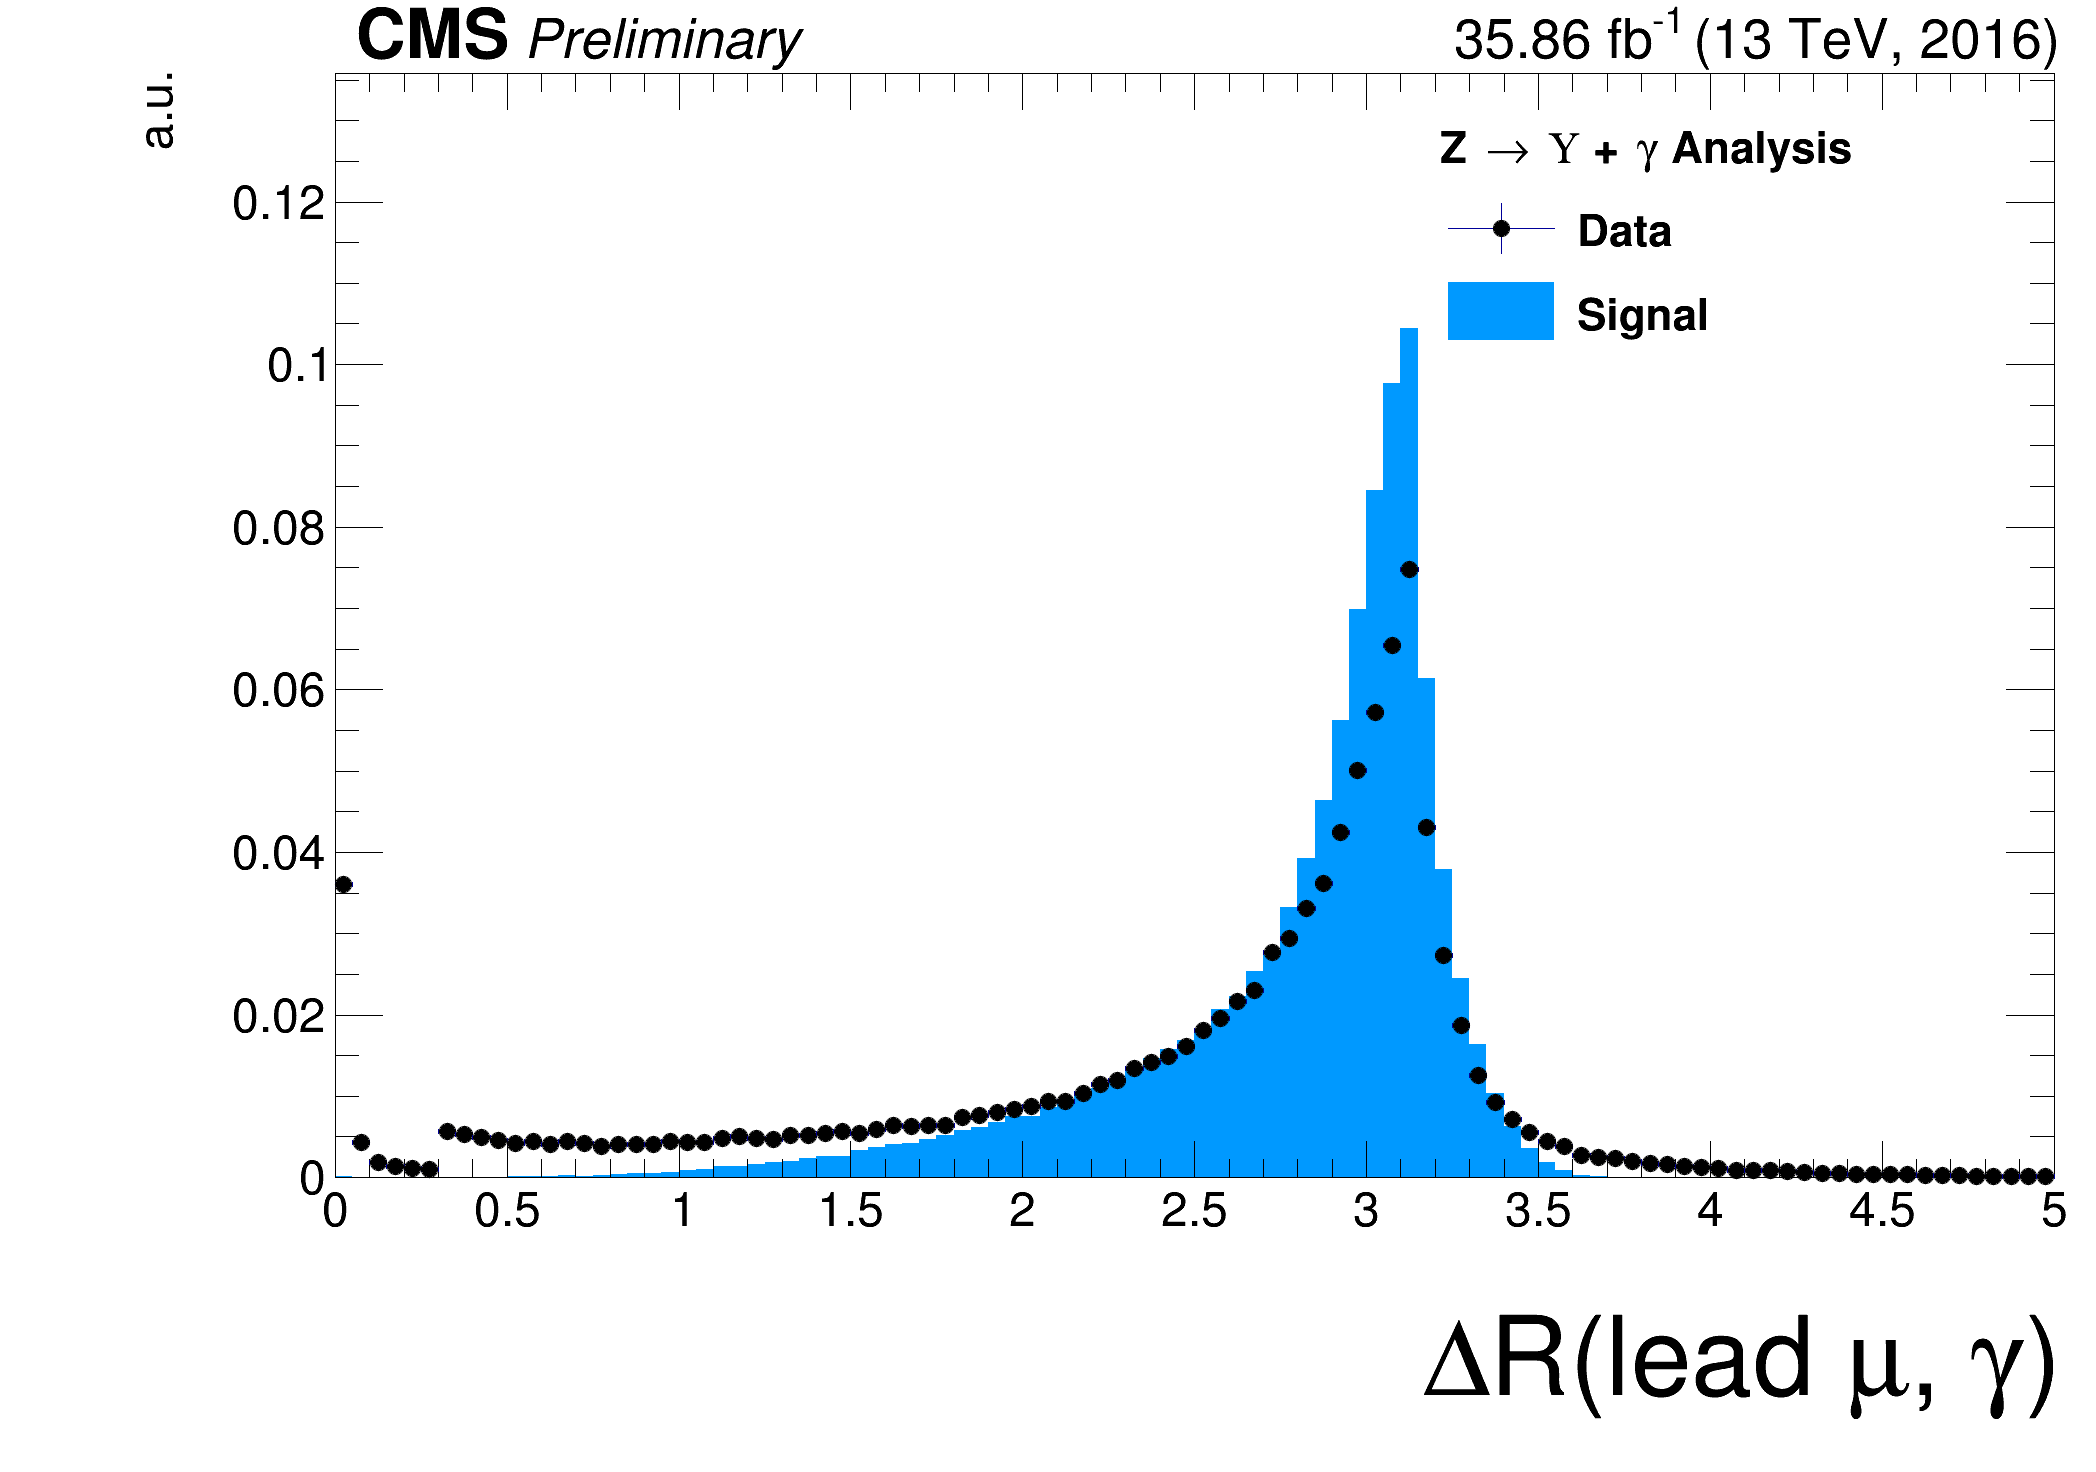
\includegraphics[width=0.45\textwidth]{figures_and_tables/outputPlots/ZtoUpsilon_Cat0_ZZZZZ/au/data_x_mc/noKinCuts/h_noKin_deltaR_Leading_Photon}\hspace*{1.cm}
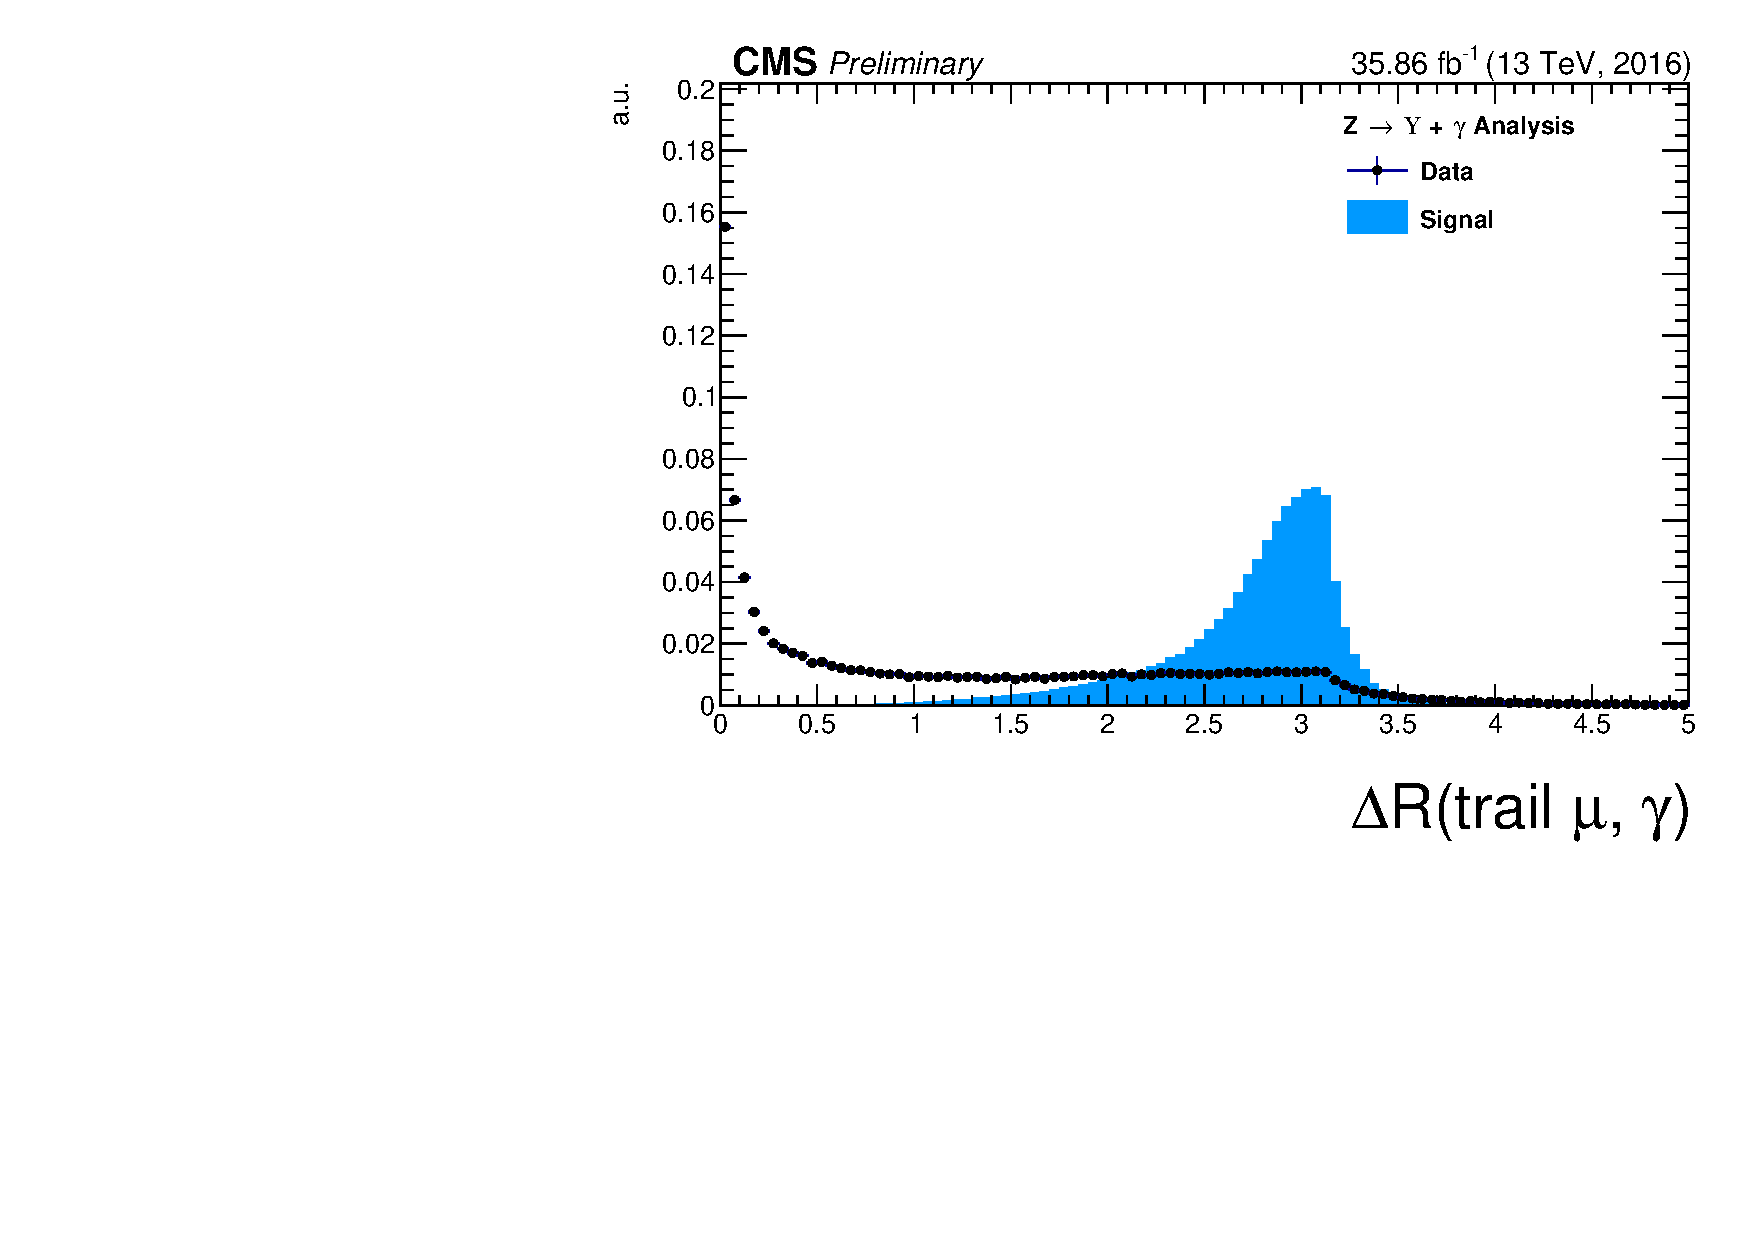
\includegraphics[width=0.45\textwidth]{figures_and_tables/outputPlots/ZtoUpsilon_Cat0_ZZZZZ/au/data_x_mc/noKinCuts/h_noKin_deltaR_Trailing_Photon}\end{center}\vspace*{-.5cm}
\caption{The $\Delta R$ distributions between the photon and the leading muon (left) and the trailing muon (right) for for Z decaying into $\Upsilon(1S,2S,3S)$ + $\gamma$ from data and signal events after Group I of selection cuts. The plots are normalized to the unit of area. The black dots are data collect by CMS while the blue distribution is related only to the signal Monte-Carlo generated samples.}
\label{fig:deltaR_ZtoUpsilon_Cat0}
\end{figure}

%% delta R and Delta Phi -  MuMu x photon distributions for ZtoUpsilon_Cat0
\begin{figure}[!htbp]
\begin{center}
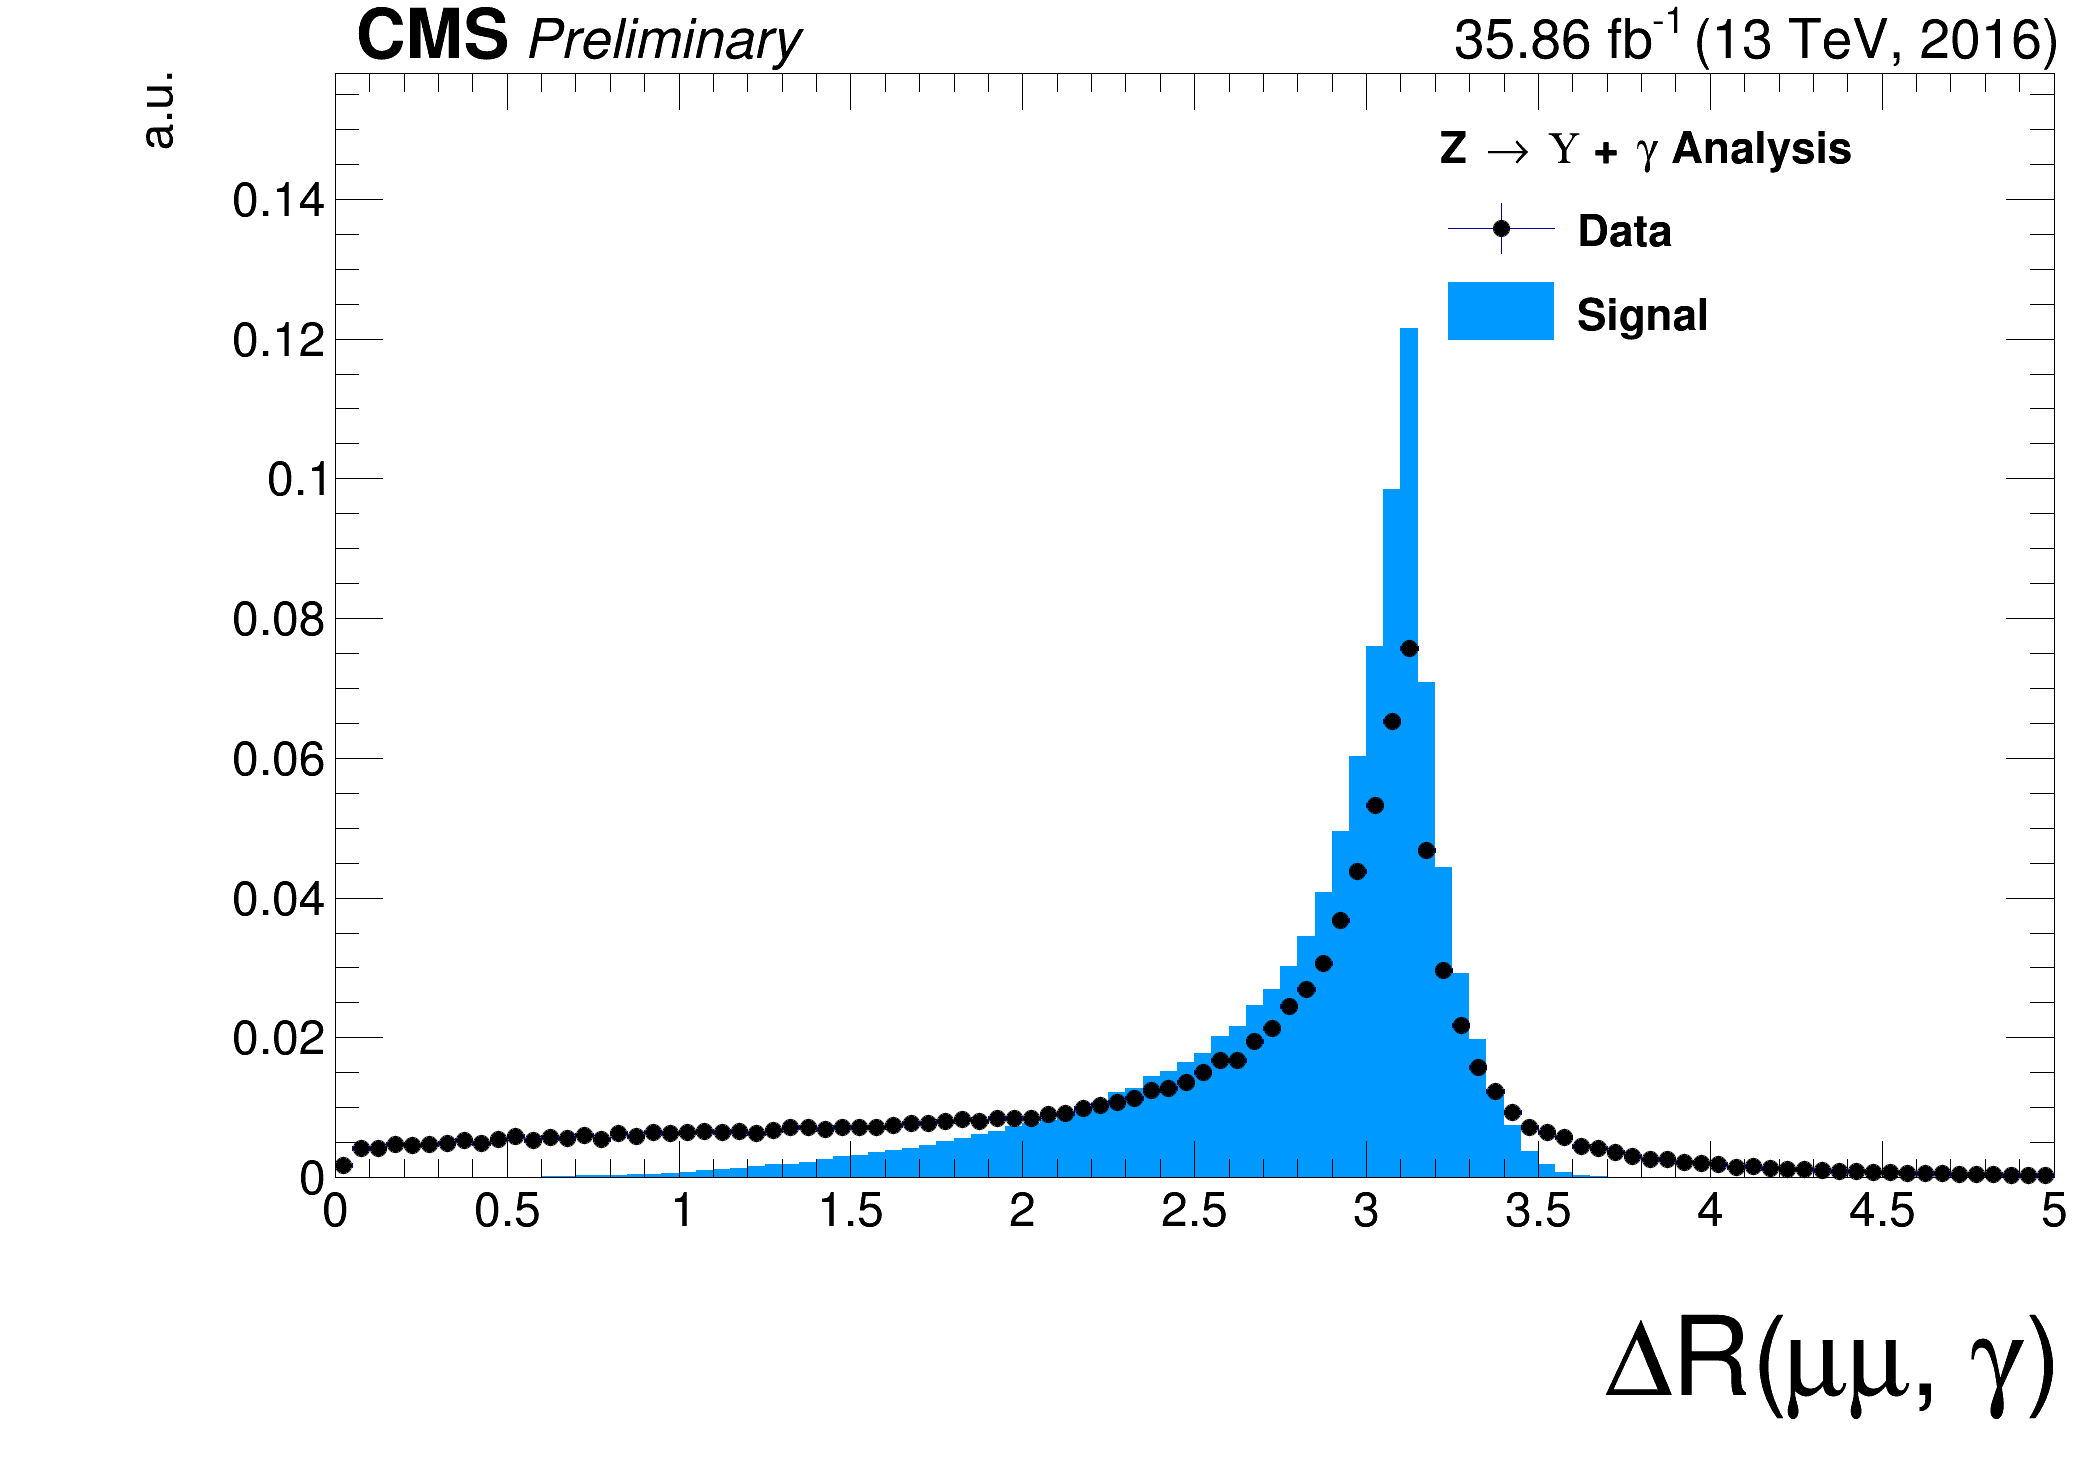
\includegraphics[width=0.45\textwidth]{figures_and_tables/outputPlots/ZtoUpsilon_Cat0_ZZZZZ/au/data_x_mc/noKinCuts/h_noKin_deltaR_Upsilon_Photon}\hspace*{1.cm}
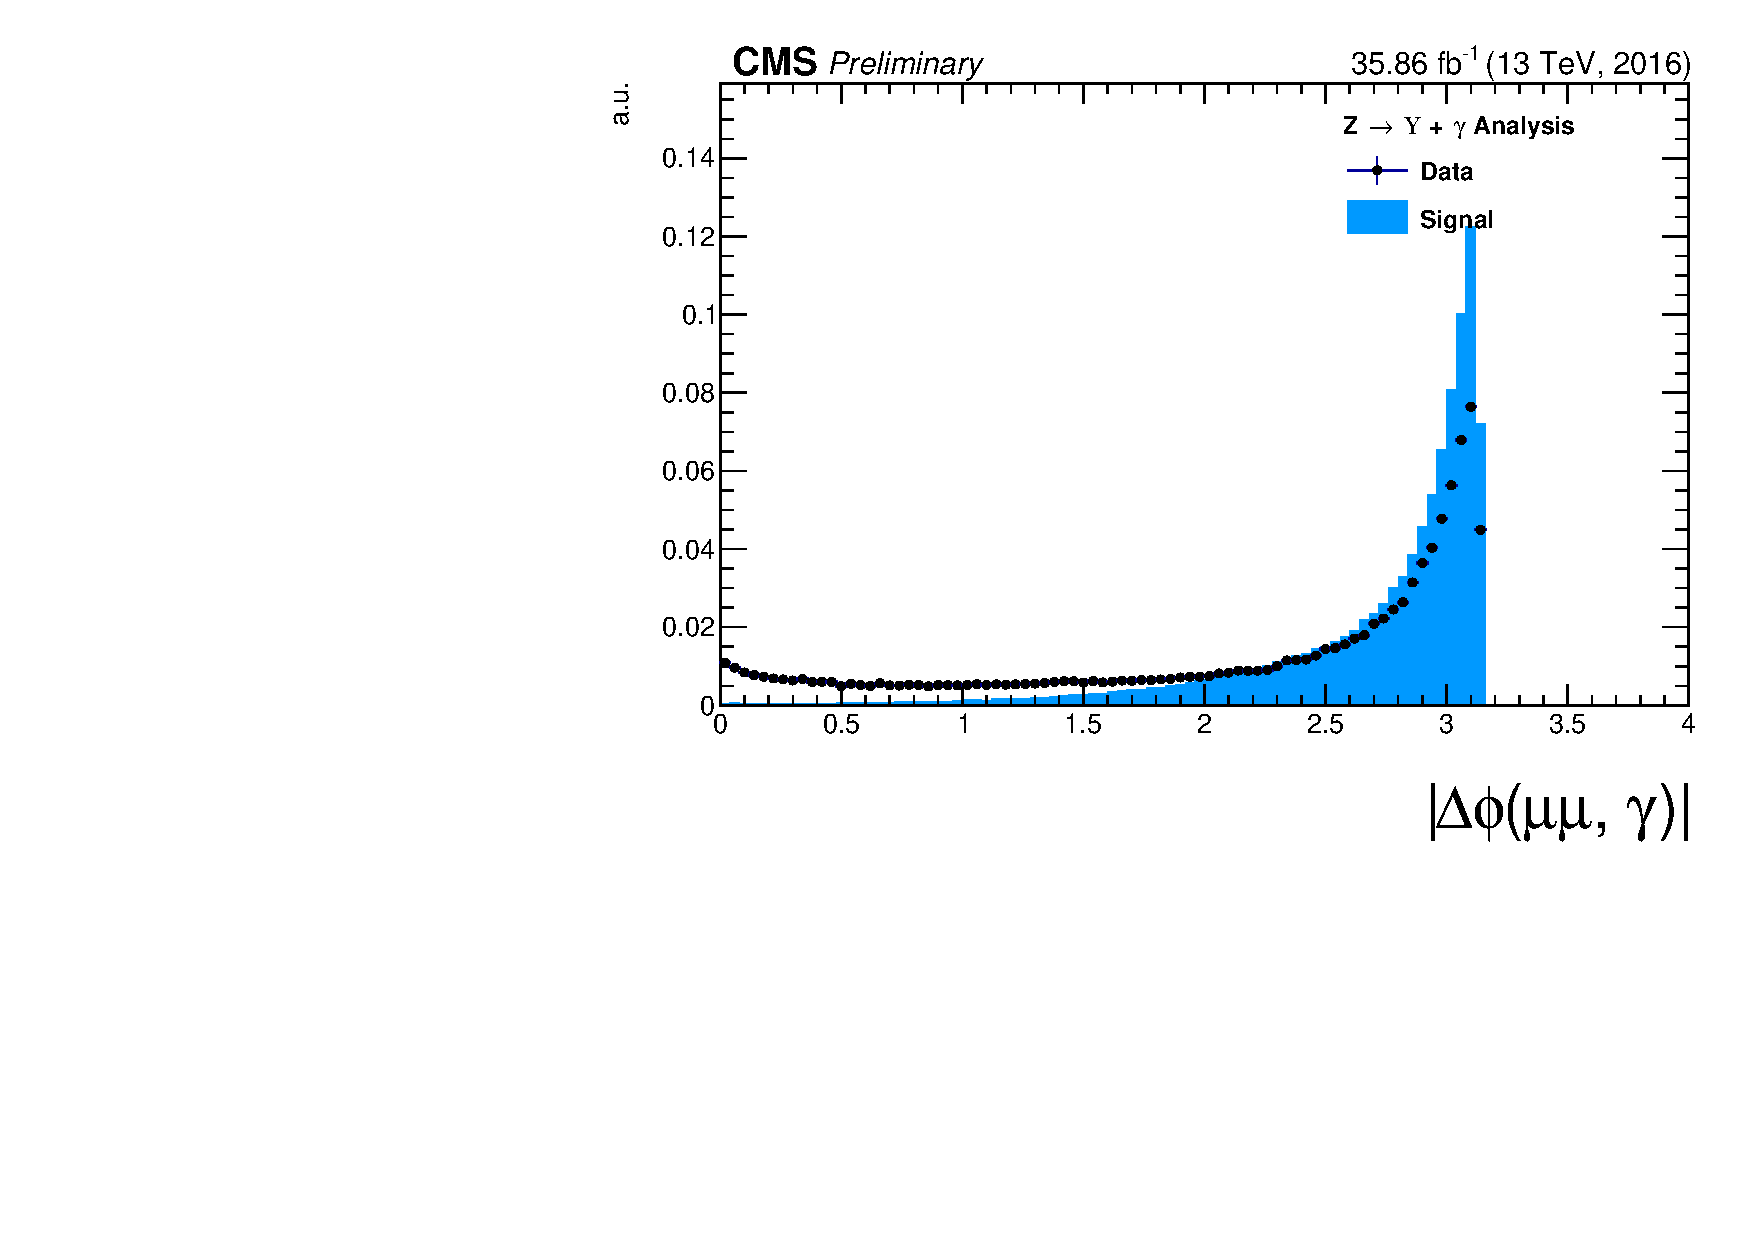
\includegraphics[width=0.45\textwidth]{figures_and_tables/outputPlots/ZtoUpsilon_Cat0_ZZZZZ/au/data_x_mc/noKinCuts/h_noKin_deltaPhi_Upsilon_Photon}\end{center}\vspace*{-.5cm}
\caption{Left: The $\Delta R$ distributions between reconstructed dimuon ($\mu\mu$) system and the photon. Right: absolute value of the $\Delta \phi$ between the dimuon system and the photon for Z decaying into $\Upsilon(1S,2S,3S)$ + $\gamma$ from data and signal events after Group I of selection cuts. The plots are normalized to the unit of area. The black dots are data collect by CMS while the blue distribution is related only to the signal Monte-Carlo generated samples.}
\label{fig:deltaRdeltaPhi_ZtoUpsilon_Cat0}
\end{figure}


%%%%%%% energy/mass ratio distributions for ZtoUpsilon_Cat0
\begin{figure}[!htbp]
\begin{center}
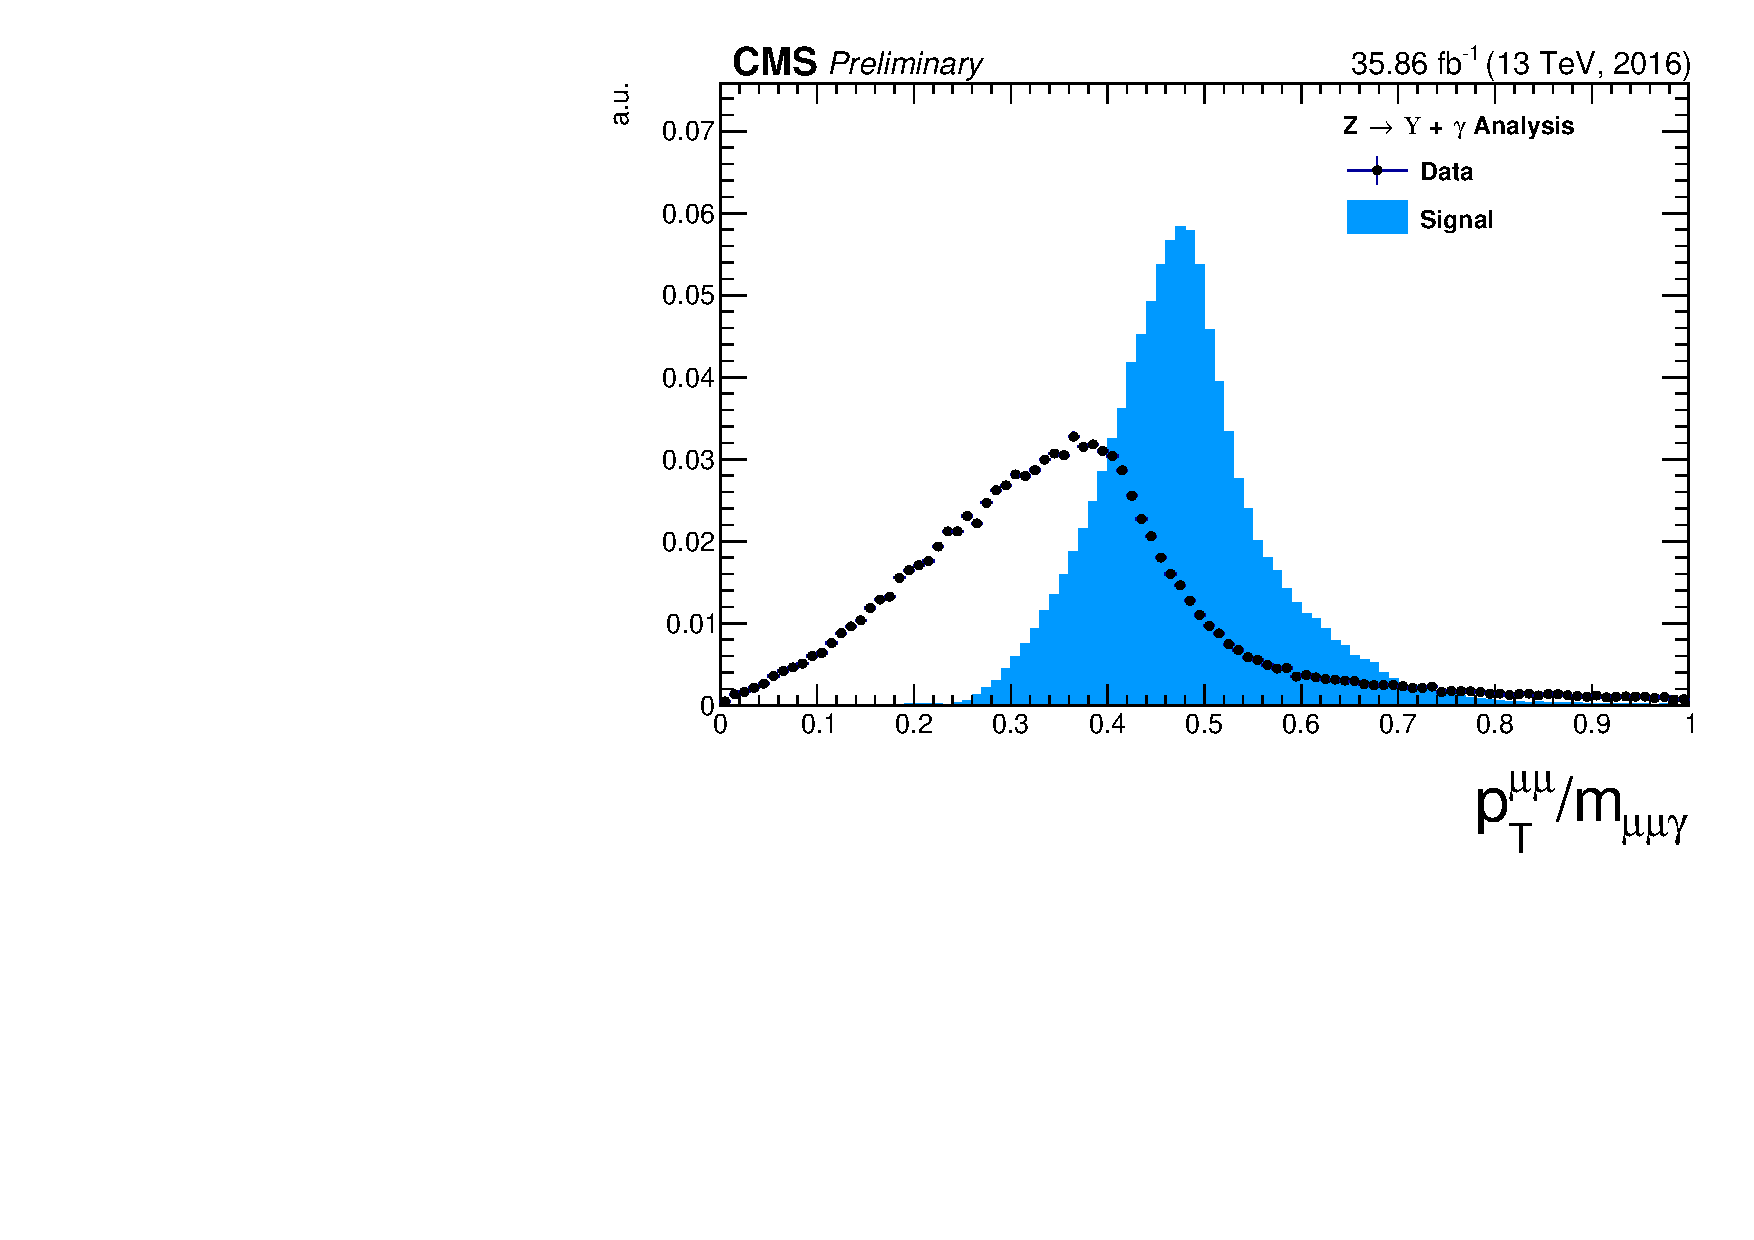
\includegraphics[width=0.45\textwidth]{figures_and_tables/outputPlots/ZtoUpsilon_Cat0_ZZZZZ/au/data_x_mc/noKinCuts/h_noKin_upsilonPt_over_zMass}\hspace*{1.cm}
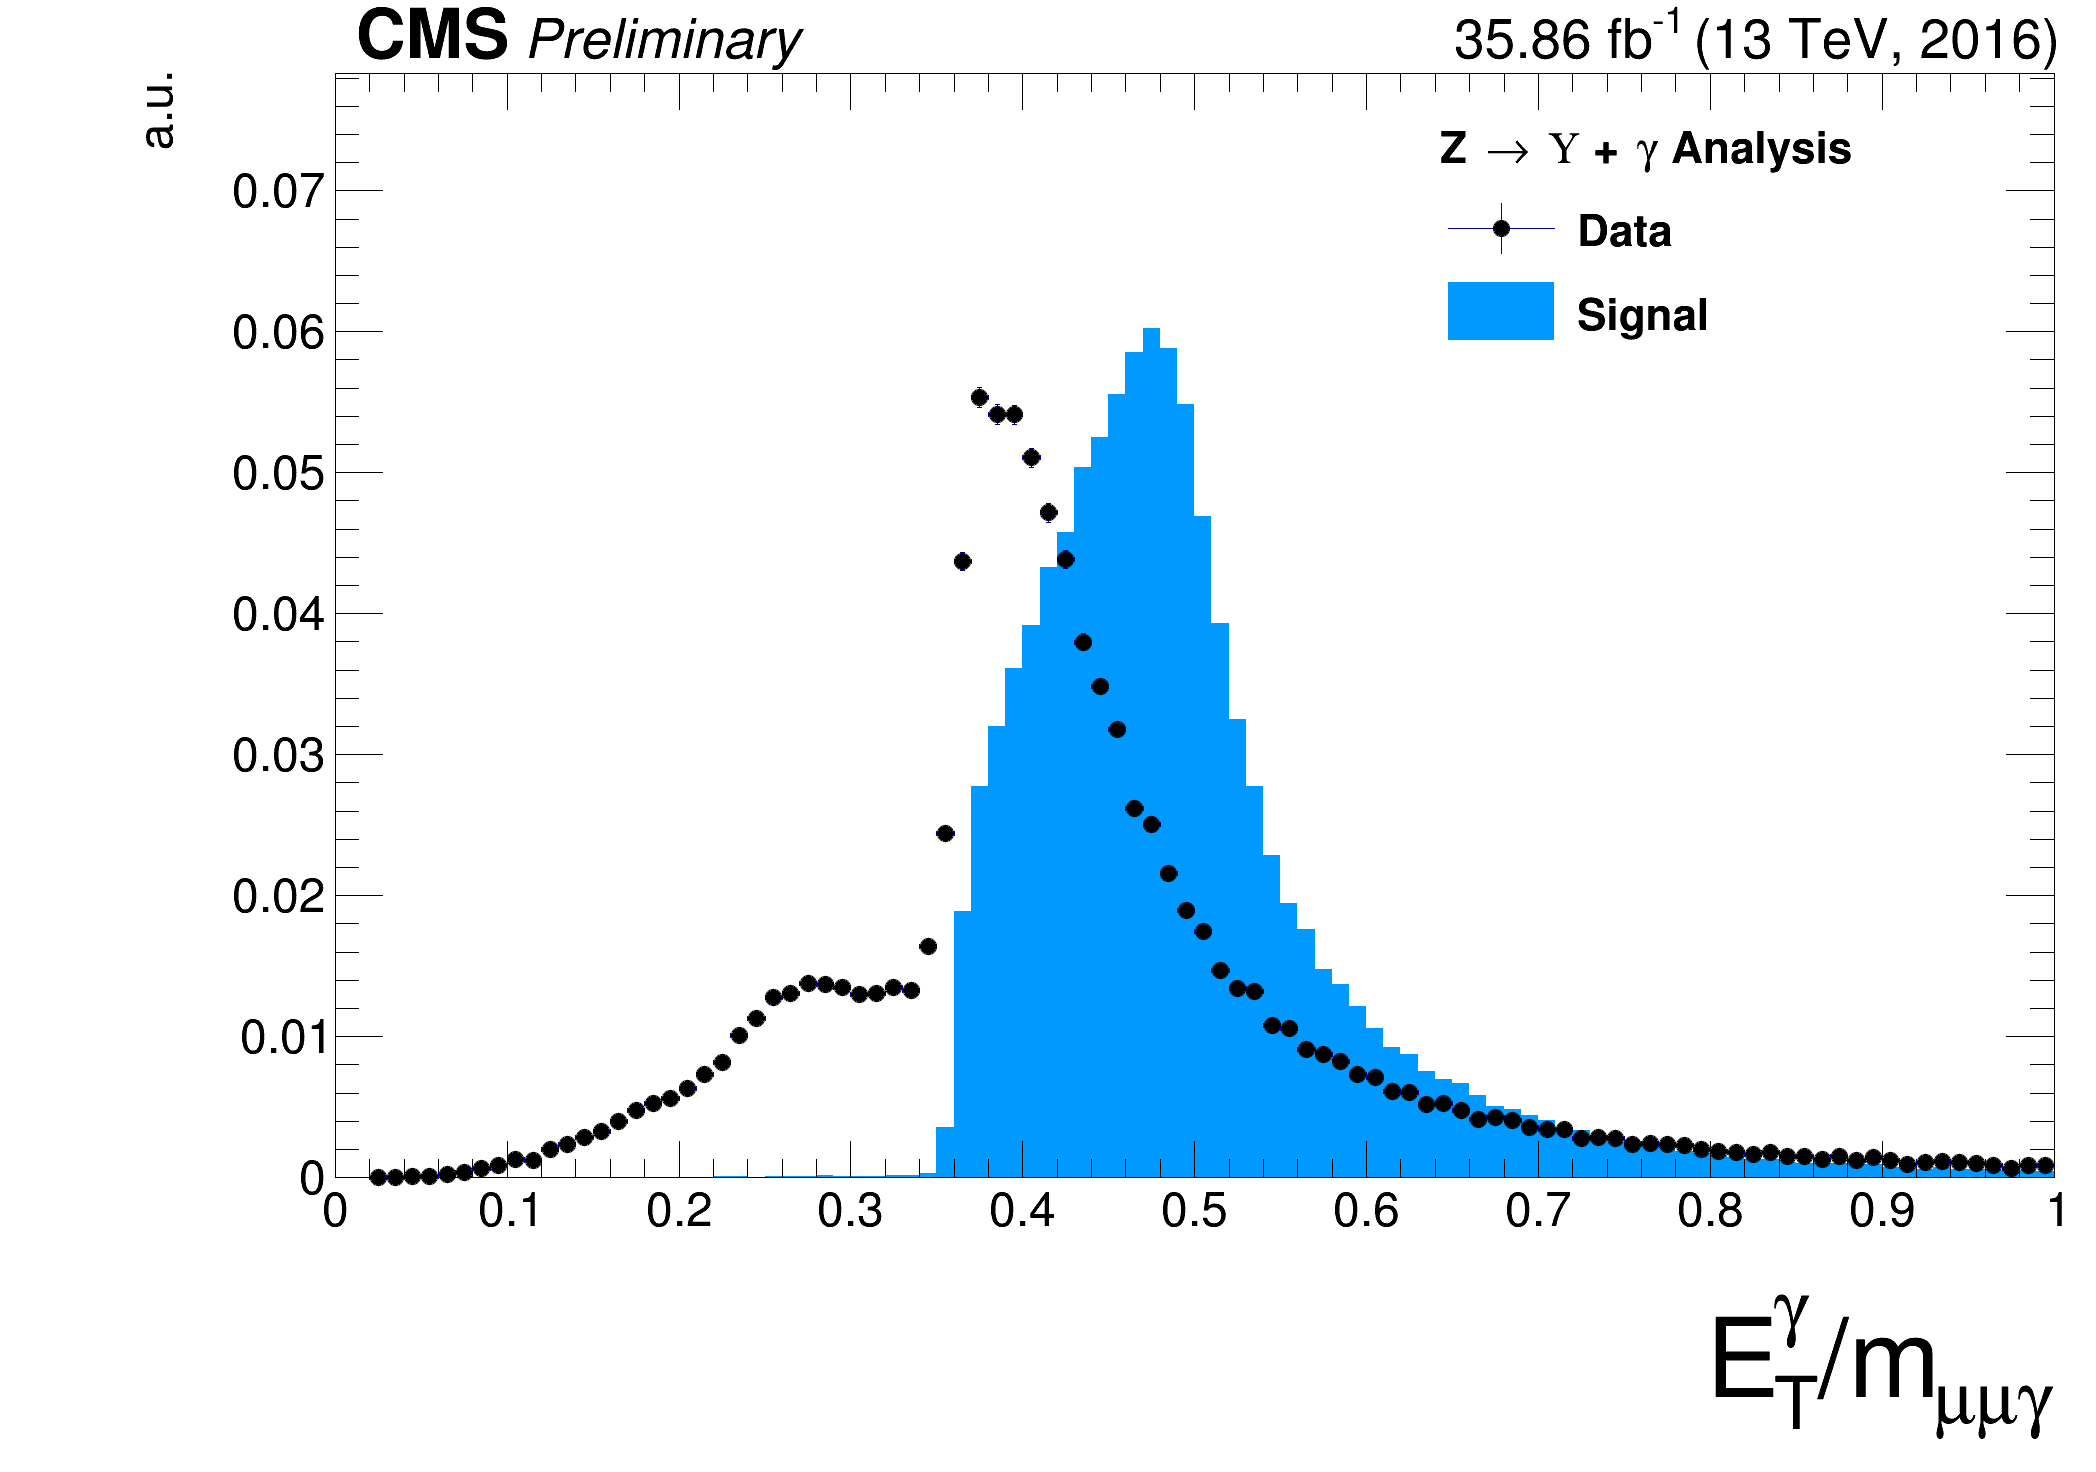
\includegraphics[width=0.45\textwidth]{figures_and_tables/outputPlots/ZtoUpsilon_Cat0_ZZZZZ/au/data_x_mc/noKinCuts/h_noKin_photonPt_over_zMass}
\end{center}\vspace*{-.5cm}
\caption{The ratio for the transverse momentum of the reconstructed Upsilon and the reconstructed Z mass ($p_{T}^{\mu\mu}/M_{\mu\mu\gamma}$ - left) and the ratio for the transverse energy of the reconstructed Photon and the reconstructed Z mass ($E_{T}^{\gamma}/M_{\mu\mu\gamma}$ - right) distribution for Z decaying into $\Upsilon(1S,2S,3S)$ + $\gamma$ from data and signal events after Group I of selection cuts. The plots are normalized to the unit of area. The black dots are data collect by CMS while the blue distribution is related only to the signal Monte-Carlo generated samples.}
\label{fig:energy_ration_ZtoUpsilon_Cat0}
\end{figure}

%%%%%%%%% dimuon mass distributions for ZtoUpsilon_Cat0
\begin{figure}[!htbp]
\begin{center}
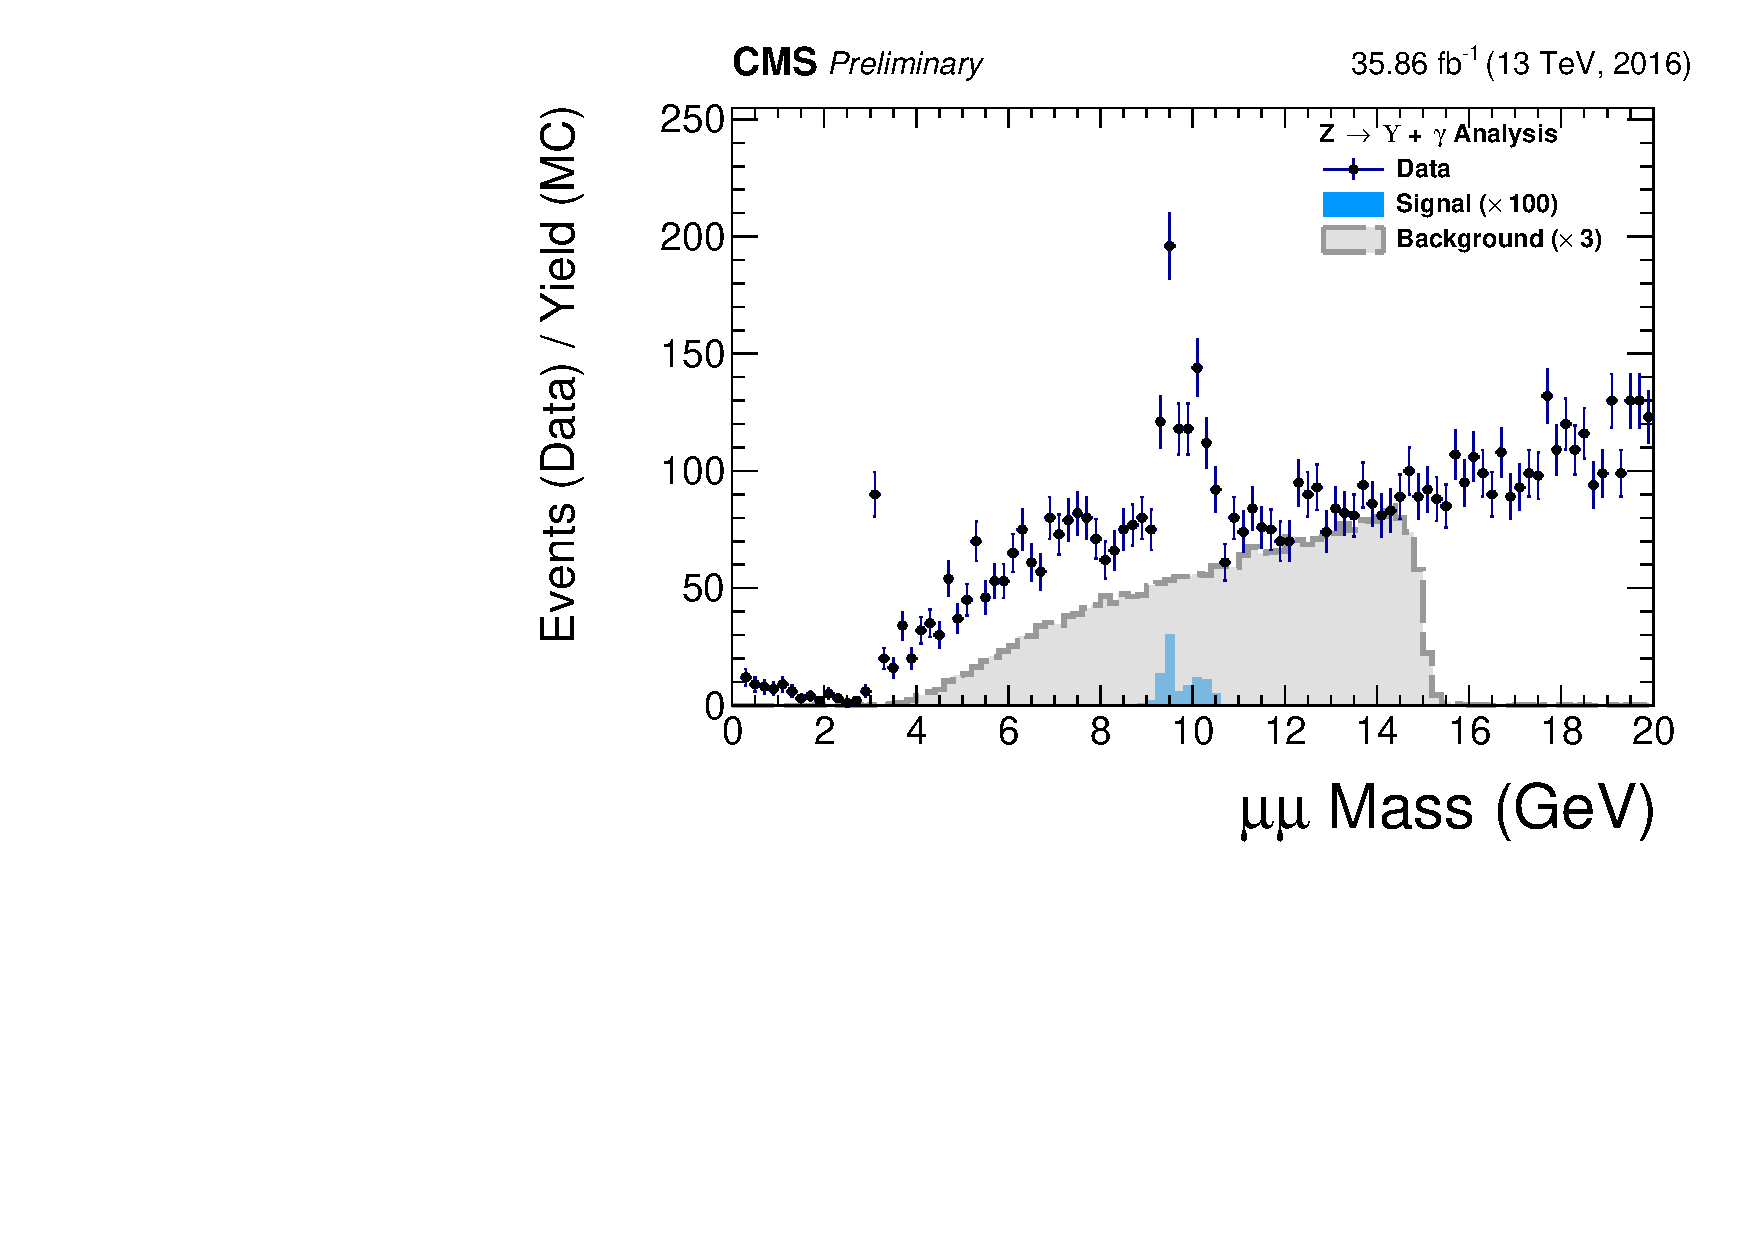
\includegraphics[width=0.45\textwidth]{figures_and_tables/outputPlots/ZtoUpsilon_Cat0_ZZZZZ/nEvts/data_x_mc/noKinCuts/h_noKin_Upsilon_Mass_Signal_and_Background_LargeRange}\hspace*{1.cm}
\end{center}\vspace*{-.5cm}
\caption{The dimuon mass distribution of the reconstructed $\Upsilon (1S,2S,3S)$ from data and signal events for Z decaying after Group I of selection cuts. The plot is normalized to the number of events. "Signal" stands for the $Z \rightarrow \Upsilon (1S,2S,3S) + \gamma$ sample (scaled by a factor of $\times 100$) and "Background" corresponds to the resonant background ($Z \rightarrow \mu\mu\gamma_{FSR}$) sample (scaled by a factor of x3).}
\label{fig:dimuon_mass_ZtoUpsilon_Cat0}
\end{figure}

%%%%%%%%%%%%


%CONTROL PLOTS
%%$\pT$ muon distributions for HtoUpsilon_Cat0
\begin{figure}[!htbp]
\begin{center}
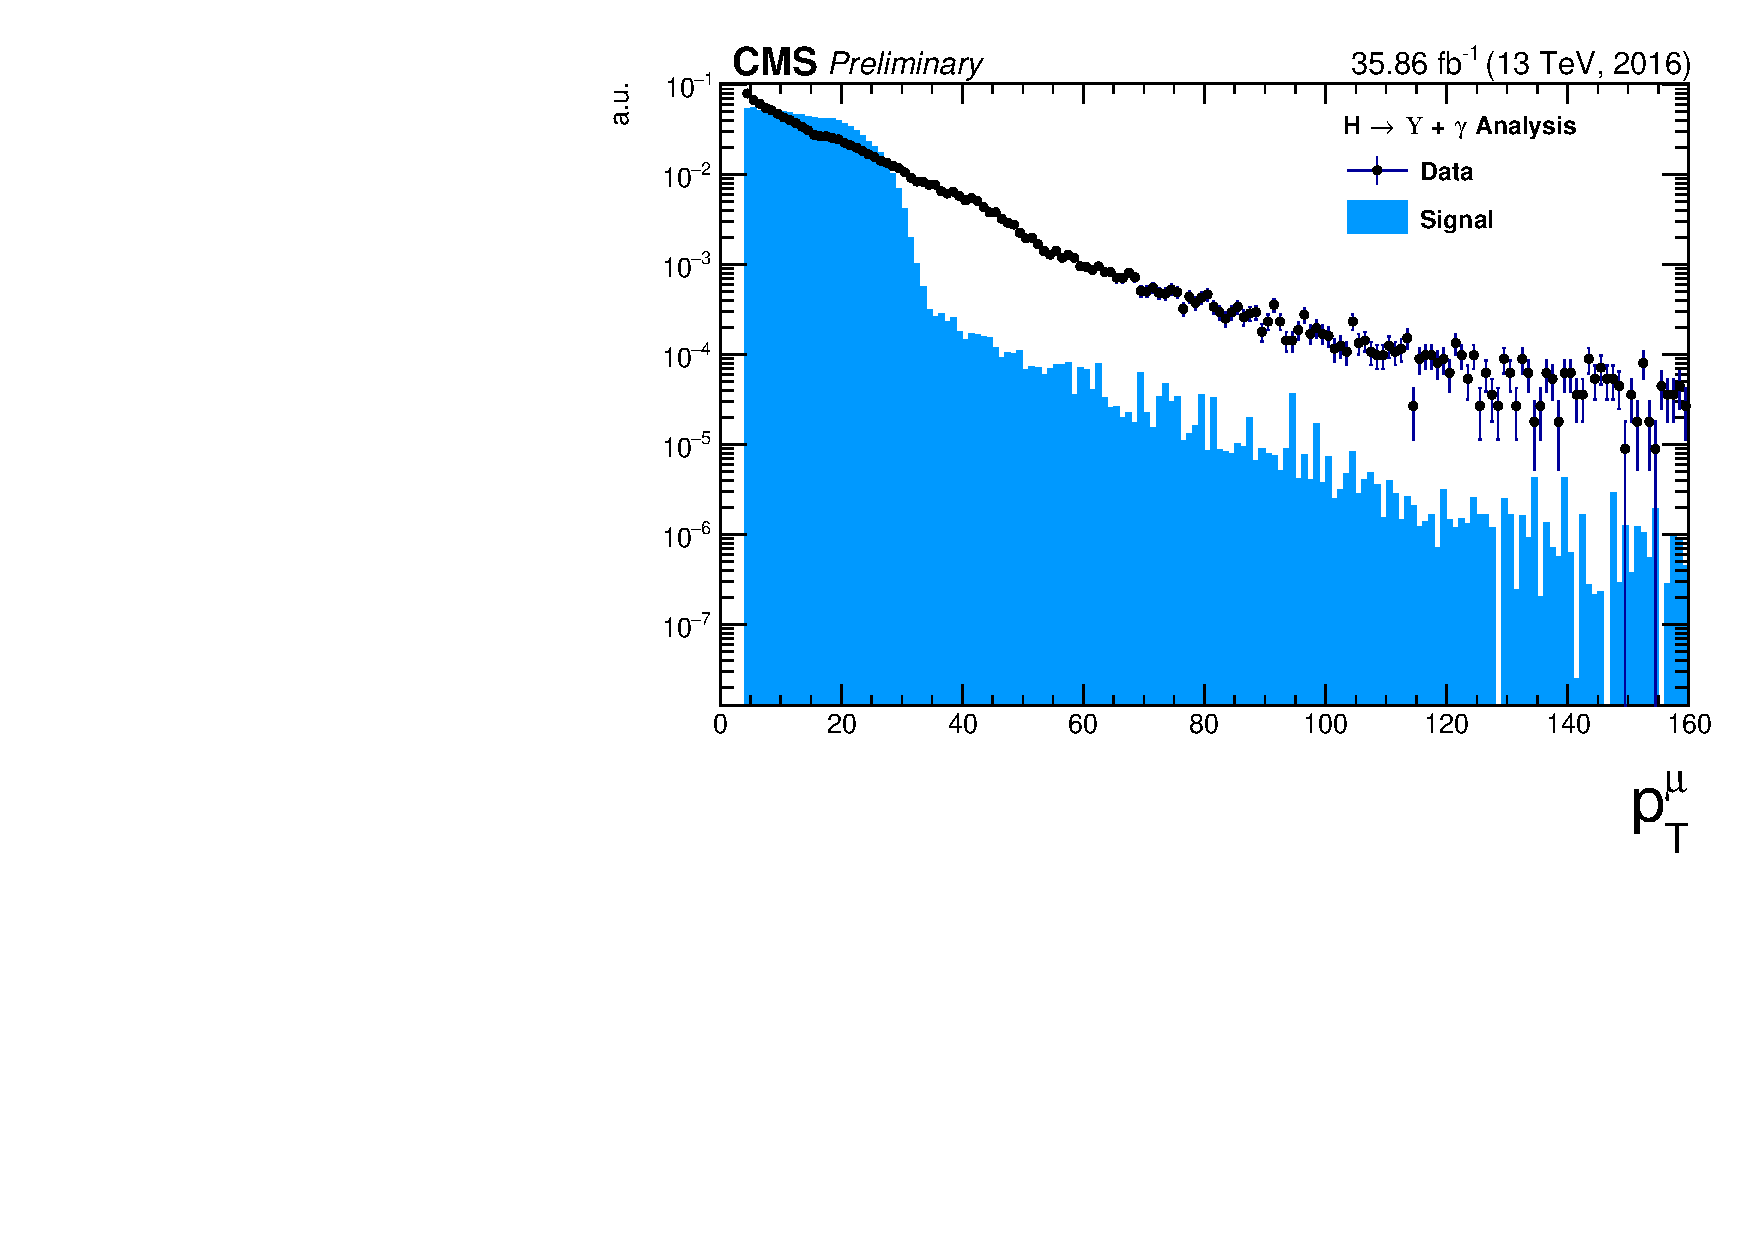
\includegraphics[width=0.45\textwidth]{figures_and_tables/outputPlots/HtoUpsilon_Cat0_ZZZZZ/au/data_x_mc/noKinCuts/h_noKin_TrailingMu_pt}\hspace*{1.cm}
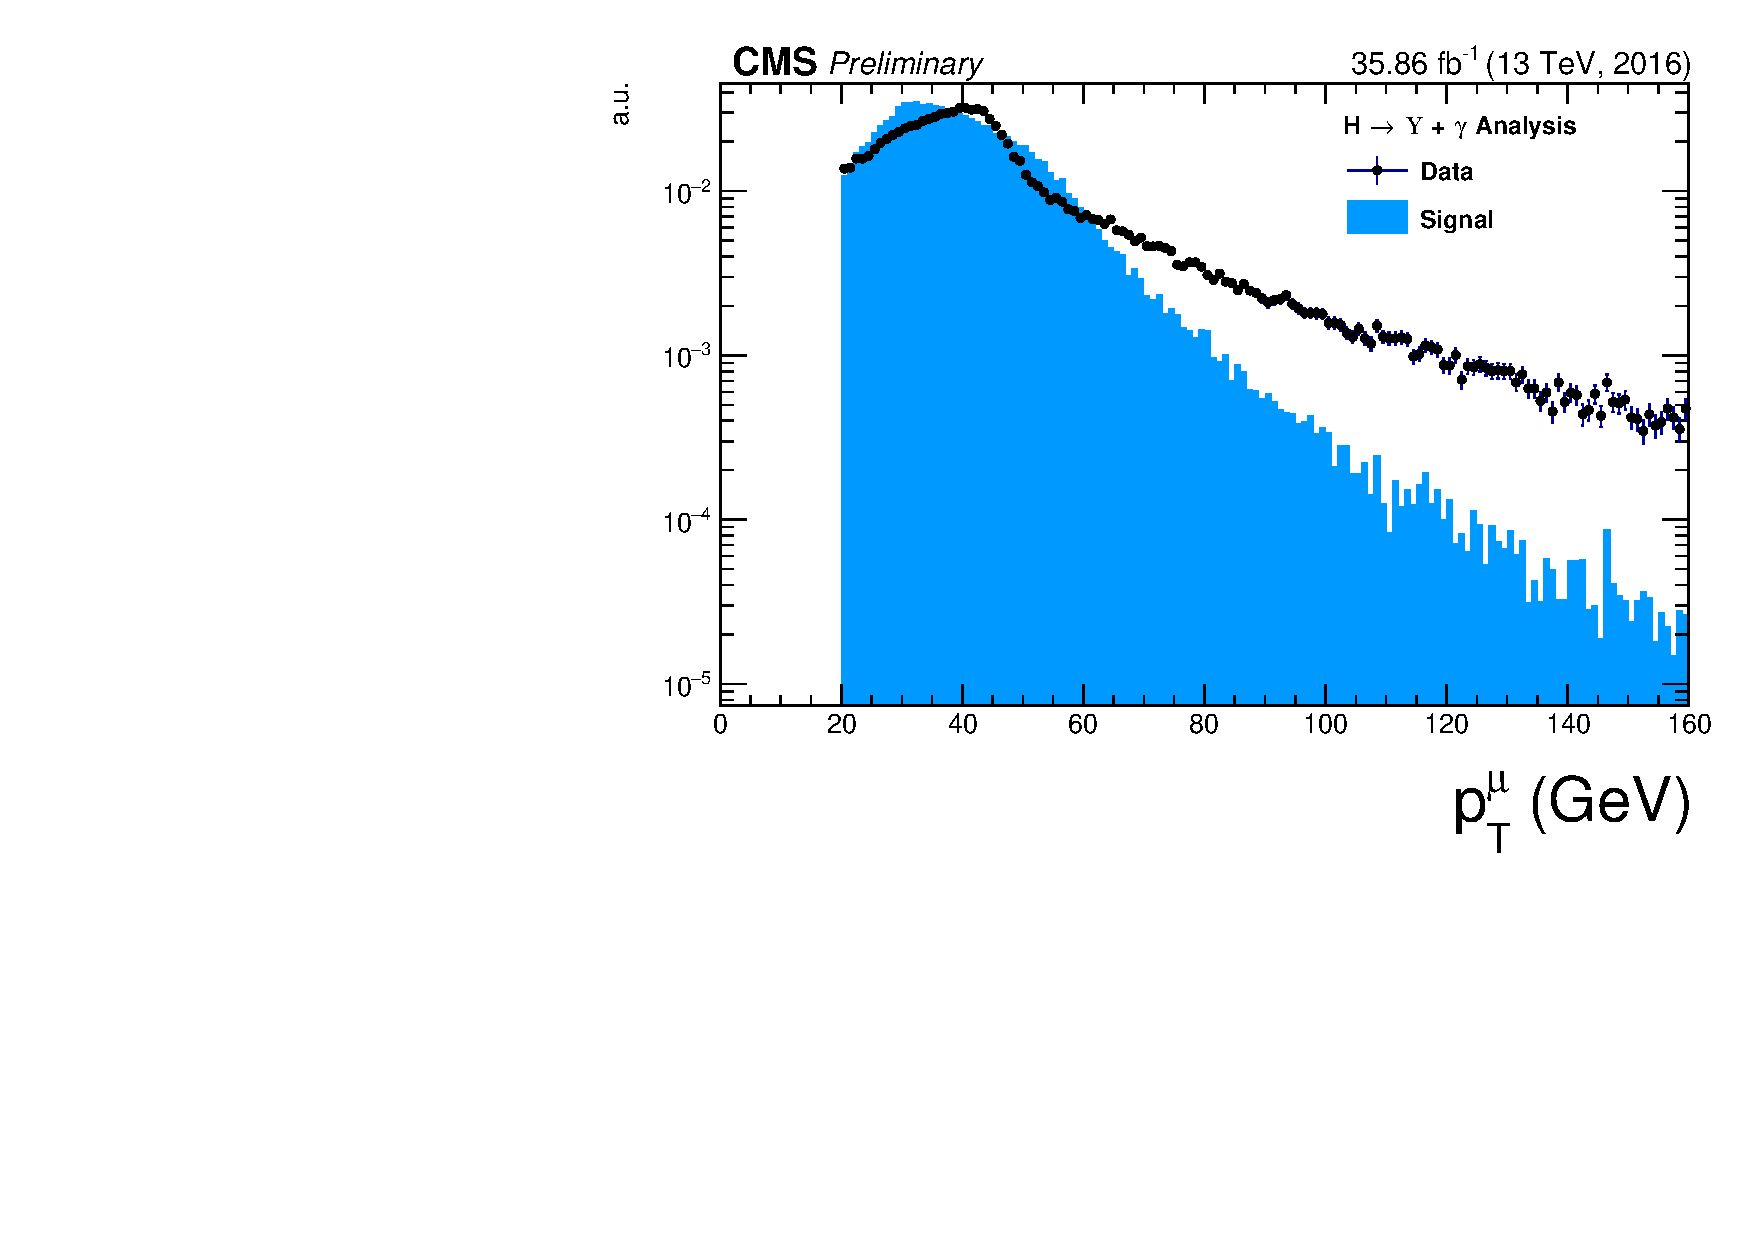
\includegraphics[width=0.45\textwidth]{figures_and_tables/outputPlots/HtoUpsilon_Cat0_ZZZZZ/au/data_x_mc/noKinCuts/h_noKin_LeadingMu_pt}
\end{center}\vspace*{-.5cm}
\caption{The \PT muon distributions from data and signal events for Higgs decaying into $\Upsilon(1S,2S,3S)$ + $\gamma$ after Group I of selection cuts, where on left are presenting the trailing muons and on right are the leading muons. The plots are normalized to the unit of area. The black dots are data collect by CMS while the blue distribution is related only to the signal Monte-Carlo generated samples.}
\label{fig:pTMuons_HtoUpsilon_Cat0}
\end{figure}


%%%%%%%$\eta$ muon distributions for HtoUpsilon_Cat0
\begin{figure}[!htbp]
\begin{center}
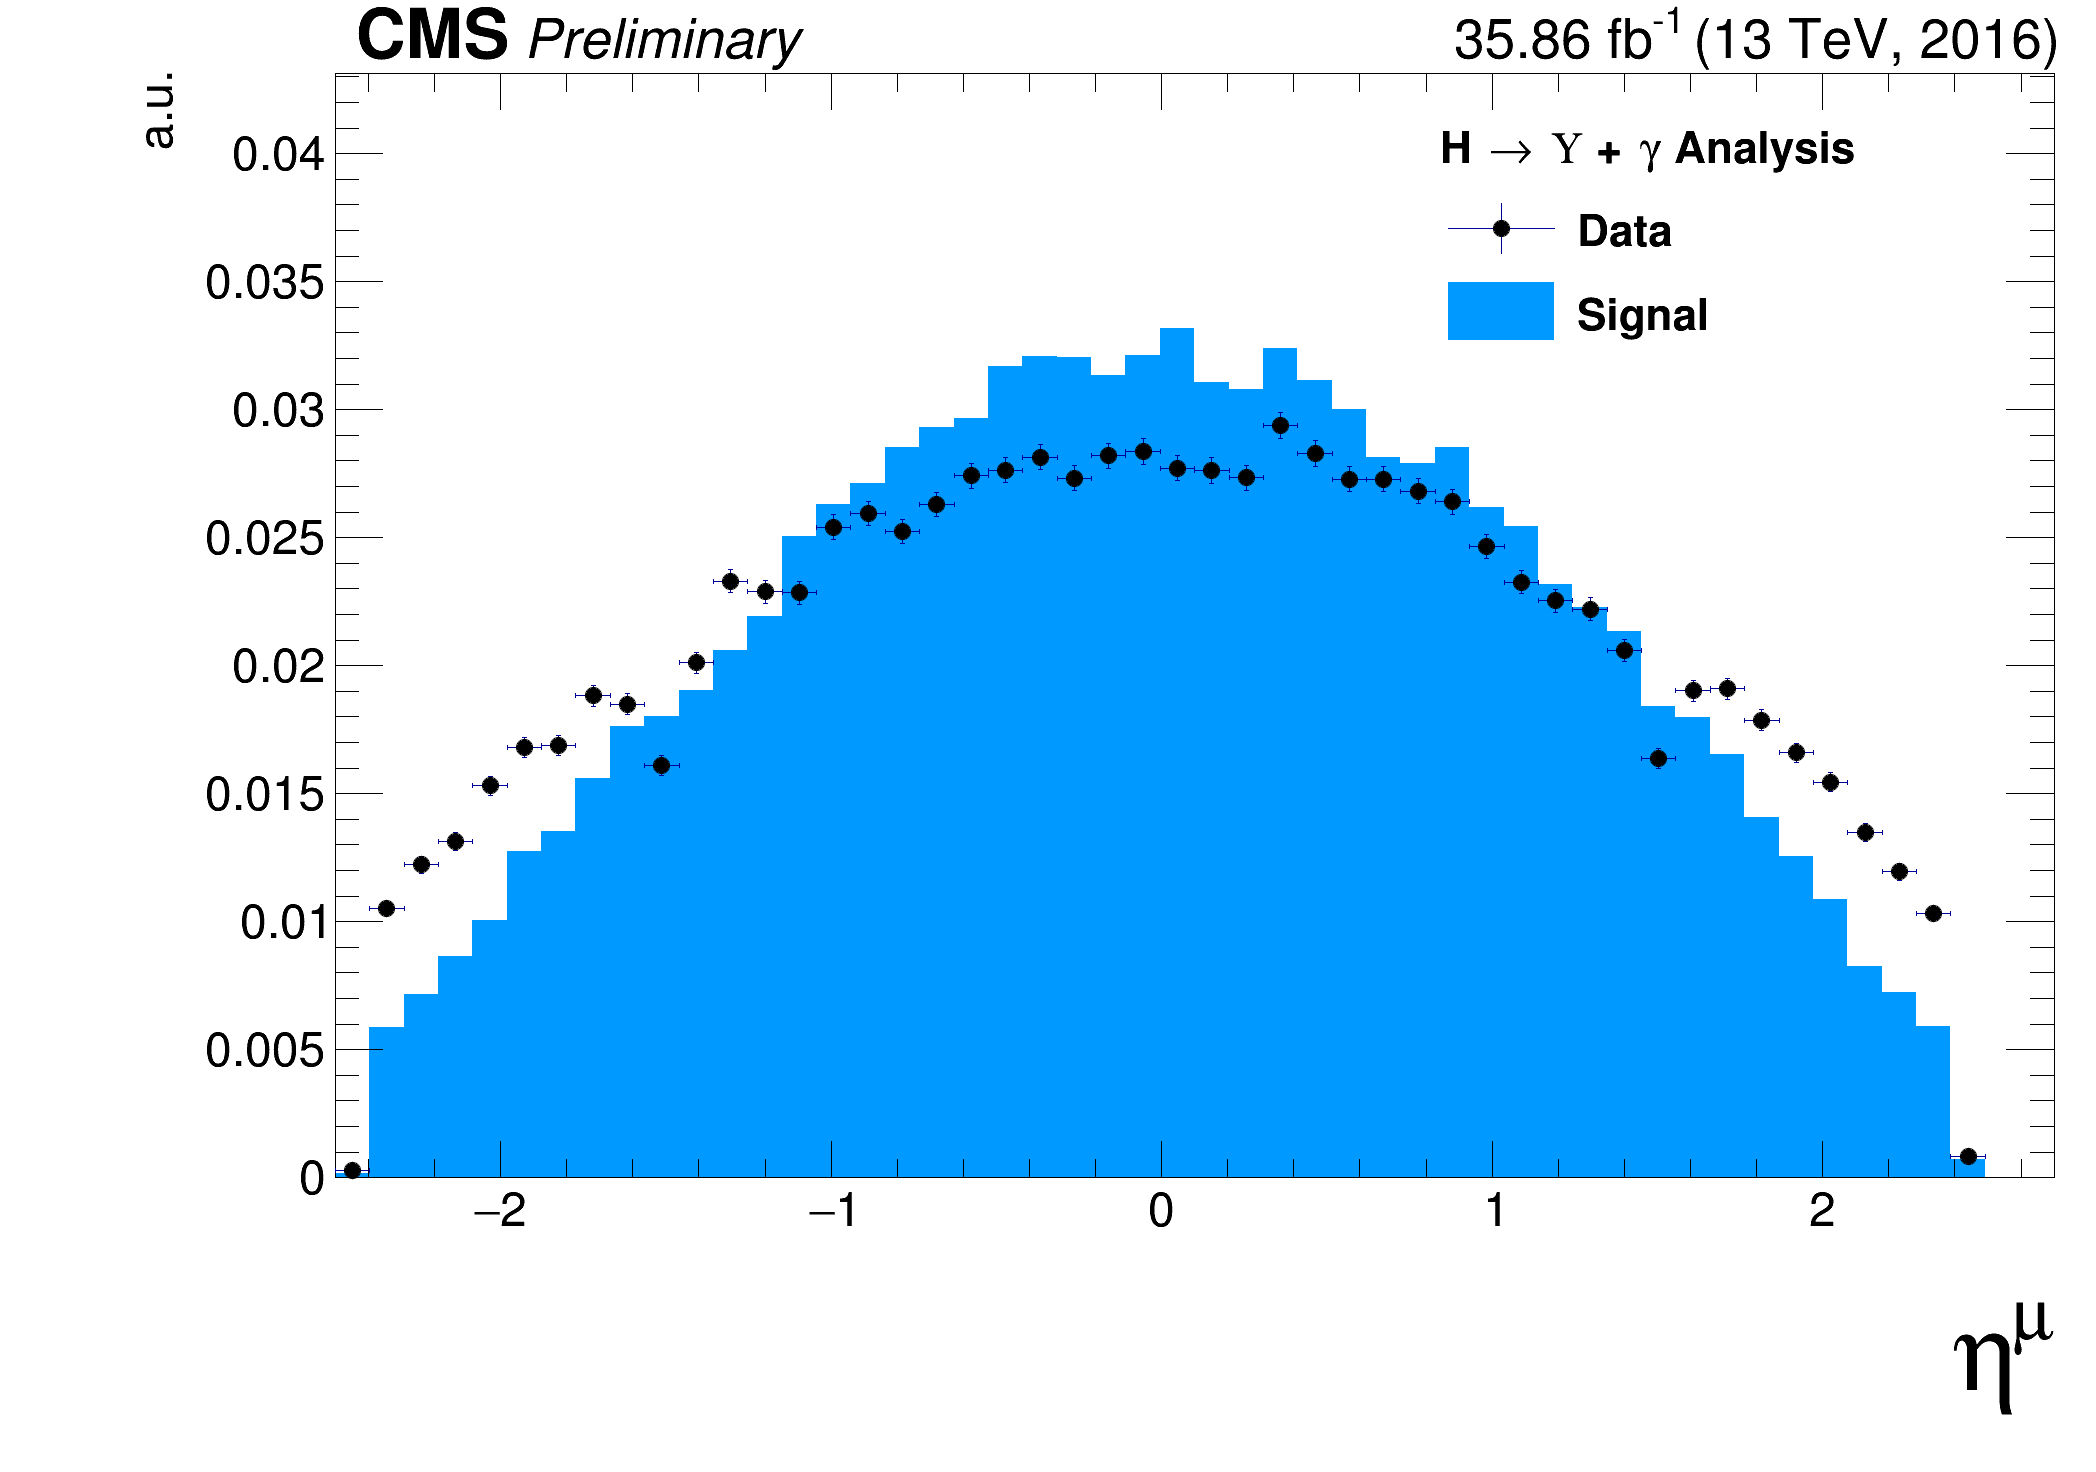
\includegraphics[width=0.45\textwidth]{figures_and_tables/outputPlots/HtoUpsilon_Cat0_ZZZZZ/au/data_x_mc/noKinCuts/h_noKin_TrailingMu_eta}\hspace*{1.cm}
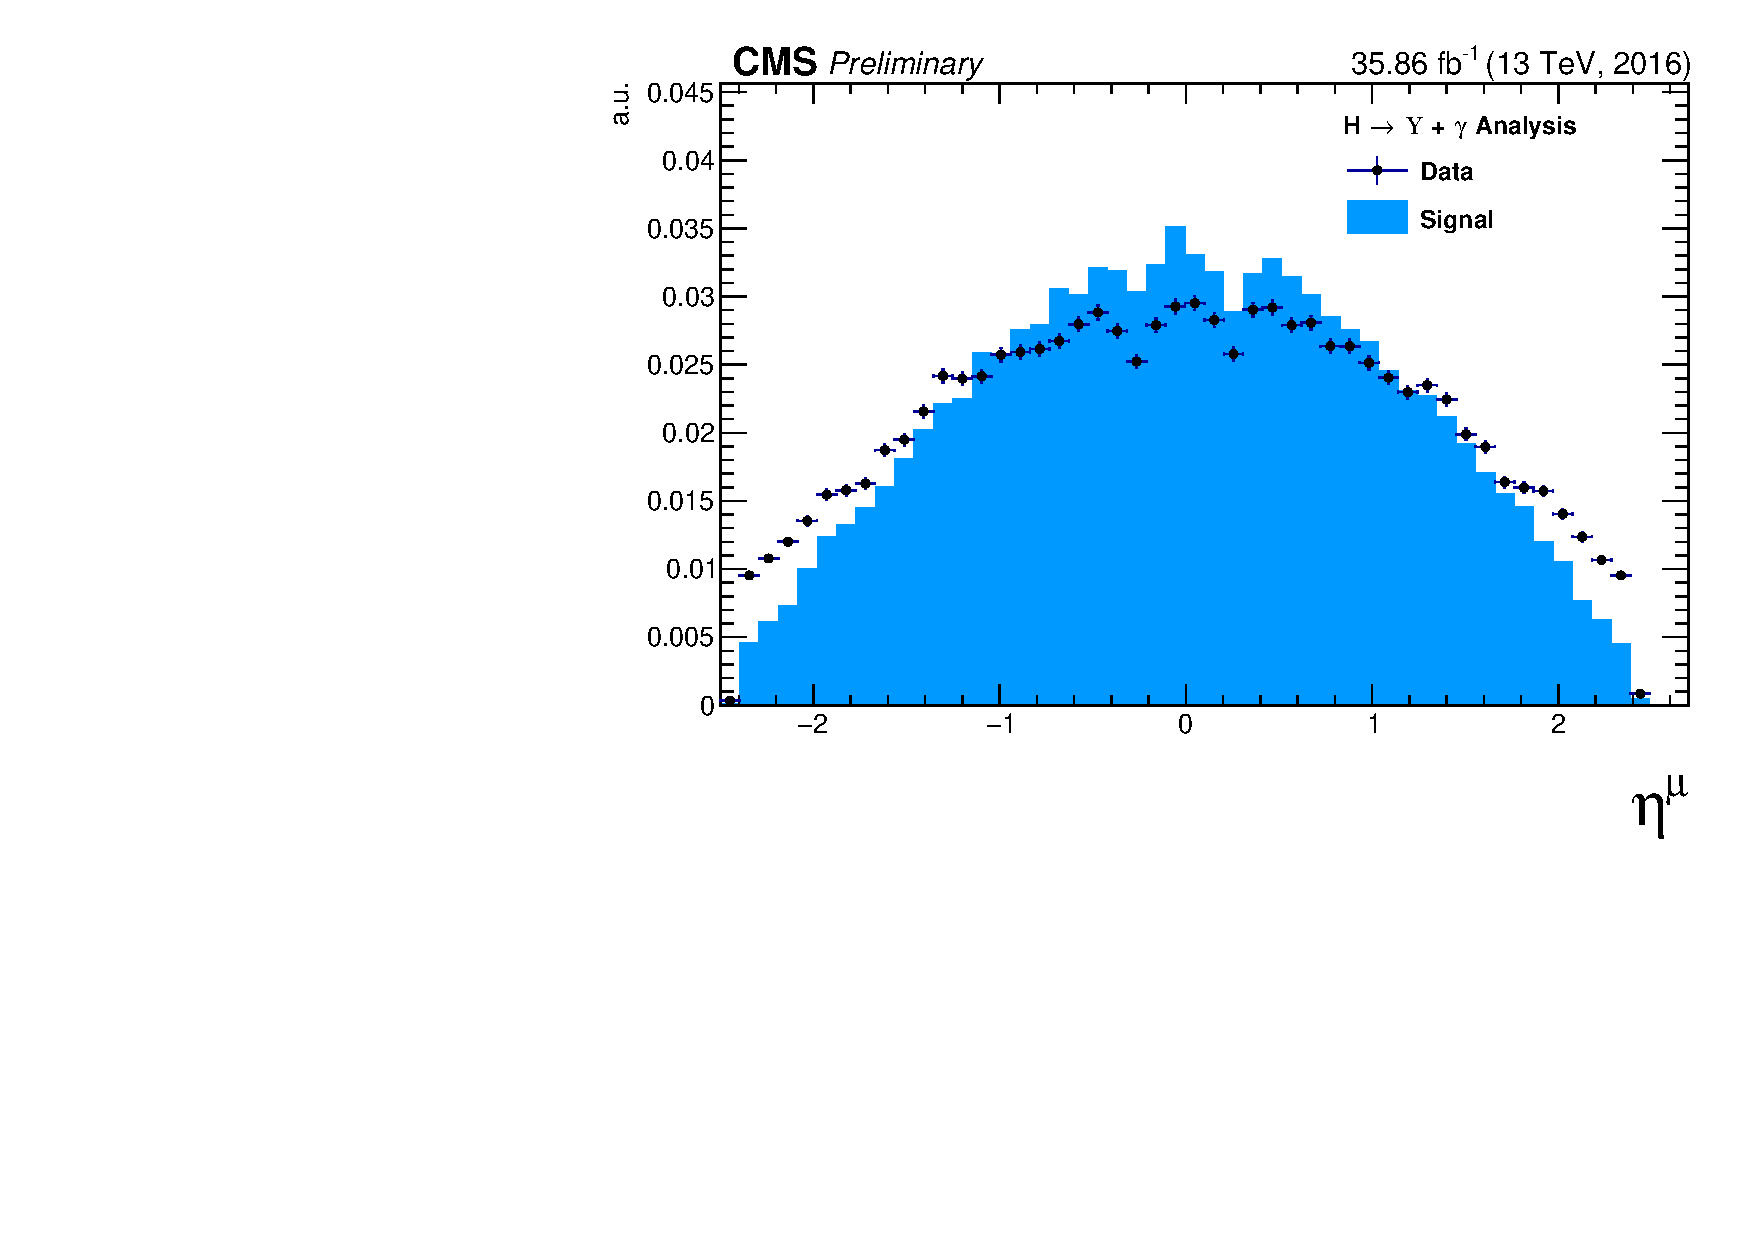
\includegraphics[width=0.45\textwidth]{figures_and_tables/outputPlots/HtoUpsilon_Cat0_ZZZZZ/au/data_x_mc/noKinCuts/h_noKin_LeadingMu_eta}
\end{center}\vspace*{-.5cm}
\caption{The $\eta$ muon distributions from data and signal events of Higgs decaying into $\Upsilon(1S,2S,3S)$ + $\gamma$ after Group I of selection cuts, where on left are presenting the trailing muons and on right are the leading muons. The plots are normalized to the unit of area. The black dots are data collect by CMS while the blue distribution is related only to the signal Monte-Carlo generated samples.}
\label{fig:etaMuons_HtoUpsilon_Cat0}
\end{figure}

%%%%%%%%% $\phi$ muon distributions for HtoUpsilon_Cat0
\begin{figure}[!htbp]
\begin{center}
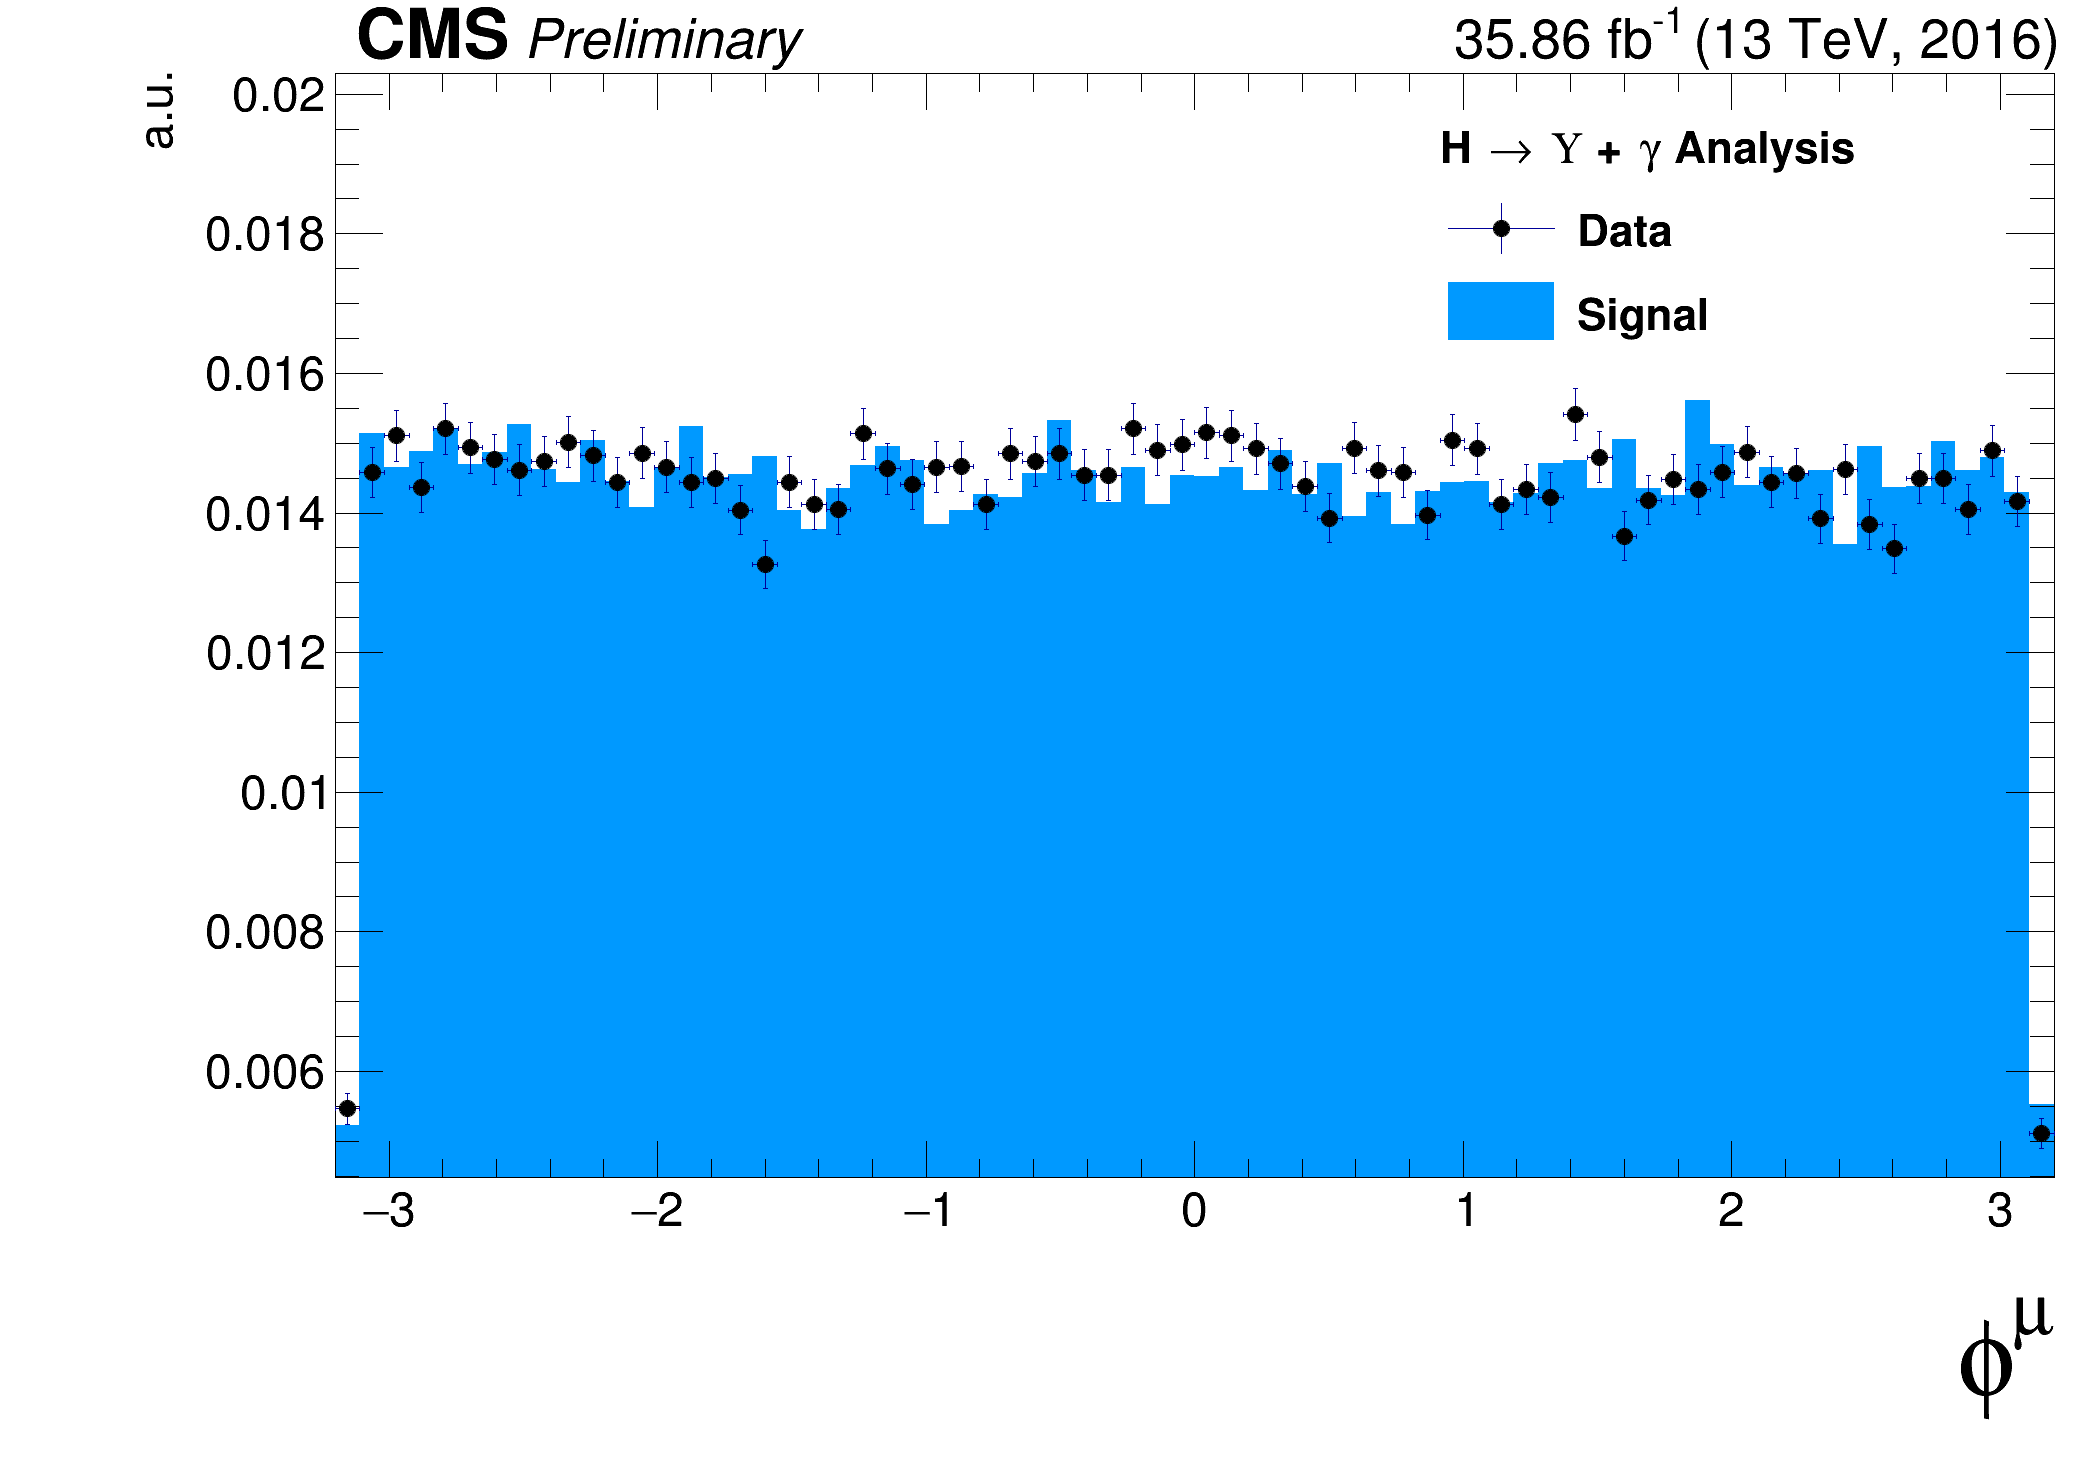
\includegraphics[width=0.45\textwidth]{figures_and_tables/outputPlots/HtoUpsilon_Cat0_ZZZZZ/au/data_x_mc/noKinCuts/h_noKin_TrailingMu_phi}\hspace*{1.cm}
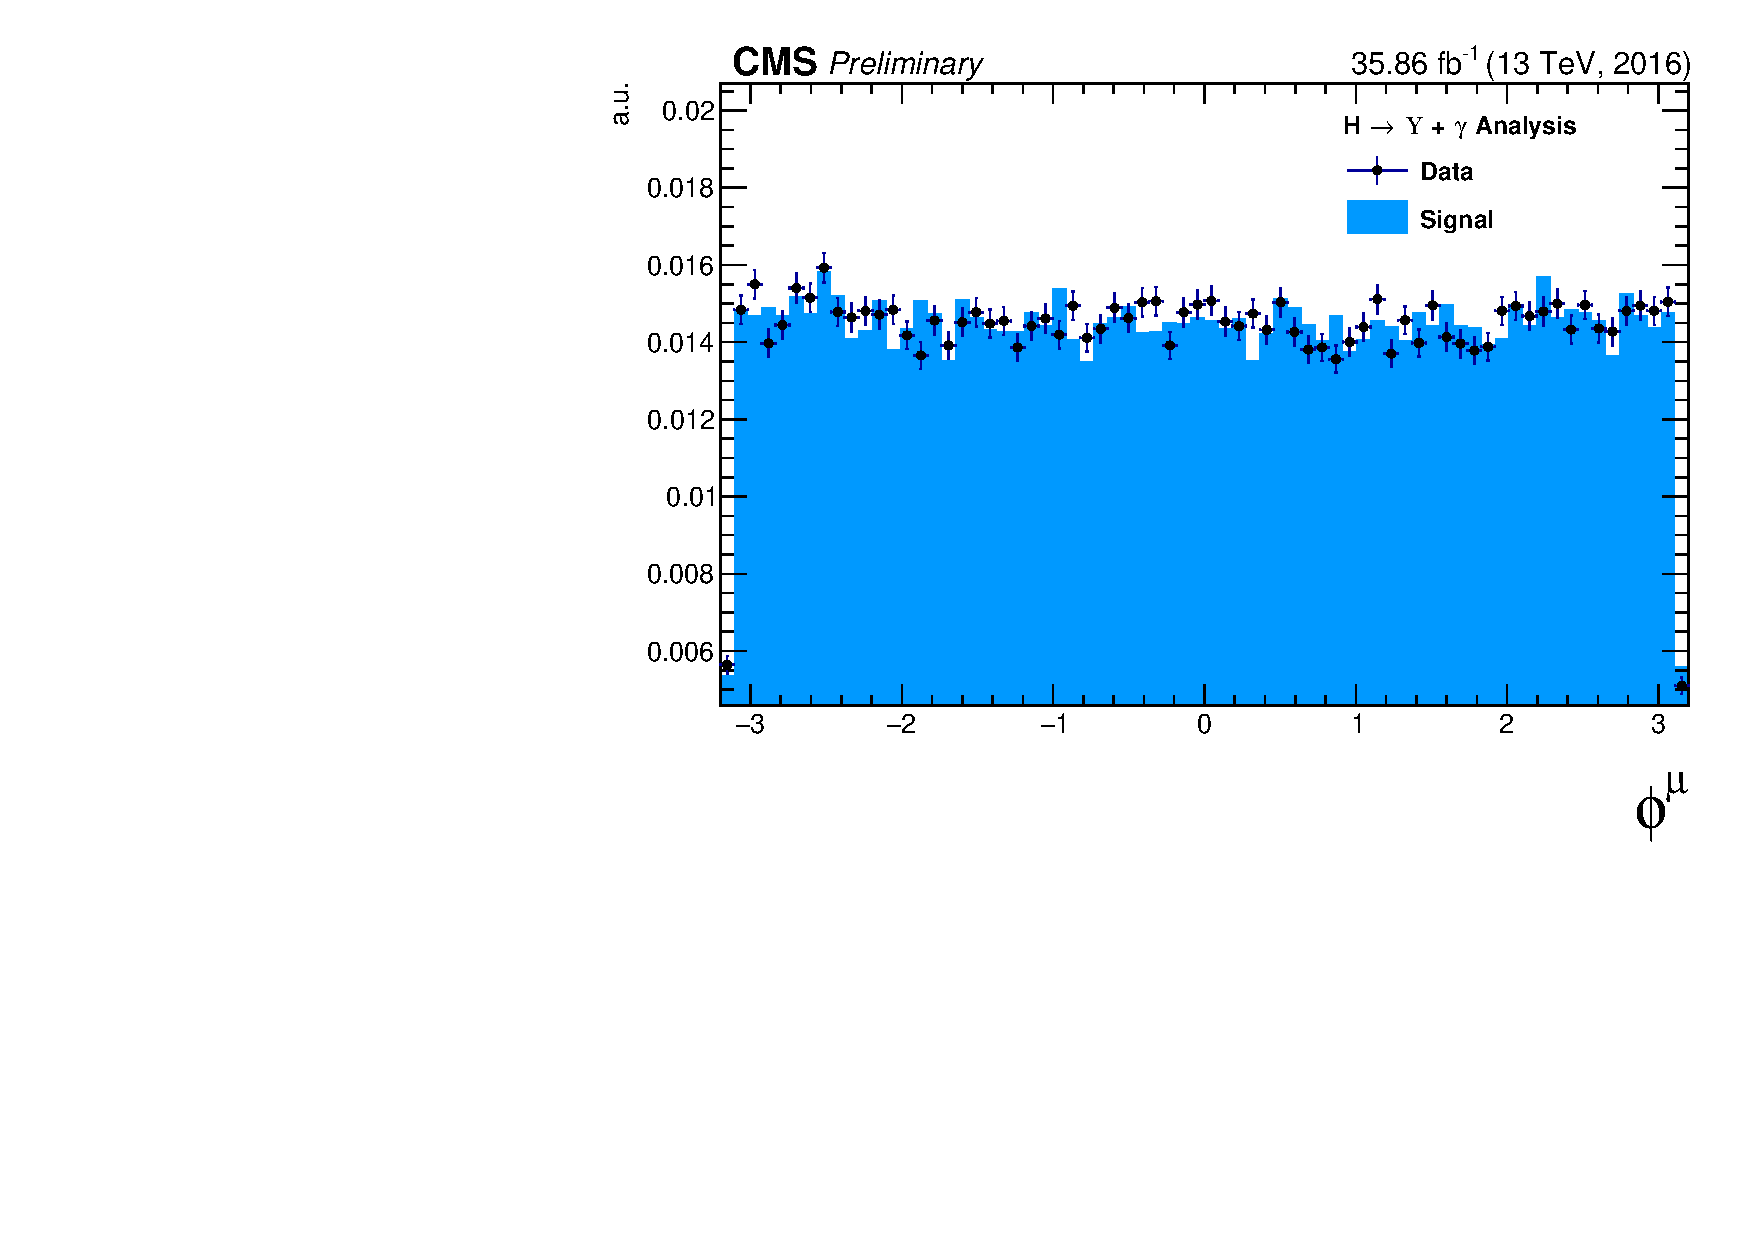
\includegraphics[width=0.45\textwidth]{figures_and_tables/outputPlots/HtoUpsilon_Cat0_ZZZZZ/au/data_x_mc/noKinCuts/h_noKin_LeadingMu_phi}
\end{center}\vspace*{-.5cm}
\caption{The $\phi$ muon distributions from data and signal events of Higgs decaying into $\Upsilon(1S,2S,3S)$ + $\gamma$ after Group I of selection cuts, where on left are presenting the trailing muons and on right are the leading muons. The plots are normalized to the unit of area. The black dots are data collect by CMS while the blue distribution is related only to the signal Monte-Carlo generated samples.}
\label{fig:phiMuons_HtoUpsilon_Cat0}
\end{figure}

%%%%%%%%%%%%%

%photon
%%$\pT$ Photon distributions for HtoUpsilon_Cat0
\begin{figure}[!htbp]
\begin{center}
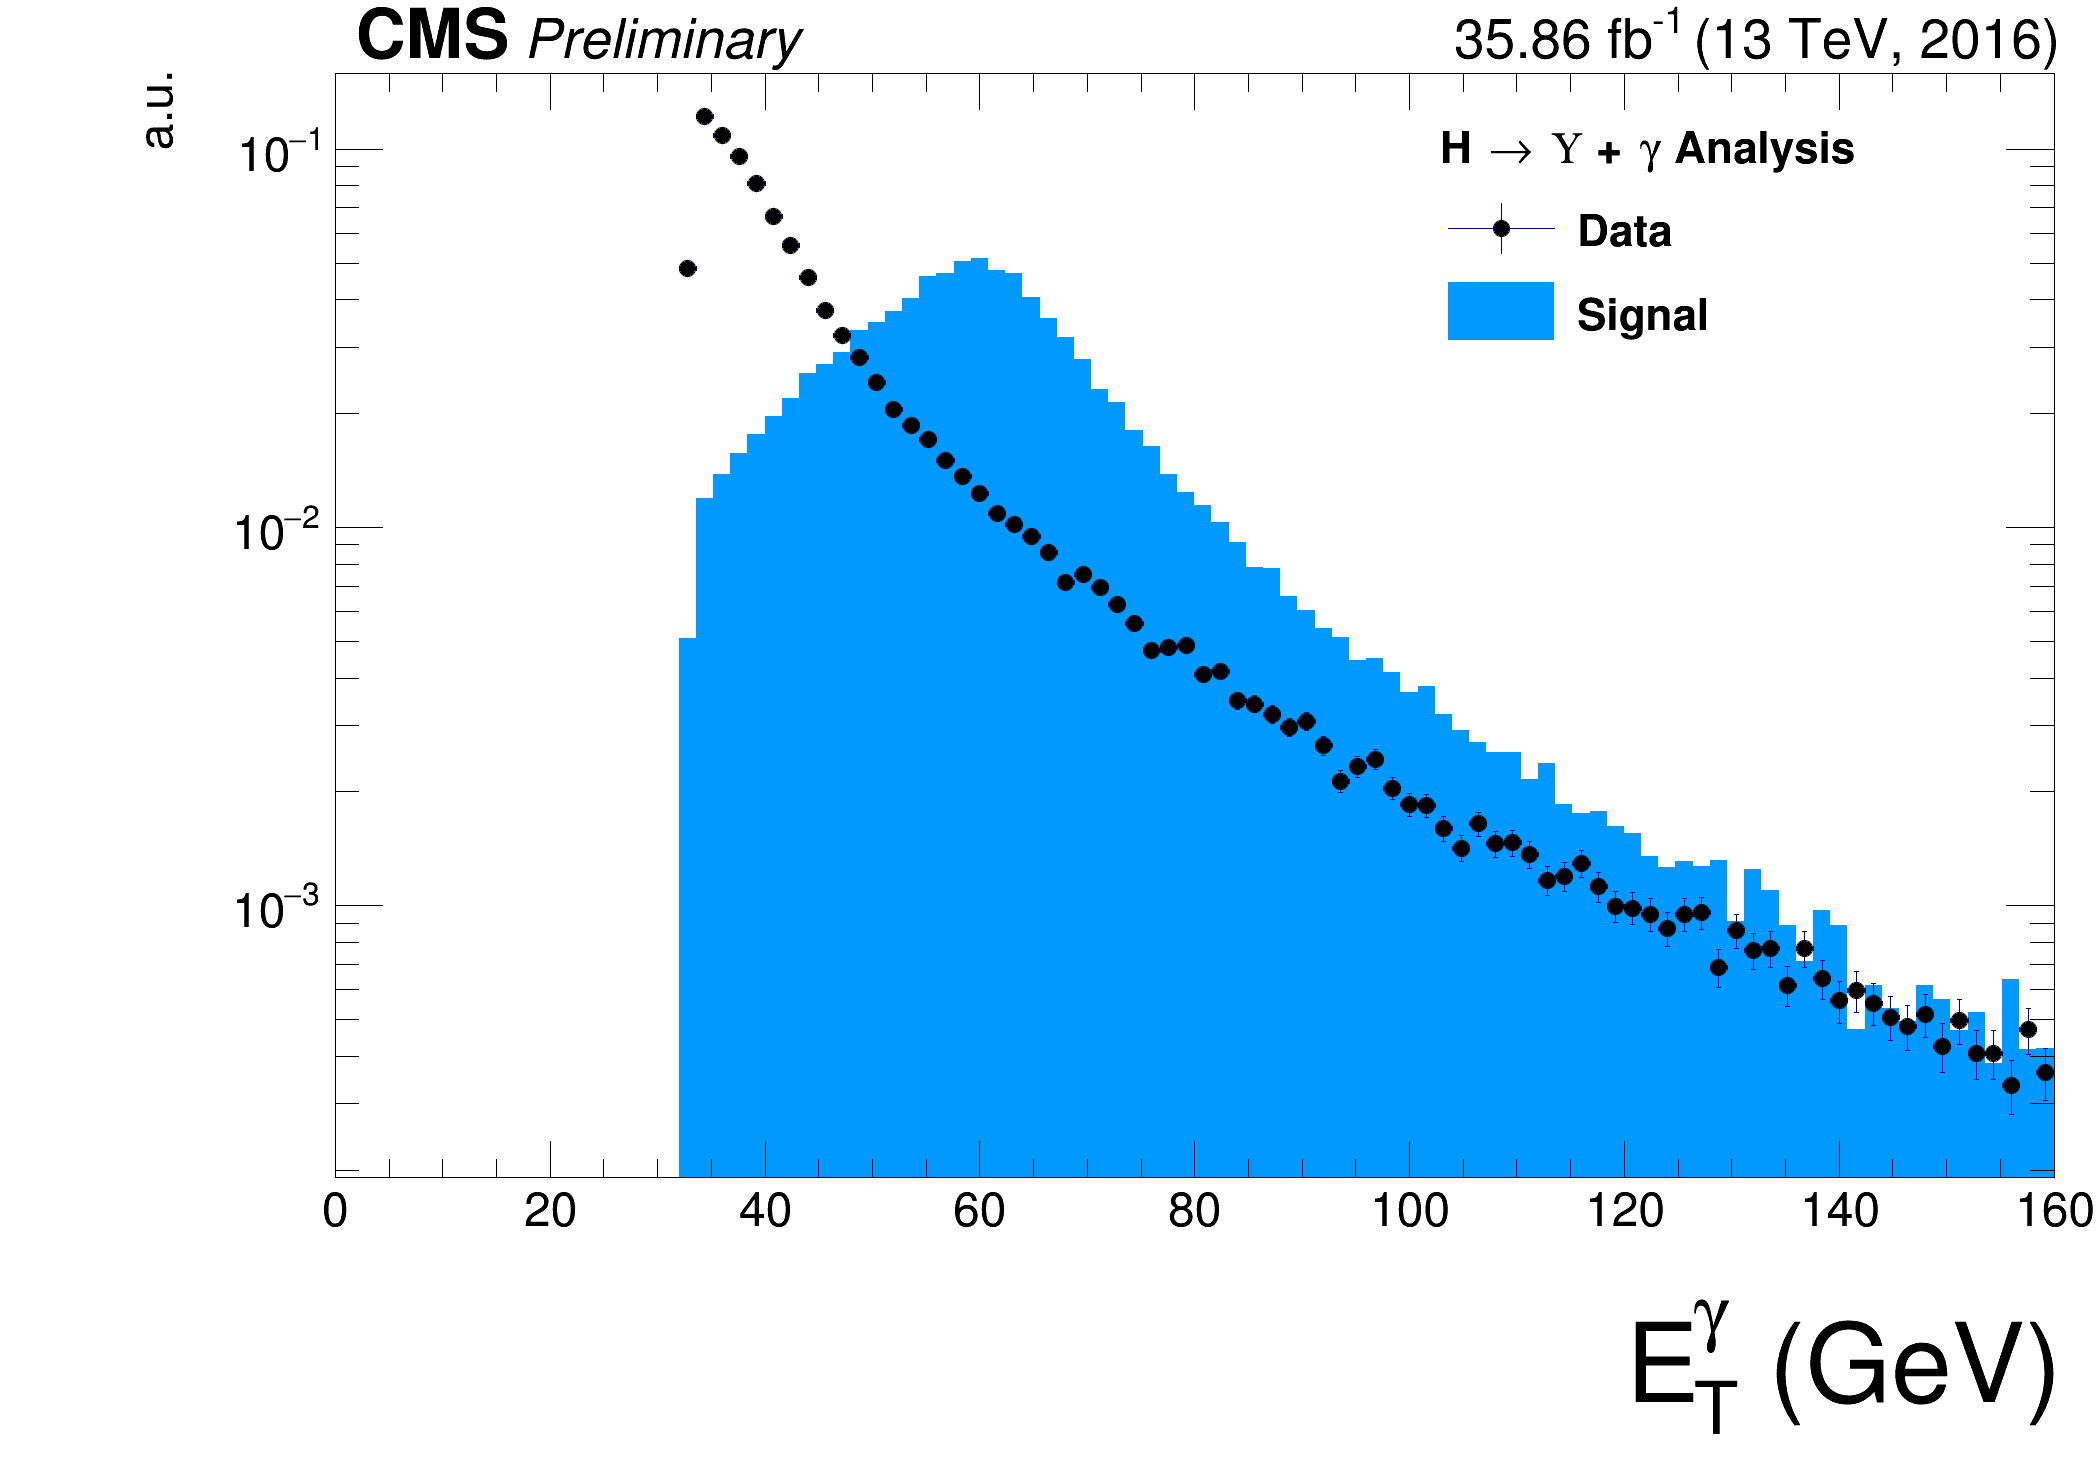
\includegraphics[width=0.45\textwidth]{figures_and_tables/outputPlots/HtoUpsilon_Cat0_ZZZZZ/au/data_x_mc/noKinCuts/h_noKin_Photon_pt}\hspace*{1.cm}
\end{center}\vspace*{-.5cm}
\caption{The \PT photon distributions from data and signal events for Higgs decaying into $\Upsilon(1S,2S,3S)$ + $\gamma$ Group I of selection cuts. The plot is normalized to the unit of area.}
\label{fig:pTPhoton_HtoUpsilon_Cat0}
\end{figure}


%%%%%%%$\eta$ Photon distributions for HtoUpsilon_Cat0
\begin{figure}[!htbp]
\begin{center}
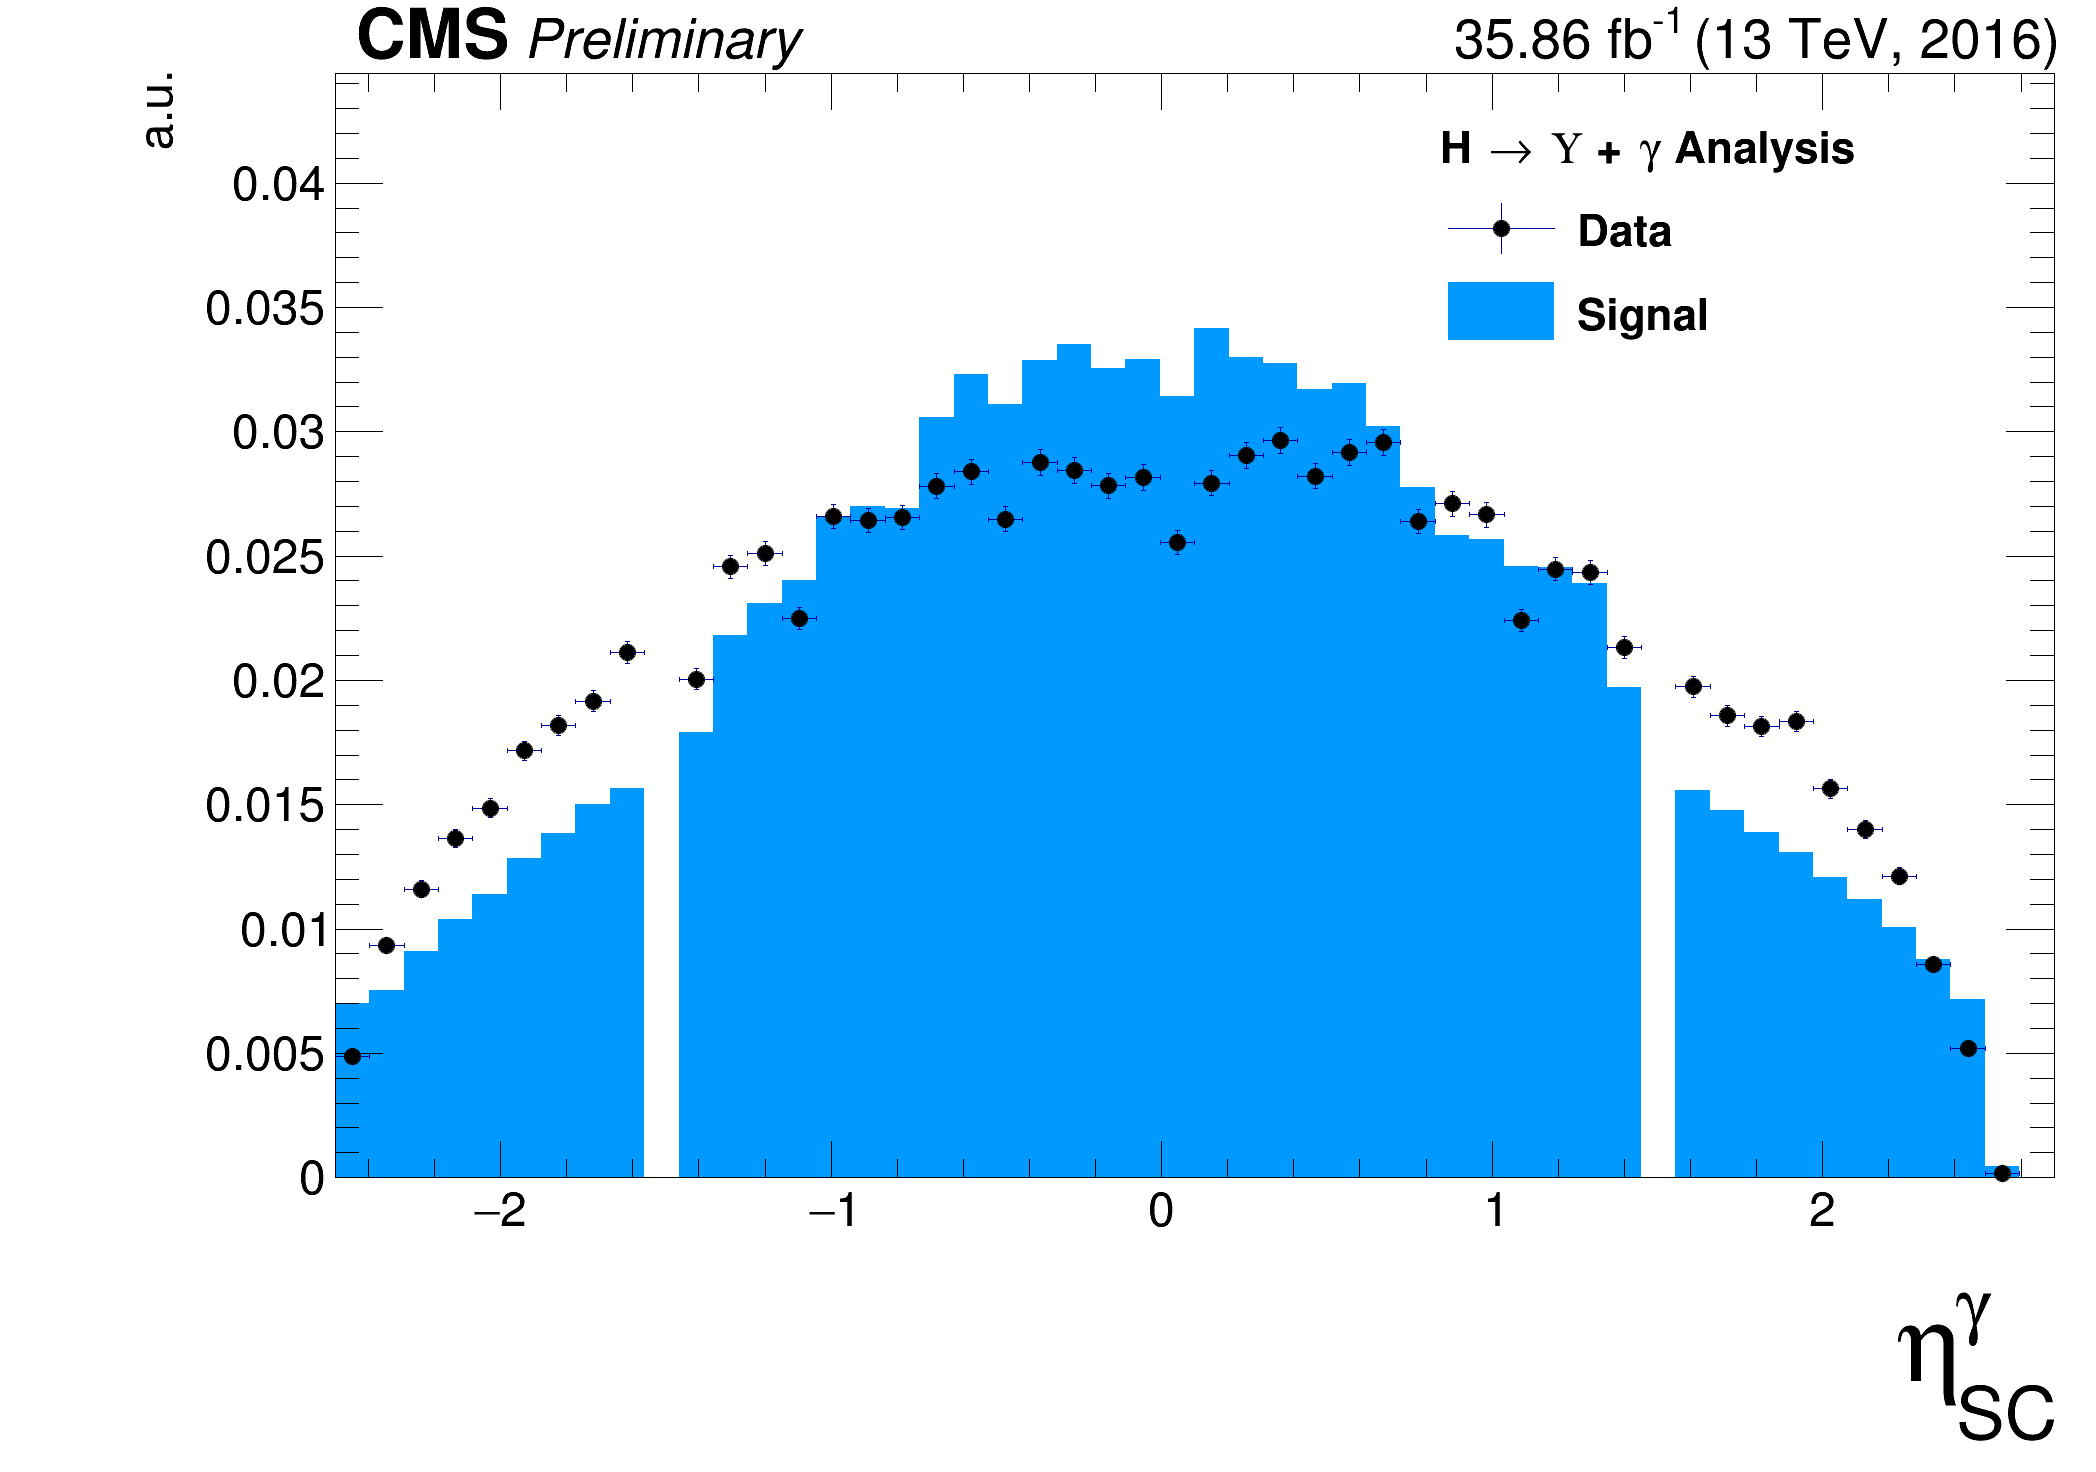
\includegraphics[width=0.45\textwidth]{figures_and_tables/outputPlots/HtoUpsilon_Cat0_ZZZZZ/au/data_x_mc/noKinCuts/h_noKin_Photon_eta}\hspace*{1.cm}
\end{center}\vspace*{-.5cm}
\caption{The $\eta$ photon distributions from data and signal events of Higgs decaying into $\Upsilon(1S,2S,3S)$ + $\gamma$ after Group I of selection cuts. The plot is normalized to the unit of area.}
\label{fig:etaPhoton_HtoUpsilon_Cat0}
\end{figure}

%%%%%%%%% $\phi$ Photon distributions for HtoUpsilon_Cat0
\begin{figure}[!htbp]
\begin{center}
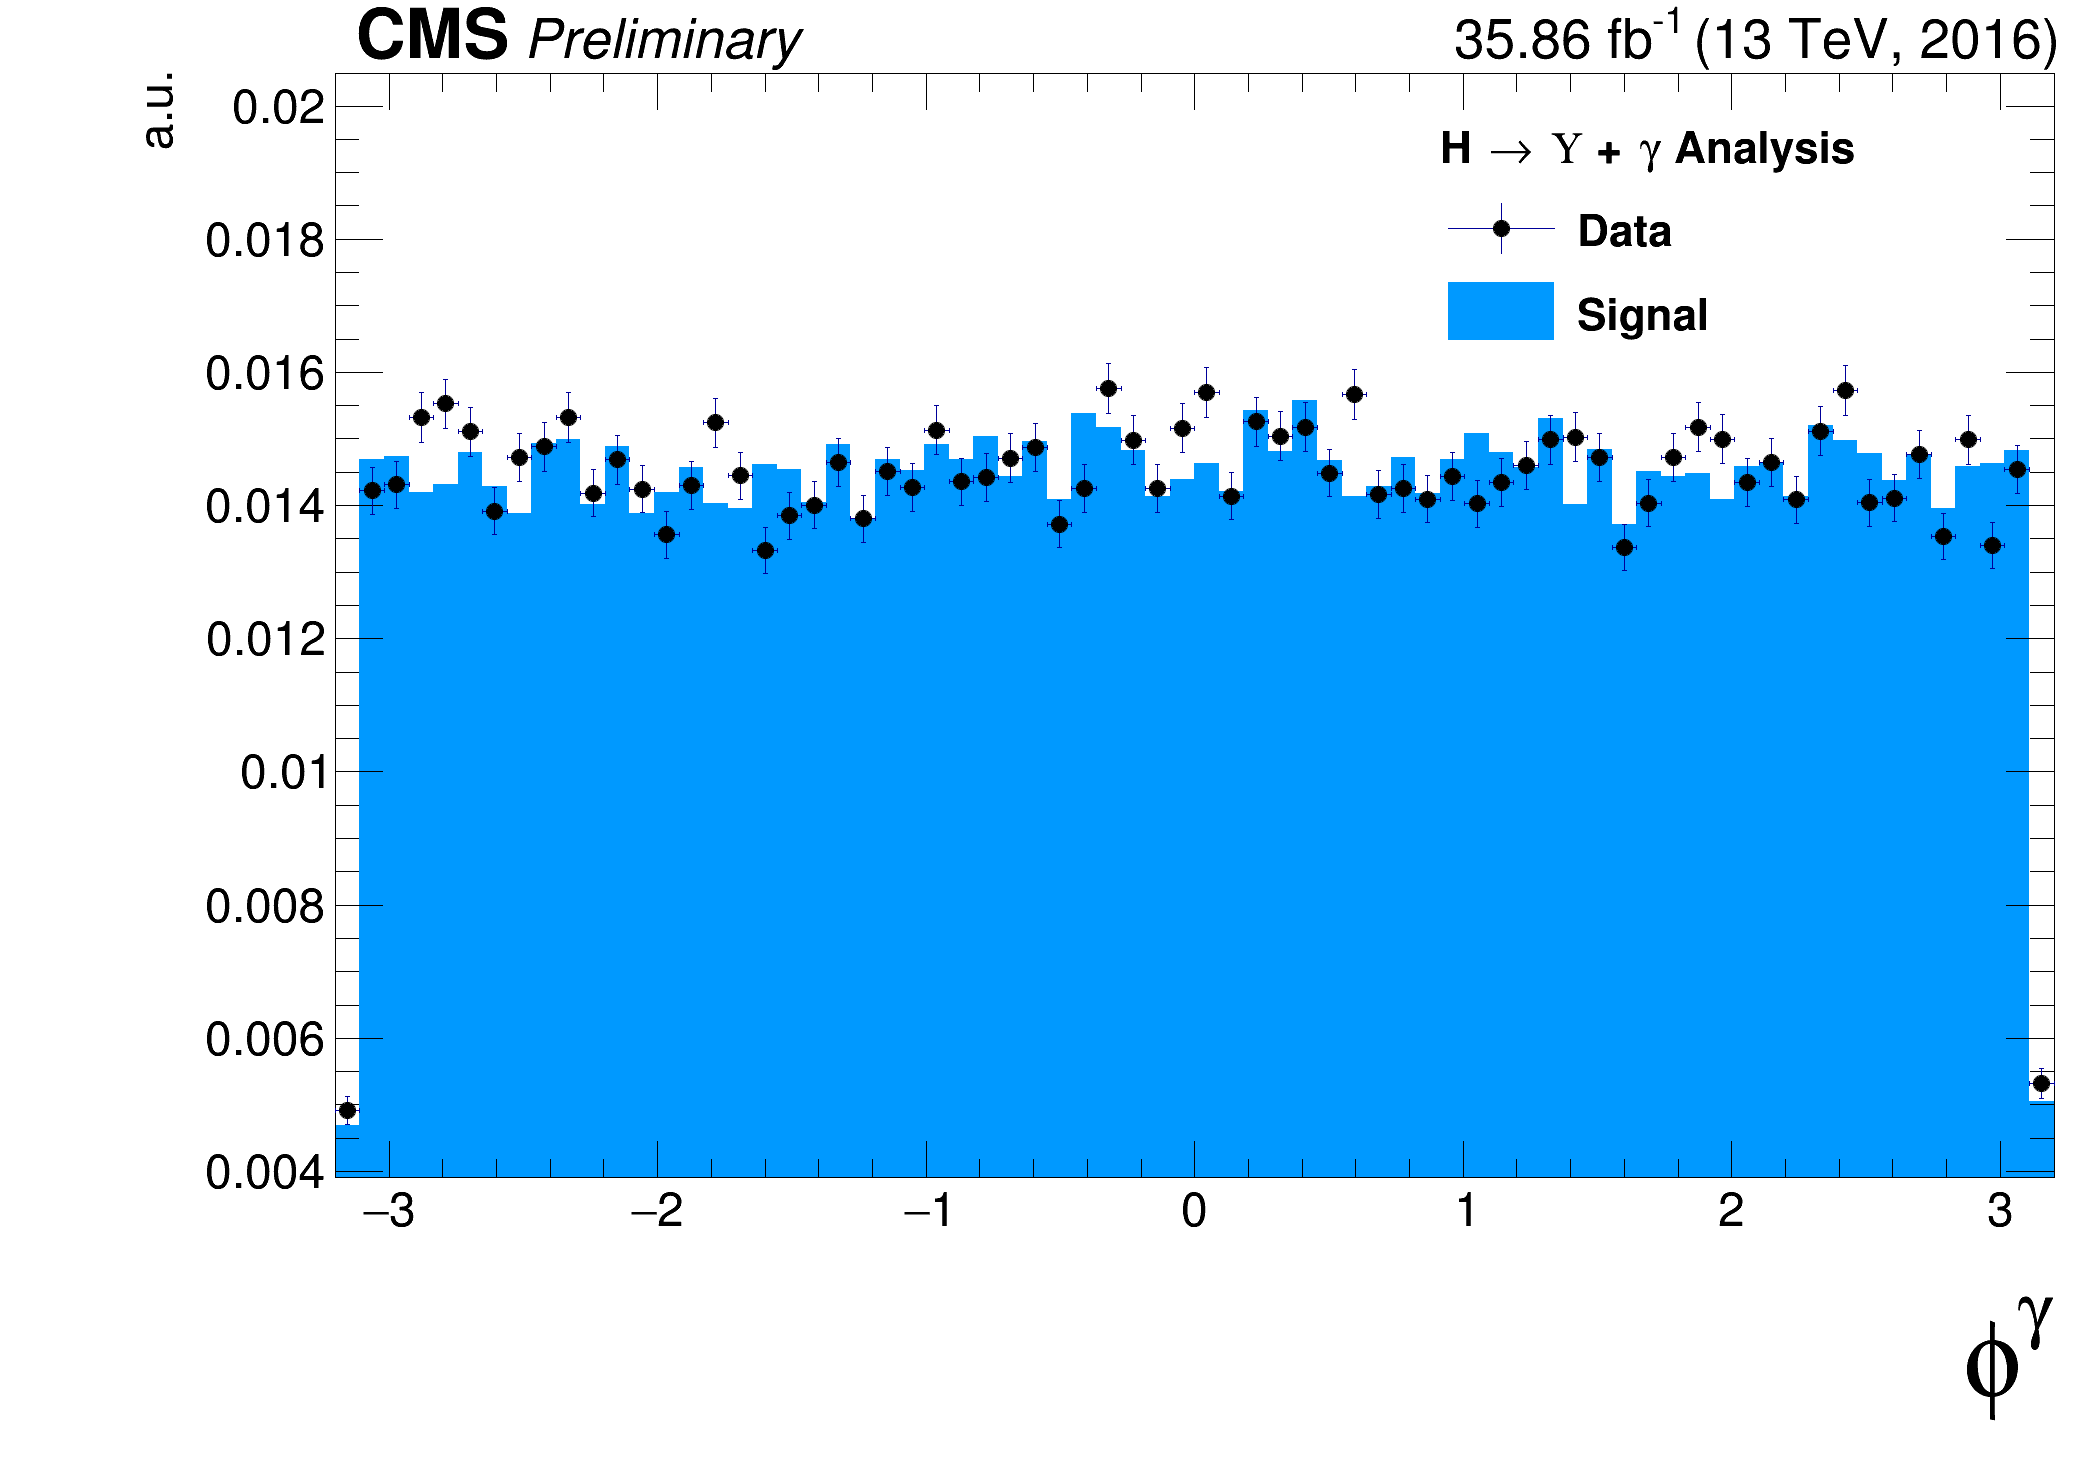
\includegraphics[width=0.45\textwidth]{figures_and_tables/outputPlots/HtoUpsilon_Cat0_ZZZZZ/au/data_x_mc/noKinCuts/h_noKin_Photon_phi}\hspace*{1.cm}
\end{center}\vspace*{-.5cm}
\caption{The $\phi$ photon distributions from data and signal events of Higgs decaying into $\Upsilon(1S,2S,3S)$ + $\gamma$ after Group I of selection cuts. The plot is normalized to the unit of area.}
\label{fig:phiPhoton_HtoUpsilon_Cat0}
\end{figure}

%%%%%%%%%%%%%
% Upsilon and Higgs boson
%%$\pT$ Upsilon_and_Higgs distributions for HtoUpsilon_Cat0
\begin{figure}[!htbp]
\begin{center}
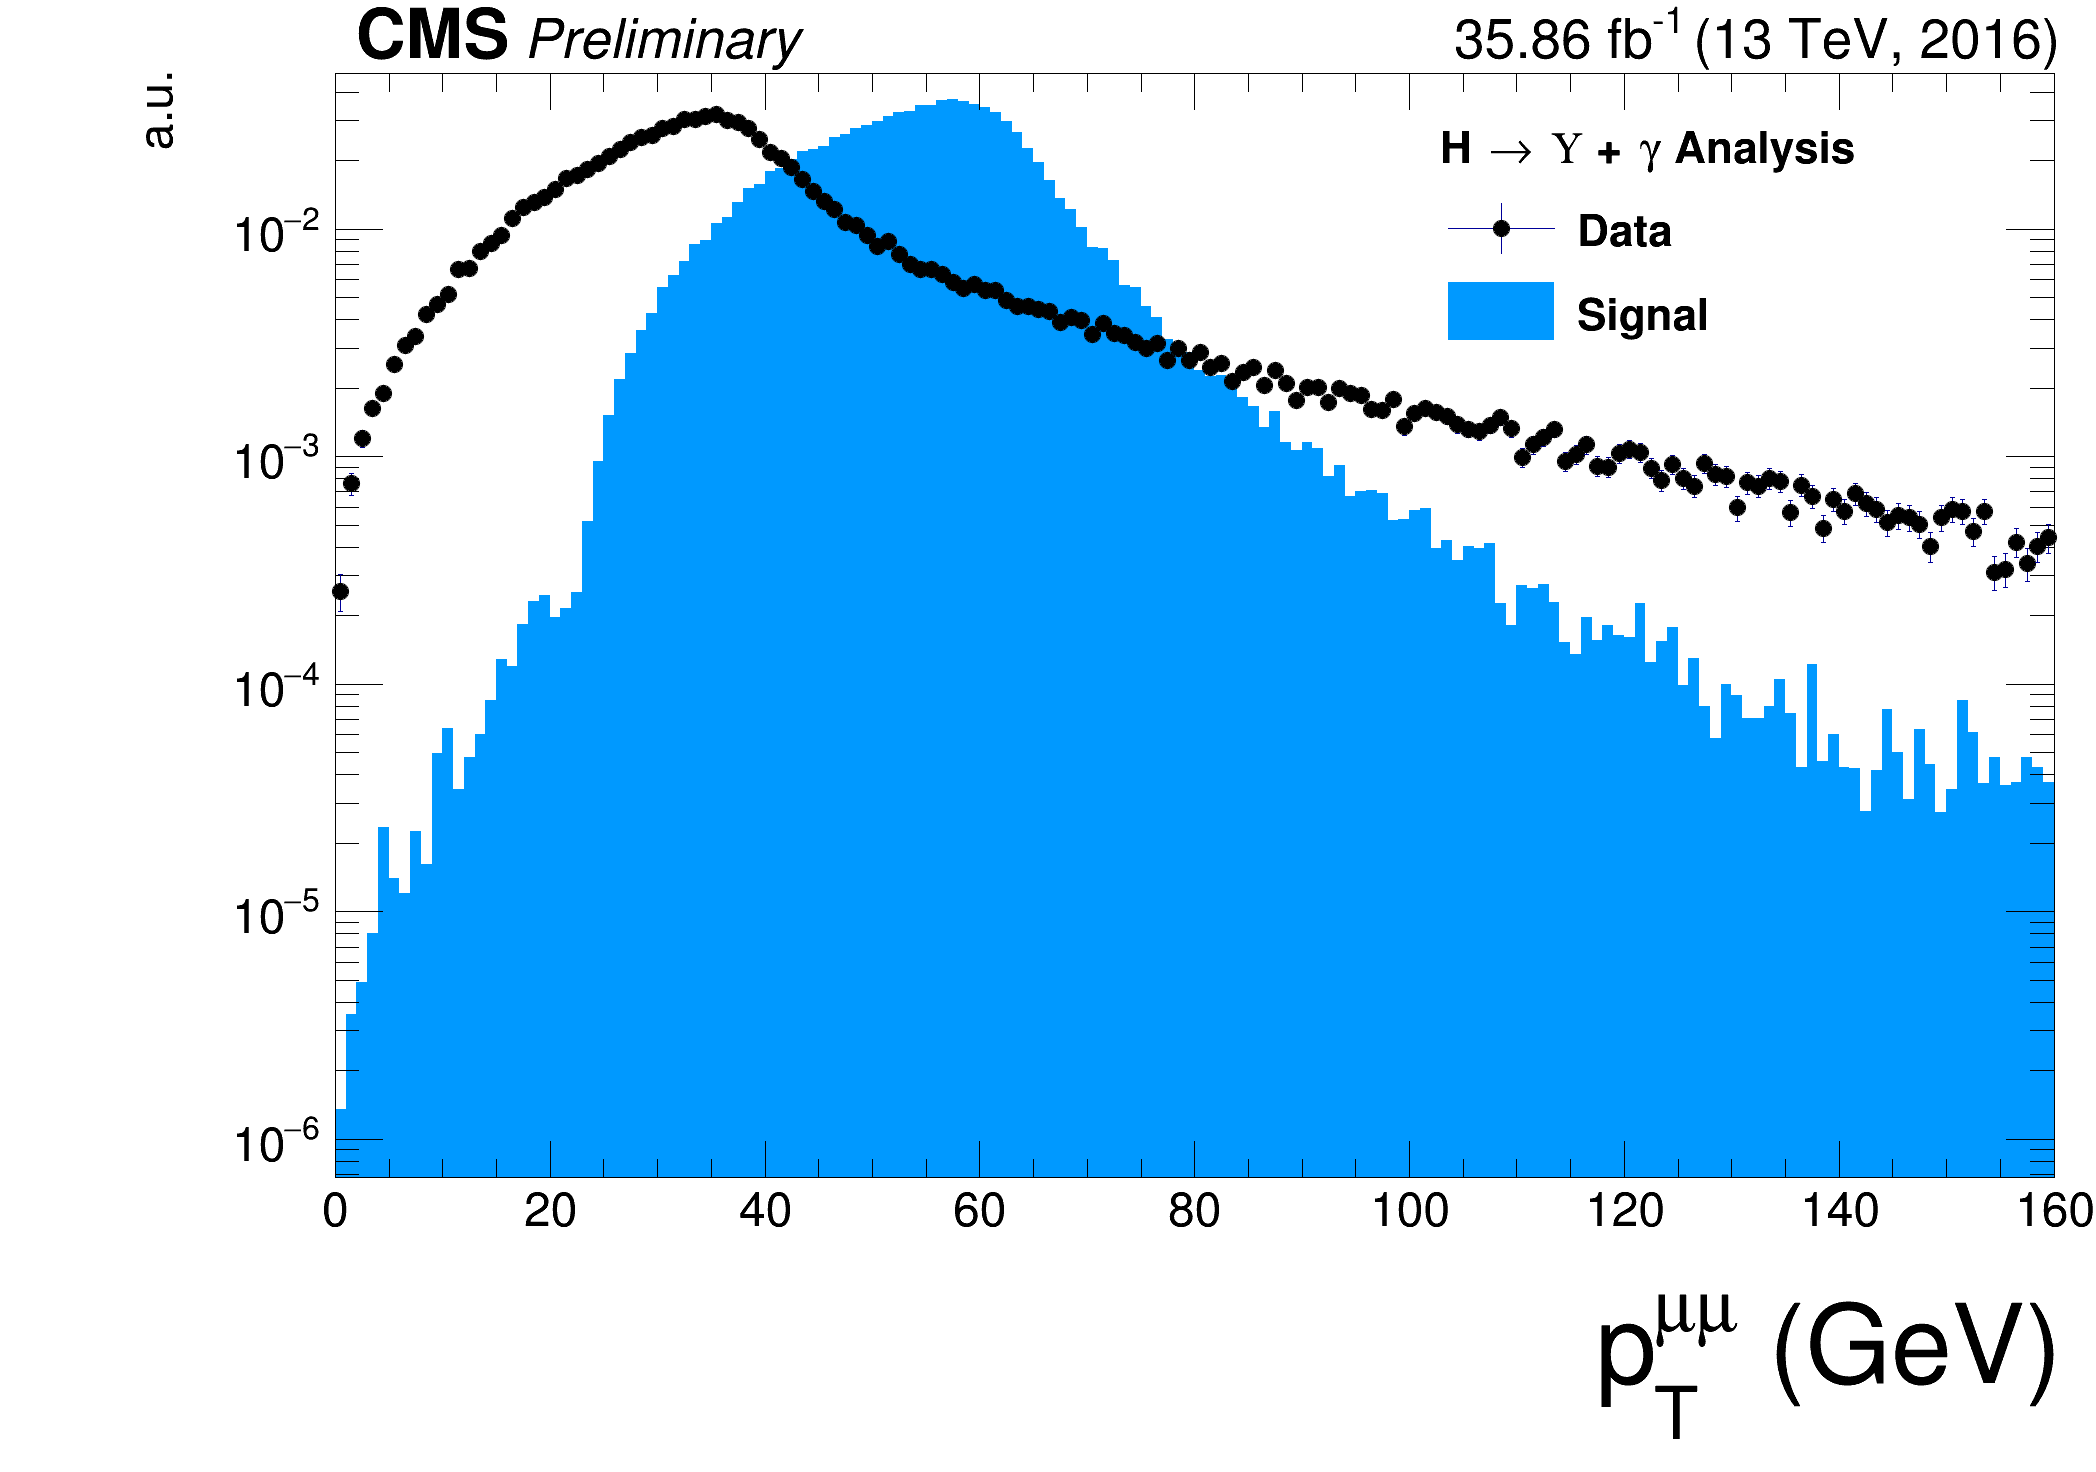
\includegraphics[width=0.45\textwidth]{figures_and_tables/outputPlots/HtoUpsilon_Cat0_ZZZZZ/au/data_x_mc/noKinCuts/h_noKin_Upsilon_Pt}\hspace*{1.cm}
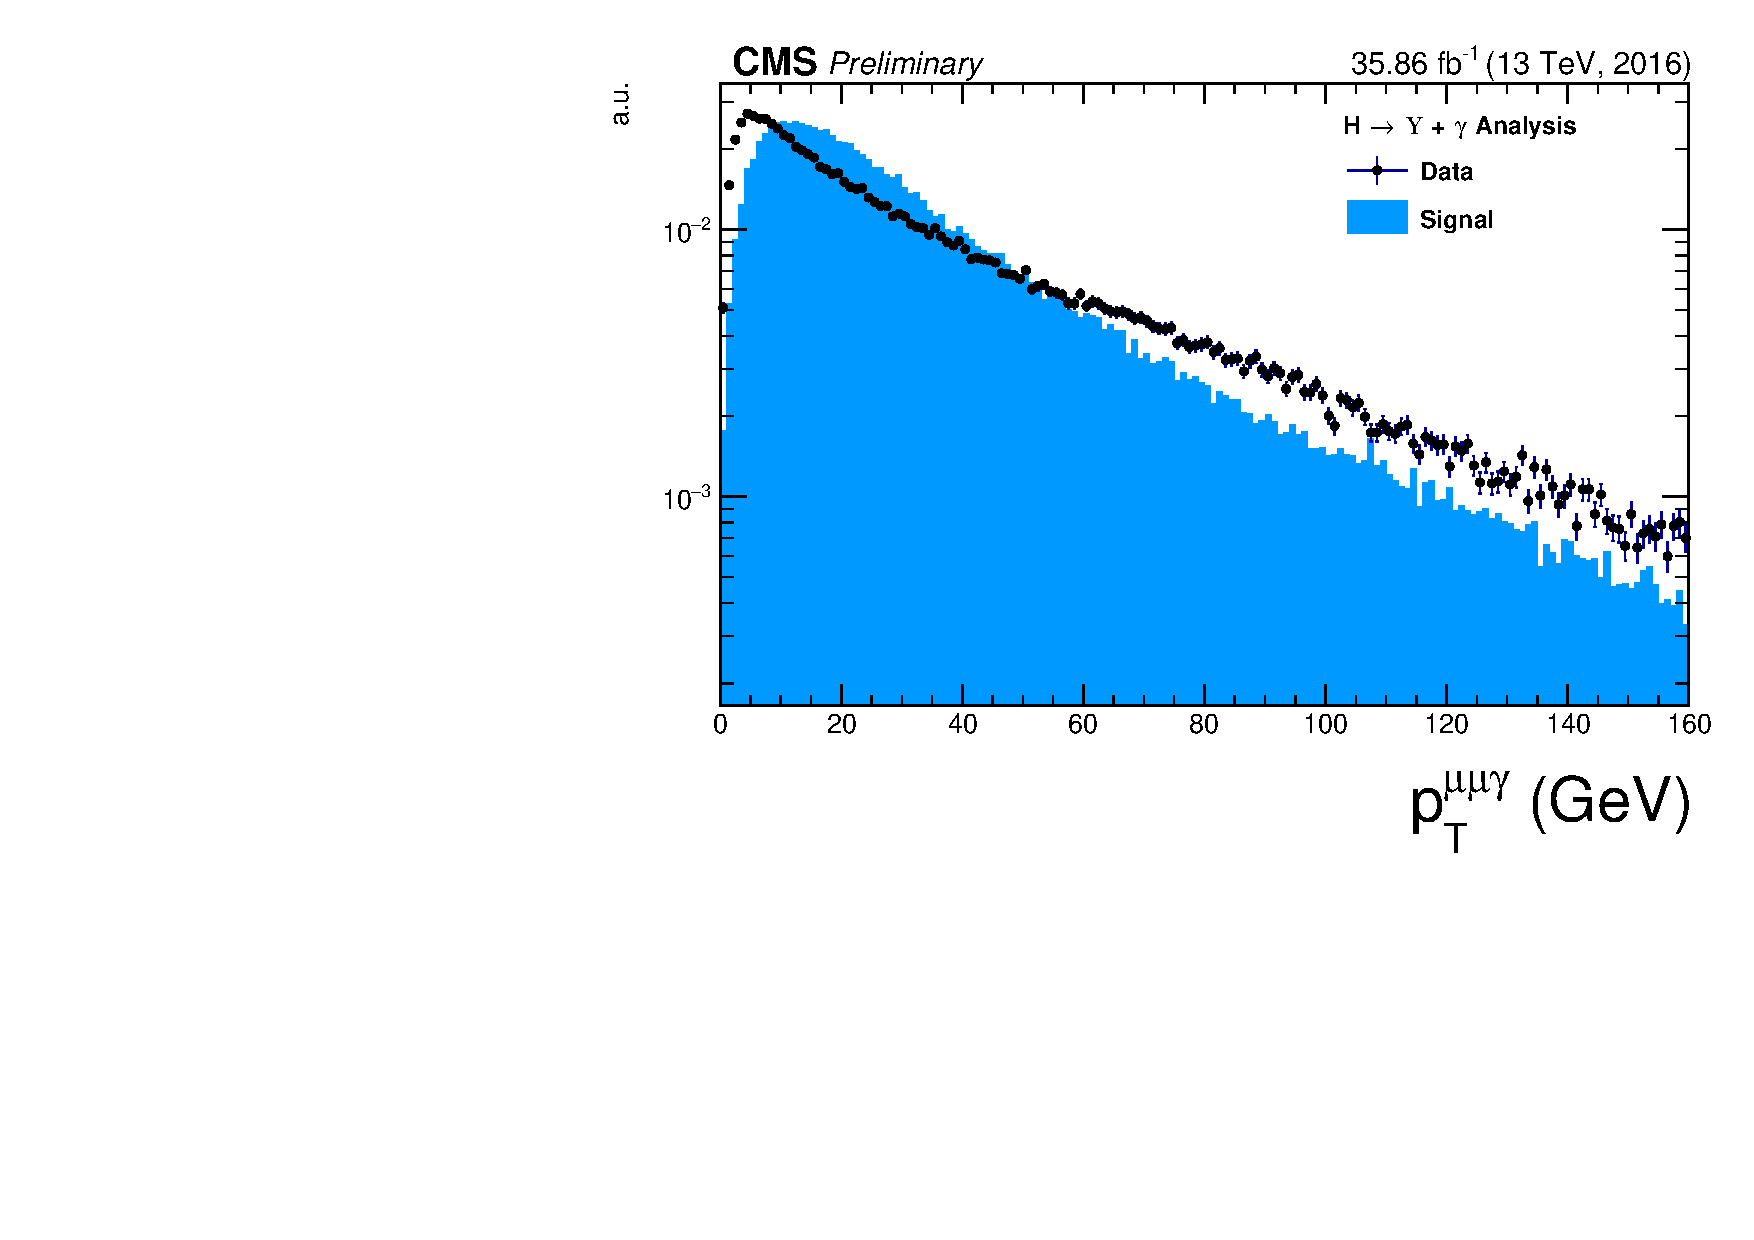
\includegraphics[width=0.45\textwidth]{figures_and_tables/outputPlots/HtoUpsilon_Cat0_ZZZZZ/au/data_x_mc/noKinCuts/h_noKin_Z_Pt}
\end{center}\vspace*{-.5cm}
\caption{The \PT distributions for $\Upsilon(1S,2S,3S)$ in the left and for Higgs in the right from data and signal events for Higgs decaying into $\Upsilon(1S,2S,3S)$ + $\gamma$ after Group I of selection cuts. The plots are normalized to the unit of area. The black dots are data collect by CMS while the blue distribution is related only to the signal Monte-Carlo generated samples.}
\label{fig:pTUpsilon_and_Higgs_HtoUpsilon_Cat0}
\end{figure}


%%%%%%%$\eta$ Upsilon_and_Higgs distributions for HtoUpsilon_Cat0
\begin{figure}[!htbp]
\begin{center}
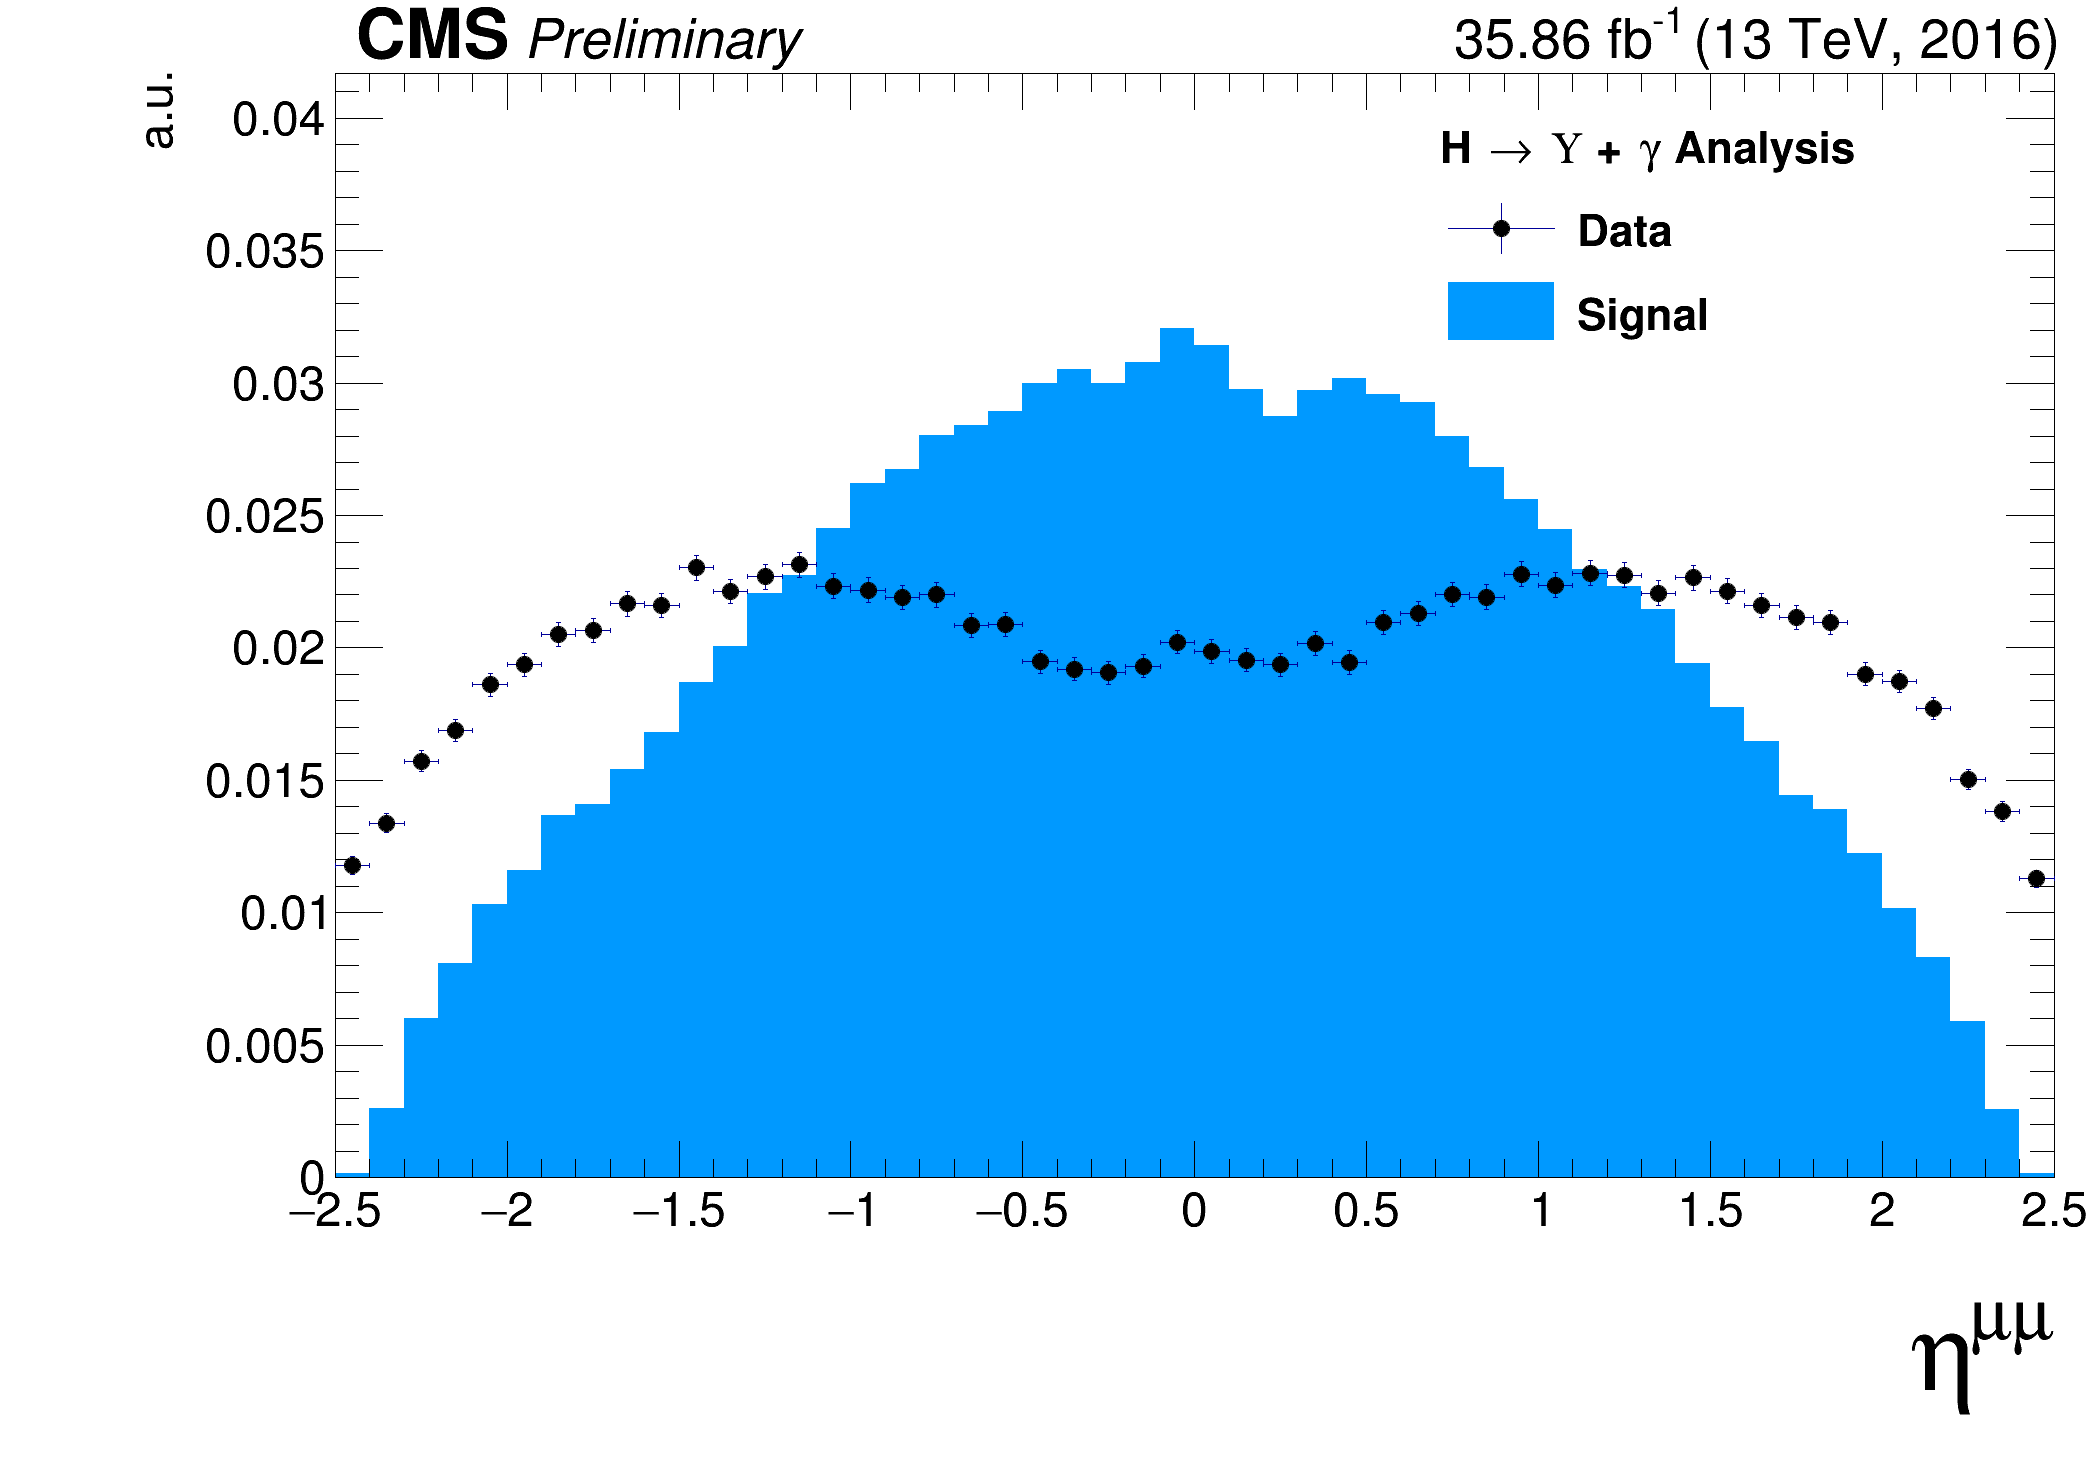
\includegraphics[width=0.45\textwidth]{figures_and_tables/outputPlots/HtoUpsilon_Cat0_ZZZZZ/au/data_x_mc/noKinCuts/h_noKin_Upsilon_eta}\hspace*{1.cm}
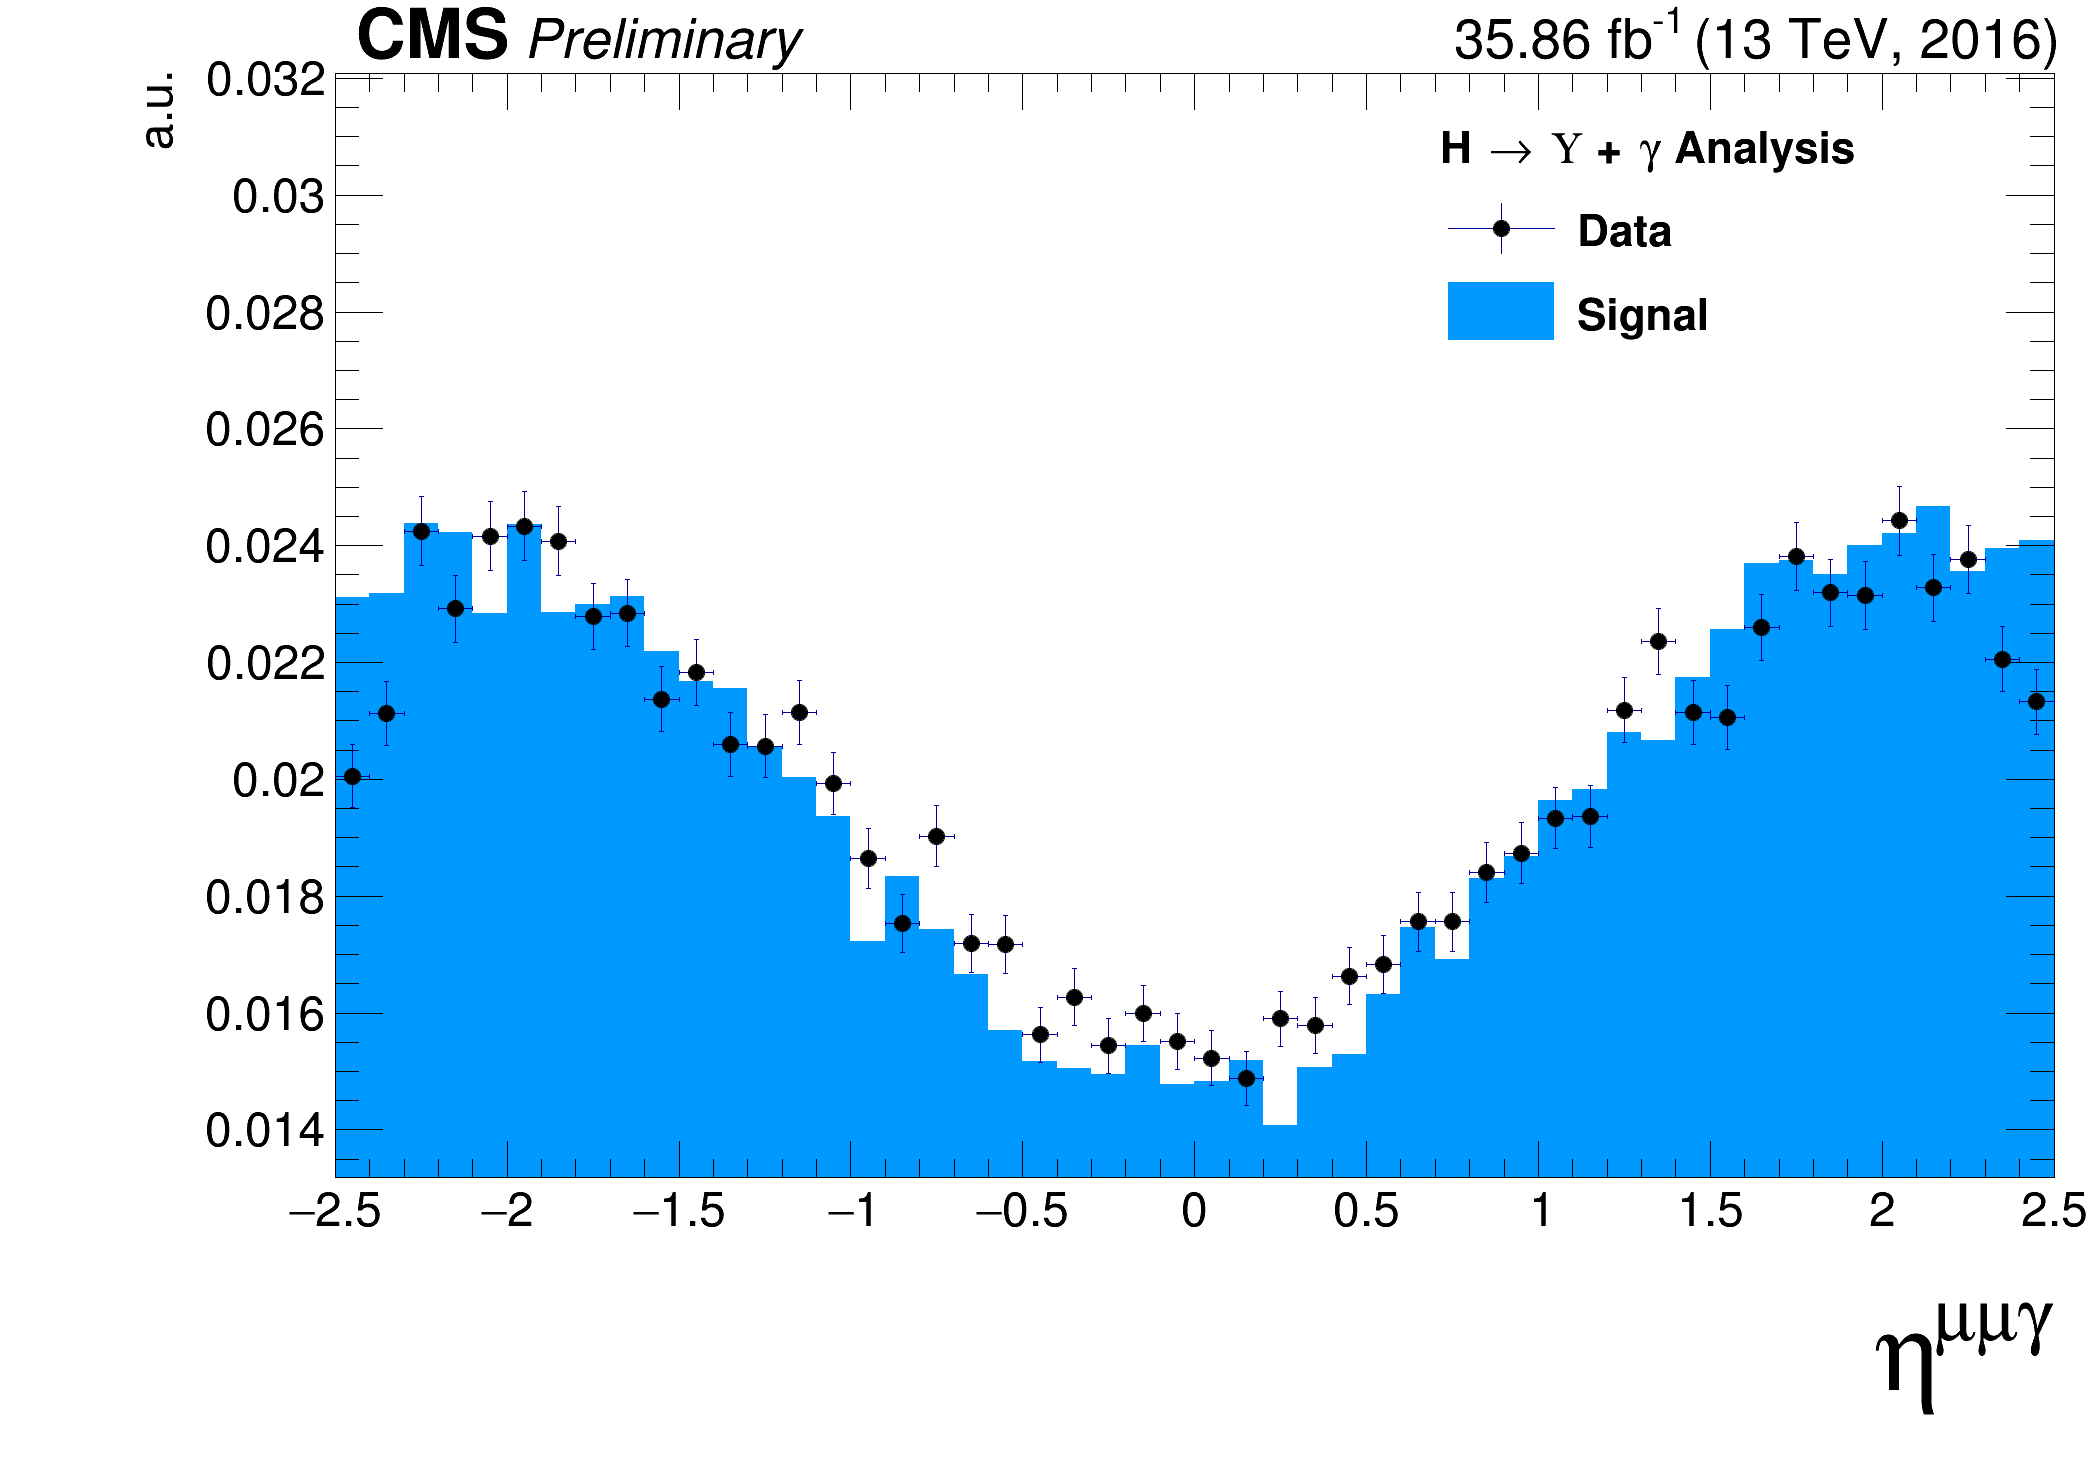
\includegraphics[width=0.45\textwidth]{figures_and_tables/outputPlots/HtoUpsilon_Cat0_ZZZZZ/au/data_x_mc/noKinCuts/h_noKin_Z_eta}
\end{center}\vspace*{-.5cm}
\caption{The $\eta$ distributions for $\Upsilon(1S,2S,3S)$ in the left and for Higgs in the right from data and signal events for Higgs decaying into $\Upsilon(1S,2S,3S)$ + $\gamma$ after Group I of selection cuts. The plots are normalized to the unit of area. The black dots are data collect by CMS while the blue distribution is related only to the signal Monte-Carlo generated samples.}
\label{fig:etaUpsilon_and_Higgs_HtoUpsilon_Cat0}
\end{figure}

%%%%%%%%% $\phi$ Upsilon_and_Higgsdistributions for HtoUpsilon_Cat0
\begin{figure}[!htbp]
\begin{center}
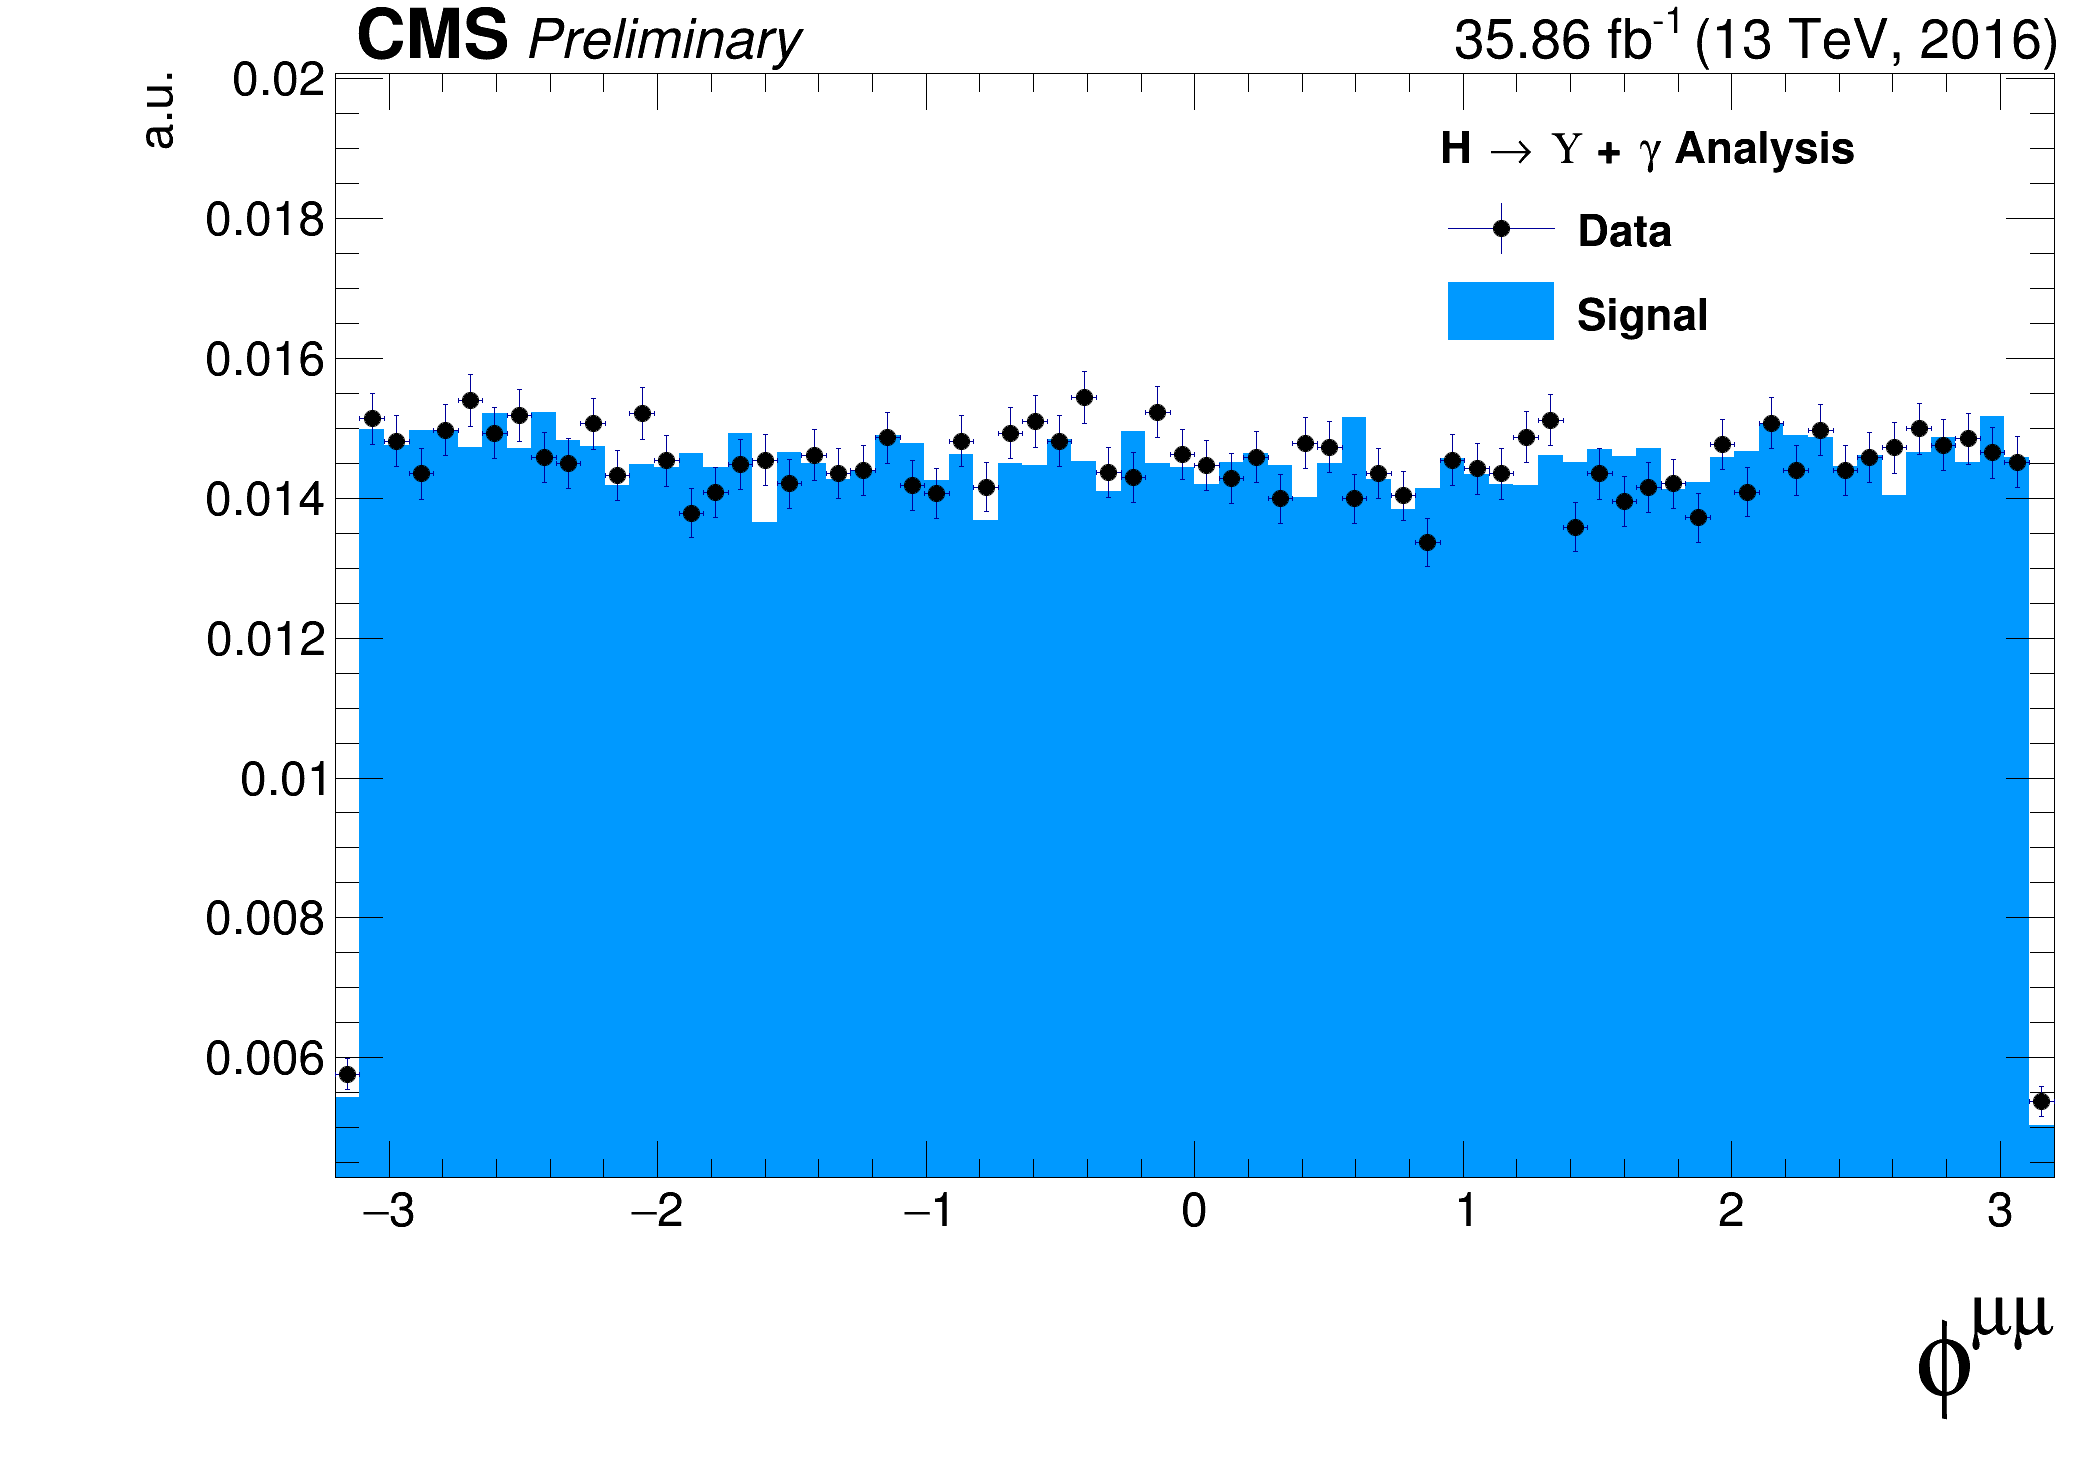
\includegraphics[width=0.45\textwidth]{figures_and_tables/outputPlots/HtoUpsilon_Cat0_ZZZZZ/au/data_x_mc/noKinCuts/h_noKin_Upsilon_phi}\hspace*{1.cm}
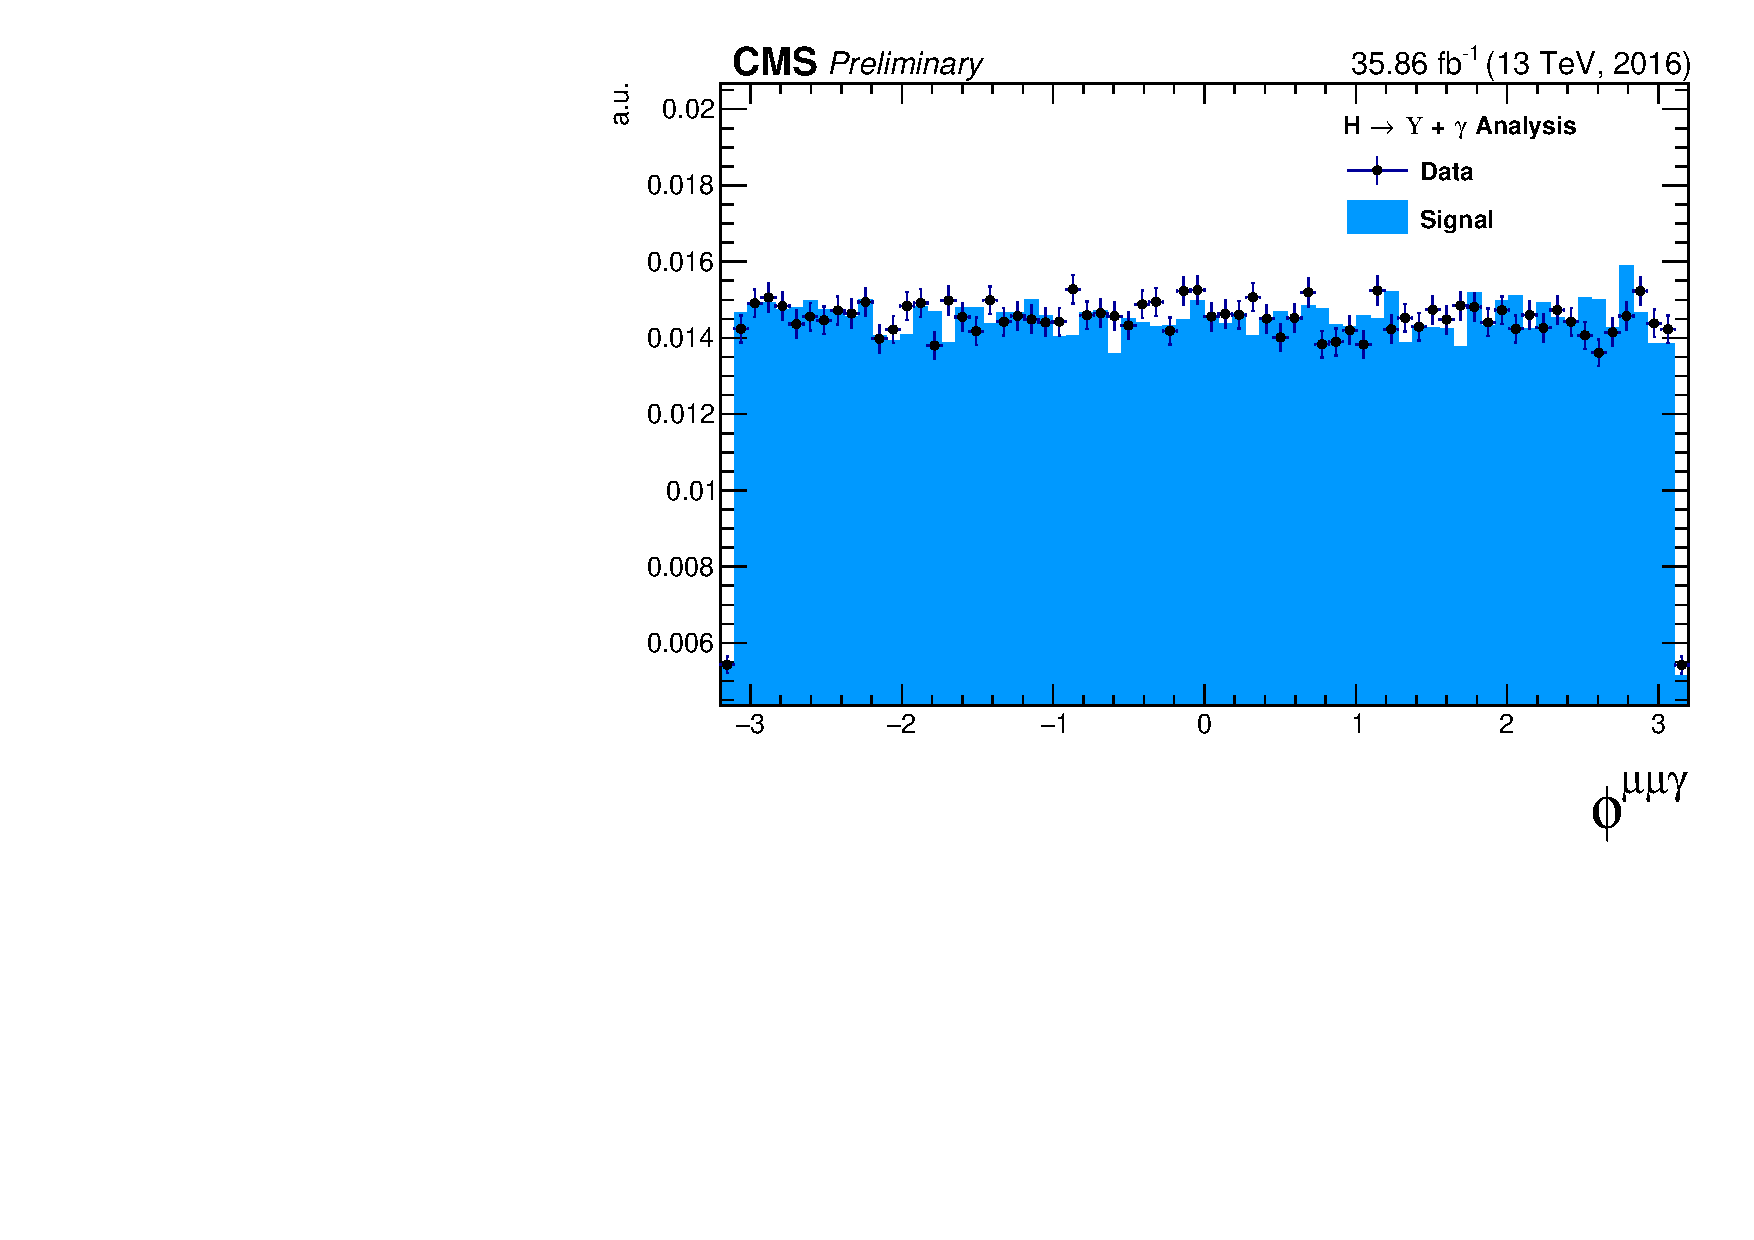
\includegraphics[width=0.45\textwidth]{figures_and_tables/outputPlots/HtoUpsilon_Cat0_ZZZZZ/au/data_x_mc/noKinCuts/h_noKin_Z_phi}
\end{center}\vspace*{-.5cm}
\caption{The $\phi$ distributions for $\Upsilon(1S,2S,3S)$ in the left and for Higgs in the right from data and signal events for Higgs decaying into $\Upsilon(1S,2S,3S)$ + $\gamma$ after Group I of selection cuts. The plots are normalized to the unit of area. The black dots are data collect by CMS while the blue distribution is related only to the signal Monte-Carlo generated samples.}
\label{fig:phiUpsilon_and_Higgs_HtoUpsilon_Cat0}
\end{figure}

%%%%%%%%%%%%

%%%%%%%%%%%%%
% kin cuts
%% delta R -  mu x photon distributions for HtoUpsilon_Cat0
\begin{figure}[!htbp]
\begin{center}
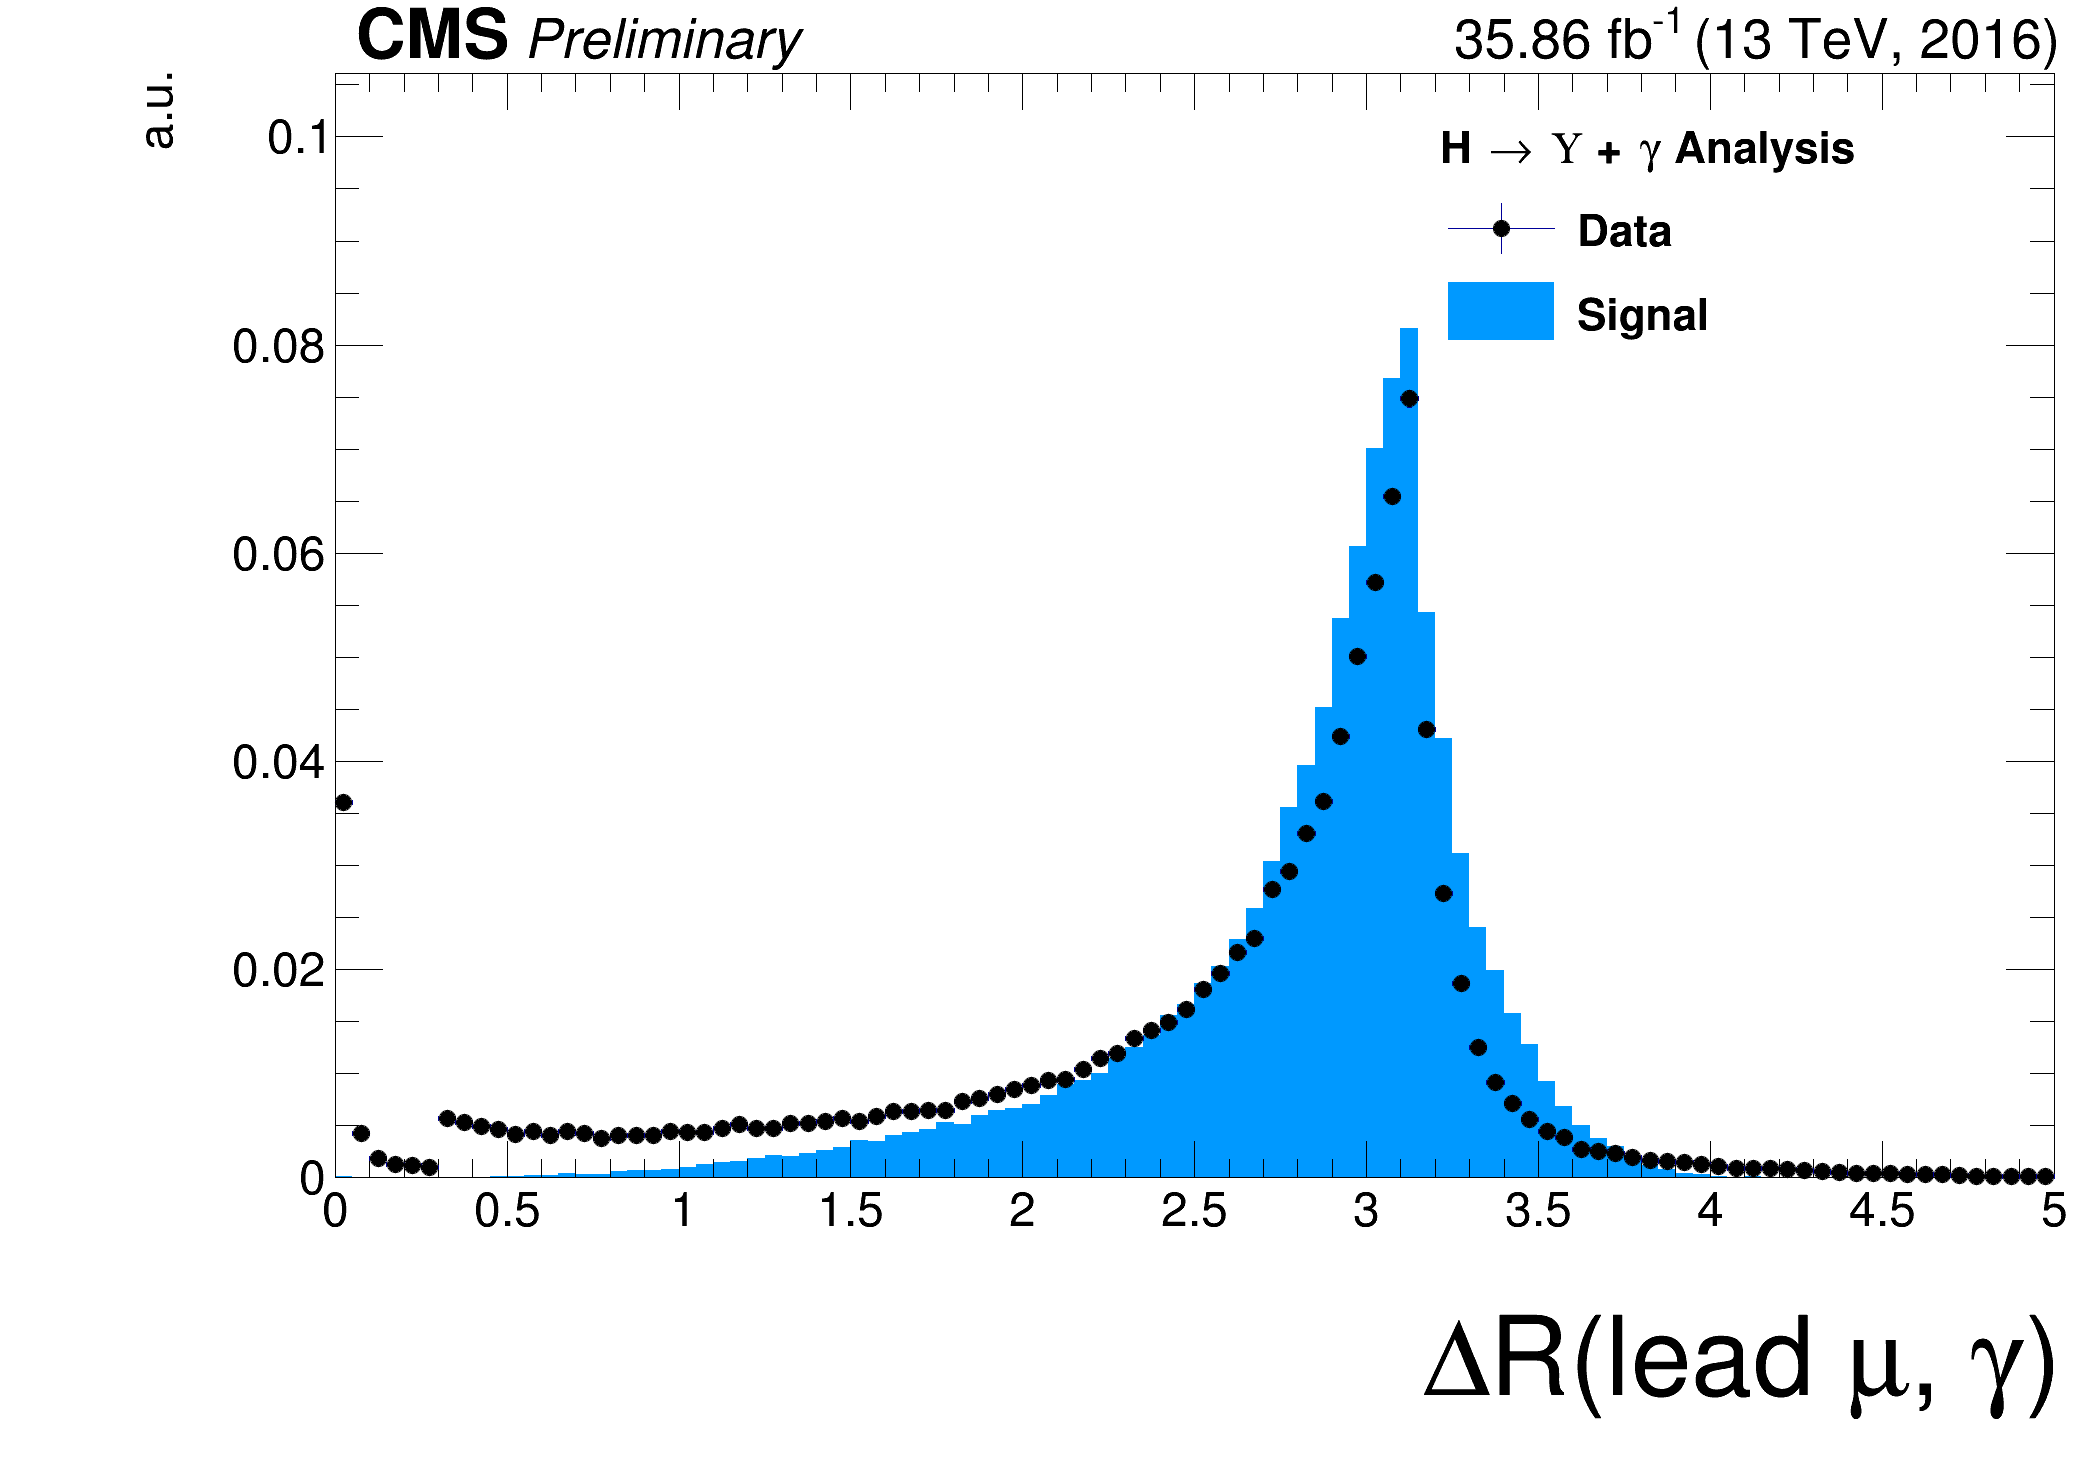
\includegraphics[width=0.45\textwidth]{figures_and_tables/outputPlots/HtoUpsilon_Cat0_ZZZZZ/au/data_x_mc/noKinCuts/h_noKin_deltaR_Leading_Photon}\hspace*{1.cm}
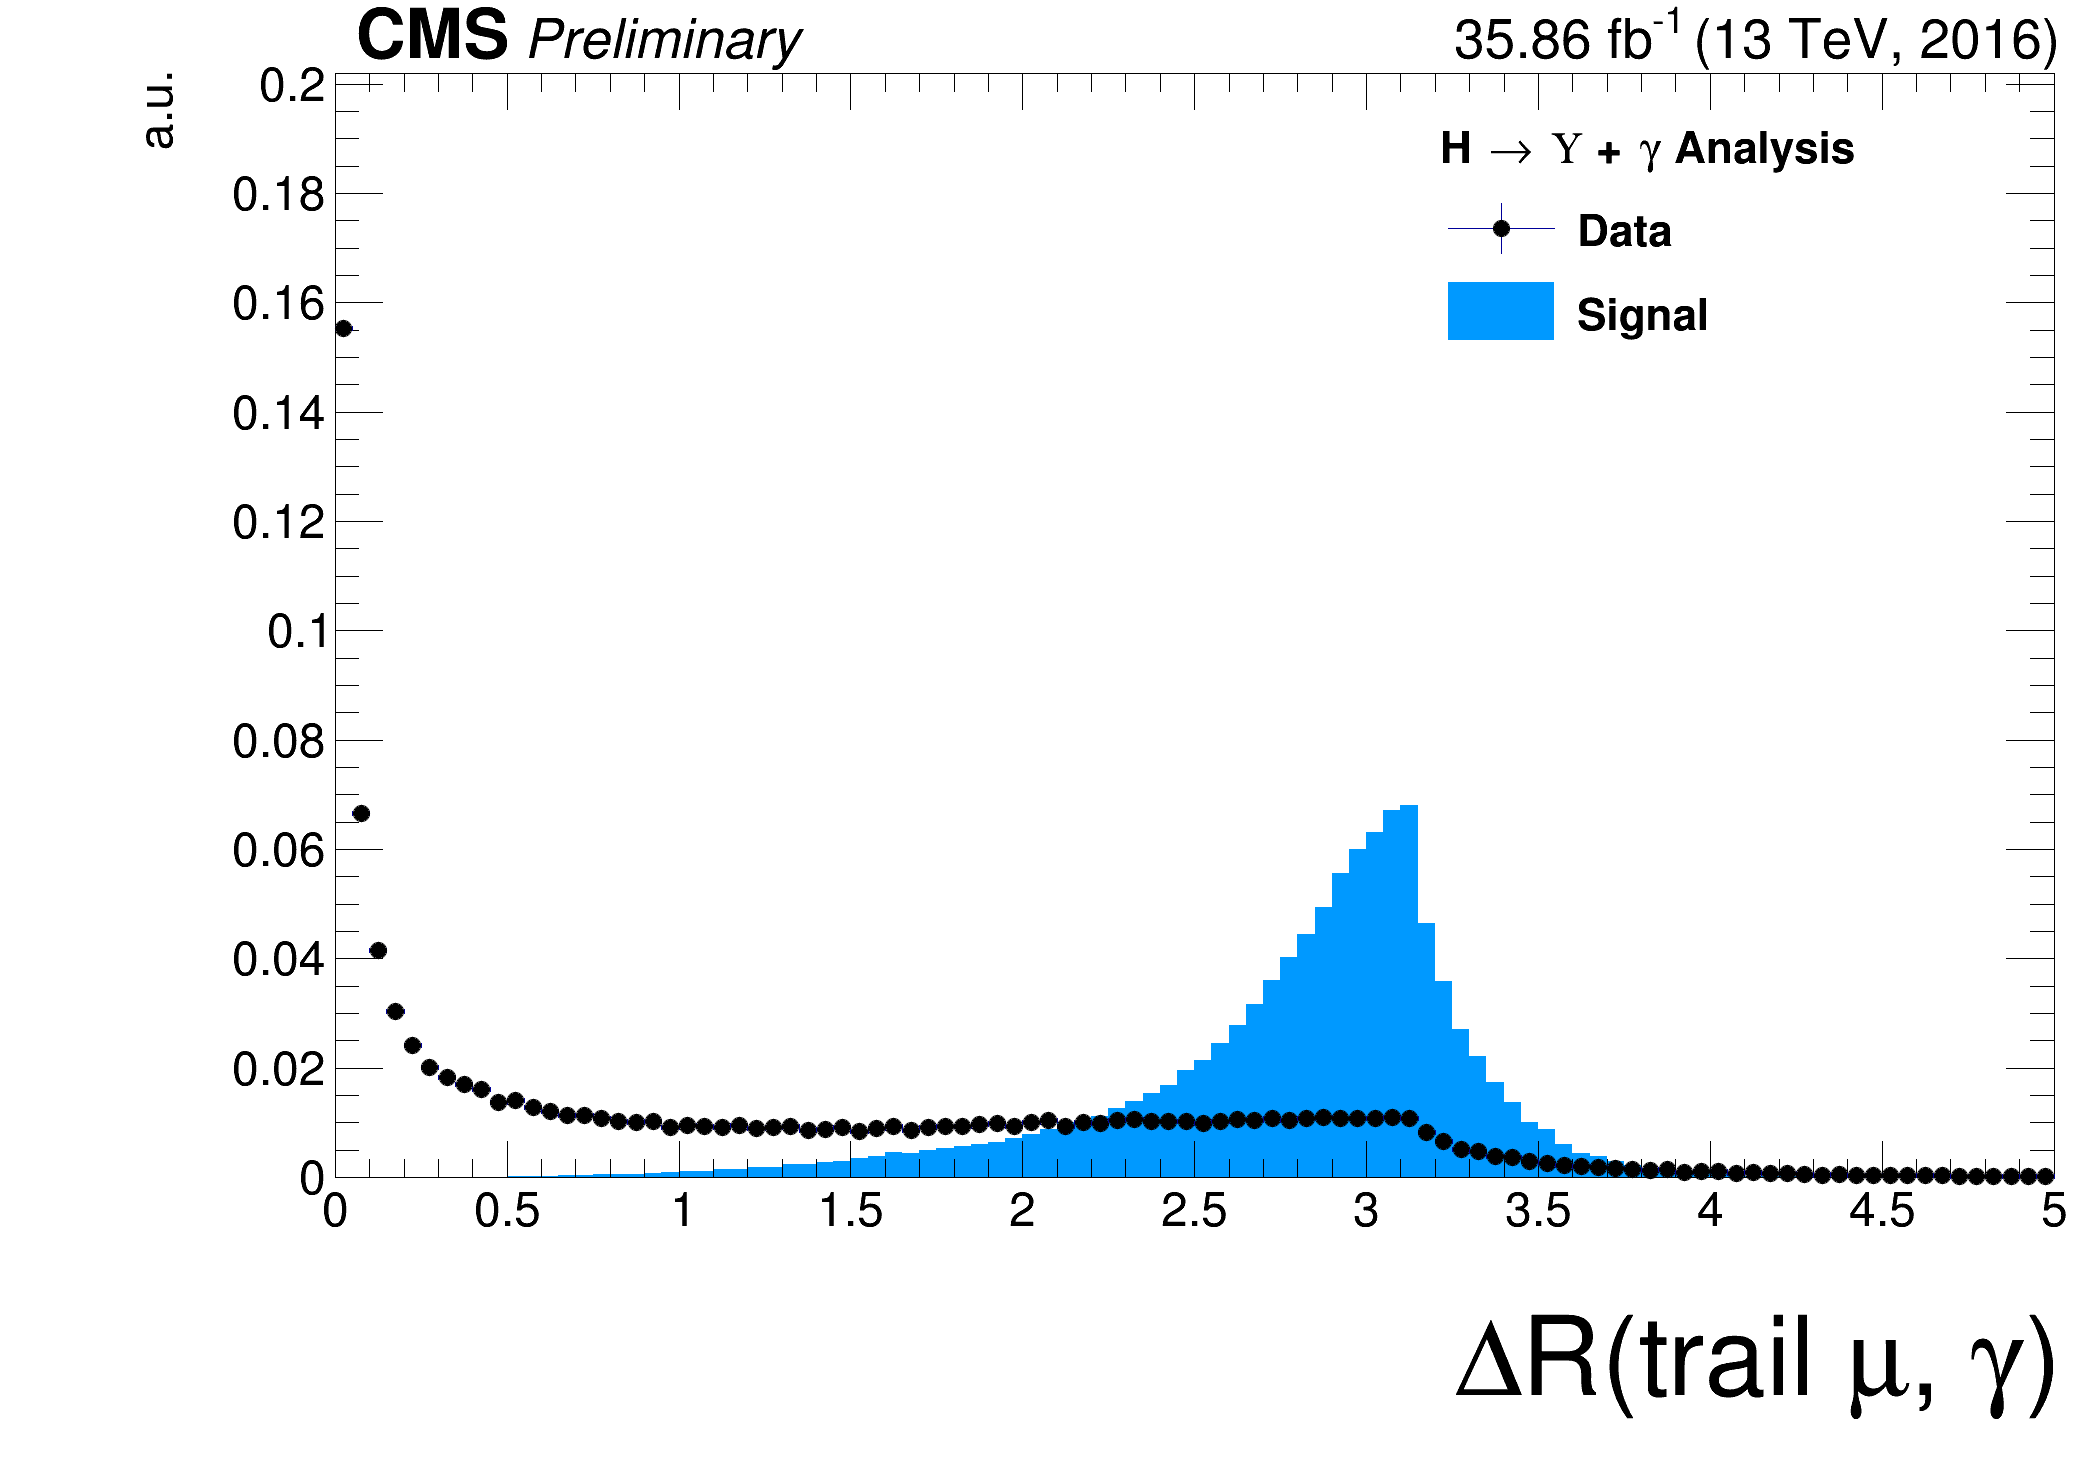
\includegraphics[width=0.45\textwidth]{figures_and_tables/outputPlots/HtoUpsilon_Cat0_ZZZZZ/au/data_x_mc/noKinCuts/h_noKin_deltaR_Trailing_Photon}\end{center}\vspace*{-.5cm}
\caption{The $\Delta R$ distributions between the photon and the leading muon (left) and the trailing muon (right) for Higgs decaying into $\Upsilon(1S,2S,3S)$ + $\gamma$ from data and signal events after Group I of selection cuts. The plots are normalized to the unit of area. The black dots are data collect by CMS while the blue distribution is related only to the signal Monte-Carlo generated samples.}
\label{fig:deltaR_HtoUpsilon_Cat0}
\end{figure}

%% delta R and Delta Phi -  MuMu x photon distributions for HtoUpsilon_Cat0
\begin{figure}[!htbp]
\begin{center}
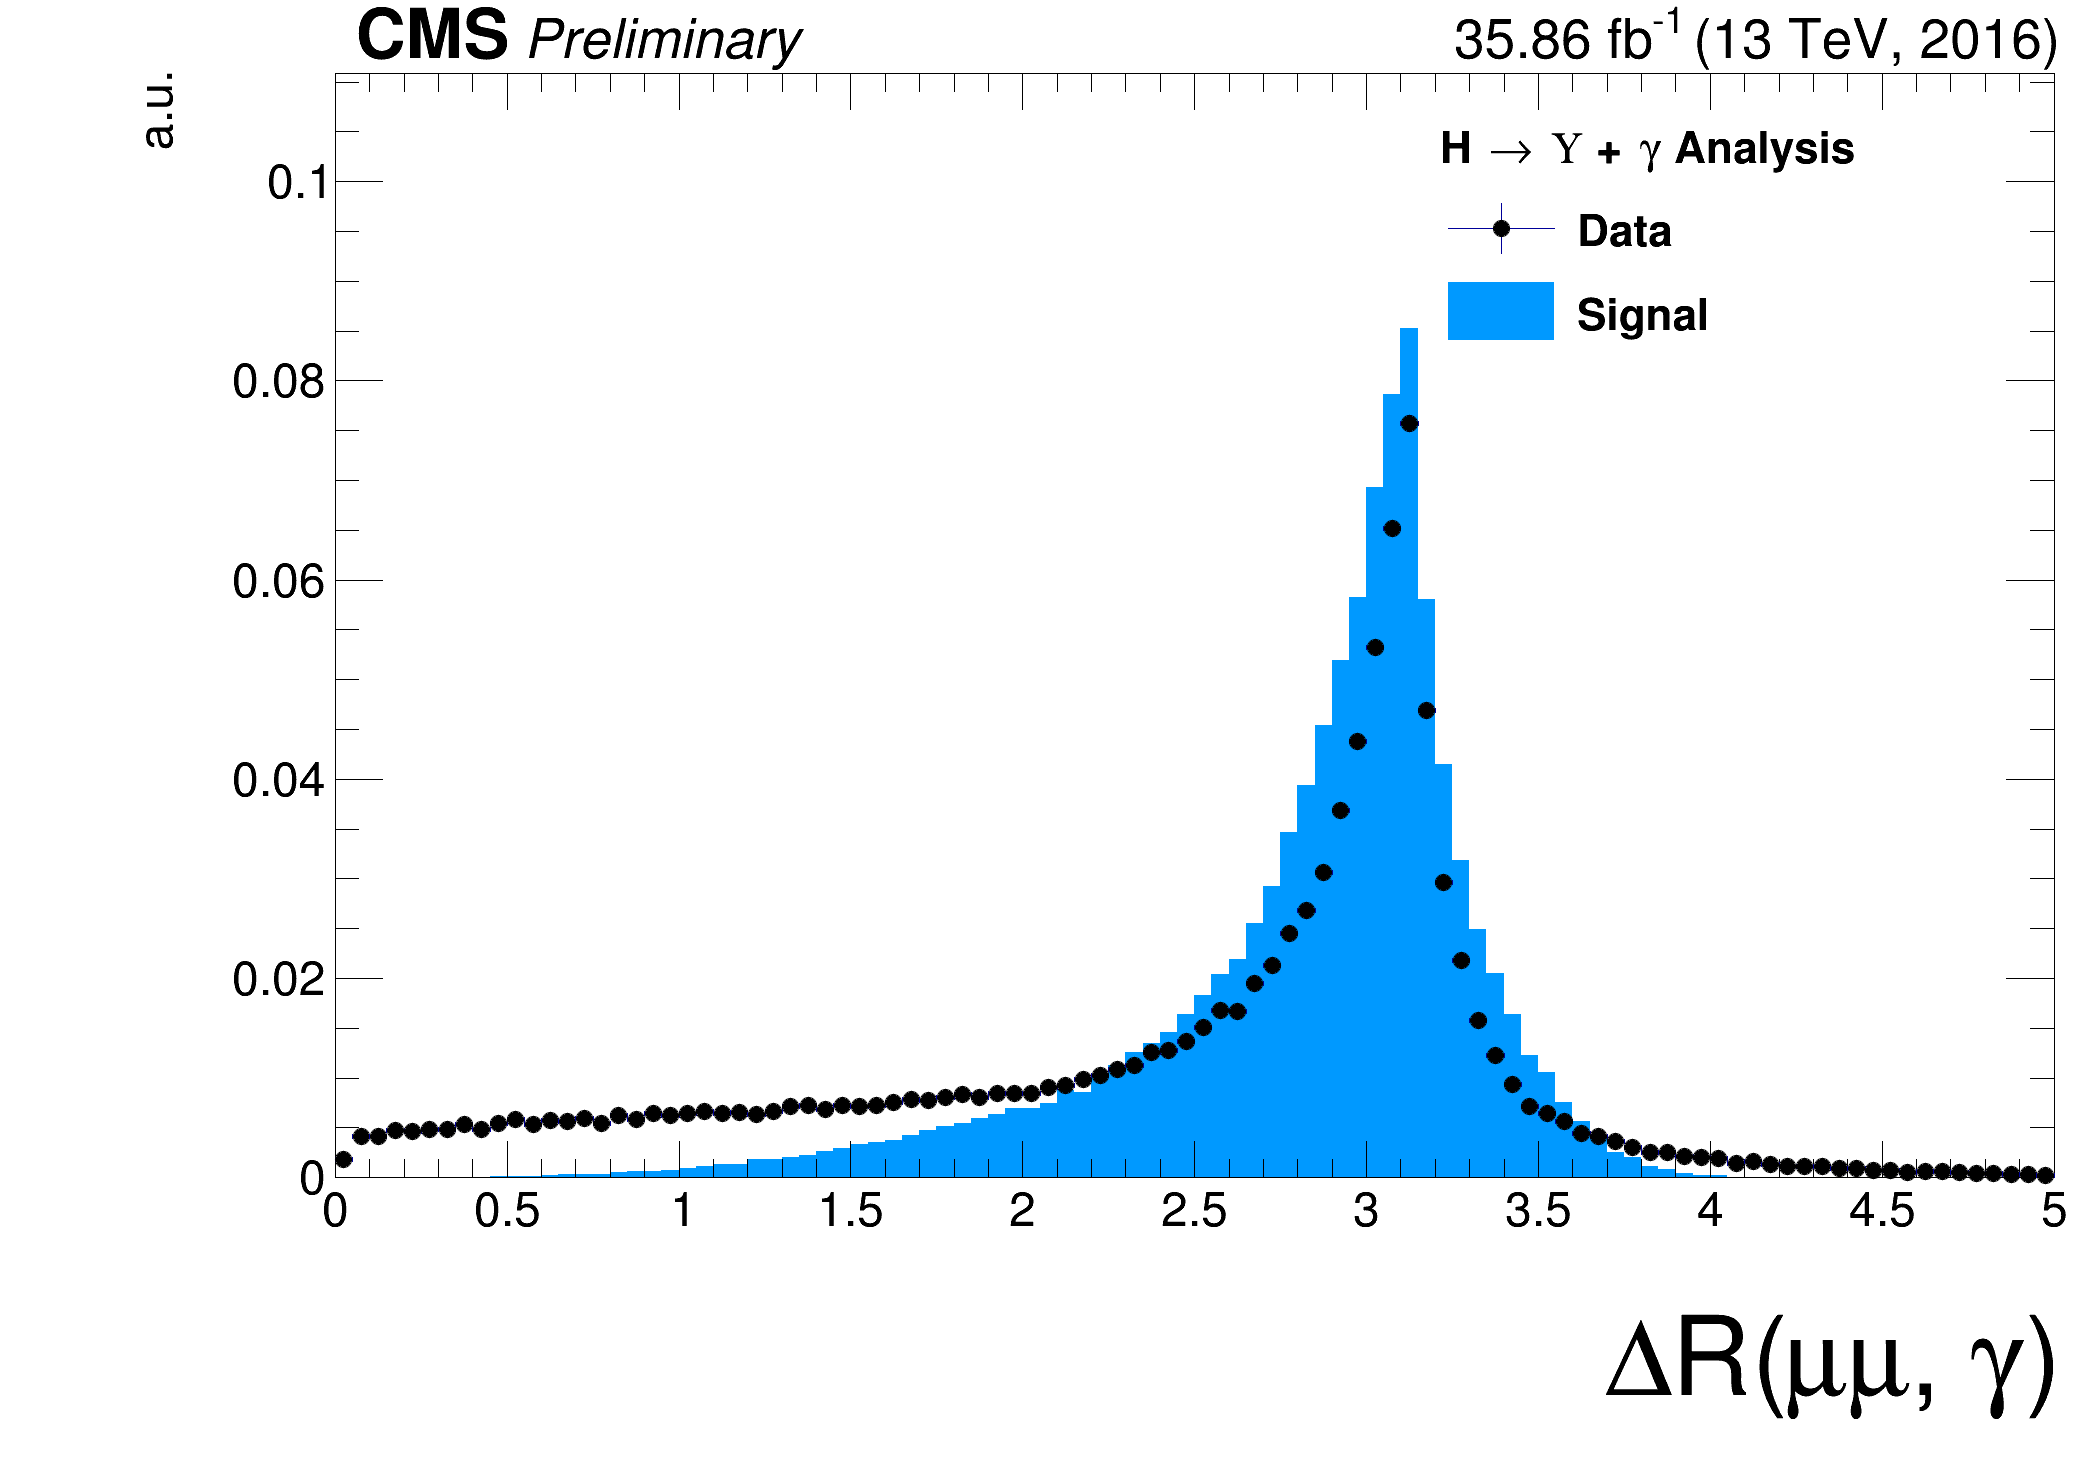
\includegraphics[width=0.45\textwidth]{figures_and_tables/outputPlots/HtoUpsilon_Cat0_ZZZZZ/au/data_x_mc/noKinCuts/h_noKin_deltaR_Upsilon_Photon}\hspace*{1.cm}
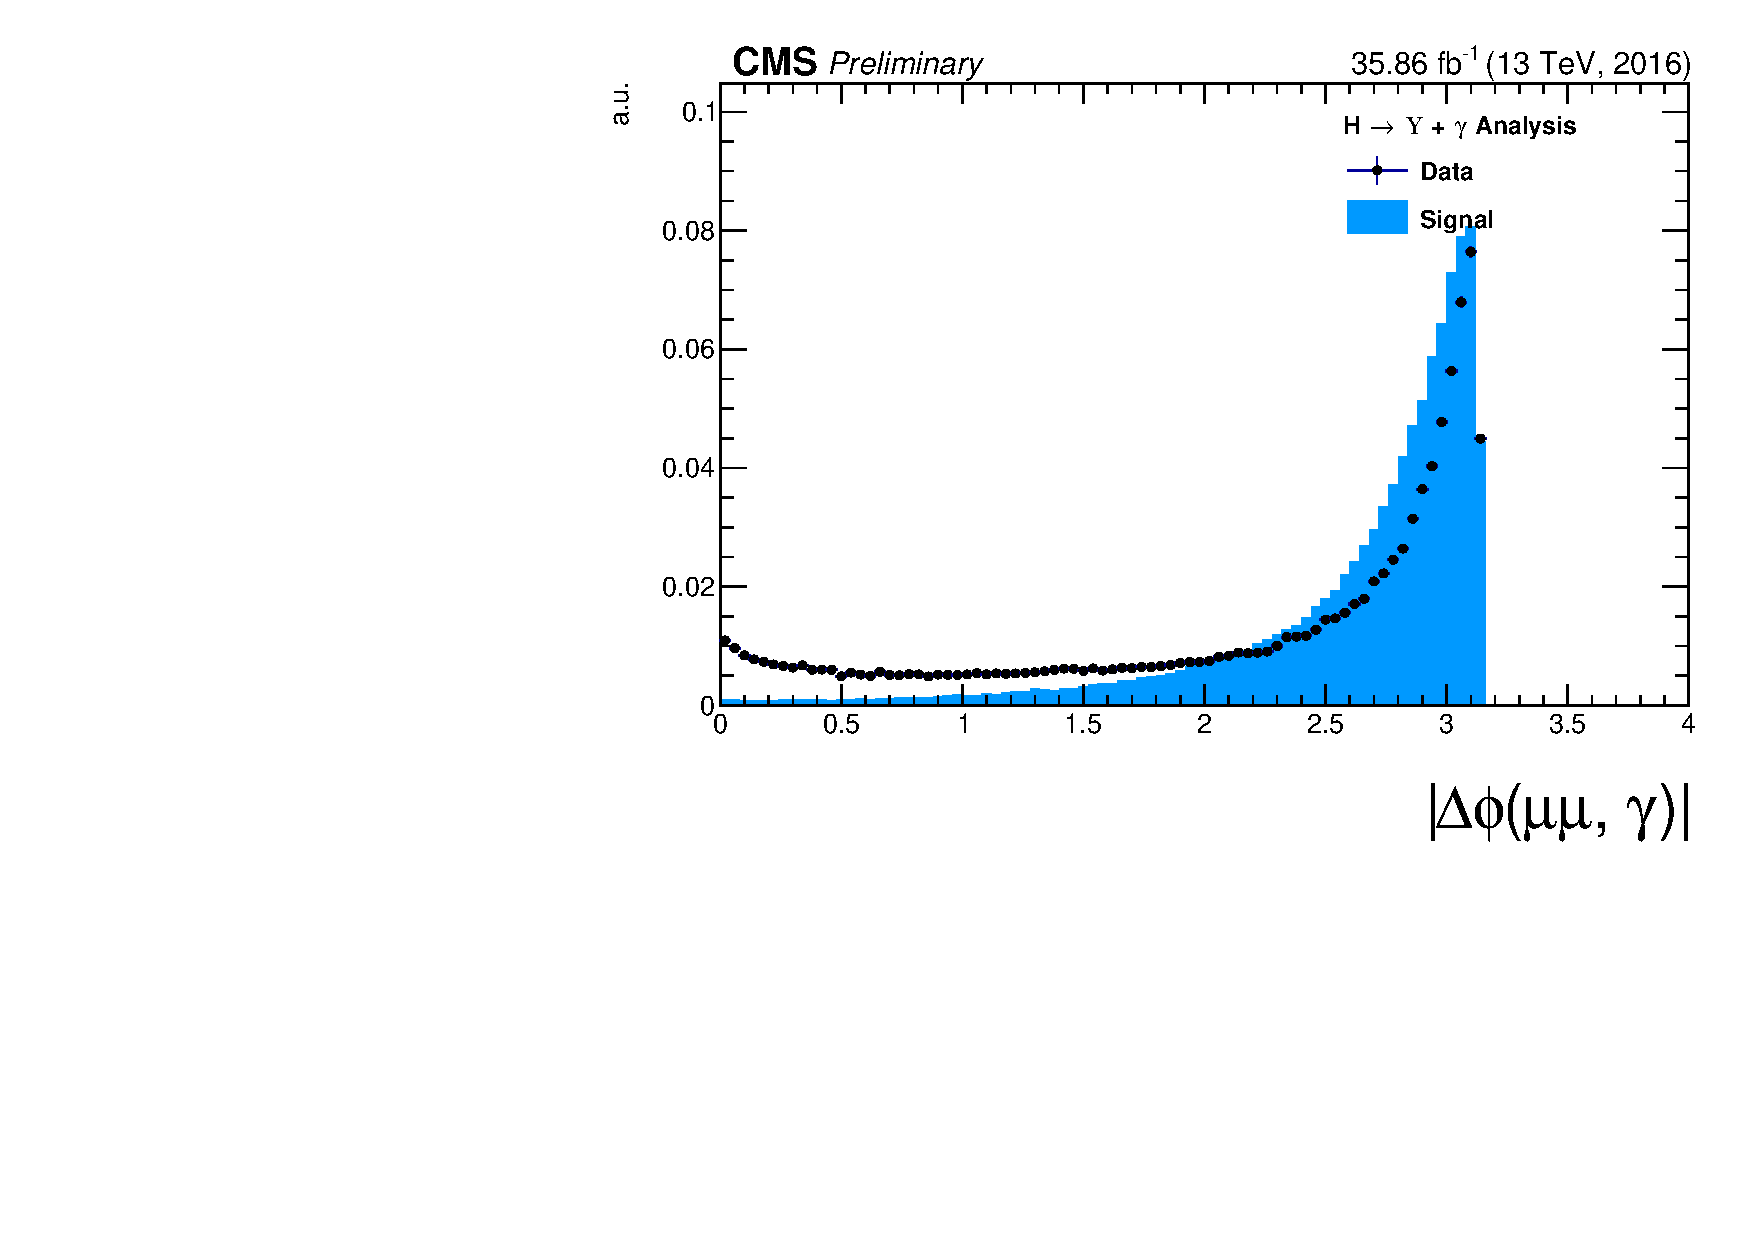
\includegraphics[width=0.45\textwidth]{figures_and_tables/outputPlots/HtoUpsilon_Cat0_ZZZZZ/au/data_x_mc/noKinCuts/h_noKin_deltaPhi_Upsilon_Photon}\end{center}\vspace*{-.5cm}
\caption{Left: The $\Delta R$ distributions between reconstructed dimuon ($\mu\mu$) system and the photon. Right: absolute value of the $\Delta \phi$ between the dimuon system and the photon for for Higgs decaying into $\Upsilon(1S,2S,3S)$ + $\gamma$ from data and signal events after Group I of selection cuts. The plots are normalized to the unit of area. The black dots are data collect by CMS while the blue distribution is related only to the signal Monte-Carlo generated samples.}
\label{fig:deltaRdeltaPhi_ZtoUpsilon_Cat0}
\end{figure}

%%%%%%% energy/mass ratio distributions for HtoUpsilon_Cat0
\begin{figure}[!htbp]
\begin{center}
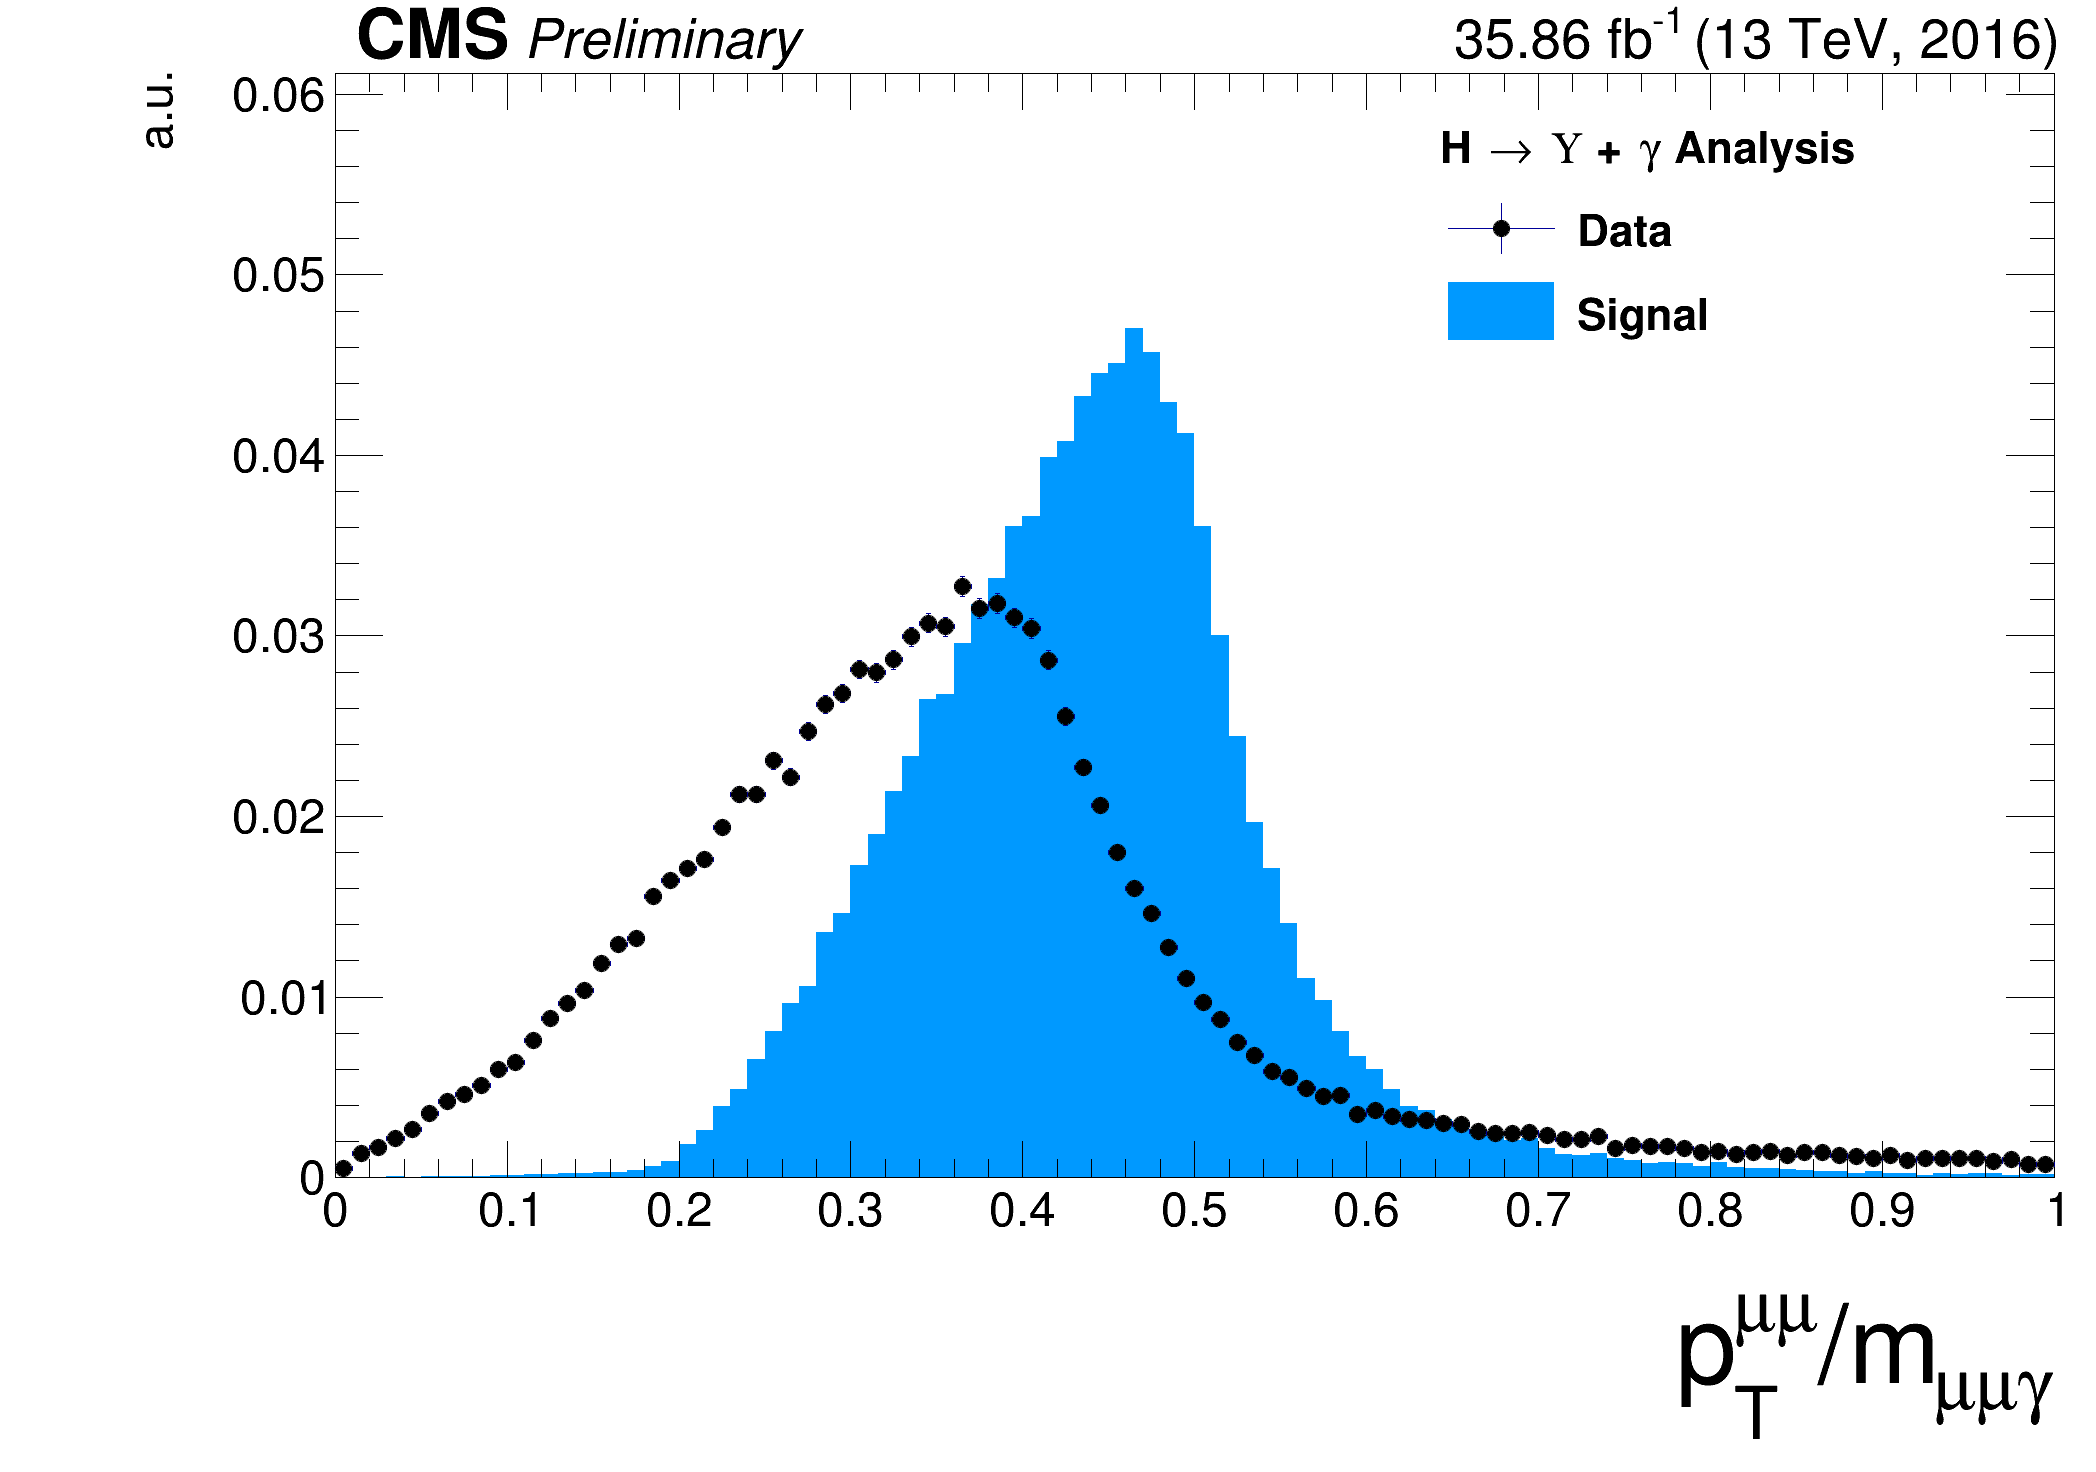
\includegraphics[width=0.45\textwidth]{figures_and_tables/outputPlots/HtoUpsilon_Cat0_ZZZZZ/au/data_x_mc/noKinCuts/h_noKin_upsilonPt_over_zMass}\hspace*{1.cm}
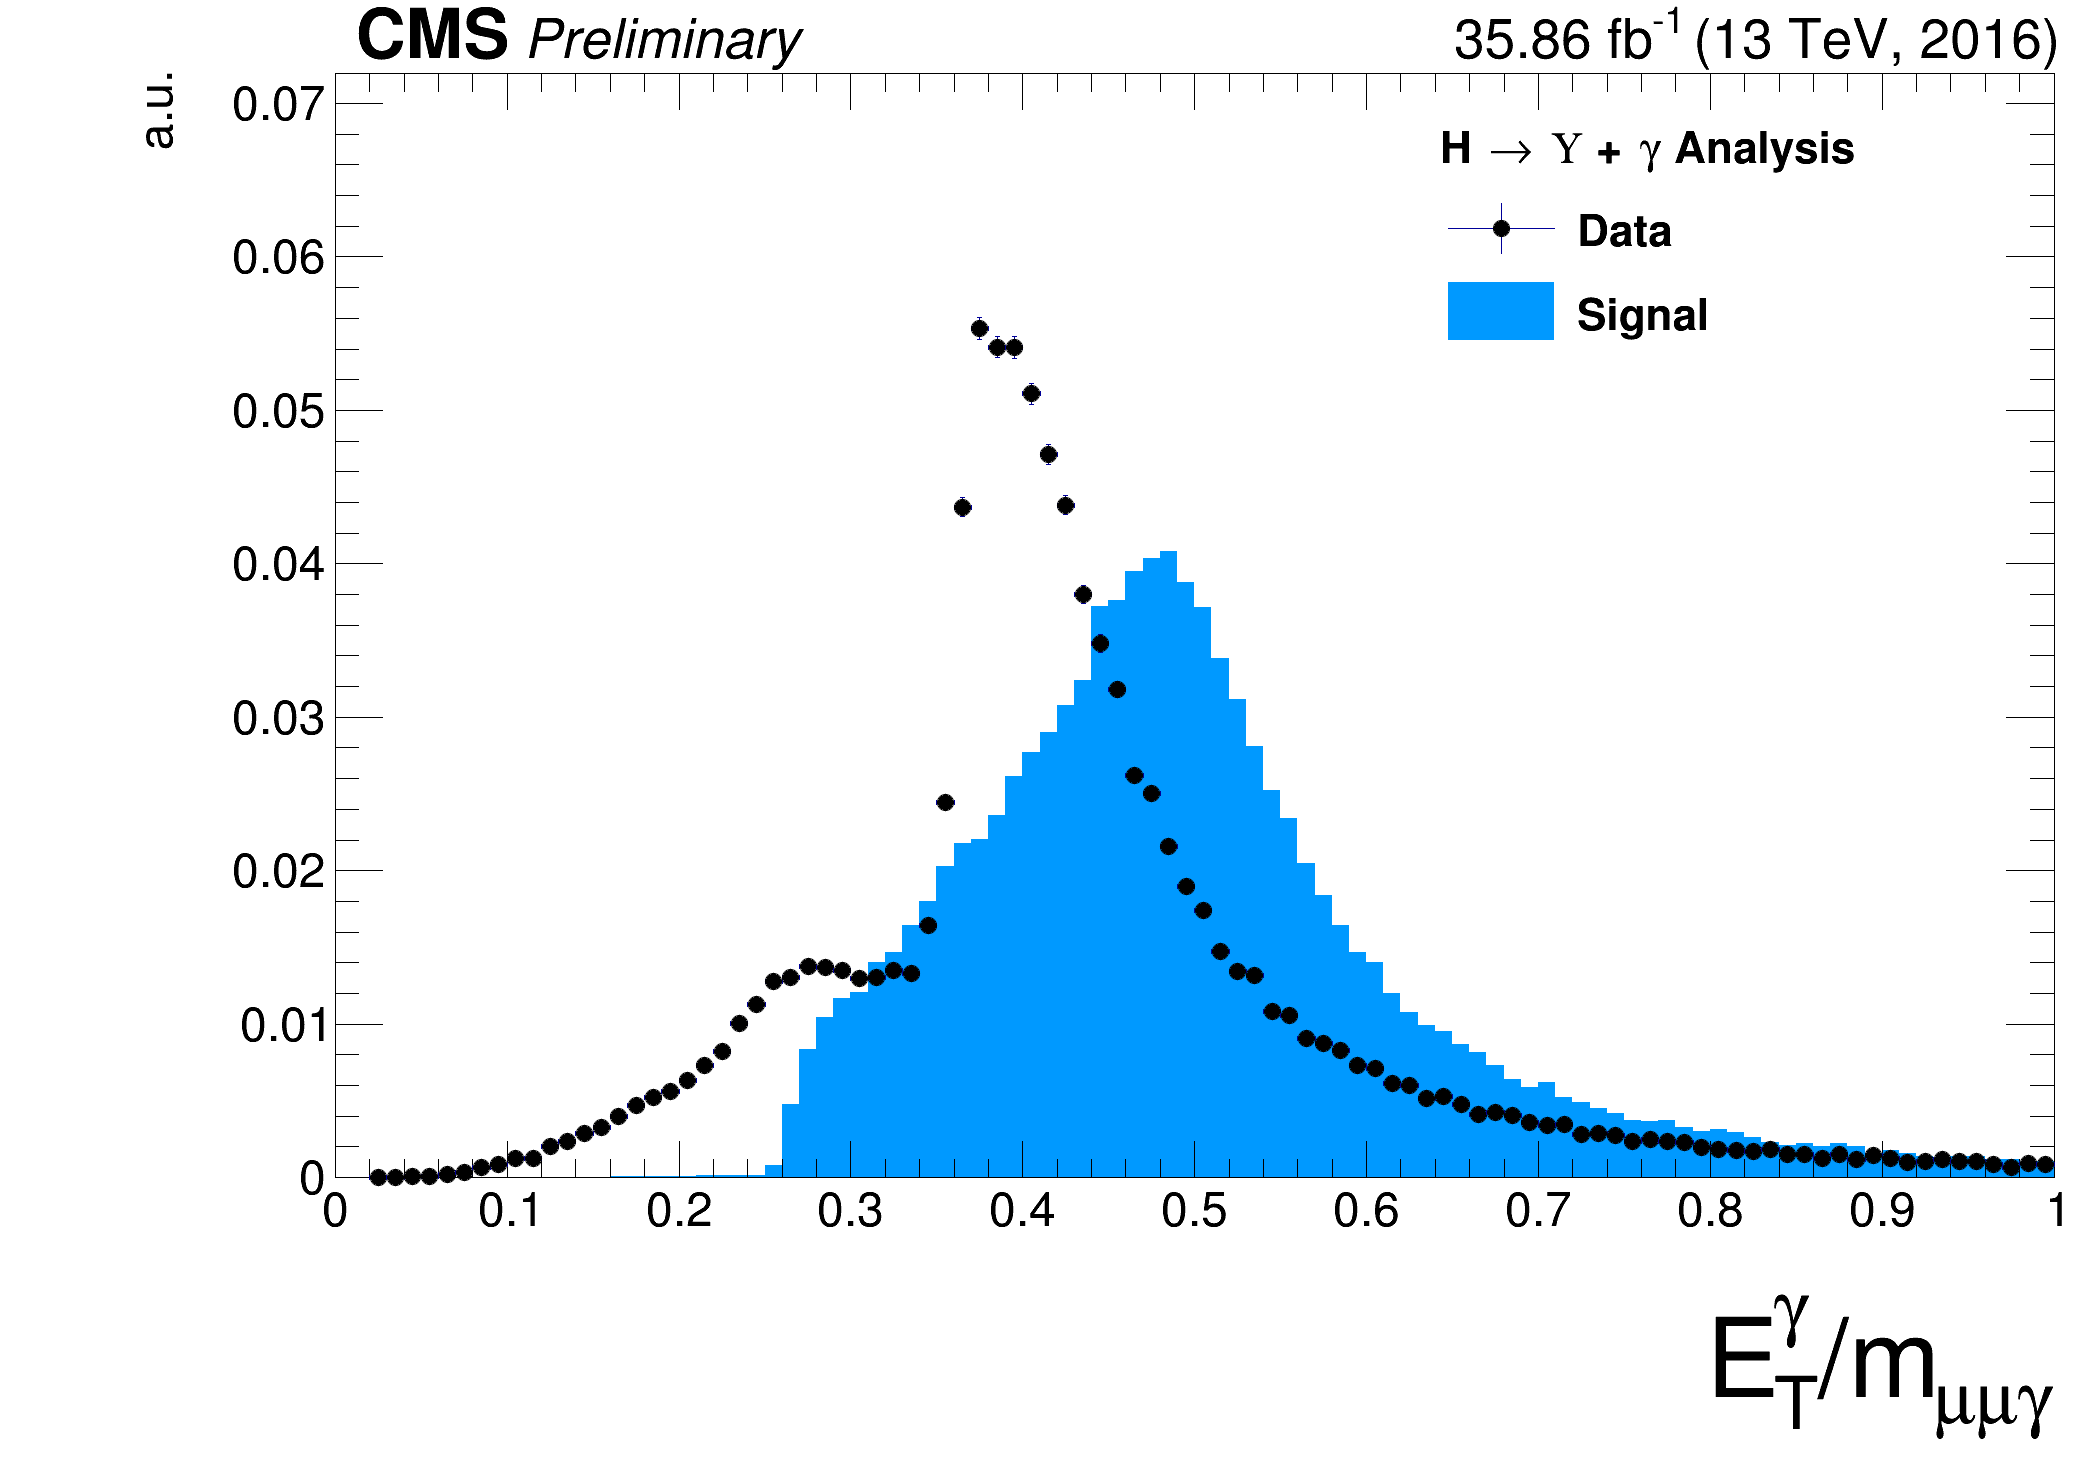
\includegraphics[width=0.45\textwidth]{figures_and_tables/outputPlots/HtoUpsilon_Cat0_ZZZZZ/au/data_x_mc/noKinCuts/h_noKin_photonPt_over_zMass}
\end{center}\vspace*{-.5cm}
\caption{The ratio for the transverse momentum of the reconstructed Upsilon and the reconstructed Higgs mass ($p_{T}^{\mu\mu}/M_{\mu\mu\gamma}$ - left) and the ratio for the transverse energy of the reconstructed Photon and the reconstructed Higgs mass ($E_{T}^{\gamma}/M_{\mu\mu\gamma}$ - right) distribution for Higgs decaying into $\Upsilon(1S,2S,3S)$ + $\gamma$ from data and signal events after Group I of selection cuts. The plots are normalized to the unit of area. The black dots are data collect by CMS while the blue distribution is related only to the signal Monte-Carlo generated samples.}
\label{fig:energy_ration_HtoUpsilon_Cat0}
\end{figure}

%%%%%%%%% dimuon mass distributions for HtoUpsilon_Cat0
\begin{figure}[!htbp]
\begin{center}
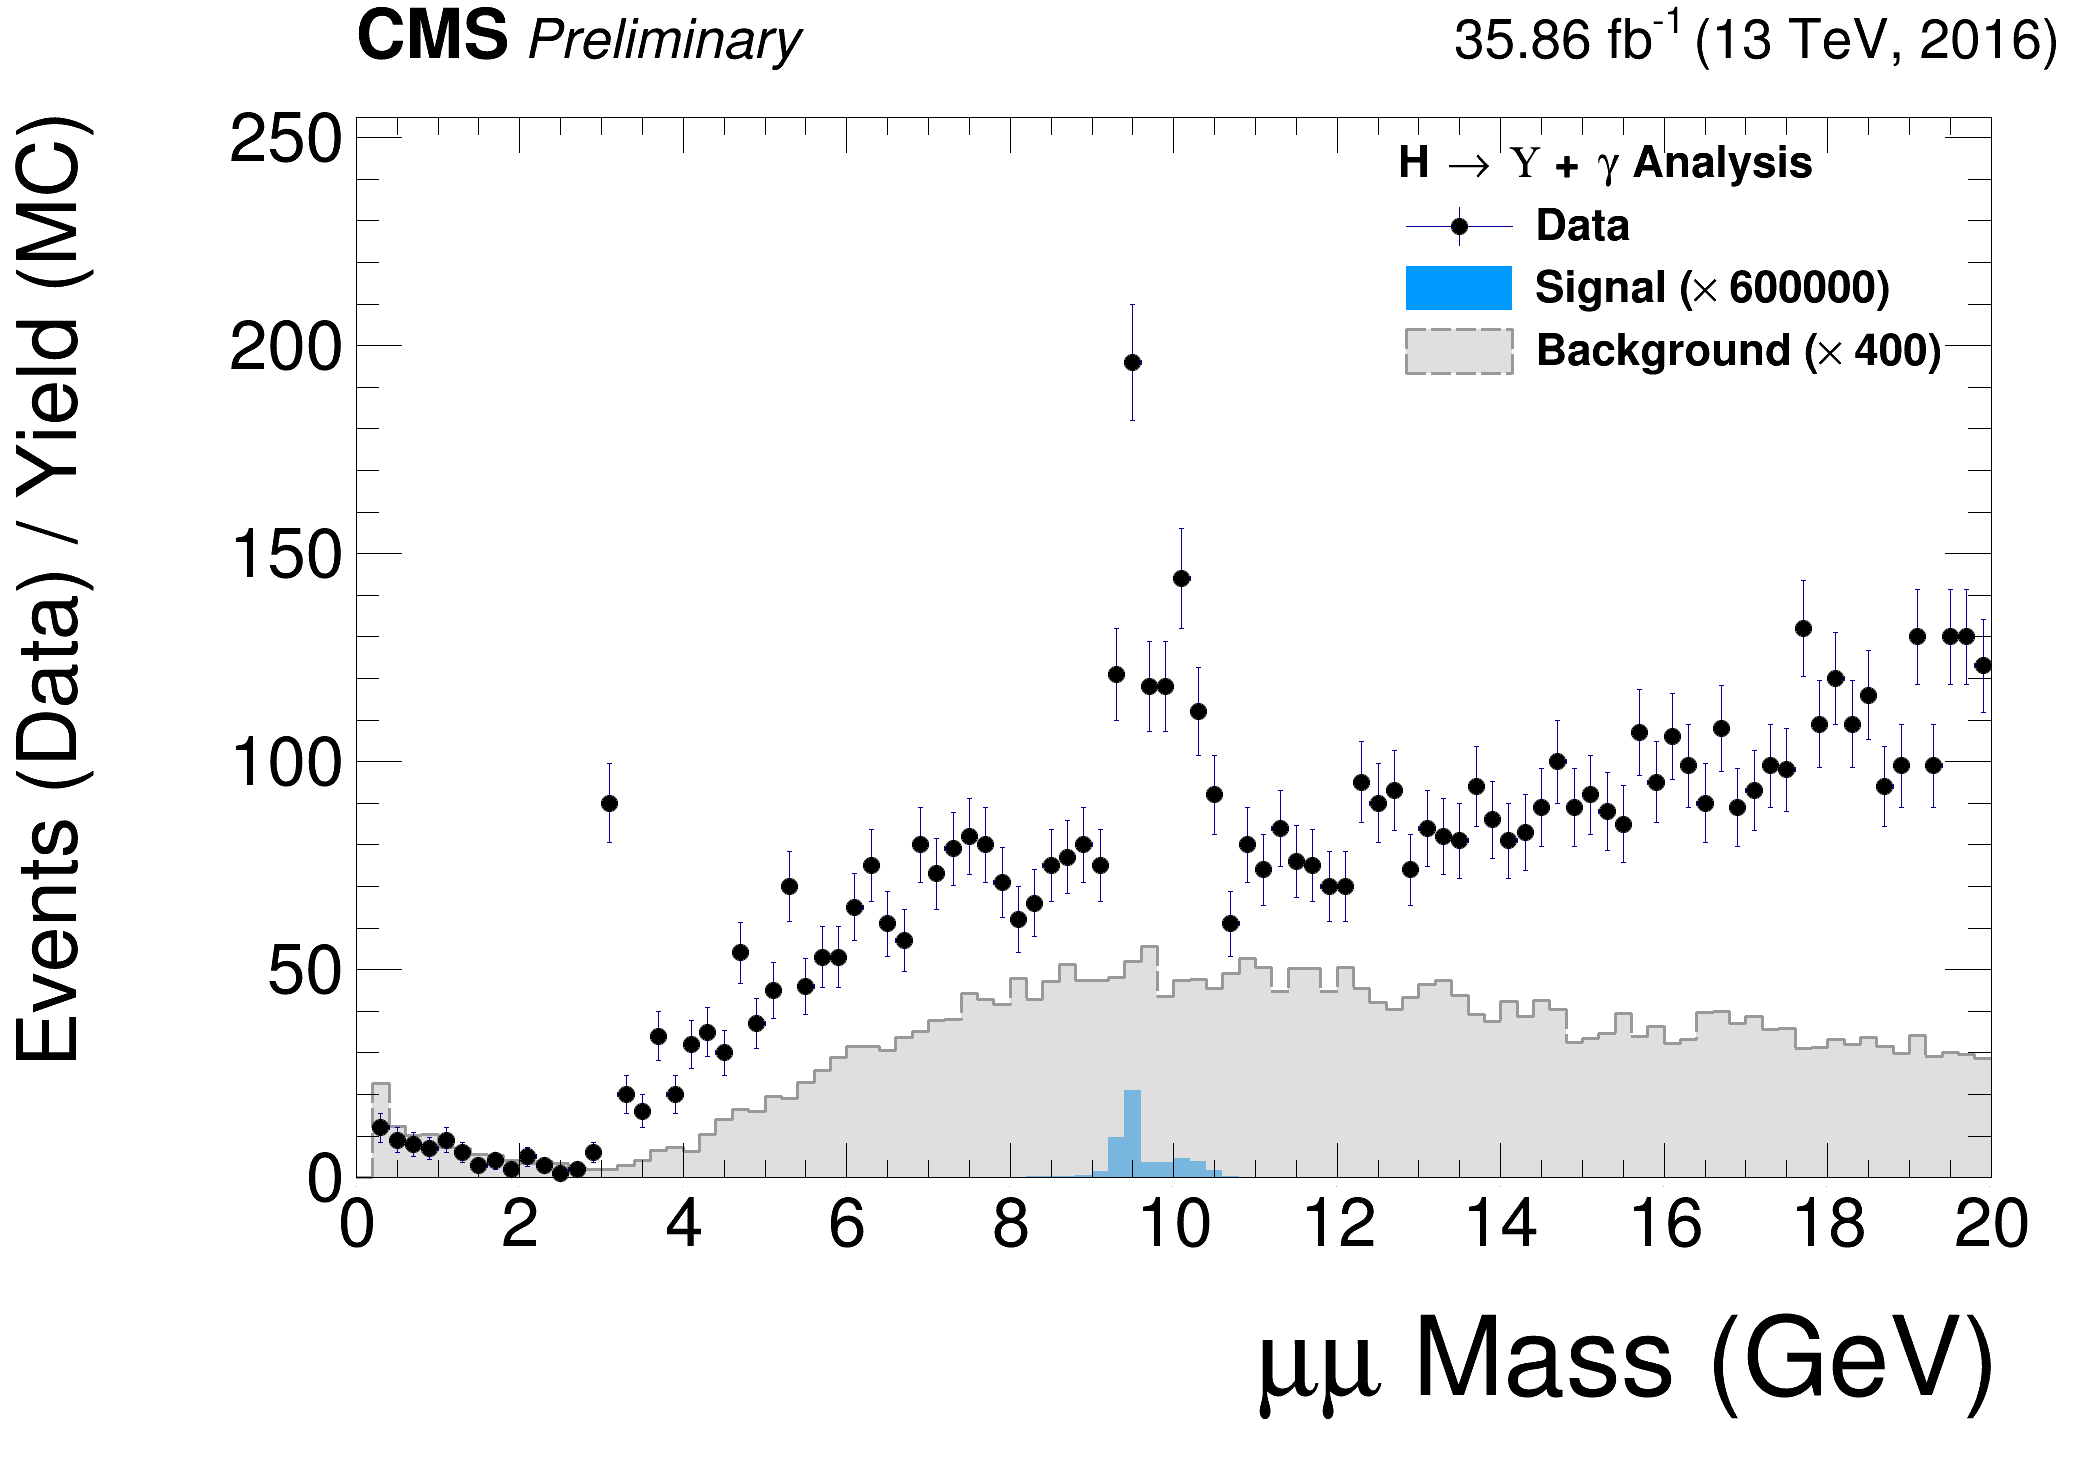
\includegraphics[width=0.45\textwidth]{figures_and_tables/outputPlots/HtoUpsilon_Cat0_ZZZZZ/nEvts/data_x_mc/noKinCuts/h_noKin_Upsilon_Mass_Signal_and_Background_LargeRange}\hspace*{1.cm}
\end{center}\vspace*{-.5cm}
\caption{The dimuon mass distribution of the reconstructed $\Upsilon (1S,2S,3S)$ from data and signal events for Higgs decaying after Group I of selection cuts. This plot is normalized the expected number of events.  "Signal" stands for the $H \rightarrow \Upsilon (1S,2S,3S) + \gamma$ sample (scaled by a factor of $\times 600000$) and "Background" corresponds to the resonant background (Higgs Dalitz Decay) sample (scaled by a factor of $\times 400$).}
\label{fig:dimuon_mass_HtoUpsilon_Cat0}
\end{figure}

%%%%%%%%%%%%%%%%%%%%%%%%%%%%%%%%%%%%%%%%%%%%%%%%%%%%%%%%%%%%%%%%%%%%%%%%%%%%%%%%%%%%%%%%%%%%%%%%%%%%%%%%%%%%%%%%%%%%%%%%
%%%%%%%%%%%%%%%%%%%%%%%%%%%%%%%%%%%%%%%%%%%%%%%%%%%%%%%%%%%%%%%%%%%%%%%%%%%%%%%%%%%%%%%%%%%%%%%%%%%%%%%%%%%%%%%%%%%%%%%%
%%%%%%%%%%%%%%%%%%%%%%%%%%%%%%%%%%%%%%%%%%%%%%%%%%%%%%%%%%%%%%%%%%%%%%%%%%%%%%%%%%%%%%%%%%%%%%%%%%%%%%%%%%%%%%%%%%%%%%%%
%%%%%%%%%%%%%%%%%%%%%%%%%%%%%%%%%%%%%%%%%%%%%%%%%%%%%%%%%%%%%%%%%%%%%%%%%%%%%%%%%%%%%%%%%%%%%%%%%%%%%%%%%%%%%%%%%%%%%%%%
%%%%%%%%%%%%%%%%%%%%%%%%%%%%%%%%%%%%%%%%%%%%%%%%%%%%%%%%%%%%%%%%%%%%%%%%%%%%%%%%%%%%%%%%%%%%%%%%%%%%%%%%%%%%%%%%%%%%%%%%
%%%%%%%%%%%%%%%%%%%%%%%%%%%%%%%%%%%%%%%%%%%%%%%%%%%%%%%%%%%%%%%%%%%%%%%%%%%%%%%%%%%%%%%%%%%%%%%%%%%%%%%%%%%%%%%%%%%%%%%%
%%%%%%%%%%%%%%%%%%%%%%%%%%%%%%%%%%%%%%%%%%%%%%%%%%%%%%%%%%%%%%%%%%%%%%%%%%%%%%%%%%%%%%%%%%%%%%%%%%%%%%%%%%%%%%%%%%%%%%%%
%%%%%%%%%%%%%%%%%%%%%%%%%%%%%%%%%%%%%%%%%%%%%%%%%%%%%%%%%%%%%%%%%%%%%%%%%%%%%%%%%%%%%%%%%%%%%%%%%%%%%%%%%%%%%%%%%%%%%%%%
%%%%%%%%%%%%%%%%%%%%%%%%%%%%%%%%%%%%%%%%%%%%%%%%%%%%%%%%%%%%%%%%%%%%%%%%%%%%%%%%%%%%%%%%%%%%%%%%%%%%%%%%%%%%%%%%%%%%%%%%
%%%%%%%%%%%%%%%%%%%%%%%%%%%%%%%%%%%%%%%%%%%%%%%%%%%%%%%%%%%%%%%%%%%%%%%%%%%%%%%%%%%%%%%%%%%%%%%%%%%%%%%%%%%%%%%%%%%%%%%%
%%%%%%%%%%%%%%%%%%%%%%%%%%%%%%%%%%%%%%%%%%%%%%%%%%%%%%%%%%%%%%%%%%%%%%%%%%%%%%%%%%%%%%%%%%%%%%%%%%%%%%%%%%%%%%%%%%%%%%%%
%%%%%%%%%%%%%%%%%%%%%%%%%%%%%%%%%%%%%%%%%%%%%%%%%%%%%%%%%%%%%%%%%%%%%%%%%%%%%%%%%%%%%%%%%%%%%%%%%%%%%%%%%%%%%%%%%%%%%%%%
%%%%%%%%%%%%%%%%%%%%%%%%%%%%%%%%%%%%%%%%%%%%%%%%%%%%%%%%%%%%%%%%%%%%%%%%%%%%%%%%%%%%%%%%%%%%%%%%%%%%%%%%%%%%%%%%%%%%%%%%
%
%
% _______  ______    _______  __   __  _______    ___   ___  
%|       ||    _ |  |       ||  | |  ||       |  |   | |   | 
%|    ___||   | ||  |   _   ||  | |  ||    _  |  |   | |   | 
%|   | __ |   |_||_ |  | |  ||  |_|  ||   |_| |  |   | |   | 
%|   ||  ||    __  ||  |_|  ||       ||    ___|  |   | |   | 
%|   |_| ||   |  | ||       ||       ||   |      |   | |   | 
%|_______||___|  |_||_______||_______||___|      |___| |___| 
%
%%%%%%%%%%%%%%%%%%%%%%%%%%%%%%%%%%%%%%%%%%%%%%%%%%%%%%%%%%%%%%%%%%%%%%%%%%%%%%%%%%%%%%%%%%%%%%%%%%%%%%%%%%%%%%%%%%%%%%%%
%%%%%%%%%%%%%%%%%%%%%%%%%%%%%%%%%%%%%%%%%%%%%%%%%%%%%%%%%%%%%%%%%%%%%%%%%%%%%%%%%%%%%%%%%%%%%%%%%%%%%%%%%%%%%%%%%%%%%%%%
%%%%%%%%%%%%%%%%%%%%%%%%%%%%%%%%%%%%%%%%%%%%%%%%%%%%%%%%%%%%%%%%%%%%%%%%%%%%%%%%%%%%%%%%%%%%%%%%%%%%%%%%%%%%%%%%%%%%%%%%
%%%%%%%%%%%%%%%%%%%%%%%%%%%%%%%%%%%%%%%%%%%%%%%%%%%%%%%%%%%%%%%%%%%%%%%%%%%%%%%%%%%%%%%%%%%%%%%%%%%%%%%%%%%%%%%%%%%%%%%%
%%%%%%%%%%%%%%%%%%%%%%%%%%%%%%%%%%%%%%%%%%%%%%%%%%%%%%%%%%%%%%%%%%%%%%%%%%%%%%%%%%%%%%%%%%%%%%%%%%%%%%%%%%%%%%%%%%%%%%%%
%%%%%%%%%%%%%%%%%%%%%%%%%%%%%%%%%%%%%%%%%%%%%%%%%%%%%%%%%%%%%%%%%%%%%%%%%%%%%%%%%%%%%%%%%%%%%%%%%%%%%%%%%%%%%%%%%%%%%%%%
%%%%%%%%%%%%%%%%%%%%%%%%%%%%%%%%%%%%%%%%%%%%%%%%%%%%%%%%%%%%%%%%%%%%%%%%%%%%%%%%%%%%%%%%%%%%%%%%%%%%%%%%%%%%%%%%%%%%%%%%
%%%%%%%%%%%%%%%%%%%%%%%%%%%%%%%%%%%%%%%%%%%%%%%%%%%%%%%%%%%%%%%%%%%%%%%%%%%%%%%%%%%%%%%%%%%%%%%%%%%%%%%%%%%%%%%%%%%%%%%%
%%%%%%%%%%%%%%%%%%%%%%%%%%%%%%%%%%%%%%%%%%%%%%%%%%%%%%%%%%%%%%%%%%%%%%%%%%%%%%%%%%%%%%%%%%%%%%%%%%%%%%%%%%%%%%%%%%%%%%%%
%%%%%%%%%%%%%%%%%%%%%%%%%%%%%%%%%%%%%%%%%%%%%%%%%%%%%%%%%%%%%%%%%%%%%%%%%%%%%%%%%%%%%%%%%%%%%%%%%%%%%%%%%%%%%%%%%%%%%%%%
%%%%%%%%%%%%%%%%%%%%%%%%%%%%%%%%%%%%%%%%%%%%%%%%%%%%%%%%%%%%%%%%%%%%%%%%%%%%%%%%%%%%%%%%%%%%%%%%%%%%%%%%%%%%%%%%%%%%%%%%
%%%%%%%%%%%%%%%%%%%%%%%%%%%%%%%%%%%%%%%%%%%%%%%%%%%%%%%%%%%%%%%%%%%%%%%%%%%%%%%%%%%%%%%%%%%%%%%%%%%%%%%%%%%%%%%%%%%%%%%%
%%%%%%%%%%%%%%%%%%%%%%%%%%%%%%%%%%%%%%%%%%%%%%%%%%%%%%%%%%%%%%%%%%%%%%%%%%%%%%%%%%%%%%%%%%%%%%%%%%%%%%%%%%%%%%%%%%%%%%%%
%%%%%%%%%%%%%%%%%%%%%%%%%%%%%%%%%%%%%%%%%%%%%%%%%%%%%%%%%%%%%%%%%%%%%%%%%%%%%%%%%%%%%%%%%%%%%%%%%%%%%%%%%%%%%%%%%%%%%%%%
%%%%%%%%%%%%%%%%%%%%%%%%%%%%%%%%%%%%%%%%%%%%%%%%%%%%%%%%%%%%%%%%%%%%%%%%%%%%%%%%%%%%%%%%%%%%%%%%%%%%%%%%%%%%%%%%%%%%%%%%

\clearpage

\section{Kinematical selection (Group II)}


After all Trigger and Object Identification cuts, described in before (\textbf{Group I}), a set of kinematical cuts are applied in order to improve the signal to background relation. They are

\begin{itemize}
  \item $\Delta R(\text{leading }\mu, \gamma) > 1$;
  \item $\Delta R(\text{trailing }\mu, \gamma) > 1$;
  \item $\Delta R(\mu\mu, \gamma) > 2$;
  \item $|\Delta \phi (\text{leading }\mu, \gamma)| > 1.5$;
  \item 8.4 GeV $<$ $M_{\mu\mu}$ $<$ 11.1 GeV;
  \item $E_{T}^{\gamma}/M_{\mu\mu\gamma} > 35/91.2 \text{ for the Z decay or } 35/125 \text{ for the Higgs decay} $;
  \item $p_{T}^{\mu\mu}/M_{\mu\mu\gamma} > 35/91.2 \text{ for the Z decay or } 35/125 \text{ for the Higgs decay} $.
\end{itemize}

The choice of these thresholds were based on the visual inspection of the distributions (besides the invariant mass distribution of the dimuon system $M_{\mu\mu}$, which needs to be defined around the $\Upsilon(1S, 2S, 3S)$ mass) and to keep this analysis in phase with other similar analysis within CMS.

% A detailed discussion about the choices on the thresholds can be found in the $H/Z \rightarrow J/\psi + \gamma$ analysis \cite{CMS_jpsi_analysis}. In any case, besides the dimuon mass window, which obviously should match with the $\Upsilon(1S,2S,3S)$ mass, the values were not changed, with respect to the reference analysis. Even though some optimization was tried, it brought no reasonable gain that would justify change the thresholds and lose compatibility with the $J/\psi$ study.

Below it is shown the same set of plot shown before, but this time, taking into account the full selection (\textbf{Group I+II}).


%CONTROL PLOTS
%%$\pT$ muon distributions for ZtoUpsilon_Cat0
\begin{figure}[!htbp]
\begin{center}
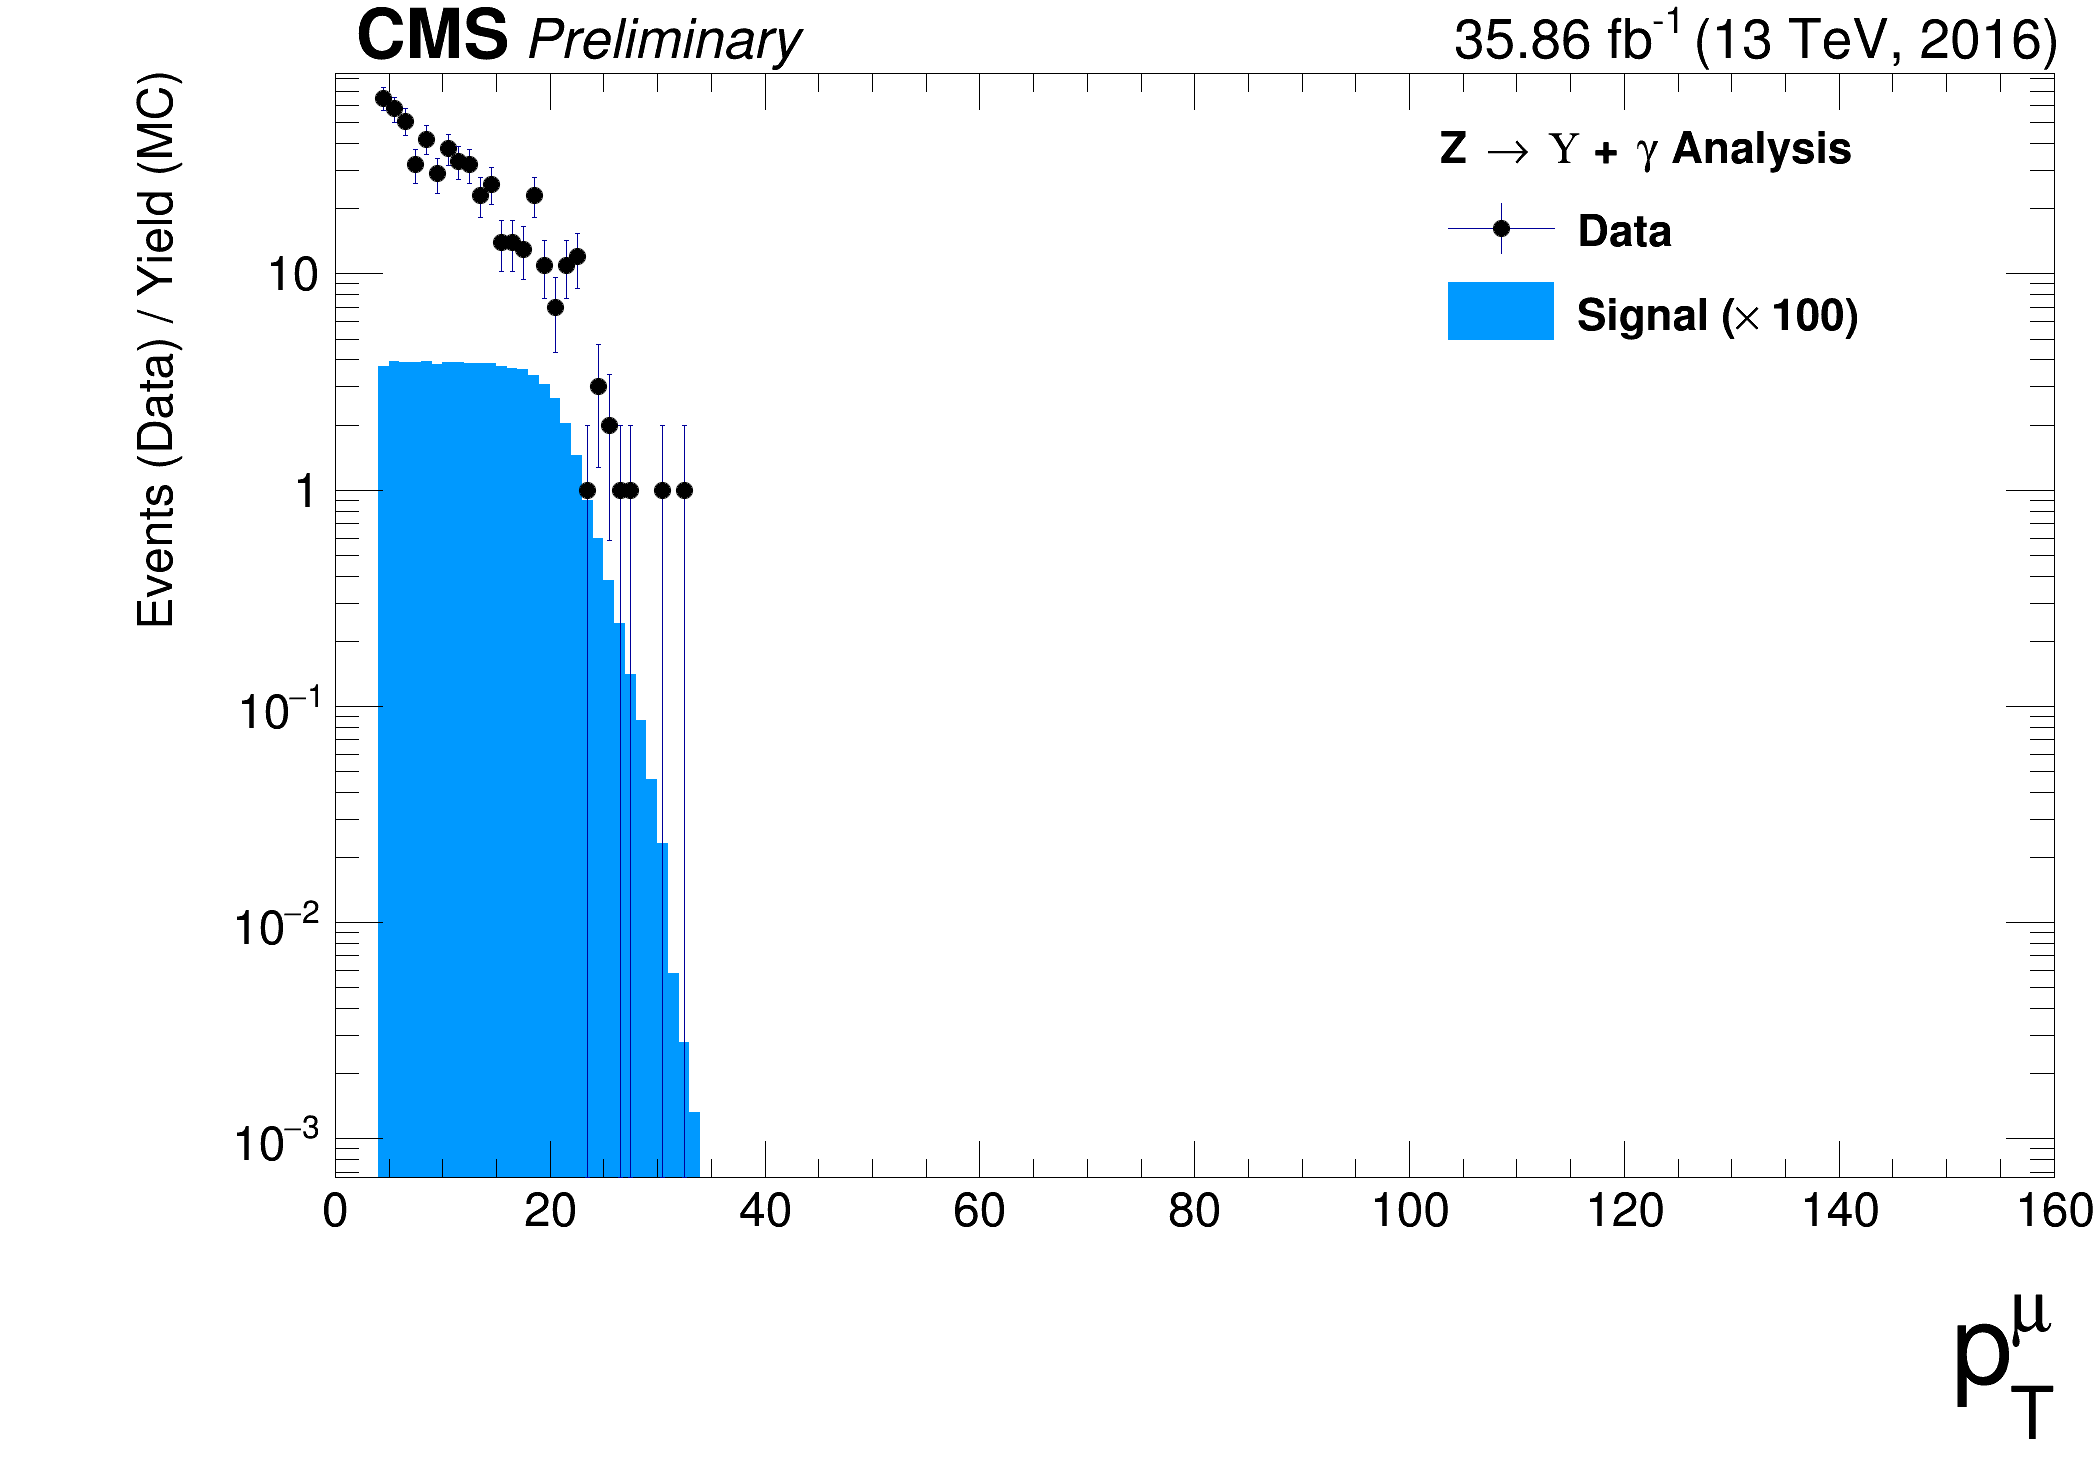
\includegraphics[width=0.45\textwidth]{figures_and_tables/outputPlots/ZtoUpsilon_Cat0_ZZZZZ/nEvts/data_x_mc/withKinCuts/h_withKin_TrailingMu_pt}\hspace*{1.cm}
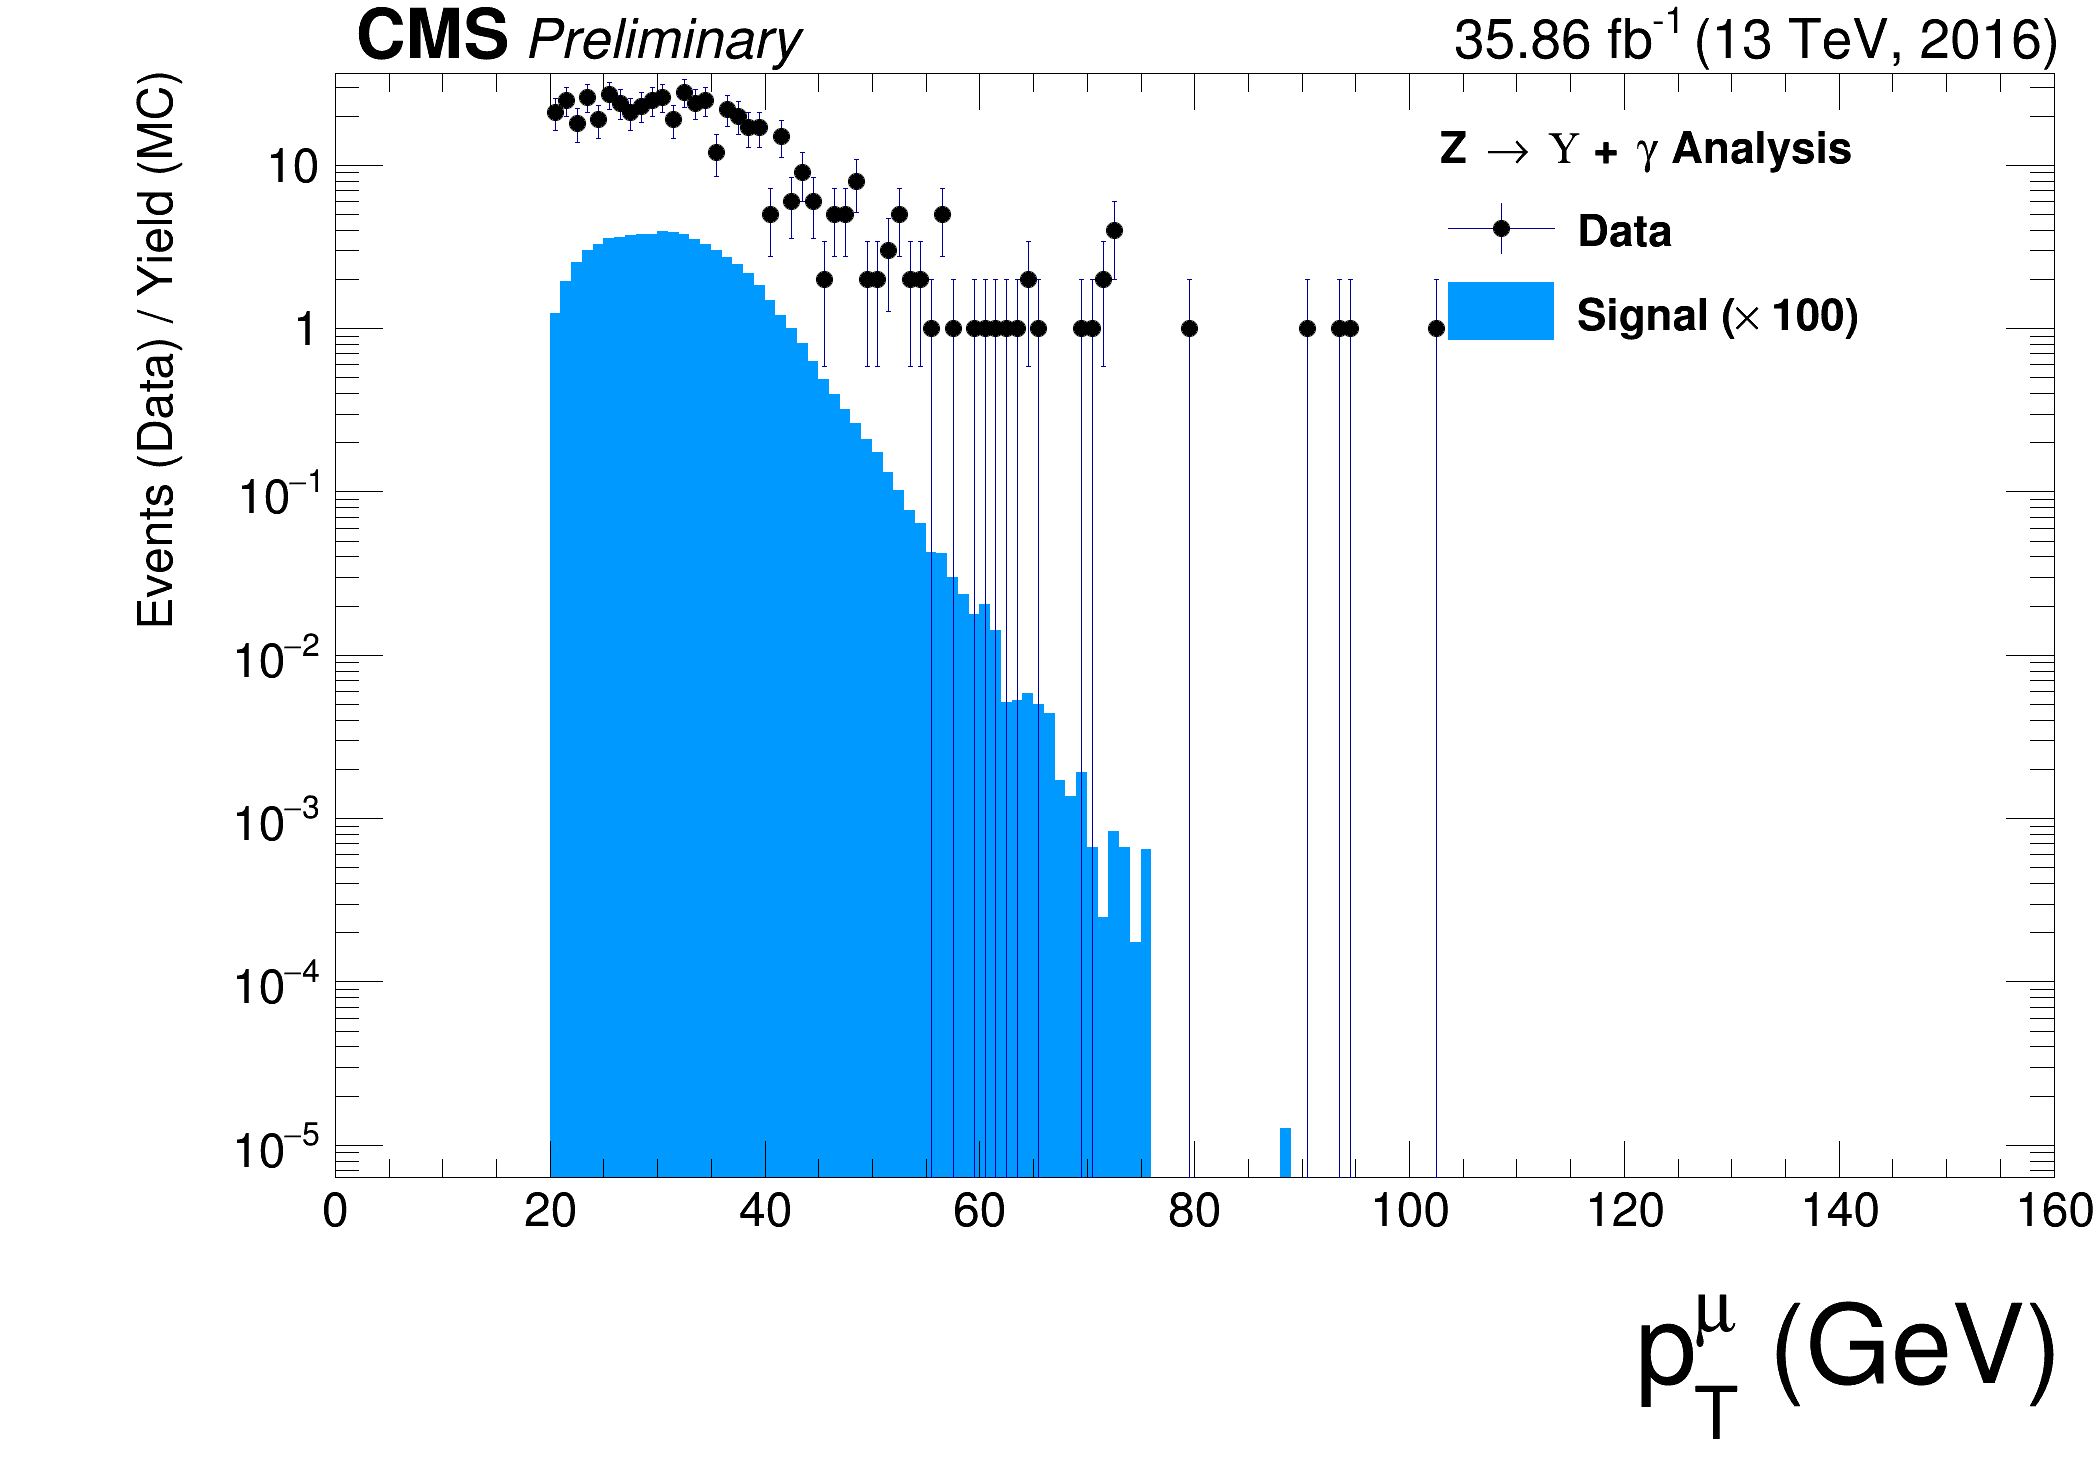
\includegraphics[width=0.45\textwidth]{figures_and_tables/outputPlots/ZtoUpsilon_Cat0_ZZZZZ/nEvts/data_x_mc/withKinCuts/h_withKin_LeadingMu_pt}
\end{center}\vspace*{-.5cm}
\caption{The \PT muon distributions from data and signal events for Z decaying into $\Upsilon(1S,2S,3S)$ + $\gamma$ after Group I+II of selection cuts, where on left are presenting the trailing muons and on right are the leading muons. The plots are normalized to the number of events. Signal sample is scaled by a factor of $\times 100$). The black dots are data collect by CMS while the blue distribution is related only to the signal Monte-Carlo generated samples.}
\label{fig:pTMuons_ZtoUpsilon_Cat0_groupI_plus_II}
\end{figure}


%%%%%%%$\eta$ muon distributions for ZtoUpsilon_Cat0
\begin{figure}[!htbp]
\begin{center}
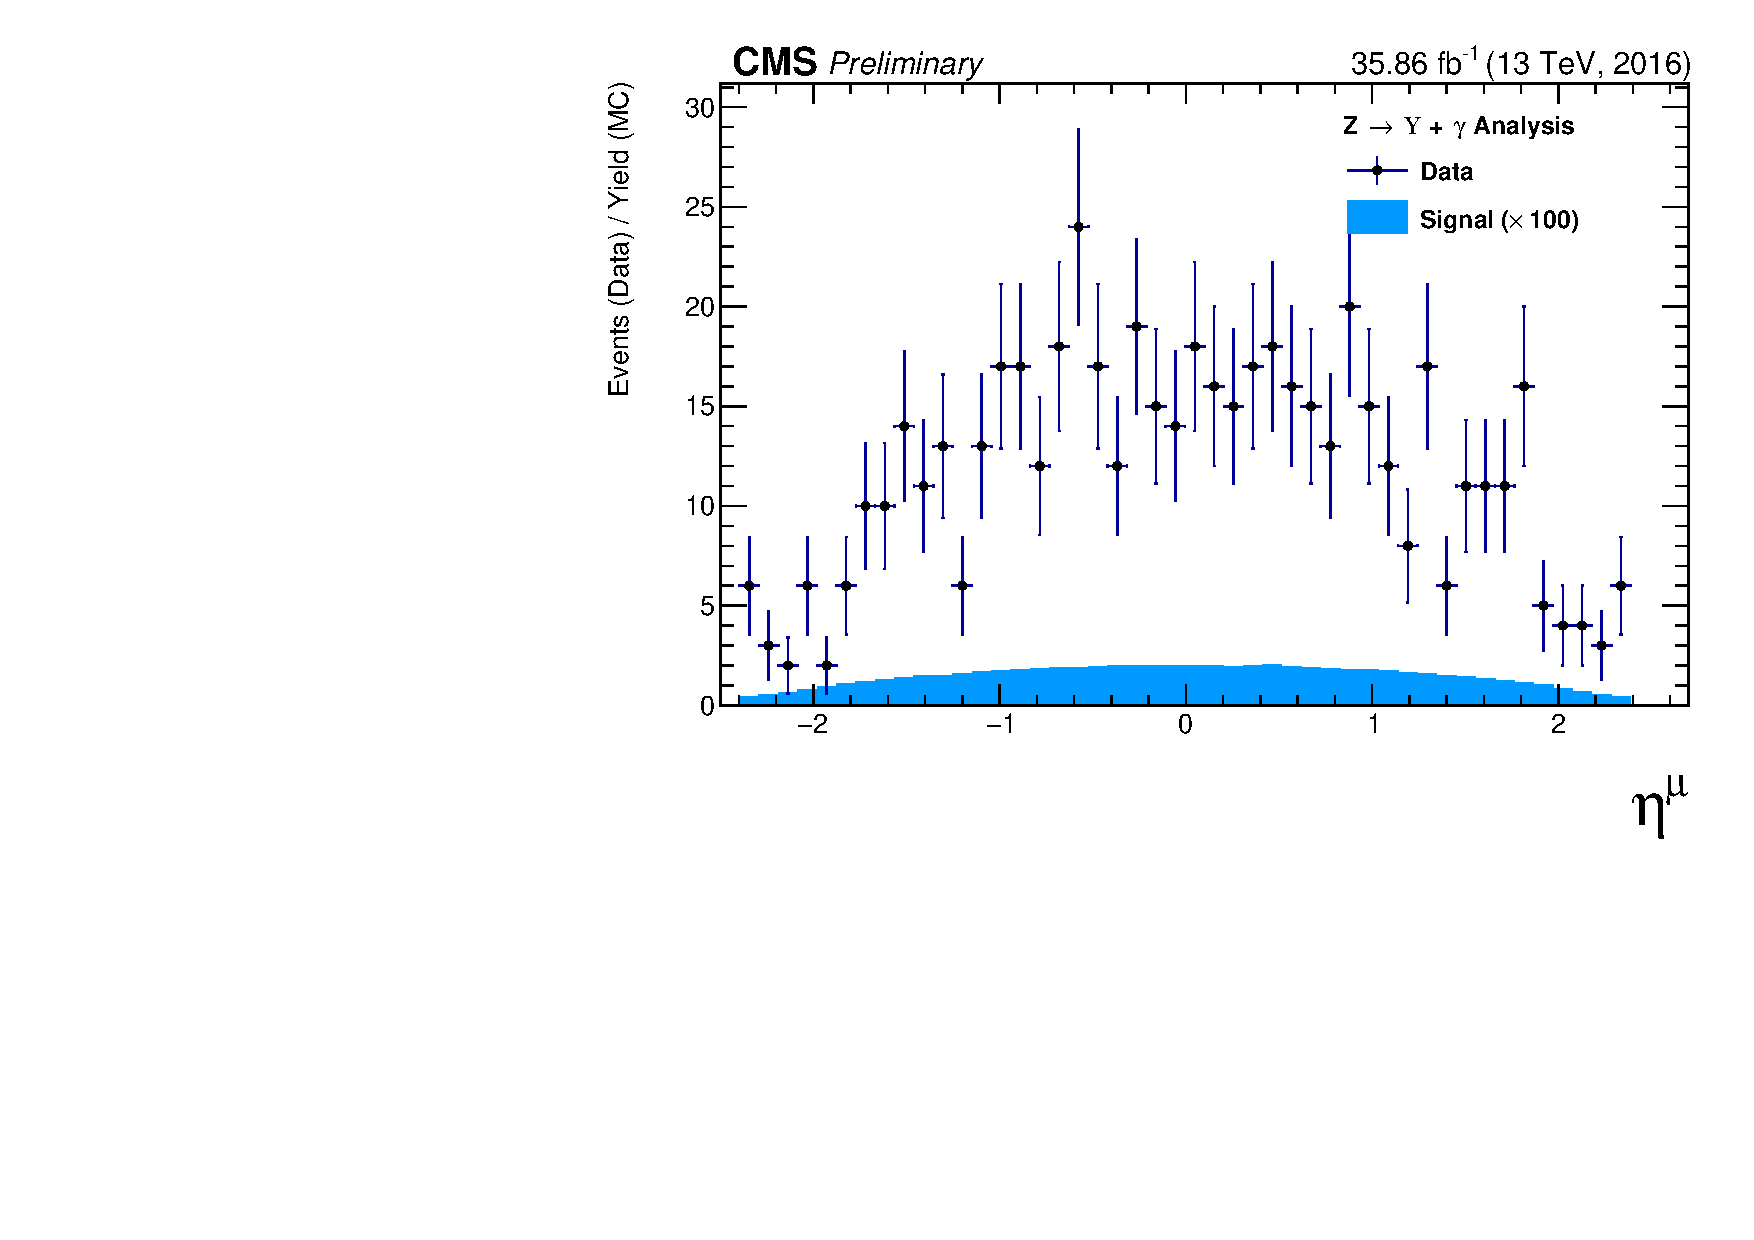
\includegraphics[width=0.45\textwidth]{figures_and_tables/outputPlots/ZtoUpsilon_Cat0_ZZZZZ/nEvts/data_x_mc/withKinCuts/h_withKin_TrailingMu_eta}\hspace*{1.cm}
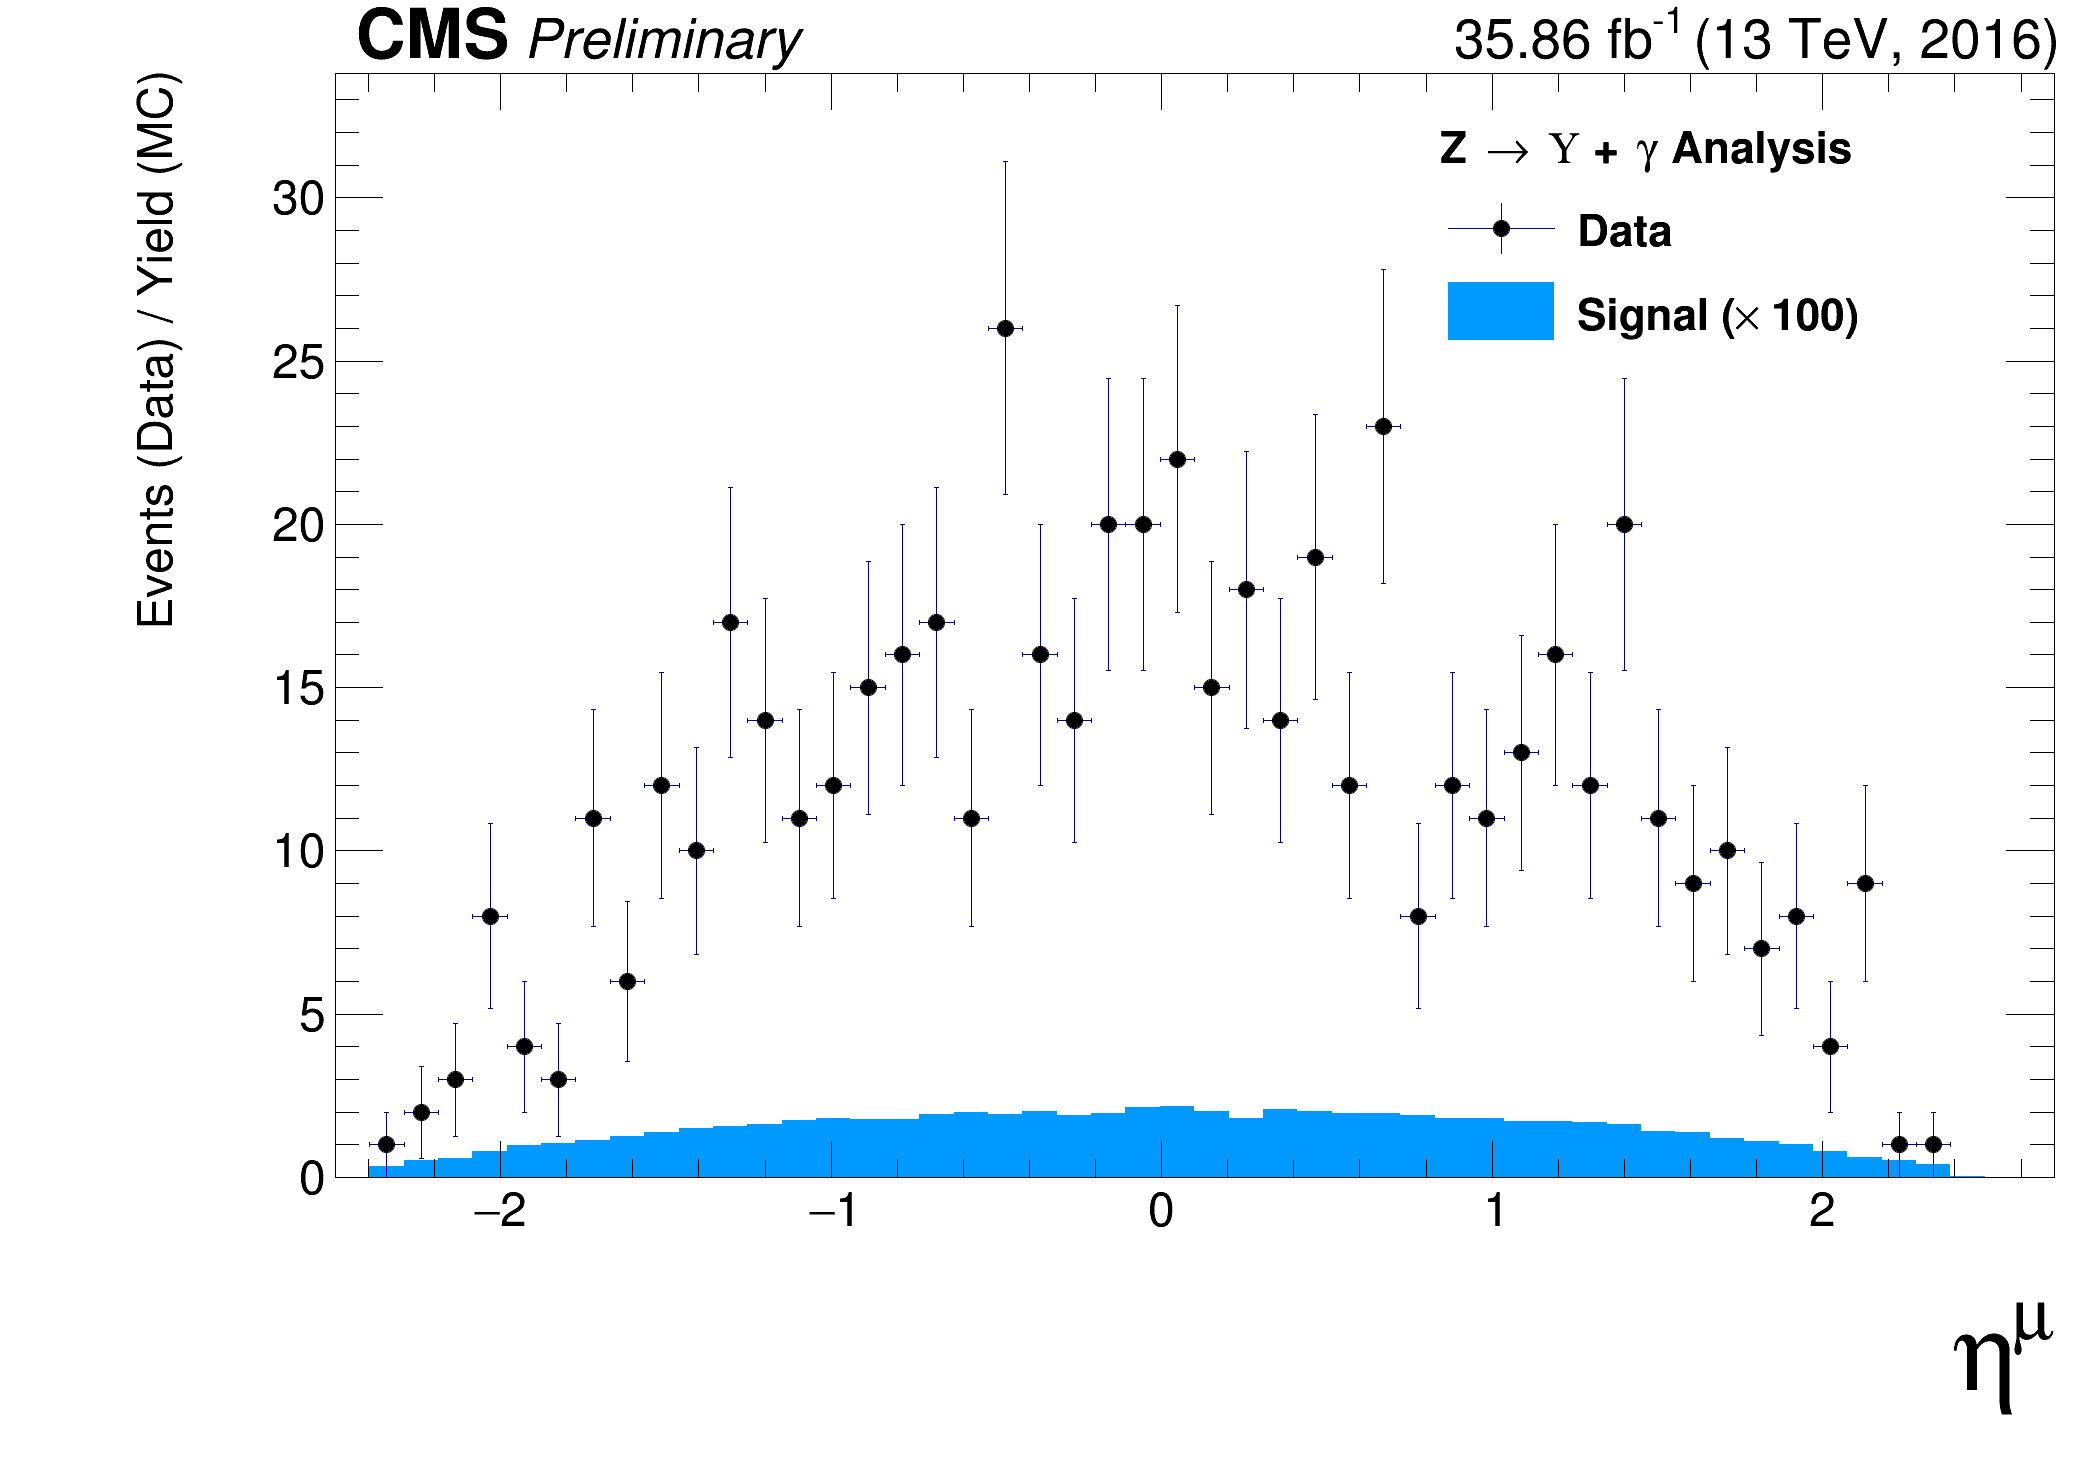
\includegraphics[width=0.45\textwidth]{figures_and_tables/outputPlots/ZtoUpsilon_Cat0_ZZZZZ/nEvts/data_x_mc/withKinCuts/h_withKin_LeadingMu_eta}
\end{center}\vspace*{-.5cm}
\caption{The $\eta$ muon distributions from data and signal events of Z decaying into $\Upsilon(1S,2S,3S)$ + $\gamma$ after Group I+II of selection cuts, where on left are presenting the trailing muons and on right are the leading muons. The plots are normalized to the number of events. Signal sample is scaled by a factor of $\times 100$). The black dots are data collect by CMS while the blue distribution is related only to the signal Monte-Carlo generated samples.}
\label{fig:etaMuons_ZtoUpsilon_Cat0_groupI_plus_II}
\end{figure}

%%%%%%%%% $\phi$ muon distributions for ZtoUpsilon_Cat0
\begin{figure}[!htbp]
\begin{center}
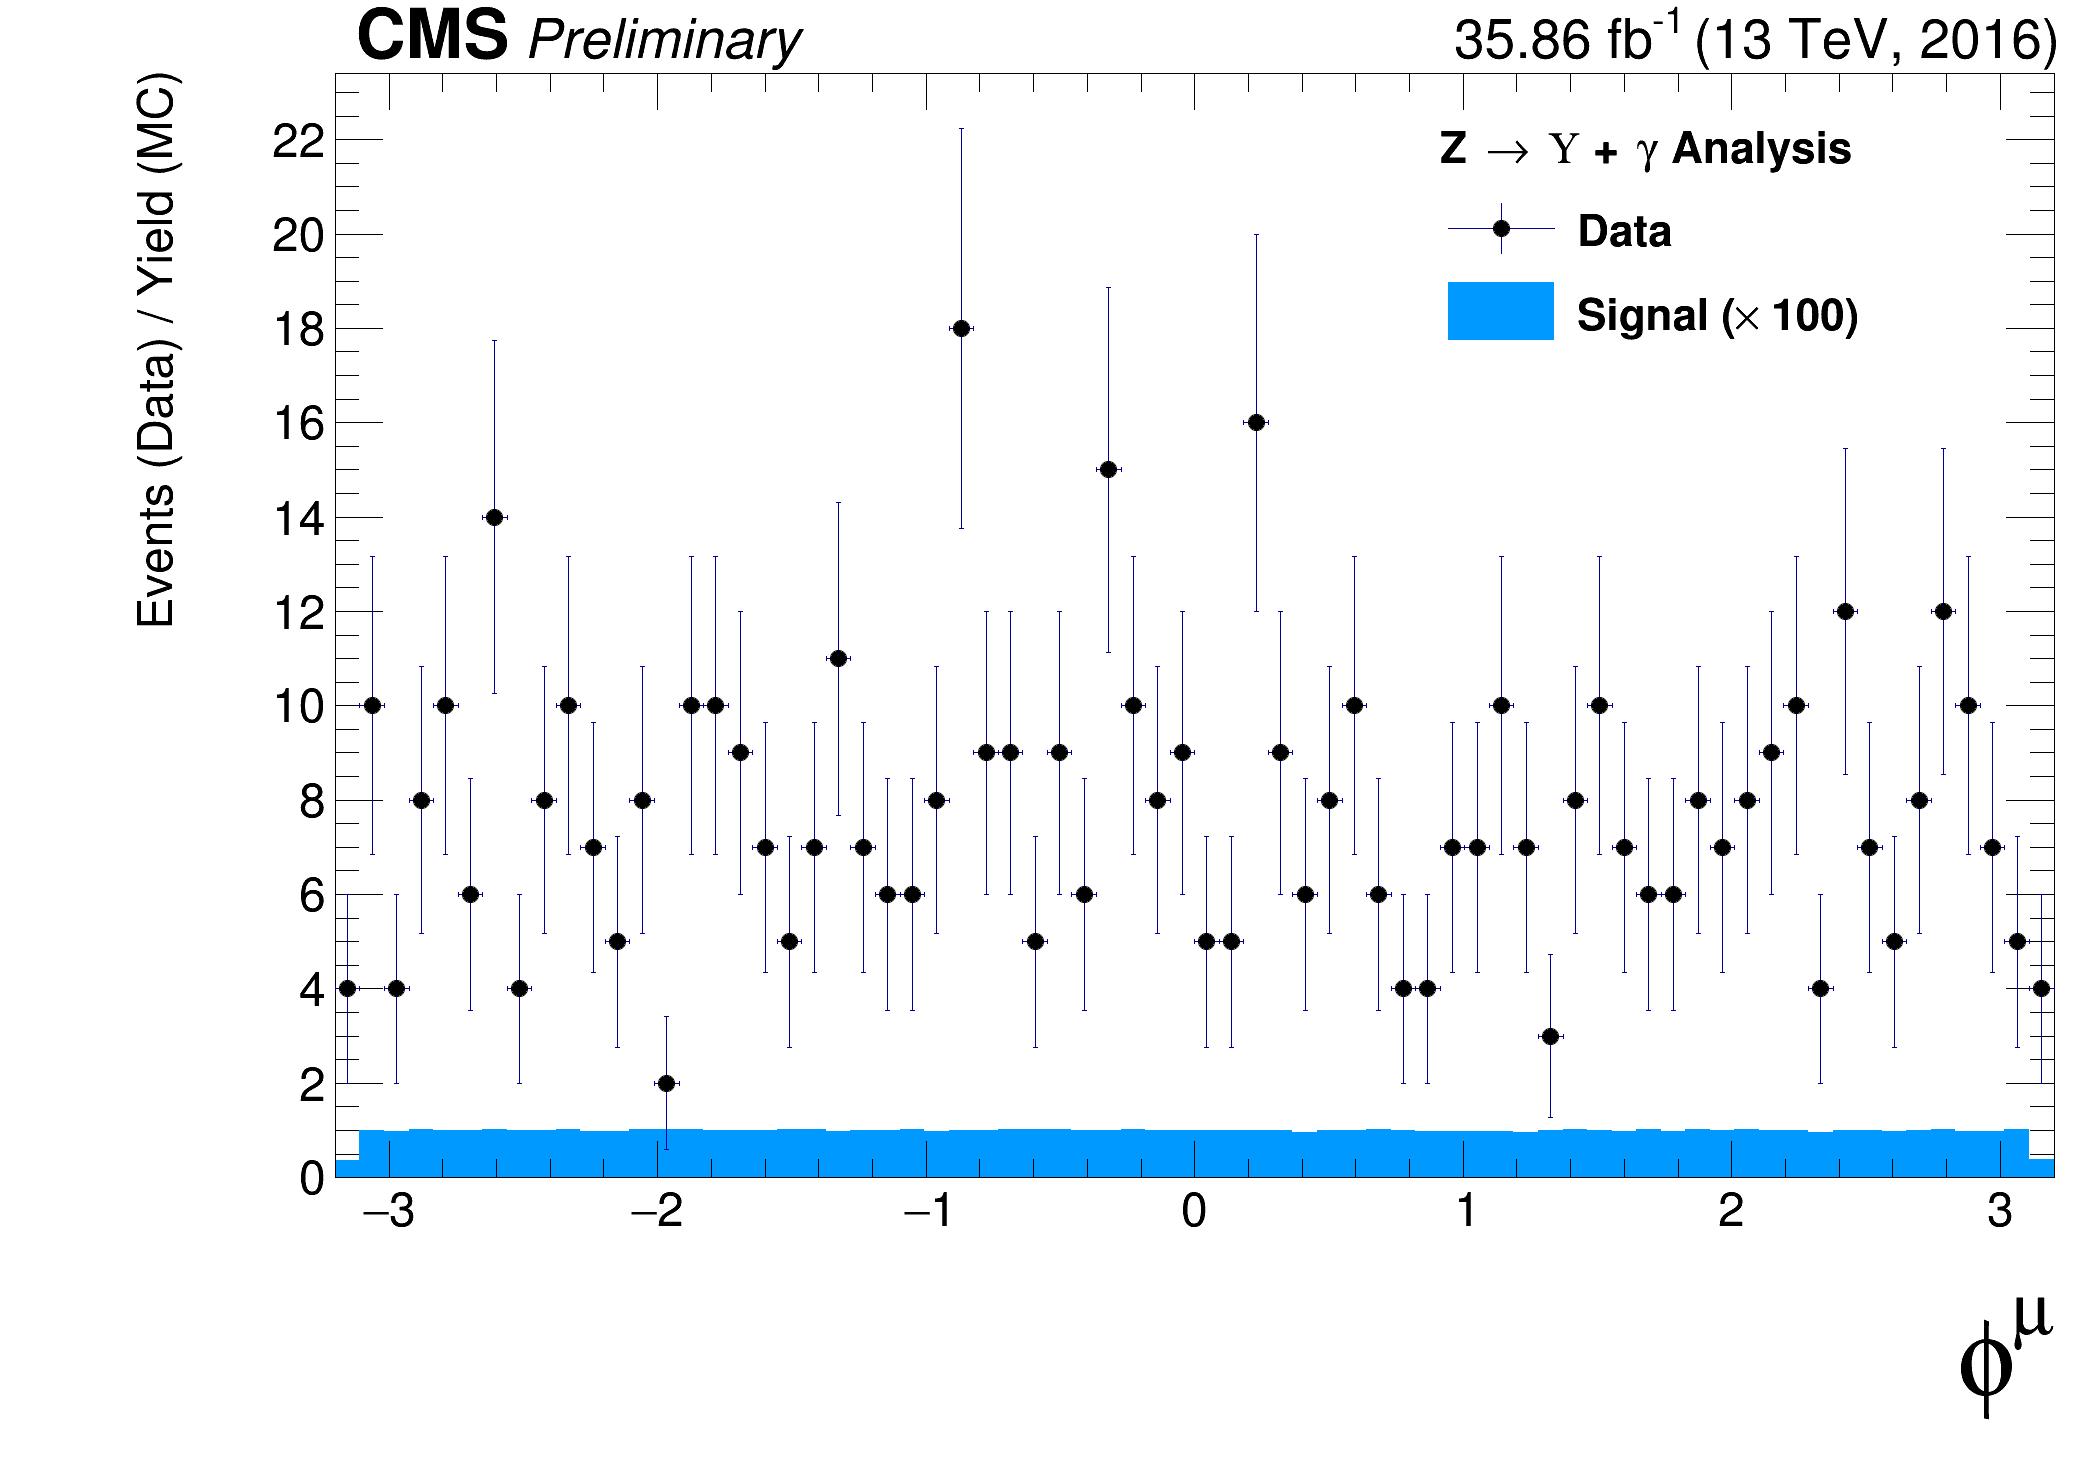
\includegraphics[width=0.45\textwidth]{figures_and_tables/outputPlots/ZtoUpsilon_Cat0_ZZZZZ/nEvts/data_x_mc/withKinCuts/h_withKin_TrailingMu_phi}\hspace*{1.cm}
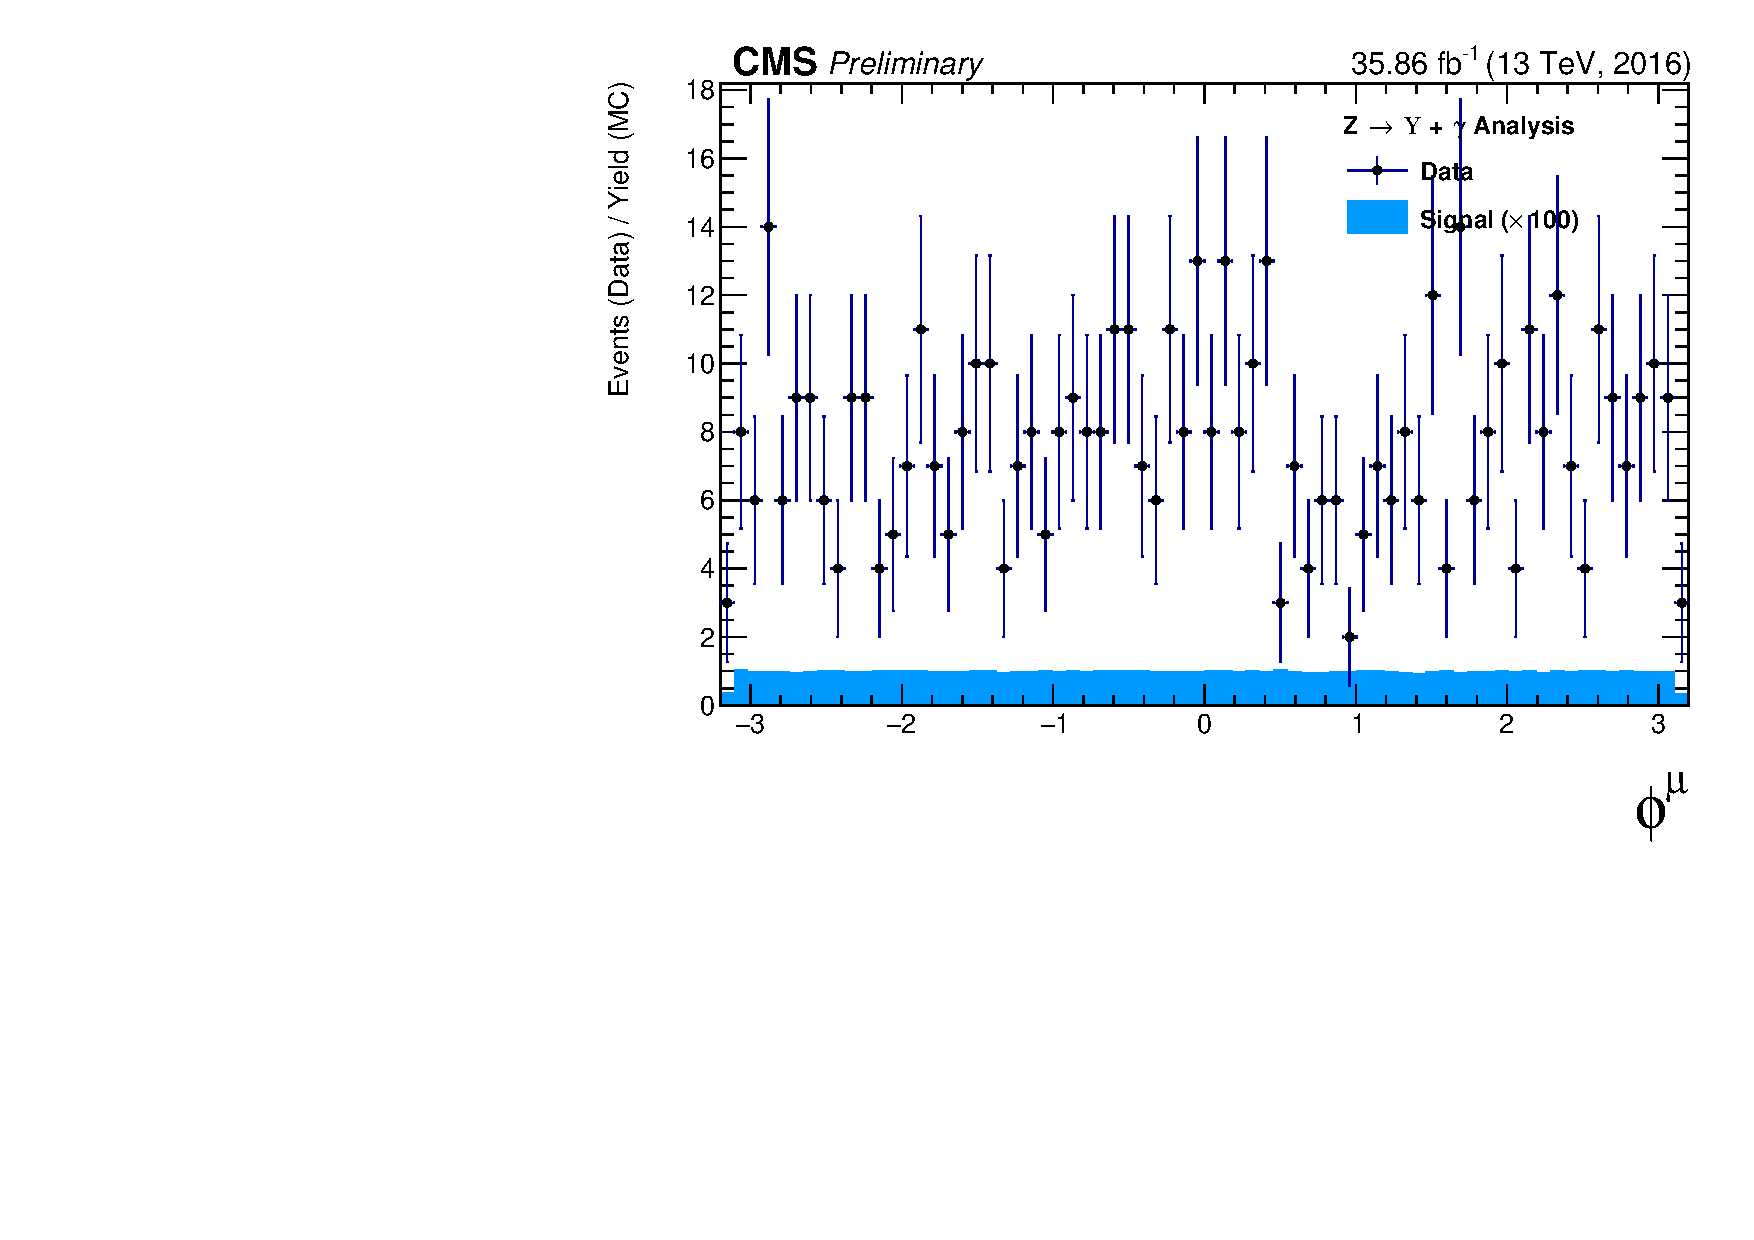
\includegraphics[width=0.45\textwidth]{figures_and_tables/outputPlots/ZtoUpsilon_Cat0_ZZZZZ/nEvts/data_x_mc/withKinCuts/h_withKin_LeadingMu_phi}
\end{center}\vspace*{-.5cm}
\caption{The $\phi$ muon distributions from data and signal events of Z decaying into $\Upsilon(1S,2S,3S)$ + $\gamma$ after Group I+II of selection cuts, where on left are presenting the trailing muons and on right are the leading muons. The plots are normalized to the number of events. Signal sample is scaled by a factor of $\times 100$). The black dots are data collect by CMS while the blue distribution is related only to the signal Monte-Carlo generated samples.}
\label{fig:phiMuons_ZtoUpsilon_Cat0_groupI_plus_II}
\end{figure}

%%%%%%%%%%%%%

%photon
%%$\pT$ Photon distributions for ZtoUpsilon_Cat0
\begin{figure}[!htbp]
\begin{center}
\includegraphics[width=0.45\textwidth]{figures_and_tables/outputPlots/ZtoUpsilon_Cat0_ZZZZZ/nEvts/data_x_mc/withKinCuts/h_withKin_Photon_pt}\hspace*{1.cm}
\end{center}\vspace*{-.5cm}
\caption{The \PT photon distributions from data and signal events for Z decaying into $\Upsilon(1S,2S,3S)$ + $\gamma$ all (Group I+II) selection cuts. The plot is normalized to the number of events. Signal sample is scaled by a factor of $\times 100$).}
\label{fig:pTPhoton_ZtoUpsilon_Cat0_groupI_plus_II}
\end{figure}


%%%%%%%$\eta$ Photon distributions for ZtoUpsilon_Cat0
\begin{figure}[!htbp]
\begin{center}
\includegraphics[width=0.45\textwidth]{figures_and_tables/outputPlots/ZtoUpsilon_Cat0_ZZZZZ/nEvts/data_x_mc/withKinCuts/h_withKin_Photon_eta}\hspace*{1.cm}
\end{center}\vspace*{-.5cm}
\caption{The $\eta$ photon distributions from data and signal events of Z decaying into $\Upsilon(1S,2S,3S)$ + $\gamma$ after all (Group I+II) selection cuts. The plot is normalized to the number of events. Signal sample is scaled by a factor of $\times 100$).}
\label{fig:etaPhoton_ZtoUpsilon_Cat0_groupI_plus_II}
\end{figure}

%%%%%%%%% $\phi$ Photon distributions for ZtoUpsilon_Cat0
\begin{figure}[!htbp]
\begin{center}
\includegraphics[width=0.45\textwidth]{figures_and_tables/outputPlots/ZtoUpsilon_Cat0_ZZZZZ/nEvts/data_x_mc/withKinCuts/h_withKin_Photon_phi}\hspace*{1.cm}
\end{center}\vspace*{-.5cm}
\caption{The $\phi$ photon distributions from data and signal events of Z decaying into $\Upsilon(1S,2S,3S)$ + $\gamma$ after all (Group I+II) selection cuts. The plot is normalized to the number of events. Signal sample is scaled by a factor of $\times 100$).}
\label{fig:phiPhoton_ZtoUpsilon_Cat0_groupI_plus_II}
\end{figure}

%%%%%%%%%%%%%
% Upsilon and Z boson
%%$\pT$ Upsilon_and_Higgs distributions for ZtoUpsilon_Cat0
\begin{figure}[!htbp]
\begin{center}
\includegraphics[width=0.45\textwidth]{figures_and_tables/outputPlots/ZtoUpsilon_Cat0_ZZZZZ/nEvts/data_x_mc/withKinCuts/h_withKin_Upsilon_Pt}\hspace*{1.cm}
\includegraphics[width=0.45\textwidth]{figures_and_tables/outputPlots/ZtoUpsilon_Cat0_ZZZZZ/nEvts/data_x_mc/withKinCuts/h_withKin_Z_Pt}
\end{center}\vspace*{-.5cm}
\caption{The \PT distributions for $\Upsilon(1S,2S,3S)$ in the left and for Z in the right from data and signal events for Z decaying into $\Upsilon(1S,2S,3S)$ + $\gamma$ after all (Group I+II) selection cuts. The plots are normalized to the number of events. Signal sample is scaled by a factor of $\times 100$). The black dots are data collect by CMS while the blue distribution is related only to the signal Monte-Carlo generated samples.}
\label{fig:pTUpsilon_and_Z_ZtoUpsilon_Cat0_groupI_plus_II}
\end{figure}


%%%%%%%$\eta$ Upsilon_and_Z distributions for ZtoUpsilon_Cat0
\begin{figure}[!htbp]
\begin{center}
\includegraphics[width=0.45\textwidth]{figures_and_tables/outputPlots/ZtoUpsilon_Cat0_ZZZZZ/nEvts/data_x_mc/withKinCuts/h_withKin_Upsilon_eta}\hspace*{1.cm}
\includegraphics[width=0.45\textwidth]{figures_and_tables/outputPlots/ZtoUpsilon_Cat0_ZZZZZ/nEvts/data_x_mc/withKinCuts/h_withKin_Z_eta}
\end{center}\vspace*{-.5cm}
\caption{The $\eta$ distributions for $\Upsilon(1S,2S,3S)$ in the left and for Z in the right from data and signal events for Z decaying into $\Upsilon(1S,2S,3S)$ + $\gamma$ after all (Group I+II) selection cuts. The plots are normalized to the number of events. Signal sample is scaled by a factor of $\times 100$). The black dots are data collect by CMS while the blue distribution is related only to the signal Monte-Carlo generated samples.}
\label{fig:etaUpsilon_and_Z_ZtoUpsilon_Cat0_groupI_plus_II}
\end{figure}

%%%%%%%%% $\phi$ Upsilon_and_Zdistributions for ZtoUpsilon_Cat0
\begin{figure}[!htbp]
\begin{center}
\includegraphics[width=0.45\textwidth]{figures_and_tables/outputPlots/ZtoUpsilon_Cat0_ZZZZZ/nEvts/data_x_mc/withKinCuts/h_withKin_Upsilon_phi}\hspace*{1.cm}
\includegraphics[width=0.45\textwidth]{figures_and_tables/outputPlots/ZtoUpsilon_Cat0_ZZZZZ/nEvts/data_x_mc/withKinCuts/h_withKin_Z_phi}
\end{center}\vspace*{-.5cm}
\caption{The $\phi$ distributions for $\Upsilon(1S,2S,3S)$ in the left and for Z in the right from data and signal events for Z decaying into $\Upsilon(1S,2S,3S)$ + $\gamma$ after all (Group I+II) selection cuts. The plots are normalized to the number of events. Signal sample is scaled by a factor of $\times 100$). The black dots are data collect by CMS while the blue distribution is related only to the signal Monte-Carlo generated samples.}
\label{fig:phiUpsilon_and_Z_ZtoUpsilon_Cat0_groupI_plus_II}
\end{figure}

%%%%%%%%%%%%

%%%%%%%%%%%%%
% kin cuts
%% delta R -  mu x photon distributions for ZtoUpsilon_Cat0
\begin{figure}[!htbp]
\begin{center}
\includegraphics[width=0.45\textwidth]{figures_and_tables/outputPlots/ZtoUpsilon_Cat0_ZZZZZ/nEvts/data_x_mc/withKinCuts/h_withKin_deltaR_Leading_Photon}\hspace*{1.cm}
\includegraphics[width=0.45\textwidth]{figures_and_tables/outputPlots/ZtoUpsilon_Cat0_ZZZZZ/nEvts/data_x_mc/withKinCuts/h_withKin_deltaR_Trailing_Photon}\end{center}\vspace*{-.5cm}
\caption{The $\Delta R$ distributions between the photon and the leading muon (left) and the trailing muon (right) for $\Upsilon(1S,2S,3S)$ from data and signal events for Z decaying after all (Group I+II) selection cuts. The plots are normalized to the number of events. Signal sample is scaled by a factor of $\times 100$). The black dots are data collect by CMS while the blue distribution is related only to the signal Monte-Carlo generated samples.}
\label{fig:deltaR_ZtoUpsilon_Cat0_groupI_plus_II}
\end{figure}


%%%%%%% energy/mass ratio distributions for ZtoUpsilon_Cat0
\begin{figure}[!htbp]
\begin{center}
\includegraphics[width=0.45\textwidth]{figures_and_tables/outputPlots/ZtoUpsilon_Cat0_ZZZZZ/nEvts/data_x_mc/withKinCuts/h_withKin_upsilonPt_over_zMass}\hspace*{1.cm}
\includegraphics[width=0.45\textwidth]{figures_and_tables/outputPlots/ZtoUpsilon_Cat0_ZZZZZ/nEvts/data_x_mc/withKinCuts/h_withKin_photonPt_over_zMass}
\end{center}\vspace*{-.5cm}
\caption{The ratio for the transverse momentum of the reconstructed Upsilon and the reconstructed Z mass ($p_{T}^{\mu\mu}/M_{\mu\mu\gamma}$ - left) and the ratio for the transverse energy of the reconstructed Photon and the reconstructed Z mass ($E_{T}^{\gamma}/M_{\mu\mu\gamma}$ - right) distribution for $\Upsilon(1S,2S,3S)$ from data and signal events for Z decaying after all (Group I+II) selection cuts. The plots are normalized to the number of events. Signal sample is scaled by a factor of $\times 100$). The black dots are data collect by CMS while the blue distribution is related only to the signal Monte-Carlo generated samples.}
\label{fig:energy_ration_ZtoUpsilon_Cat0_groupI_plus_II}
\end{figure}

%%%%%%%%%% dimuon mass distributions for ZtoUpsilon_Cat0
%\begin{figure}[!htbp]
%\begin{center}
%\includegraphics[width=0.45\textwidth]{figures_and_tables/outputPlots/ZtoUpsilon_Cat0_ZZZZZ/nEvts/data_x_mc/withKinCuts/h_withKin_Upsilon_Mass_Signal_and_Background_LargeRange}\hspace*{1.cm}
%\end{center}\vspace*{-.5cm}
%\caption{The dimuon mass distribution of the reconstructed $\Upsilon (1S,2S,3S)$ from data and signal events for Z decaying after all (Group I+II) selection cuts. The plot is normalized to the number of events. Signal sample is scaled by a factor of $\times 100$).}
%\label{fig:dimuon_mass_ZtoUpsilon_Cat0_groupI_plus_II}
%\end{figure}

%%%%%%%%%%%%



%CONTROL PLOTS
%%$\pT$ muon distributions for HtoUpsilon_Cat0
\begin{figure}[!htbp]
\begin{center}
\includegraphics[width=0.45\textwidth]{figures_and_tables/outputPlots/HtoUpsilon_Cat0_ZZZZZ/nEvts/data_x_mc/withKinCuts/h_withKin_TrailingMu_pt}\hspace*{1.cm}
\includegraphics[width=0.45\textwidth]{figures_and_tables/outputPlots/HtoUpsilon_Cat0_ZZZZZ/nEvts/data_x_mc/withKinCuts/h_withKin_LeadingMu_pt}
\end{center}\vspace*{-.5cm}
\caption{The \PT muon distributions from data and signal events for Higgs decaying into $\Upsilon(1S,2S,3S)$ + $\gamma$ after Group I of selection cuts, where on left are presenting the trailing muons and on right are the leading muons. The plots are normalized to the number of events. Signal sample is scaled by a factor of $\times 600000$). The black dots are data collect by CMS while the blue distribution is related only to the signal Monte-Carlo generated samples.}
\label{fig:pTMuons_HtoUpsilon_Cat0_groupI_plus_II}
\end{figure}


%%%%%%%$\eta$ muon distributions for HtoUpsilon_Cat0
\begin{figure}[!htbp]
\begin{center}
\includegraphics[width=0.45\textwidth]{figures_and_tables/outputPlots/HtoUpsilon_Cat0_ZZZZZ/nEvts/data_x_mc/withKinCuts/h_withKin_TrailingMu_eta}\hspace*{1.cm}
\includegraphics[width=0.45\textwidth]{figures_and_tables/outputPlots/HtoUpsilon_Cat0_ZZZZZ/nEvts/data_x_mc/withKinCuts/h_withKin_LeadingMu_eta}
\end{center}\vspace*{-.5cm}
\caption{The $\eta$ muon distributions from data and signal events of Higgs decaying into $\Upsilon(1S,2S,3S)$ + $\gamma$ after Group I of selection cuts, where on left are presenting the trailing muons and on right are the leading muons. The plots are normalized to the number of events. Signal sample is scaled by a factor of $\times 600000$). The black dots are data collect by CMS while the blue distribution is related only to the signal Monte-Carlo generated samples.}
\label{fig:etaMuons_HtoUpsilon_Cat0_groupI_plus_II}
\end{figure}

%%%%%%%%% $\phi$ muon distributions for HtoUpsilon_Cat0
\begin{figure}[!htbp]
\begin{center}
\includegraphics[width=0.45\textwidth]{figures_and_tables/outputPlots/HtoUpsilon_Cat0_ZZZZZ/nEvts/data_x_mc/withKinCuts/h_withKin_TrailingMu_phi}\hspace*{1.cm}
\includegraphics[width=0.45\textwidth]{figures_and_tables/outputPlots/HtoUpsilon_Cat0_ZZZZZ/nEvts/data_x_mc/withKinCuts/h_withKin_LeadingMu_phi}
\end{center}\vspace*{-.5cm}
\caption{The $\phi$ muon distributions from data and signal events of Higgs decaying into $\Upsilon(1S,2S,3S)$ + $\gamma$ after Group I of selection cuts, where on left are presenting the trailing muons and on right are the leading muons. The plots are normalized to the number of events. Signal sample is scaled by a factor of $\times 600000$). The black dots are data collect by CMS while the blue distribution is related only to the signal Monte-Carlo generated samples.}
\label{fig:phiMuons_HtoUpsilon_Cat0_groupI_plus_II}
\end{figure}

%%%%%%%%%%%%%

%photon
%%$\pT$ Photon distributions for HtoUpsilon_Cat0
\begin{figure}[!htbp]
\begin{center}
\includegraphics[width=0.45\textwidth]{figures_and_tables/outputPlots/HtoUpsilon_Cat0_ZZZZZ/nEvts/data_x_mc/withKinCuts/h_withKin_Photon_pt}\hspace*{1.cm}
\end{center}\vspace*{-.5cm}
\caption{The \PT photon distributions from data and signal events for Higgs decaying into $\Upsilon(1S,2S,3S)$ + $\gamma$ all (Group I+II) selection cuts. The plot is normalized to the number of events. Signal sample is scaled by a factor of $\times 600000$).}
\label{fig:pTPhoton_HtoUpsilon_Cat0_groupI_plus_II}
\end{figure}


%%%%%%%$\eta$ Photon distributions for HtoUpsilon_Cat0
\begin{figure}[!htbp]
\begin{center}
\includegraphics[width=0.45\textwidth]{figures_and_tables/outputPlots/HtoUpsilon_Cat0_ZZZZZ/nEvts/data_x_mc/withKinCuts/h_withKin_Photon_eta}\hspace*{1.cm}
\end{center}\vspace*{-.5cm}
\caption{The $\eta$ photon distributions from data and signal events of Higgs decaying into $\Upsilon(1S,2S,3S)$ + $\gamma$ after all (Group I+II) selection cuts. The plot is normalized to the number of events. Signal sample is scaled by a factor of $\times 600000$).}
\label{fig:etaPhoton_HtoUpsilon_Cat0_groupI_plus_II}
\end{figure}

%%%%%%%%% $\phi$ Photon distributions for HtoUpsilon_Cat0
\begin{figure}[!htbp]
\begin{center}
\includegraphics[width=0.45\textwidth]{figures_and_tables/outputPlots/HtoUpsilon_Cat0_ZZZZZ/nEvts/data_x_mc/withKinCuts/h_withKin_Photon_phi}\hspace*{1.cm}
\end{center}\vspace*{-.5cm}
\caption{The $\phi$ photon distributions from data and signal events of Higgs decaying into $\Upsilon(1S,2S,3S)$ + $\gamma$ after all (Group I+II) selection cuts. The plot is normalized to the number of events. Signal sample is scaled by a factor of c).}
\label{fig:phiPhoton_HtoUpsilon_Cat0_groupI_plus_II}
\end{figure}

%%%%%%%%%%%%%
% Upsilon and Higgs boson
%%$\pT$ Upsilon_and_Higgs distributions for HtoUpsilon_Cat0
\begin{figure}[!htbp]
\begin{center}
\includegraphics[width=0.45\textwidth]{figures_and_tables/outputPlots/HtoUpsilon_Cat0_ZZZZZ/nEvts/data_x_mc/withKinCuts/h_withKin_Upsilon_Pt}\hspace*{1.cm}
\includegraphics[width=0.45\textwidth]{figures_and_tables/outputPlots/HtoUpsilon_Cat0_ZZZZZ/nEvts/data_x_mc/withKinCuts/h_withKin_Z_Pt}
\end{center}\vspace*{-.5cm}
\caption{The \PT distributions for $\Upsilon(1S,2S,3S)$ in the left and for Higgs in the right from data and signal events for Higgs decaying into $\Upsilon(1S,2S,3S)$ + $\gamma$ after all (Group I+II) selection cuts. The plots are normalized to the number of events. Signal sample is scaled by a factor of $\times 600000$). The black dots are data collect by CMS while the blue distribution is related only to the signal Monte-Carlo generated samples.}
\label{fig:pTUpsilon_and_Higgs_HtoUpsilon_Cat0_groupI_plus_II}
\end{figure}


%%%%%%%$\eta$ Upsilon_and_Higgs distributions for HtoUpsilon_Cat0
\begin{figure}[!htbp]
\begin{center}
\includegraphics[width=0.45\textwidth]{figures_and_tables/outputPlots/HtoUpsilon_Cat0_ZZZZZ/nEvts/data_x_mc/withKinCuts/h_withKin_Upsilon_eta}\hspace*{1.cm}
\includegraphics[width=0.45\textwidth]{figures_and_tables/outputPlots/HtoUpsilon_Cat0_ZZZZZ/nEvts/data_x_mc/withKinCuts/h_withKin_Z_eta}
\end{center}\vspace*{-.5cm}
\caption{The $\eta$ distributions for $\Upsilon(1S,2S,3S)$ in the left and for Higgs in the right from data and signal events for Higgs decaying into $\Upsilon(1S,2S,3S)$ + $\gamma$ after all (Group I+II) selection cuts. The plots are normalized to the number of events. Signal sample is scaled by a factor of $\times 600000$). The black dots are data collect by CMS while the blue distribution is related only to the signal Monte-Carlo generated samples.}
\label{fig:etaUpsilon_and_Higgs_HtoUpsilon_Cat0_groupI_plus_II}
\end{figure}

%%%%%%%%% $\phi$ Upsilon_and_Higgsdistributions for HtoUpsilon_Cat0
\begin{figure}[!htbp]
\begin{center}
\includegraphics[width=0.45\textwidth]{figures_and_tables/outputPlots/HtoUpsilon_Cat0_ZZZZZ/nEvts/data_x_mc/withKinCuts/h_withKin_Upsilon_phi}\hspace*{1.cm}
\includegraphics[width=0.45\textwidth]{figures_and_tables/outputPlots/HtoUpsilon_Cat0_ZZZZZ/nEvts/data_x_mc/withKinCuts/h_withKin_Z_phi}
\end{center}\vspace*{-.5cm}
\caption{The $\phi$ distributions for $\Upsilon(1S,2S,3S)$ in the left and for Higgs in the right from data and signal events for Higgs decaying into $\Upsilon(1S,2S,3S)$ + $\gamma$ after all (Group I+II) selection cuts. The plots are normalized to the number of events. Signal sample is scaled by a factor of $\times 600000$). The black dots are data collect by CMS while the blue distribution is related only to the signal Monte-Carlo generated samples.}
\label{fig:phiUpsilon_and_Higgs_HtoUpsilon_Cat0_groupI_plus_II}
\end{figure}

%%%%%%%%%%%%

%%%%%%%%%%%%%
% kin cuts
%% delta R -  mu x photon distributions for HtoUpsilon_Cat0
\begin{figure}[!htbp]
\begin{center}
\includegraphics[width=0.45\textwidth]{figures_and_tables/outputPlots/HtoUpsilon_Cat0_ZZZZZ/nEvts/data_x_mc/withKinCuts/h_withKin_deltaR_Leading_Photon}\hspace*{1.cm}
\includegraphics[width=0.45\textwidth]{figures_and_tables/outputPlots/HtoUpsilon_Cat0_ZZZZZ/nEvts/data_x_mc/withKinCuts/h_withKin_deltaR_Trailing_Photon}\end{center}\vspace*{-.5cm}
\caption{The $\Delta R$ distributions between the photon and the leading muon (left) and the trailing muon (right) for $\Upsilon(1S,2S,3S)$ from data and signal events for Higgs decaying after all (Group I+II) selection cuts. The plots are normalized to the number of events. Signal sample is scaled by a factor of $\times 600000$). The black dots are data collect by CMS while the blue distribution is related only to the signal Monte-Carlo generated samples.}
\label{fig:deltaR_HtoUpsilon_Cat0_groupI_plus_II}
\end{figure}


%%%%%%% energy/mass ratio distributions for HtoUpsilon_Cat0
\begin{figure}[!htbp]
\begin{center}
\includegraphics[width=0.45\textwidth]{figures_and_tables/outputPlots/HtoUpsilon_Cat0_ZZZZZ/nEvts/data_x_mc/withKinCuts/h_withKin_upsilonPt_over_zMass}\hspace*{1.cm}
\includegraphics[width=0.45\textwidth]{figures_and_tables/outputPlots/HtoUpsilon_Cat0_ZZZZZ/nEvts/data_x_mc/withKinCuts/h_withKin_photonPt_over_zMass}
\end{center}\vspace*{-.5cm}
\caption{The ratio for the transverse momentum of the reconstructed Upsilon and the reconstructed Higgs mass ($p_{T}^{\mu\mu}/M_{\mu\mu\gamma}$ - left) and the ratio for the transverse energy of the reconstructed Photon and the reconstructed Higgs mass ($E_{T}^{\gamma}/M_{\mu\mu\gamma}$ - right) distribution for $\Upsilon(1S,2S,3S)$ from data and signal events for Higgs decaying after all (Group I+II) selection cuts. The plots are normalized to the number of events. Signal sample is scaled by a factor of $\times 600000$). The black dots are data collect by CMS while the blue distribution is related only to the signal Monte-Carlo generated samples.}
\label{fig:energy_ration_HtoUpsilon_Cat0_groupI_plus_II}
\end{figure}

%%%%%%%%%% dimuon mass distributions for HtoUpsilon_Cat0
%\begin{figure}[!htbp]
%\begin{center}
%\includegraphics[width=0.45\textwidth]{figures_and_tables/outputPlots/HtoUpsilon_Cat0_ZZZZZ/nEvts/data_x_mc/withKinCuts/h_withKin_Upsilon_Mass_Signal_and_Background_LargeRange}\hspace*{1.cm}
%\end{center}\vspace*{-.5cm}
%\caption{The dimuon mass distribution of the reconstructed $\Upsilon (1S,2S,3S)$ from data and signal events for Higgs decaying after all (Group I+II) selection cuts.}
%\label{fig:dimuon_mass_HtoUpsilon_Cat0_groupI_plus_II}
%\end{figure}

%%%%%%%%%%%%%%%%%%%%%%%%%%%%%%%%%%%%%%%%%%%%%%%%%%%%%%%%%%%%%%%%%%%%%%%%%%%%%%%%%%%%%%%%%%%%%%%%%%%%%%%%%
%%%%%%%%%%%%%%%%%%%%%%%%%%%%%%%%%%%%%%%%%%%%%%%%%%%%%%%%%%%%%%%%%%%%%%%%%%%%%%%%%%%%%%%%%%%%%%%%%%%%%%%%%
%%%%%%%%%%%%%%%%%%%%%%%%%%%%%%%%%%%%%%%%%%%%%%%%%%%%%%%%%%%%%%%%%%%%%%%%%%%%%%%%%%%%%%%%%%%%%%%%%%%%%%%%%
%%%%%%%%%%%%%%%%%%%%%%%%%%%%%%%%%%%%%%%%%%%%%%%%%%%%%%%%%%%%%%%%%%%%%%%%%%%%%%%%%%%%%%%%%%%%%%%%%%%%%%%%%
%%%%%%%%%%%%%%%%%%%%%%%%%%%%%%%%%%%%%%%%%%%%%%%%%%%%%%%%%%%%%%%%%%%%%%%%%%%%%%%%%%%%%%%%%%%%%%%%%%%%%%%%%
%%%%%%%%%%%%%%%%%%%%%%%%%%%%%%%%%%%%%%%%%%%%%%%%%%%%%%%%%%%%%%%%%%%%%%%%%%%%%%%%%%%%%%%%%%%%%%%%%%%%%%%%%
%%%%%%%%%%%%%%%%%%%%%%%%%%%%%%%%%%%%%%%%%%%%%%%%%%%%%%%%%%%%%%%%%%%%%%%%%%%%%%%%%%%%%%%%%%%%%%%%%%%%%%%%%
%%%%%%%%%%%%%%%%%%%%%%%%%%%%%%%%%%%%%%%%%%%%%%%%%%%%%%%%%%%%%%%%%%%%%%%%%%%%%%%%%%%%%%%%%%%%%%%%%%%%%%%%%
%%%%%%%%%%%%%%%%%%%%%%%%%%%%%%%%%%%%%%%%%%%%%%%%%%%%%%%%%%%%%%%%%%%%%%%%%%%%%%%%%%%%%%%%%%%%%%%%%%%%%%%%%
%%%%%%%%%%%%%%%%%%%%%%%%%%%%%%%%%%%%%%%%%%%%%%%%%%%%%%%%%%%%%%%%%%%%%%%%%%%%%%%%%%%%%%%%%%%%%%%%%%%%%%%%%
%%%%%%%%%%%%%%%%%%%%%%%%%%%%%%%%%%%%%%%%%%%%%%%%%%%%%%%%%%%%%%%%%%%%%%%%%%%%%%%%%%%%%%%%%%%%%%%%%%%%%%%%%
%             _ _     _     
%            (_) |   | |    
%  _   _  ___ _| | __| |___ 
% | | | |/ _ \ | |/ _` / __|
% | |_| |  __/ | | (_| \__ \
%  \__, |\___|_|_|\__,_|___/
%   __/ |                   
%  |___/                    
%%%%%%%%%%%%%%%%%%%%%%%%%%%%%%%%%%%%%%%%%%%%%%%%%%%%%%%%%%%%%%%%%%%%%%%%%%%%%%%%%%%%%%%%%%%%%%%%%%%%%%%%%
%%%%%%%%%%%%%%%%%%%%%%%%%%%%%%%%%%%%%%%%%%%%%%%%%%%%%%%%%%%%%%%%%%%%%%%%%%%%%%%%%%%%%%%%%%%%%%%%%%%%%%%%%
%%%%%%%%%%%%%%%%%%%%%%%%%%%%%%%%%%%%%%%%%%%%%%%%%%%%%%%%%%%%%%%%%%%%%%%%%%%%%%%%%%%%%%%%%%%%%%%%%%%%%%%%%
%%%%%%%%%%%%%%%%%%%%%%%%%%%%%%%%%%%%%%%%%%%%%%%%%%%%%%%%%%%%%%%%%%%%%%%%%%%%%%%%%%%%%%%%%%%%%%%%%%%%%%%%%
%%%%%%%%%%%%%%%%%%%%%%%%%%%%%%%%%%%%%%%%%%%%%%%%%%%%%%%%%%%%%%%%%%%%%%%%%%%%%%%%%%%%%%%%%%%%%%%%%%%%%%%%%
%%%%%%%%%%%%%%%%%%%%%%%%%%%%%%%%%%%%%%%%%%%%%%%%%%%%%%%%%%%%%%%%%%%%%%%%%%%%%%%%%%%%%%%%%%%%%%%%%%%%%%%%%
%%%%%%%%%%%%%%%%%%%%%%%%%%%%%%%%%%%%%%%%%%%%%%%%%%%%%%%%%%%%%%%%%%%%%%%%%%%%%%%%%%%%%%%%%%%%%%%%%%%%%%%%%
%%%%%%%%%%%%%%%%%%%%%%%%%%%%%%%%%%%%%%%%%%%%%%%%%%%%%%%%%%%%%%%%%%%%%%%%%%%%%%%%%%%%%%%%%%%%%%%%%%%%%%%%%
%%%%%%%%%%%%%%%%%%%%%%%%%%%%%%%%%%%%%%%%%%%%%%%%%%%%%%%%%%%%%%%%%%%%%%%%%%%%%%%%%%%%%%%%%%%%%%%%%%%%%%%%%
%%%%%%%%%%%%%%%%%%%%%%%%%%%%%%%%%%%%%%%%%%%%%%%%%%%%%%%%%%%%%%%%%%%%%%%%%%%%%%%%%%%%%%%%%%%%%%%%%%%%%%%%%



\clearpage
\section{Event categorization and yields}
\label{sec:categorization}

In order to increase the sensibility of the analysis, a categorization procedure was applied.
 % Table \ref{tab:categorization} present the 3 exclusive categories proposed. 
 They are based on the $\eta$ and R9 distribution of the reconstructed photon.

The photon R9 is a shower shape variable defined as the fraction of energy deposited in the 5x5 square surrounding the Super Cluster seed of the reconstructed photon. A photon that convert before reaching the ECAL tend to have lower values of R9, in comparison with unconverted photons. Converted photons have wider energy resolution and are more likely to be misidentified.

% \begin{table}[ht]
% \begin{center}

% \begin{tabular}{l|l}

% \textbf{Name} & \textbf{Definition} \\ \hline
% Cat0 & No categorization.                     \\ \hline
% EB High R9 & $|\eta_{SC}| < 1.444$ (Barrel)         \\
%      & $R9 >$ 0.94 (High R9)                           \\ \hline
% EB Low R9 & $|\eta_{SC}| < 1.444$ (Barrel)         \\
%      & $R9 <$ 0.94 (Low R9)                            \\ \hline
% EE & $1.566 < |\eta_{SC}| < 2.5$ (Endcap)   \\
%      & No R9 categorization.                  \\ 
% \end{tabular}


% \caption{Exclusive categories implemented based on the reconstructed photon. The uncategorized selection (Cat0) is the sum of the three categories and, for the \Z decay, it is kept only for reference. For the Higgs decay, it is actually used for the limits extraction.}
% \label{tab:categorization}
% \end{center}
% \end{table}

Selected events with the photon reconstructed inside the barrel and with $R9 > 0.94$ are categorized as "EB High R9"~\footnote{EB stands for Electromagnetic Barrel}, selected events with the photon reconstructed inside the barrel and with $R9 < 0.94$ are categorized as "EB Low R9" and selected events with the photon reconstructed inside the endcap, regardless of its R9 value, categorized as "EE". This categorization is done in view of increase the analysis sensitivity. 

This categorization is implemented only for the \Z decay. The Higgs does not present enough statistics to make it profitable, so only the inclusive one is used. 

\subsection{R9 reweighting}

As spotted by the $H \rightarrow \gamma\gamma$ analysis, during Run1~\cite{higgs_gammagamma_PAPPER}, there is a disagreement in the R9 distribution of photons in Data and MC. In order to mitigate this difference, a transformation factor is extracted and applied to the reconstructed photons before the categorization.

The same approach of the $H \rightarrow \gamma\gamma$ analysis is applied, in which the nominal photon selection of this analysis (see section \ref{sec:photon_id}) is used to select photons on Data and MC. Then the two distributions are remapped and the transformation factors are extracted. 

Figure \ref{fig:r9_reweighting} show the R9 distribution before and after the reweighting, for the Barrel and the Endcap.

%%%%%%%%% R9
% more info: https://eliza.web.cern.ch/eliza/public/ZGTo2MuG_MMuMu_EraDcutsR9/

\begin{figure}[!htbp]
\begin{center}
\includegraphics[width=0.45\textwidth]{figures_and_tables/R9/R9EB.png}\hspace*{1.cm}
\includegraphics[width=0.45\textwidth]{figures_and_tables/R9/R9EE.png}
\end{center}\vspace*{-.5cm}
\caption{Data and MC of the R9 variable, before and after the reweighting. Barrel (left) and Endcap (right).}
\label{fig:r9_reweighting}
\end{figure}

\subsection{Event counting and yields}
\label{sec:yields}

Tables \ref{tab:Z_yields} and \ref{tab:HIGGS_yields} show the total number of events before and after the full selection. Two things are important to notice.

\begin{table}[ht]
\begin{center}
  \caption{Number of events for the Z decay, before and after the full selection, per categorization scenarios.}



\begin{tabular}{c|c|c|c|c|c}
%& \multicolumn{5}{c}{$Z \rightarrow \Upsilon(1S, 2S, 3S)+\gamma$}       \\
\hline
\hline

&  &  \multicolumn{3}{c|}{Signal $Z \rightarrow \Upsilon(nS)+\gamma$} &    \\
\cline{3-5}
& Data & $n=1$ & $n=2$ & $n=3$ &  $Z \rightarrow \mu\mu\gamma_{FSR}$  \\
\hline
Total & 169.84 M &  3.54 & 1.4 & 1.22 & $3.33 \times 10^{3}$  \\
\hline\hline
Inclusive & 447  &  0.393 &  0.157 &  0.136 &  176  \\
EB High R9 & 197  &  0.172 &  0.0682 &  0.0597 &  78  \\
EB Low R9 & 146  &  0.129 &  0.0519 &  0.0448 &  58.5  \\
EE & 104  &  0.0916 &  0.0365 &  0.032 &  39.8 \\

\end{tabular}


\label{tab:Z_yields}
\end{center}
\end{table}


\begin{table}[ht]
\caption{Number of events for the H decay, before and after the full selection.}
\begin{center}


\begin{tabular}{c|c|c|c|c|c}
%& \multicolumn{5}{c}{$H \rightarrow \Upsilon(1S, 2S, 3S)+\gamma$}       \\
\hline
\hline

&  &  \multicolumn{3}{c|}{Signal $H \rightarrow \Upsilon(nS)+\gamma$} &    \\
\cline{3-5}
& Data & $n=1$ & $n=2$ & $n=3$ &  $H \rightarrow \gamma\gamma^{*}$  \\
\hline
Total & 169.84 M &  0.000257 & $5.43 \times 10^{-5}$ & $3.93 \times 10^{-5}$ & 136  \\
\hline\hline
Inclusive & 231  &  $5.23 \times 10^{-5}$ &  $1.2 \times 10^{-5}$ &  $8.96 \times 10^{-6}$ &  1.22  \\

\end{tabular}



\label{tab:HIGGS_yields}
\end{center}
\end{table}


The signal selection efficiency is between 20\% and 21\% for all $\Upsilon$ states and categories. 

When one compares the fraction of selected resonant background, with respect to the selected data events for the Higgs decay (1.22/231), the fraction obtained ($\sim0.3\%$) is irrelevant. On the other hand, the same fraction for the \Z decay (176/447) is far from irrelevant ($\sim39\%$)\footnote{It is worth to keep in mind that this is a estimation based on MC}. The same relation is not found in the $H/Z \rightarrow J/\psi + \gamma$ analysis \cite{papper_jpsi}, where both decays (Higgs and \Z) show neglectable estimations of resonant background contribution to data. 
The very same behavior was found by ATLAS~\cite{atlas_paper:PhysRevLett.114.121801}. It can be explained by the relatively larger cross-section of the \Z resonant background ($Z \rightarrow \mu\mu\gamma_{FSR}$), with respect to the Higgs resonant background (Higgs Dalitz Decay). For the J/$\psi$ channel, it is not an issue since its  cross-section is way larger then the resonant background. The figures \ref{fig:dimuon_mass_ZtoUpsilon_Cat0} and \ref{fig:dimuon_mass_HtoUpsilon_Cat0} help to clarify these affirmations, for the \Z and Higgs decay, respectively. 
One can easily see how clear the J/$\psi$ peak is in both decays and how minor the Higgs Dalitz Decay contributions is to the $\Upsilon$ peak, with respect to the $Z \rightarrow \mu\mu\gamma_{FSR}$ contribution. It is important to keep in mind the different scaling of the resonant background distributions, the yields are multiplied by $\times 3$ for the \Z and $\times 100$ for the Higgs.
The resonant background to the data due to $Z \rightarrow \Upsilon(1S,2S,3S) + \gamma$ channel  is the main motivation to use a 2-dimensional modeling fitting of the signal and background events, in order to add one more layer of differentiation between many backgrounds contributions which will be detailed in the next section.

